\documentclass[12pt]{report}
\usepackage[pdftex]{graphicx}
\DeclareGraphicsExtensions{.pdf,.jpeg,.png}
\usepackage{algorithm, algorithmic}
\usepackage{uhthesis3}
\usepackage{epsfig}
\usepackage{epsf}
\usepackage{IEEEtrantools}
\usepackage{cite}
\usepackage{amsmath,amssymb,amsfonts}
\usepackage{algorithmic}
%\raggedbottom
\usepackage[caption=false]{subfig}
% LAD definitions
\def\vx{{\vec x}}
\def\vxdot{{\dot\vx}} \def\vxddot{{\ddot\vx}}
\def\tpose{^\top}
\def\ru{{\rm u}}
\def\vc{{\vec c}}
\def\vrho{{{\bf p}}}
\def\mat#1{{\bf#1}}
\def\vec#1{{\bf#1}}
\def\bold#1{\setbox0=\hbox{#1}
 \kern-.025em\copy0\kern-\wd0
 \kern.05em\copy0\kern-\wd0
 \kern-.025em\raise.0433em\box0}
\def\vsigma{{\bf \sigma}}
\def\vepsilon{{\bf \epsilon}}
\def\ssqueeze{\vspace{-0.5cm}}

\def\bsqueeze{\vspace*{-0.8cm}}
\def\bpsqueeze{\vspace*{-0.6cm}}
\def\asqueeze{\vspace{-0.5cm}}


\def\inv{^{-1}}
\def\vuhat{{\hat \vec u}}
\def\avtk{{t_{k}}}
\def\bvtk{{t_{k+1}}}
\def\vu{{\vec u}}
\def\vuhat{{\hat \vec u}}
\def\vq{{\vec q}}
\def\vqdot{{\dot\vq}}
\def\tpose{^\top}
\def\mat#1{{\bf#1}}
\def\extvec#1#2#3{{~^{#1}{\bf#2}_{#3}}}
\def\extvecrm#1#2#3{{~^{{\rm #1}}{\bf#2}_{#3}}}

\def\cavindex{{\cal V\cal I}}
\def\caawpoint{{\extvec{\Phi}{x}{j}}}
\def\caaipointrm{{\extvecrm{I}{x}{j}}}
\def\caaipoint{{\extvec{I}{x}{j}}}

\newcounter{lfigcounter}
\newenvironment{IonTab}{\begin{table}[htb]}{\end{table}}
\newenvironment{IonFig}{\setcounter{lfigcounter}{1}\begin{figure}}{\end{figure}}
\newenvironment{IonFigH}{\setcounter{lfigcounter}{1}\begin{figure}[h]}{\end{figure}}
\newenvironment{IonFigT}{\setcounter{lfigcounter}{1}\begin{figure}[t]}{\end{figure}}
\def\ionbox#1{\makebox[#1]{(\alph{lfigcounter})}\stepcounter{lfigcounter}}

%%%%%%%%%%%%%%%%%%%%%%%%%%%%%%%%%%%%%%%%%%%%%%%%%%%%%%%%%%%%%%5


\usepackage{sectsty}
%sets the chapter font size 
\sectionfont{\large \bfseries}
\subsectionfont{\large \bfseries}
%\subsubsectionfont{\normalsize \itshape}
\subsubsectionfont{\normalsize \bfseries}
\chapterfont{\Large}
\chaptertitlefont{\large \bfseries}

%overwrites distance between chapter heading and top of page, chapter heading and chapter title, chapter title and body of text.
\usepackage{etoolbox}% http://ctan.org/pkg/etoolbox
\makeatletter
% \patchcmd{<cmd>}{<search>}{<replace>}{<success>}{<failure>}
% --- Patch \chapter
\patchcmd{\@makechapterhead}{50\p@}{\chapheadtopskip}{}{}% Space from top of page to CHAPTER X
\patchcmd{\@makechapterhead}{20\p@}{\chapheadsep}{}{}% Space between CHAPTER X and CHAPTER TITLE
\patchcmd{\@makechapterhead}{40\p@}{\chapheadbelowskip}{}{}% Space between CHAPTER TITLE and text
% --- Patch \chapter*
\patchcmd{\@makeschapterhead}{50\p@}{\chapheadtopskip}{}{}% Space from top of page to CHAPTER TITLE
\patchcmd{\@makeschapterhead}{40\p@}{\chapheadbelowskip}{}{}% SPace between CHAPTER TITLE and text
\makeatother
% Set new lengths
\newlength{\chapheadtopskip}\setlength{\chapheadtopskip}{0pt}
\newlength{\chapheadsep}\setlength{\chapheadsep}{10pt}
\newlength{\chapheadbelowskip}\setlength{\chapheadbelowskip}{5pt}



\begin{document}
\copyrightfalse
\section*{\centering{Abstract}}
\thispagestyle{empty}
Identifying authoritative influencers related to a geographic area (geo-influencers) can aid content recommendation systems and local expert finding. This thesis addresses this important problem using Twitter data.

A geo-influencer is identified via the locations of its followers. On Twitter, due to privacy reasons, the location reported by followers is limited to profile via a textual string or messages with coordinates. However, this textual string is often not possible to geocode and less than 1\% of message traffic provides coordinates. First, the error rates associated with Google's geocoder are studied and a classifier is built that gives a warning for self-reported locations that are likely incorrect. Second, it is shown that city-level geo-influencers can be identified without geocoding by leveraging the power of Google search and follower-followee network structure. Third, we illustrate that the global vs. local influencer, at the timezone level, can be identified using a classifier using the temporal features of the followers. For global influencers, spatiotemporal analysis helps understand the evolution of their popularity over time. When applied over message traffic, the approach can differentiate top trending topics and persons in different geographical regions. Fourth, we constrain a timezone to a set of possible countries and use language features for training a high-level geocoder to further localize an influencer's geographic area. Finally, we provide a repository of geo-influencers for applications related to content recommendation. The repository can be used for filtering influencers based on their audience's demographics related to location, time, language, gender, and ethnicity.

\begin{titlepage}
\begin{center}
\vspace*{0.2cm}
\noindent\makebox[\linewidth]{\rule{\textwidth}{0.3pt}}
{\LARGE 
INFERRING DEGREE OF LOCALIZATION OF
TWITTER PERSONS AND TOPICS THROUGH
TIME, LANGUAGE, AND LOCATION FEATURES
}
\noindent\makebox[\linewidth]{\rule{\textwidth}{0.3pt}}\\ % fix spacing here
\vspace{0.5cm}
by\\%(fix spacing above and at top)\\
\vspace{0.5cm}
{\large Aleksey Valeriy Panasyuk}\\[6pt]
B.S. in Applied Mathematics, SUNY Polytechnic Institute, 2007\\
B.S. in Computer Science, SUNY Polytechnic Institute, 2007\\
M.S. in Computer Science, SUNY Polytechnic Institute, 2011\\
\vspace{1.5cm}
{\large DISSERTATION}\\[6pt]
Submitted in partial fulfillment of the requirements for the degree of\\
Doctor of Philosophy in Computer \& Information Science \& Engineering\\

Syracuse University\\
May 2021
\end{center}
\end{titlepage}

\vspace*{5cm}
\begin{center}
This is a work of the U.S. Government and is not subject to copyright protection in the United States. Foreign copyrights may apply.
\end{center}
%\setcounter{page}{3}
\thispagestyle{empty}
\clearpage

\input {a2_disclaimer.tex}
\section*{Acknowledgments}
\setlength{\parskip}{.14 in}
\begin{quote}
\emph{The purpose of education is to replace an empty mind with an open one.}\\
\mbox{}~ \hfill{} {\footnotesize -  Malcolm Forbes}
\end{quote}
\noindent There were many people without whom this journey would have not been possible.

\noindent Dr. Yu, through a class, introduced me to social network analysis. Dr. Mehrotra was my initial advisor and even in his retirement continued being the most active. Dr. Mohan is whom I first talked to about the Ph.D. program, who introduced me to Dr. Mehrotra, and who guided me in the end. There was a lot of patience required. Looking back, I realize how little I knew. Looking forward, I realize how much I still have to learn.

\noindent To the other members of my defense committee, Dr. Ashok Sangani, Dr. Sucheta Soundarajan, Dr. Reza Zafarani, thank you for taking time out of your busy schedules to read this dissertation, provide valuable feedback and serve on my committee.

\noindent To the Information Directorate of the Air Force Research Laboratory and my supervisors, Dan Daskiewich and Doug Wynne, for supporting me in this endeavor. There were also many great mentors, I had along my professional journey, including Sheila Rakowsi, Mark Pronobis, Dr. Erik Blasch, and Dr. E. Paul Ratazzi.

\noindent To my parents who taught me to dream and not give up.

\noindent To my wife Yelena and children Natasha, Kristina, Andrey, and Alina for your love and support.
\setlength{\parskip}{0.1 in}

\makecontentspages
%another option
%\tableofcontents
%\clearpage
%\listoffigures
%\clearpage
%\listoftables
%\clearpage
%\setlength{\parskip}{.05 in}

\chapterpages

%turn figures on and off
\newif \ifFIGS
%\FIGStrue
\FIGSfalse

\chapter{Introduction}\label{chap:Intro}

Consider that there is a crisis in some portion of the world. Using social media, the problem is to identify relevant influencers, what these influencers are saying, and the reactions from the ordinary populace. Examples from the past include the 2014 annexation of Crimea by Russia, the 2011 Arab Spring, and others. To solve the problem it is necessary to characterize the influencer's followers' geographic spread. More broadly, this analysis is important for (i) content recommendation, (ii) local expert finding, and (iii) location-aware influence maximization.

This research utilizes the Twitter platform. As an illustration, here are some of the more popular social media platforms based on the number of scholarly articles from Google Scholar: (i) Twitter 7.59M, (ii) Facebook: 6.69M, (iii) Reddit 1.74M, (iv) Instagram 1.63M, (v) Foursquare 0.048M.

Twitter is an ideal platform for fast-spreading news. Twitter users are forced to be brief with a message character limit of 280 characters. In comparison, on Reddit users are engaged in longer conversations and thus have more data for natural language processing applications such as sentiment analysis. While other platforms, such as Facebook, have safeguards that do not allow connecting to a user without a user’s permission; Twitter is set up as a broadcasting platform where one user can quickly subscribe to any other.

\section{Terminology}

\begin{itemize}
\setlength{\parskip}{0 in}
%\item Initial Influencers: Twitter influencers from automatic Google searches related to cities making up the geographic regions.
\item Twitter user = can be an influencer or a follower.
\item Influencer = a user with followers; generally at least 500 followers.
\item Geo-Influencer = influencer whose followers are concentrated in a geographic area. The size of the geographic area depends on the feature used to quantify the localization. Using time-based features geographic area is at the timezone. Using location-based features the geographic area could be at the city-level.
\item Follower = a user that displayed an interest in an influencer through a follow.
\item Ordinary Follower = one who has between 20 and 100 friends, less than 500 followers, not verified by Twitter, without a URL, and that does not generate over five tweets per day since created.
\item City-Community = made up of ordinary followers that reside in the city. Verified via Tweet-based Home Location (THL), Self-reported Home Location (SHL), or connection to a known city-level geo-influencer.
\end{itemize}

\section{Twitter Challenges}

Twitter users generate around 500 million daily tweets. Twitter has an Application Programming Interface (API) that allows collecting a portion of this data. The API has limits on number of calls allowed. Twitter does not allow researchers to share the collected data beyond the unique message and profile identifiers (others would have to collect on these ids to get the full dataset).

Most users are mindful of their privacy and as a result, try to report little or no personal information. If personal information is reported, it is done at a very high level, such as by reporting a textual string that may or may not contain their actual name and city-level location. A lot of these users are passive readers that do not generate message traffic (about one-fourth of all users have never posted a message).

If a Twitter user is known, their messages, followers, and friends can be collected. The Twitter API limits are such that it is not possible to collect all of Twitter by querying each user separately\footnote{The current rate limit for “GET followers/ids” is 1 request per minute. There are over 300 million Twitter users which would equate to a collection lasting over 300 million minutes.}. As a result, the social network graph is usually inferred from message traffic. If a user $A$, that generated the message, mentions user $B$, form a link between $A$ and $B$. Around 1\% of tweets can be collected using the free API.

Some messages contain coordinates but they are usually less than 1\% of the Twitter stream. %(1\% of 1\% means the researcher can analyze less than 0.01\% of all messages generated). 
A more popular option is to utilize the textual self-reported location of the user that generated the message. The self-reported location needs to be geocoded. About two-thirds of all Twitter users are English speakers and for this reason, the geocoder and scenario usually revolve around English speakers. If the scenario involves a non-English speaking country it may be hard to find a good geocoder for that particular language.

Due to these challenges, a lot of works report collecting vasts amounts of data over many years to obtain a meaningful social graph. Furthermore, a lot of the message traffic is coming from bots (legitimate automated accounts) while around one-fourth of all Twitter users have never posted a single message. There is thus a danger in that the social graph may be more of a representation of what the bots are discussing vs. the ordinary populace. One may remove those that generate more than $n$ daily messages, but the issue remains in that a lot of silent consumers and those that could not be geocoded will be lost.

\section{Thesis and Contributions}

In this research, we illustrate how targetted collection can be performed to identify influencers based on a geographic area of interest. The influencer’s followers are studied for characterizing the influencer and for forming communities representative of ordinary users from the geographic area. The benefits are that the collection can occur faster and can capture a lot of users that are silent or hard to geocode. 

On Twitter, when a user $x$ follows a user $y$, it means that the user $x$ will receive an update from Twitter whenever $y$ posts a message. In a way, each follower is casting a vote for a particular influencer. The popularity of a user is a measure of how many others this user can reach and potentially influence.

When many followers are aggregated they can collectively provide useful information about the influencer. There are features, such as $p_1$\% have a self-reported location that can be geocoded to `New York NY' (related to location), $p_2$\% of followers speak English (related to language), and there are also subtle features such as $p_3$\% of followers whose creation time is during a specific hour $h$ (related to time).

While the influencer's followers can help characterize the influencer, the influencer can in turn be used to characterize the followers. This is important because many followers will lack location information. Those followers that do not have location information, can be assigned a location based on other followers. This method will work, provided that the influencer is serving a small geographic area (a geo-influencer). For example, local traffic, local businesses, local news, and others are examples of such influencers. Geo-influencers cater their content to a specific geographic area and as a result, their followers tend to consist of users that are from or near the same geographic area. Following a local police department and local traffic serves as a strong indicator of the user's location even if the user does not list a valid self-reported location. Vice versa, an influencer with a global-like reach, with followers scattered globally, is not going to be useful for this task. Therefore, it is important to differentiate an influencer with a global following vs. a more local geo-influencer.

For characterizing the influencer we consider (i) location, (ii) language, and (iii) time-based features. An important novel finding of our research, is that (i) the influencer's follower localization can be characterized using only their temporal features and (ii) targetted collection leveraging Google search can identify geo-influencers without geocoding.

Our research has collected and utilized Twitter, but is applicable to social media in general. Social media typically involve users that can publish content and where the users can follow each other (followers and followee relations). As a result, if an approach is developed and works over one social network, it should work over another social network provided that the same variables exist. Typically, every social network has a timestamp for when users post and when users create their accounts. For this reason, even though we did not collect data from Reddit, Facebook, etc. we believe that the approach is applicable to these other social networks (because their structure, their user base, and their features are similar enough to the ones explored in our research).

Chapter 2 analyzes geocoding performance on users from the USA. Questionable locations are identified by comparing the coordinates from user's messages to the geocoded coordinates from the self-reported location. Our research illustrates that Google's Geocoder is not well suited for data in the domain of Twitter. We show how additional parameters from the geocoder can be used to identify improperly geocoded locations and improve the geocoder. This helps identify 35\% of locations that are improperly geocoded, mostly due to noisy locations being matched to a street-level address.

In Chapter 3, we propose a method for identifying city-level communities and associated geo-influencers. The method utilizes automated Google search queries to get a set of initial city-level geo-influencers. The followers of these geo-influencers are used for forming city-level communities. The follow connections from communities are utilized for identifying additional geo-influencers. Geo-influencers can be separated from more national types by analyzing if the influencer is connected to a single city-level community vs. multiple city-level communities. TF-IDF model where the terms are influencers can be used to generate a ranked list of influencers for each city-level community. The method is tested on 64 cities from the USA. %For validation, the city-level communities are formed only from users that specify a self-reported location that can be geocoded to within a 10-mile radius of the city. It is found that our method covers many more cities and has the benefit of capturing users that do not specify a self-reported location. For those users that do specify a self-reported location, 41.6\% contain the city of interest illustrating that the communities established by our proposed method are well aligned to the city of interest.

Chapter 4 proposes several ways for computing central location from influencer's followers. This central location is used to evaluate the method in Chapter 3. A means by which a repository of geo-influencers can be established is proposed. Chapter 4 illustrates queries that are problematic for Google. %For example, one type of mistake stems from matching influencers not on location but based on screenname, description, or user-specified name. Examples of cities with human names are Lawrence MA, Anderson IN, and others. 
Other factors such as the follower sample size and query result order are examined. The chapter also illustrates that the followers of multiple geo-influencers are better aligned to the city, and hence result in a better city-level community. %Because the geocoding solution is limited to only analyzing English locations it may be that some of the influencers associated with the USA actually stem from foreign countries. A classifier was proposed for filtering out these accounts with the most important feature based on the percent of locations that map to the USA (for foreign countries the ratio is very small). The geocoder used focused only on English, thus another contribution was a means of categorizing the USA vs. non-USA accounts even without having a geocoder that is dedicated to other languages. 

In Chapter 5, we show how temporal features can be used for inferring the degree of localization for both social media users and message traffic. When applied over message traffic, the approach can differentiate top trending topics and persons in different geographical regions. Our analysis can help discover whether (and where) an influencer's followers are localized, even in the absence of geospatial tags. We demonstrate how several temporal features can be utilized for distinguishing local vs. global influencers. For global influencers, spatiotemporal analysis helps understand the evolution of their popularity over time.  We can also infer the number of followers that were gained in a specified period, which assists in estimating link creation times. Thus, temporal features can assist in deducing and utilizing information about the numbers and locations of influencers' followers.

In Chapter 6, location information is incorporated for building a geocoding solution off of country region labels from temporal and language data. In the first step, of the proposed three-step approach, influencer's followers' creation times are used to create a time distribution to predict the time zone's Coordinated Universal Time (UTC) offset. The influencer is skipped if a UTC cannot be predicted with high confidence. In the second step, the followers' language features are used to constrain set of countries associated with the UTC offset. After all influencers are processed and associated with regions, in the third step, a modified TF-IDF model is trained on region labels and associated followers' self-reported locations. The TF-IDF model learns popular ways that Twitter users refer to locations within the region in their native language. The multilingual TF-IDF model can then be used to infer the region of influence, for a new influencer, from influencer's followers locations.

Using the methods proposed in this paper, a repository of geo-influencers can be maintained. Chapter 7 shows an application related to content recommendation, whereby influencer is recommended using (i) the geographic locations, (ii) language, (iii) gender and (iv) ethnicity. A visualization, utilizing all of the main features proposed in the thesis, is presented, based on Kibana and ElasticSearch. 

\iffalse
\begin{table}
\small
\renewcommand{\arraystretch}{1.2}
\caption{Acronyms and Abbreviations}
\label{table_abbr}
\centering
\begin{tabular}{cl}
\hline
\bfseries Abbreviation & \bfseries Meaning \\
\hline
API & Application Programming Interface \\
PAI & Publicly Accessible Information \\
LAIM & Location-Aware Influence Maximization \\
UTC & Coordinated Universal Time \\
ADM1 & first-order administrative division (state in USA)\\
ADM2 & second-order administrative division (subdivision of ADM1, county)\\
TF-IDF & Term Frequency-Inverse Document Frequency \\
CHAID & Chi-square interaction detector \\
SVM & Support Vector Machines \\
RFE & Recursive Feature Elimination \\
RBO & Rank Biased Overlap \\
HITS & Hyperlink-Induced Topic Search \\
LDA & Latent Dirichlet Allocation \\
LSA & Latent semantic analysis \\
POI & Points of Interest \\
MSE & Mean Square Error \\
THL & Tweet-based Home Location \\
SHL & Self-reported Home Location \\
ED & Error Distance between THL and SHL \\
PST & Potential Sleep Time \\
\end{tabular}
\end{table}
\fi
\graphicspath{{Paper2Figures/}}
\chapter{Customizing an existing Geocoder for the Twitter Domain}\label{chap2}

\setlength{\abovedisplayskip}{0pt} \setlength{\abovedisplayshortskip}{0pt}

Address geocoding, or simply geocoding, is the process of converting a human-readable, text-based description of a location, into a pair of (latitude, longitude) coordinates. Human language is complex, which makes geocoding service a non-trivial task. Geocoding is typically done via a public search engine (API service) through Google, Bing, Yahoo, and others. Geocoding services are designed to handle precise street-level addresses and their performance is, typically, tested for street-level addresses [\ref{appendix:1.16}]. In this chapter we explore how well the Google's geocoder performs in the domain of Twitter. 

We show that Google's geocoder makes mistakes due to the domain difference between social media and search engine queries. On social media, users are mindful of their privacy and hence are not likely to disclose their exact address. In contrast, search engine queries are not visible to the world and precise address is desired. Consequently, search engine users, searching  for a business name,  try to be as precise as possible. 

Publicly available search engines, in particular, Google's geocoder, are prone to make mistakes. For example, the query `New York, New York' gets associated with coordinates for `New York New York Casino' in Las Vegas, NV. This happens due to the reason that, in the context of a search engine query, `New York, New York' must have had a higher click-through rate when a casino comes up vs. New York City. Similarly, ambiguous queries such as `nowhere', `worldwide', and `my house'  produce coordinates to a matching street-level business address, which are mostly erroneous. 

Due to lack of alternatives, researchers utilize Google's geocoder for processing self-reported textual locations on Twitter. In this chapter, we evaluate this geocoder for geographical inconsistencies and errors and how to avoid or minimize them.

Our approach utilizes users that have both: (i) coordinates in messages and (ii) a self-reported location that produces coordinates via Google's geocoder. For these users, it is possible to determine error based on the distance between the geocoded self-reported location and the coordinates from messages. The average and standard deviation of the error are used to get the expected range for those self-reported locations that geocode and don't geocode well. This allows us to generate labels automatically and utilize them as training data for a binary classifier. We need a classifier because there are many users without coordinates in messages and thus the error measure between geocoder and message coordinates cannot be always computed. The final classifier gives a warning for 35\% of locations; under 20\% of users with such locations are confirmed using message coordinates (illustrating that they do indeed have poor performance).

%In this research, we identify the expected error rate for locations that are purposely ambiguous such as `Internet' vs. well formed locations that should be possible to geocode such as `New York, NY'. The error is based on distance between the coordinates in user's messages to the coordinates predicted by geocoder. This error distance is used to identify poorly vs. well geocoded locations. Additional attributes provided by Google are used as features for training a classifier. The goal of the classifier is to identify locations for which the geocoder will most likely give an error. 

%Classifier over our dataset gives a warning for 35\% of locations. Under 20\% of users with such locations are confirmed using message coordinates (illustrating that they do indeed have poor performance). In contrast, for those locations that do pass the classifier, over 80\% of users are confirmed via message coordinates.

\section{Related Research}

Recent literature reviews have focused on identifying popular research topics using Twitter [\ref{appendix:0.1}, \ref{appendix:0.2}]. Karami et al. [\ref{appendix:0.1}] performed topic modeling over 18,849 unique abstracts published between 2006 to 2019. Utilizing Latent Dirichlet Allocation (LDA) they categorized research into the most popular research topics: sentiment analysis, social network analysis, big data mining, topic modeling, and content analysis. Disease surveillance, tourism, politics, disaster management are some of the topics they discovered that require understanding location and that make it into the top 40 topics discovered.

There are three types of Twitter-related locations: user home location, tweet location, and mentioned location [\ref{appendix:1.1}]. Our focus is on home location which comes from the self-reported location field in the user's profile. This field can be available for more than a third of the underlying users [\ref{appendix:1.2}]. Having it for a large sample of Twitter population, makes it suitable for multiple applications, for example analyzing population demographics [\ref{appendix:1.3}], user's spatial proximity [\ref{appendix:1.4}], election polls [\ref{appendix:1.5}], and flu affected areas [\ref{appendix:1.6}].

To be useful, each self-reported location needs to be converted to latitude and longitude. To convert the location information to coordinates, researches often rely on a single geocoding service such as Google [\ref{appendix:1.3}, \ref{appendix:1.5}]. A combination of services, can give higher confidence, for example when all report (latitude and longitude) coordinates within a short distance of each other [\ref{appendix:1.2}, \ref{appendix:1.4}]. Gazetteer solutions such as GeoNames [\ref{appendix:1.7}, \ref{appendix:1.8}] and custom parsers, to match on the city and state names, are other options [\ref{appendix:1.6}, \ref{appendix:1.9}]. 

The issue with the self-reported location field is that it can have ambiguous or irrelevant information such as `Planet Earth' [\ref{appendix:1.2}, \ref{appendix:1.14}]. Basic preprocessing, often via hand curated dictionaries, involves removing locations that are (i) vague (`France') and (ii) ambiguous (`Earth') [\ref{appendix:1.3}, \ref{appendix:1.4}]. More advanced preprocessing involves breaking the string into address components, fixing each component for misspelling, abbreviation, and incorrect address format [\ref{appendix:1.10}]. 

For validation of a geocoder, coordinates of the self-reported location are compared against the central location in user's messages. Typically users with messages that contain GPS coordinates are utilized. The coordinates are aggregated across a user's tweets where the most frequent city or the geometric median serves as the user's home location [\ref{appendix:1.1}]. Researchers have reported that the user's home location from the self-reported field does not correlate well to the location inferred from tweets [\ref{appendix:1.2}, \ref{appendix:1.11}]. It has been argued that the user-declared profile locations differ from the physical locations that are being tweeted from and hence cannot be used as useful proxies for the physical locations [\ref{appendix:1.2}]. This is due to both -- the self-reported locations having erroneous or incomplete information [\ref{appendix:1.11}] and due to tweets that contain coordinates irrelevant to the user's home address [\ref{appendix:1.12}].

It was also shown, that self-reported locations have a poor correlation with the expected population distribution. Researchers used self-reported locations as a Google-query, aggregated the returned location info by counties, and compared against 2000 US census data. Their findings showed that the Twitter population is a highly non-uniform sample of the population with mid-west underrepresented and more populous counties over-represented [\ref{appendix:1.3}].

However, there is evidence that the online communities correlate well with the network formed with geographic proximity. For example, researchers used network density and social distance to show that smaller networks are more socially clustered and extend a smaller physical distance [\ref{appendix:1.4}]. A more recent paper illustrated that spatial proximity and geographic factors do affect online interactions [\ref{appendix:1.15}]. 

In our study, we illustrate that some of the errors are due to the geocoder itself in that it attempts to match a home location not only on geographic name but also on establishment and business name. Hence, the discrepancy between self-reported locations and expected population distributions, observed in previous studies, may partially stem from these geocoding errors. 
\section{Data}
Our data consists of 1,038,826 Twitter users with 131,925 unique nonempty self-reported locations. Each user had (i) a self-reported location that geocoder associated with the contiguous US and (ii) tweets contained either single point coordinate (coordinate geo-tag) or bounding box coordinates (place-tag). Place-tag is currently the default policy for associating geographic information with a tweet [\ref{appendix:1.13}]. The bounding box coordinates from place-tag were transformed into a single point at the center. Point coordinates were available for 491,365 users. 

For geocoding, we utilized a Python implementation for Google Maps Geocoding V3 API\footnote{https://developers.google.com/maps/documentation/geocoding}. Google allowed a maximum of 2500 queries per 24 hours so the geocoding results were collected over many weeks. Geocoder's region was set to `US' and language to `EN'. 

\section{Error Measure}

We refer to the home location from coordinates in tweets as Tweet-based Home Location (THL) and the geocoded self-reported location in the user's profile as Self-reported Home Location (SHL). For each user its THL was computed using the  geometric median over geo in user's tweets. The error for each user $u$ is the distance in miles, computed using Vincenty's formula [\ref{appendix:1.17}], between THL and SHL:

\begin{equation}
ED(u) = distance(THL(u), SHL(u))
\end{equation}

Three popular measures were used to measure the overall error across a group of users $U$ [\ref{appendix:1.18}]; the mean, median, and the proportion of users with error under 100 miles (note: higher values are better for $ACC@100$ while lower values are better for MeanED and MedianED):

\begin{equation}
MeanED = \frac{1}{|U|}\sum_{u \epsilon U}\ ED(u)
\end{equation}

\begin{equation}
MedianED = median_{u \epsilon U}\{ED(u)\}
\end{equation}

\begin{equation}
ACC@100 = \frac{|\{u \epsilon U|ED(u)\leq 100\}|}{|U|}
\end{equation}

\section{Categorizing Locations via Error Analysis}
As a preprossing step we manually labeled  100 examples of geocodable and 50 examples of impossible to geocode strings. The impossible to geocode strings are mostly concepts that do not refer to an address, such as `my house', `the internet', `everywhere', etc.  Table \ref{table_ch2_1} and \ref{table_ch2_2} show sample of strings for each. The last row in each table shows the average and standard deviation across the three error measures.

The last row of Table \ref{table_ch2_1}, shows that $75-89$\% (using average +/- 1 standard deviation of $ACC@100$) of users are within a 100-mile radius of geo from tweets. We checked that each maps to the expected city i.e. the geocoder provides accurate coordinates for these queries. Despite string being accurately geocoded, some of the coordinates from messages do not align because they may be from places visited that are far from the user's real home location.

\begin{table}
\small
\renewcommand{\arraystretch}{1.2}
\caption[Expected Error for Accurately Geocoded Strings]{Expected Error for Accurately Geocoded Strings (last row computed over 100 examples)}
\label{table_ch2_1}
\centering
\begin{tabular}{|c|c|c|c|c|}
\hline
\bfseries Location & \bfseries Users & \bfseries MeanED & \bfseries MedianED & \bfseries ACC@100\\
\hline
Los Angeles, CA&22431&436.21&9.89&0.79\\
\hline
New York, NY&15375&344.08&5.08&0.81\\
\hline
Chicago, IL&13788&229.53&6.11&0.81\\
\hline
Houston, TX&11676&186.95&7.09&0.83\\
\hline
Los Angeles&11380&302.02&9.89&0.86\\
\hline
Washington, DC&10500&300.96&1.48&0.8\\
\hline
...&...&...&...&...\\
\hline
Average$\pm$STD&&205.1$\pm$.29&9.94$\pm$25.68&0.82$\pm$0.07\\
\hline
\end{tabular}
\end{table}

\begin{table}
\small
\renewcommand{\arraystretch}{1.2}
\caption[Expected Error for Impossible to Geocode Strings]{Expected Error for Impossible to Geocode Strings (last row computed over 50 examples)}
\label{table_ch2_2}
\centering
\begin{tabular}{|c|c|c|c|c|}
\hline
\bfseries Location & \bfseries Users & \bfseries MeanED & \bfseries MedianED \bfseries & \bfseries ACC@100\\
\hline
Earth&3125&3065.99&1308.67&0.00352\\
\hline
Worldwide&1277&2583.70&1231.46&0.00235\\
\hline
Everywhere&1042&1986.65&1251.54&0.02303\\
\hline
Global&850&2353.39&1229.36&0.03412\\
\hline
Planet Earth&722&2342.93&1544.00&0.0277\\
\hline
Hogwarts&574&3385.79&2141.28&0.01568\\
\hline
...&...&...&...&...\\
\hline
Average+/-STD&&2657.75+/-1334.2&1968.74+/-1787.29&0.016+/-0.019\\
\hline
\end{tabular}
\end{table}

Table \ref{table_ch2_2} shows strings that are not possible to geocode since most refer to popular concepts instead of a physical address. From last row, we expect less than 3.5\% (using average +/- 1 standard deviation of $ACC@100$) of users be within a 100-mile radius of geo in their tweets.

%$ACC@100$ calculates the percent of users whose tweets confirm the geocoded address. 
Looking at the $ACC@100$, the number of users, and expected error rates allowed us to look at specific locations more closely and put them into one of four categories. 
%It is crucial to consider the number of users because as more users utilize the location, there is an increase in confidence. 
The expected best and expected worst error rates give the $ACC@100$ range for how an accurately vs. inaccurately geocoded location is expected to behave. An example of each location category is shown in Table \ref{table_ch2_3}.

\begin{itemize}
\item Category 1: high $ACC@100$ ($\geq$ 0.75 using lower bound for well-formed locations) and many users. Generally, it is a well-formed self-reported location that is accurately geocoded. Example: `New York, NY'.  

\item Category 2: low $ACC@100$ ($\leq$ 0.035 using upper bound of impossible to geocode locations) and many users. Generally, a popular human concept that is not possible to geocode such as Earth, Worldwide, and others. 

\item Category 3: average $ACC@100$ (near 0.5) and many users. Usually ambiguous that may be associated with multiple geographical places or a popular concept. For example New York, USA may refer to the state or the city. Disneyland is associated with the park in CA, but users may mention it as a popular concept without residing close to it. 

\item Category 4: low/high $ACC@100$ (near 0 or 1) and a few users. Given a small number of users it is hard to categorize individual locations as clearly right or wrong, i.e. we expect a poorly geocoded location to occasionally have high $ACC@100$ and vice versa.
\end{itemize}

\begin{table}
\small
\renewcommand{\arraystretch}{1.2}
\caption{Location Category Examples}
\label{table_ch2_3}
\centering
\begin{tabular}{|c|c|c|c|}
\hline
\bfseries C & \bfseries Location to Google Mapping & \bfseries Users & \bfseries ACC@100\\
\hline
1&Los Angeles, CA to&22431&0.79484\\
&Los Angeles, CA, USA& & \\
\hline
2&Earth to 15612 S Keeler Terrace,&3125&0.00352\\
&Olathe, KS 66062, USA& & \\
\hline
3&New York, USA to New York, NY, USA&9010&0.57469\\
\hline
3&Disneyland to 1313 Disneyland Dr,&168&0.58333\\
&Anaheim, CA 92802, USA& & \\
\hline
4&Ocean Drive Miami, FL to&1&0\\
&Ocean Dr, Miami Beach, FL 33139, USA& & \\
\hline
4&Somewhere, Fishing to 1305 Snell Isle&1&1\\
&Blvd NE, St. Petersburg, FL 33704, USA& & \\
\hline
\end{tabular}
\end{table}

Fig. \ref{fig_ch2_1} shows the ratio between Category 1 vs. Category 2 locations as the minimum number of users increases up to one-hundred. The figure illustrates that there are more training data points for Category 1. There are more category 1 locations with the ratio going from 10 to 1 for ten users to 20 to 1 for one-hundred users. Locations associated with Category 1 and Category 2 will be used in the next section as training data for a classifier. 

\begin{figure}[!t]
\centering
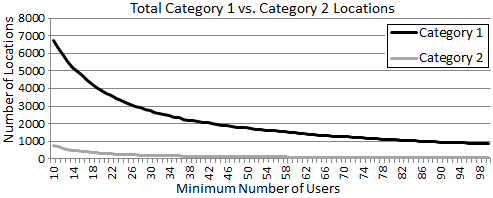
\includegraphics[width=5.4in]{Fig1}
\caption[Category 1 vs. Category 2 location frequency]{Category 1 are locations with a high accuracy where at least 75\% of users post messages with coordinates that are within 100 miles of coordinates geocoded from the self-reported location. Category 2 has low accuracy where less than 3.4\% of users match.}
\label{fig_ch2_1}
\end{figure}

\section{Classifier for Identifying Poor Geocoding}

Google's geocoder will attempt to geocode queries such as `my house' by matching to a business name. Such self-reported locations are common on Twitter due to the user being purposely ambiguous to preserve privacy. The classifier utilizes features, such as overlap between query and geocoder's associated address components, in order to make a prediction of whether Google's geocoder should be trusted.

\subsection{Features}

\begin{table}
\small
\renewcommand{\arraystretch}{1.2}
\caption{Google Geocoder Output}
\label{table_ch2_4}
\centering
\begin{tabular}{|c|c|}
\multicolumn{2}{c}{Additional Google Geocoder Output besides Coordinates}\\
\hline
\bfseries Output Type & \bfseries Description\\
\hline
address & Each component consists of the component type, short name, \\
components & and long name. Example types are country, ADM1 (state), \\
& ADM2 (county), locality (city), street number, route, \\
& neighborhood name, postal code, and others. \\
 \hline
formatted address&	Full address matched by Google, may not include all of \\
& the address components (for example county usually omitted). \\
 \hline
address & Describes what the address is associated with, example values: \\
type & point of interest, university, restaurant, and others. \\
\hline
\multicolumn{2}{c}{}\\
\multicolumn{2}{c}{Google Geocoder Output for query `New York, New York'}\\
\hline
\bfseries Output Type & \bfseries Output Value\\
\hline
coordinates & lat: 36.1023715, lng: -115.1745559\\
\hline
address & street\_number: 3790, route: South Las Vegas Boulevard\\
components & locality: Las Vegas, ADM2: Clark County, ADM1:\\
& Nevada, country: United States, postal\_code: 89109\\
\hline
formatted address& 3790 S Las Vegas Blvd, Las Vegas, NV 89109, USA\\
\hline
address type & casino, establishment, lodging, point\_of\_interest\\
\hline
\end{tabular}
\end{table}

\begin{table}
\small
\renewcommand{\arraystretch}{1.2}
\caption[Top 10 Most Frequent Address Type and Address Component]{Top 10 Most Frequent Address Type (Left) and Component (Right)}
\label{table_ch2_6}
\centering
\begin{tabular}{|c|c||c|c|}
\hline
\bfseries Address Type & \bfseries Ratio & \bfseries Address Component & \bfseries Ratio \\
\hline
political&0.6298&country&1\\
\hline
locality&0.566&administrative\_area\_level\_1&1\\
\hline
establishment&0.3101&locality&0.9639\\
\hline
point\_of\_interest&0.3068&administrative\_area\_level\_2&0.9481\\
\hline
store&0.0563&postal\_code&0.5652\\
\hline
food&0.0511&route&0.3348\\
\hline
neighborhood&0.04&street\_number&0.3027\\
\hline
restaurant&0.0395&administrative\_area\_level\_3&0.2005\\
\hline
university&0.0249&neighborhood&0.1827\\
\hline
route&0.0246&postal\_code\_suffix&0.1308\\
\hline
\end{tabular}
\end{table}

Table \ref{table_ch2_4} shows additional output, Google's geocoder produces, besides the latitude and longitude coordinates, and gives as an example, the output for query `New York, New York'. Notice that for the query, the street number in address components as well as the address types: (i) casino, (ii) establishment, (iii) lodging are indicative of an address that is a street level address (which could be used to assign a lower confidence for this prediction).

Across all of the locations in our dataset, there were a total of 73 unique address components and 116 unique address types. Table \ref{table_ch2_6} shows the top 10 address components and address types that account for the biggest ratio of all locations. The address types of store, food, restaurant should not represent a plausible location that most Twitter users will associate themselves with, but surprisingly over 5\% of locations in our dataset are some sort of a store (indicating potential errors). 

After looking at all address components, our expectation was that most Twitter users will report a location that is associated with: (i) political entity, (ii) zip, or (iii) university address type (as these are large enough to be reasonable locations to associate with). A location with one or more of these attributes is classified as a high-level location; otherwise, it is classified as low-level (street-level). 

\begin{figure*}[htp]
\centering
   \subfloat[Category 1]{\label{fig_ch2_2a}
      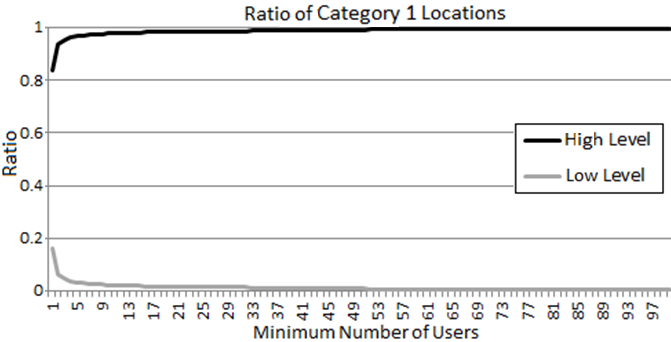
\includegraphics[width=.74\textwidth]{Fig2}}
\\
   %\hspace*{\fill}   % maximize separation between the subfigures
   \subfloat[Category 2]{\label{fig_ch2_2b}
      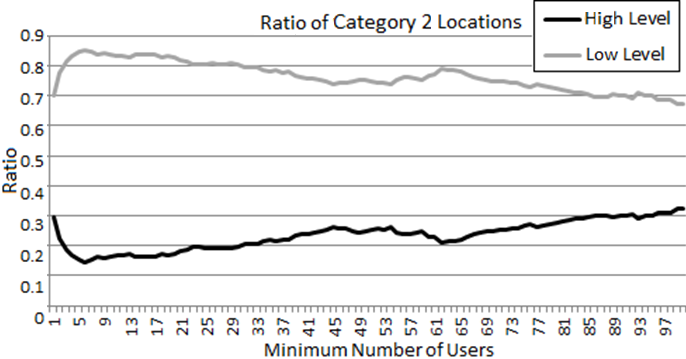
\includegraphics[width=.74\textwidth]{Fig3}}
   \caption[Category 1 vs. Category 2 ratio street-level]{\textbf{Top} -- Large ratio of Category 1 locations associated with a high-level address (as in city-level). \textbf{Bottom} -- Large ratio of Category 2 locations (impossible to geocode) are associated with low-level (as in street-level). The chart confirms that majority of properly geocoded locations are not at street-level.} \label{fig_ch2_2}
\end{figure*}

Fig. \ref{fig_ch2_2} (top) shows that the majority of category 1 locations get associated with a high-level location type. This is especially true as the minimum number of users that utilize location increases. For locations with number of users $\geq 100$, the high-level location type captures 99.6\% (843 out of 846) of category 1 locations. 

Conversely, Fig. \ref{fig_ch2_2} (bottom) shows inaccurately geocoded locations captured by category 2 are associated with low-level location type. The overall trend does not decrease, but the number of associated mistakes is small because the number of category 2 locations is small (only 43 locations used by at least 100 users). %$\geq 100$ per location the high-level location type captures 32.56\% (14 out of 43) of category 2 locations. 
Examples of locations that do get associated with a high-level location type: Midwest to Midwest WY, Nederland to Nederland CO, Nowhere to Nowhere OK, Moon to Moon PA, and others where a popular concept matches a city name. 

A number of additional features were proposed based on overlap between query and geocoder association. All of the features proposed are summarized below:

\begin{itemize}
\item F1: Political Entity = political address type without a street number address component. The political address type refers to recognized divisions of a physical territory; locality, neighborhood, colloquial area, sub-locality, and others.
\item F2: Zip = postal code address type
\item F3: University = university address type
\item F4: Text Overlap = returns percent character overlap between textual self-reported location and textual address associated by the geocoder.
\item F5: City/State exact = returns true if tokens from the query can be combined to match city and state address component exactly, false otherwise. 
\item F6: Populous City = for unique cities with a population over 50K, it is assumed that city name may be known to most human users such that the state need not be spelled out. Location matched to 2016 US census data using city and state that Google associates with the query string.
\end{itemize}

\subsection{Classifier}

Accurately geocoded locations (TRUE label) are those with $ACC@100$ $\geq$ 0.75 (category 1). Impossible to geocode locations (FALSE label) are those with $ACC@100$ $\leq$ 0.035 (category 2) (each self-reported location used by at least fifty users). The classifier utilizes the proposed features for predicting when Google's geocoder will perform poorly. 

For the classifier, we considered Naïve Bayes and Decision Tree (using gain ratio, information gain, and Chi-square interaction detector (CHAID)). Classifier trained using 5-fold-cross-validation utilizing the RapidMiner software package. Fig. \ref{fig_ch2_4} shows, the best performing classifier, Decision Tree using the CHAID criterion. 

\subsection{Performance}

Table \ref{table_ch2_7} compares the performance using three error measures proposed for locations that pass and fail classifier. Out of 131,925 self-reported locations in our dataset, 46,091 or 35\% were classified as low confidence (Google geocoder's output should not be trusted for these). Under 20\% of users with such locations are confirmed using message coordinates (illustrating that they do indeed have poor performance). In contrast, for those locations that pass the classifier, over 80\% of users are confirmed via message coordinates.   


\begin{figure}[!t]
\centering
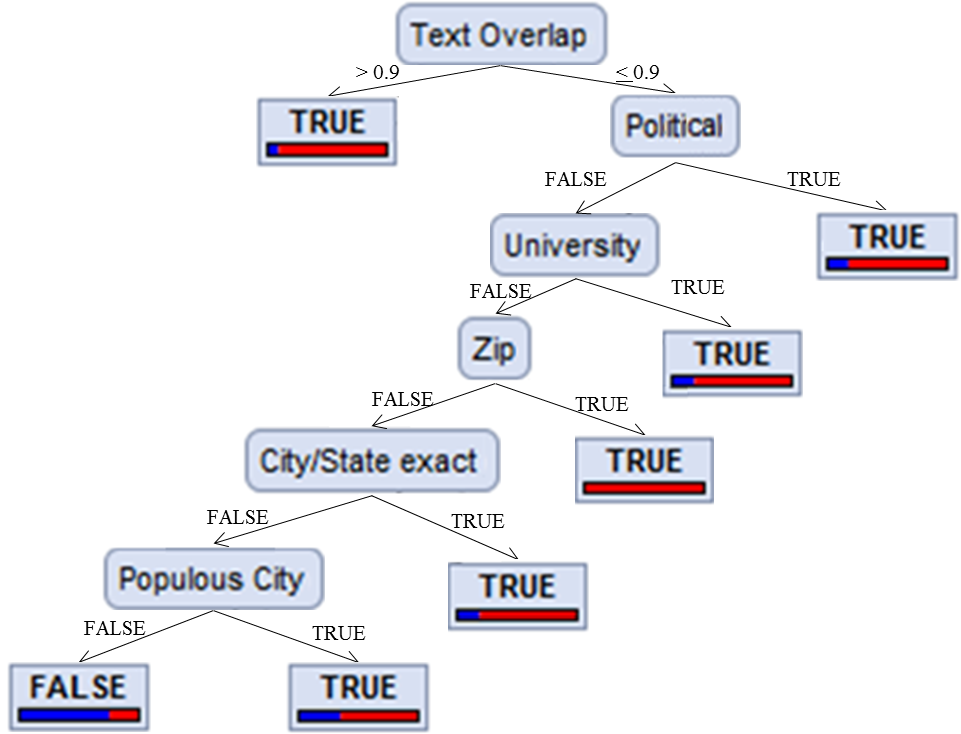
\includegraphics[width=3in]{Fig4}
\caption{Decision Tree Classifier for Identifying Geocoding Errors}
\label{fig_ch2_4}
\end{figure}

\begin{table}
\small
\renewcommand{\arraystretch}{1.2}
\caption{Geocoding Performance over Users}
\label{table_ch2_7}
\centering
\begin{tabular}{|c|c|c|c|}
\hline
\bfseries Location Set & \bfseries MeanED & \bfseries MedianED & \bfseries ACC@100\\
\hline
Fail Classifier&1705.12&879.45&0.1969\\
\hline
Pass Classifier&237.1&6.3&0.8027\\
\hline
\end{tabular}
\end{table}

The rules of the classifier illustrate that it is important to consider whether a location that is matched by the geocoder contains both the city and state as this is less ambiguous than a city name by itself. Google's geocoder is limited by the amount of API calls it can freely make daily and thus matching using a rule-based approach (using locations that contain a known city/state or city/country) is an option for a high precision/low recall solution.

\section{Conclusions}
The research has explored various types of geocoding errors and has established expected error rates for well and poorly geocoded locations in the context of Twitter. These measures were used to develop a classifier for whether the commercial off-the-shelf geocoder is performing as it should on Twitter data. In our dataset, close to 35\% of self-reported locations geocoded using Google resulted in a warning. Under 20\% of users with such locations were confirmed using message coordinates, illustrating that the Geocoder does exhibit a poor performance for these locations. In contrast, for those locations that pass the classifier, over 80\% of users are confirmed via message coordinates. In the next chapters, for those users whose location cannot be determined from textual self-reported location, other features will be described for inferring location.
\graphicspath{{Paper3Figures/}}
\chapter{Identifying Local Influencers and City-Level Communities}\label{chap3}

\setlength{\abovedisplayskip}{-10pt} \setlength{\abovedisplayshortskip}{-10pt}

\section{Background}
User's popularity on Twitter can be measured by how well the user is recognized by others, such as through others' mentions and follows. Understanding the location of popular users is needed for content recommendation and other use cases. For example, an advertising agency, that is performing a city-wide promotion, will be interested in users that serve important roles within that city such as the city's mayor. Generating crime statistics across cities could require focusing on local fire, police, and other emergency related influencers. Tracking sports could require tracking local football, basketball, baseball, and others relevant to the city of interest. 

The standard approach first geocodes a large number of users using each user's self-reported location. Second, the users whose locations map to within $x$ miles of the city of interest are used to establish the city-level community. As has already been noted in Chapter 2, the biggest obstacle to this approach is the lack of a good geocoding solution. 

In contrast, our approach does not require geocoding and instead leverages the power of Google search along with the follow structure on Twitter. We found that querying for (city, state, plus keyword `Twitter') is likely to return Twitter influencers that are specific to the city (geo-influencers). The geo-influencer's followers form the basis of a city-community. The benefit is that many of the followers may not contain a geocodable self-reported location, but make it in as part of our approach (this is because following a geo-influencer serves as a strong indicator of the follower's location). Following a local police department and local traffic updates serve as a strong indicator of the user's location even if the user does not list a geocodable self-reported location field. 
 
The Term Frequency-Inverse Document Frequency (TF-IDF), where the Term Frequency measures the number of follows by the community, is used to produce a ranked list of most popular geo-influencers. In this way, by fusing the power of Google for finding initial geo-influencers and the crowd-sourcing power of the underlying Twitter community, we can associate hundreds of additional city-level geo-influencers and use these to further refine the city-community. A ranking of national-level influencers are those with followers across multiple city-level communities.

\section{Related Research}

There is a great amount of research related to Twitter user's activity, popularity, and influence [\ref{appendix:2.1}]. Activity measures actions that a user takes (such as tweets, retweets, mentions, and replies); influence measures whether user's actions are capable of affecting other users' actions in the network; and popularity measures how well the user is recognized such as through others users' mentions and follows. In this research, we are focusing on popularity through other user's follows. This work is related to Location-Aware Influence Maximization (LAIM) [\ref{appendix:2.2}, \ref{appendix:2.3}], where the goal is to identify top k users to maximize the expected number of influenced users in a specific geographical area. 

%In popularity ranking an essential step is to establish a community of users over which it is computed. 
Multiple features can be used to establish a community of users with some features in common [\ref{appendix:2.4}]. For example,  (i) structure-based features where two users both follow the same influencer [\ref{appendix:2.5}-\ref{appendix:2.8}], (ii) activity-based features such as how frequently and during what times the user is active [\ref{appendix:2.9}-\ref{appendix:2.11}], (iii) content-based features such as the type of users, topics, URLs being mentioned [\ref{appendix:2.12}-\ref{appendix:2.14}], and (iv) communication-based features such as retweet, reply, and mention [\ref{appendix:2.15}, \ref{appendix:2.16}]. 

The second step is to associate users with a geographical area (usually at the city-level). The user's location may be geocoded from the self-reported profile location or aggregated from coordinates in the user's tweets [\ref{appendix:1.1}]. For a user without location information, the median of user's friends' location can be used [\ref{appendix:1.11}, \ref{appendix:2.19}].% These approaches suffer due to a high level of noise associated with geocoding locations. For example, tweets with precise GPS coordinate point are limited to 1\% of the overall Twitter stream and may not refer to a user's home location [\ref{appendix:1.12}]. The self-reported profile location may be available for over a third of users, but needs to be geocoded and is prone to ambiguous locations like `Planet Earth' [\ref{appendix:1.2}].

Finally, once the communities and the underlying geographical locations are known, the ranking of the users for each geographical area can be done using traditional graph metrics such as degree centrality [\ref{appendix:2.22}], custom measures that for example punish spammers [\ref{appendix:2.23}], and variations on PageRank [\ref{appendix:2.24}-\ref{appendix:2.26}]. 

A recent paper, that is most directly related to our research, explores the problem of identifying relevant geo-influencers across three US cities: Boston MA, Bristol CT and Seattle WA [\ref{appendix:2.26}]. Their network was built using social activity based interactions retweet, reply, and mention present in over five billion tweets. They relied on self-reported profile location information for extracting a ranked list of influential users whose location is within 100km of the city of interest. The ranking was performed via several modified PageRank based algorithms. They showed that self-reported locations were needed for filtering out global users that are not from the area such as @YouTube. However, it was also shown that limiting users within $x$ miles of the location of interest would filter out other important users, such as @Patriots, that had a strong local connection spanning beyond 100 km.

We propose a novel way of performing a targeted collection that results in a community of users for each city location. For each city, the communities stem from an initial pool of influential users identified via automatic Google searches. Our approach does not rely on any location information. In this way, each community may contain passive readers that do not tweet and users with no location information. Most importantly our city communities are made up of followers of geo-influencers that are known to be associated with the city of interest. A modified TF-IDF measure results in ranked lists that perform well against hand-labeled data including data from [\ref{appendix:2.26}], but the overall collection requirements are magnitudes smaller.

\section{Approach}
Given a city of interest and a list of other cities from which to distinguish, our approach will follow the process outlined in Fig. 3.1. The figure shows four main steps: (1) Google search to discover known geo-influencers for each city, (2) ordinary followers of geo-influencers from step 1 are used to establish a city community, (3) collect friends of the city community from step 2, and (4) a modified TF-IDF measure is used to identify geo-influencers from step 3. In our work, we define `an ordinary follower' as one who has between 20 and 100 friends, less than 500 followers, not verified by Twitter, without a URL, and that does not generate over five tweets per day since created. An influencer is simply a user with at least 500 followers.

Steps 1-3 shown on the left side of Fig. 3.1 are repeated for each city after which step 4, illustrated on the right, is applied. Each component of the process from Fig. 3.1 is described in more detail in the subsections below.

\begin{figure}[!t]
\centering
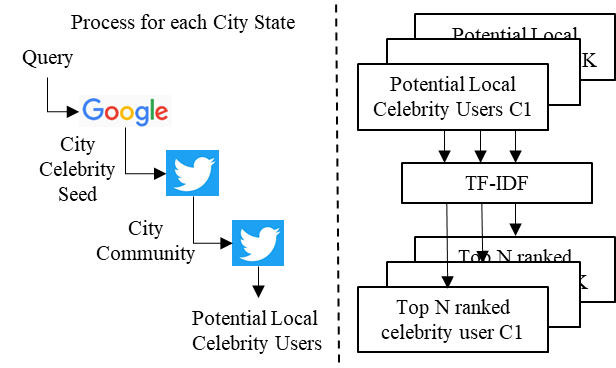
\includegraphics[width=4in]{Fig1}
\caption{Top N geo-influencers extracted from K Cities}
\label{fig_ch3_1}
\end{figure}

\noindent\textbf{Step 1: Google Queries for getting the Initial Geo-Influencers}-- Given a query that consists of (city, state, `Twitter') (and an optional keyword such as `Sports') Google returns a list of URLs. In the first 100 Google hits, our interest is in the following URL structure: `https://twitter.com/' + screenname + `?lang=en'. We record the screenname and the associated URL hit number. In this manner, Google search associates influencers with a city. In our work, the top ten influencers are used. By utilizing optional keywords, such as `News' or `Sports', we can focus on the geo-influencers by topic. For example, the query `Syracuse, NY Twitter News' results in the top three news-related influencers: @SyracuseUNews, @syracusedotcom, and @NewsChannel9. 

\noindent\textbf{Step 2: Initial Geo-Influencers to City Community}-- Twitter API is used to collect followers of initial geo-influencers; thus forming the basis of the city community. According to a 2016 Twitter SEC filing, approximately 8.5\% of all Twitter users are bots [\ref{appendix:2.27}]. Bots have many connections and post many messages. Thus, to avoid/minimize bots we focus on ordinary followers (one of the criteria is not posting over five messages a day). To focus on the users that are interested in a single city, we also ensure that city-communities are disjoint, i.e., no user belongs to two or more communities.  

\noindent\textbf{Step 3: City Community to Additional Geo-Influencers}-- Twitter API is used to collect friends of users that make up the city community; users with over 500 followers form a pool of additional `potential' geo-influencers; potential because influencers which are popular across multiple cities may be included (TF-IDF measure helps filter these out).

\noindent\textbf{Step 4: Ranking via TF-IDF}-- As mentioned earlier, traditional approaches find the influencers using network based methods, such as the degree centrality or PageRank. In our research, we apply TF-IDF, which is intended to reflect how important a word is to a document in a corpus. To apply TF-IDF measure it was critical to have well defined city communities (those consisting of users that are from the city). For each city, a document is made up of all potential geo-influencers that the city community has made a connection to. The process shown on the left in Fig. 3.1 builds such a document for each city.

Let C represent the set of all cities, community($c_v$) return the set of ordinary followers that make up the community for city $c_v$, and friends($o_w$) return the set of influencers that the user $o_w$ follows:

\begin{itemize}
\item C = \{$c_1$, $c_2$, ..., $c_k$\}
\item community($c_v$) = \{$o_1$, $o_2$, ..., $o_m$\}
\item friends($o_w$) = \{$u_1$, $u_2$, ..., $u_n$\}
\end{itemize}

Term frequency for user $u_x$ and community $c_v$ corresponds to total friend connections to user $u_x$ within community divided by total friend connections: 

\begin{equation}
TF(u_x, c_v) = \frac{\sum_{o \epsilon community(c_v)} |u_x \epsilon friends(o)|}{\sum_{o \epsilon community(c_v)} |friends(o)|}
\end{equation}

As an example, given community($c_1$) = \{$o_1$, $o_2$, $o_3$\} where friends($o_1$) = \{$u_1$, $u_2$\}, friends($o_2$) =\{$u_2$, $u_3$\}, and friends($o_3$) = \{$u_1$, $u_2$, $u_3$\}: TF($u_1$, $c_1$) =(1+0+1)/(2+2+3) = 2/7, similarly TF($u_2$, $c_1$) = 3/7 and TF($u_3$, $c_1$) = 2/7.

Inverse document frequency is given by the total number of cities divided by the number of cities user $u_x$ has a connection to (cities where that user is mentioned more than once):

\begin{IEEEeqnarray}{rCl}
IDF(u_x) & = & \log \biggl(\frac{|C|}{\sum_{c_v \epsilon C}|\{TF(u_x, c_v) > 0\}|} \biggr)
\end{IEEEeqnarray}

As an example, given another community($c_2$) = \{$o_4$\} where friends($o_4$) = \{$u_1$, $u_4$\}: IDF($u_1$) = log(2/(1+1)) = 0 and IDF($u_4$) = log(2/(0+1)) = log(2).

Combining formula 1 and 2 gives a formula for ranking a potential influencer $u_x$ for community $c_v$:

\begin{equation}
TF-IDF(u_x, c_v) = TF(u_x, c_v)*IDF(u_x)
\end{equation}

\section{Data}
Using the data from the 2016 Census Bureau we focused on known cities in the USA. We built a set of cities by initially starting with the most populous city and incrementally adding other most populous cities as long as they were at least 30 miles apart from cities already in the set. This ensured that the selected cities were geographically spread apart. The set so obtained contained 264 (city, state) pairs.

The process in Fig. 3.1 was used to generate three datasets based on three different keywords that made up the Google query: (i) Twitter, (ii) Twitter News, and (iii) Twitter Sports. Out of 264 cities, only 64 cities contained at least ten geo-influencers for each search type. Followers of geo-influencers were used to establish each city community. The followers that simultaneously follow many geo-influencers were prioritized. It was required that each city community have at least 100 and at most 1000 users. Fig. 3.2 shows the collection process for the network associated with each city and the corresponding maximum network size.

\begin{figure}[!t]
\centering
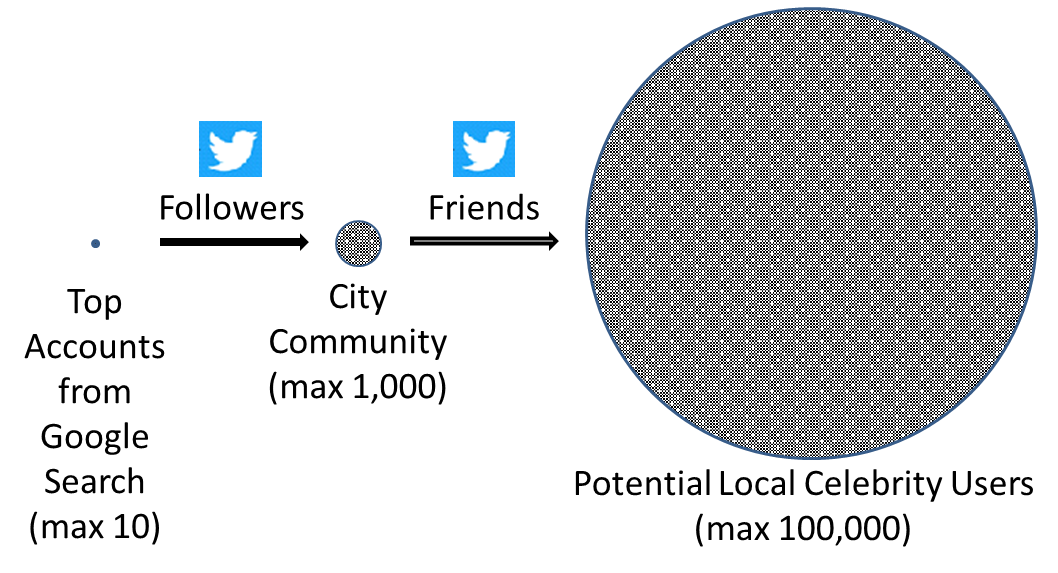
\includegraphics[width=4in]{Fig2}
\caption[Collection from seed, to city-community, to set of influencers]{Collection process from initial influencers to city-level community to a new set of influencers (drawn to scale)}
\label{fig_ch3_2}
\end{figure}

In addition to the three datasets described above, we obtained the fourth dataset where the city community is made up of users whose self-reported locations were verified via geocoder (using Google Maps API\footnote{https://developers.google.com/maps/documentation/geocoding}) to within 10 miles of city's (latitude, longitude). For this dataset, ordinary followers were selected from the followers of major news outlets: ABC, Politico, PBS, WSJ, Fox News, Reuters, CNN, and MSNBC. For each city community, we collected at least 100 users but at most 1/500 of the city's population. Out of the 64 cities covered by the other three datasets, only 19 cities provided a large enough sample size. These 19 city communities across the four datasets were: Charlotte NC, Washington DC, Wichita KS, Tucson AZ, Denver CO, Madison WI, San Diego CA, Syracuse NY, Lansing MI, Toledo OH, Boston MA, Columbia MO, Chicago IL, Springfield MO, Rochester NY, Lubbock TX, Atlanta GA, Topeka KS, and Albany NY.

Comparing results from the first three datasets showed the effect of differing queries, i.e., how the resulting communities differ in geo-influencer ranking. The fourth dataset allows us to compare how the city community generated via geo information differs from community based on follow connections to Google identified influencers. Table 3.1 summarizes the four datasets collected across these 19 cities. Table 3.1 shows the number of users, average, and standard deviation per community. From the table, we see that Dataset 4 has a high standard deviation, i.e., due to bigger samples for bigger cities. Dataset 3, related to `Twitter Sports', has a smaller community than the more general topics: `Twitter' and `Twitter News'.

\begin{table}
\small
\renewcommand{\arraystretch}{1.2}
\caption[Dataset Statistics across 19 Cities that occur within each dataset.]{Dataset Statistics across 19 Cities that occur within each dataset. The total number of users across the 19 city-communities is shown as well as the average number of users per city-community and the associated standard deviation.}
\label{table_ch3_1}
\centering
\begin{tabular}{|c|c|c|c|c|}
\hline
\bfseries Set & \bfseries Seed Type & \bfseries Avg & \bfseries Stnd & \bfseries Total \\
\hline
D1&Google using Twitter&692.21&203.52&13152\\
\hline
D2&Google using Twitter News&728.95&198.35&13850\\
\hline
D3&Google using Twitter Sports&516.32&324.30&9810\\
\hline
D4&Major National News&726.79&944.03&13809\\
\hline
\end{tabular}
\end{table}

\section{Evaluation}

\subsection{Impact of Keyword in Google query on Final Rank}

\begin{figure}[!t]
\centering
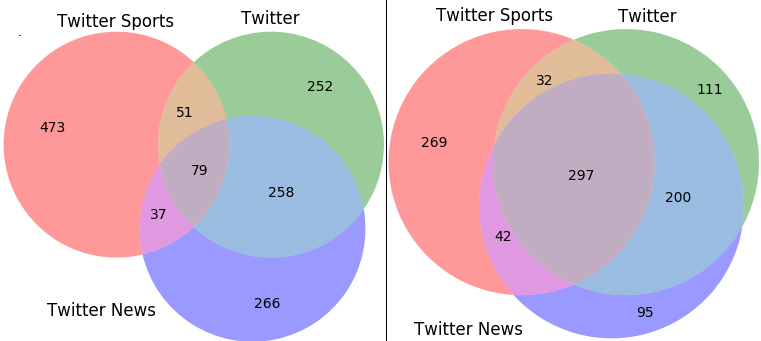
\includegraphics[width=5in]{Fig3}
\caption[Seed vs. Top Ranked Influencer Overlap Venn Diagram across 64 cities]{Seed Twitter User Overlap (left) vs. Top Ranked User Overlap (right) across 64 cities for the three search types). While the initial queries produce an initial set of influencers (seed) that differ (shown on the left), the resulting influencers that are extracted from city-level communities formed from seed have quite a bit of overlap (shown on the right). This illustrates that the method is robust in that different influencers can be used as a seed to get to the same end result (as long as the initial influencers are indeed local to the city of interest).}
\label{fig_ch3_3}
\end{figure}

We analyzed the first three datasets. The ground truth, in this case, are the geo-influencers using Google search. Each dataset contained 640 geo-influencers across 64 cities (1920 for all three datasets). Venn diagram in Fig. 3.3 (left) shows 79 out of 1920 or 4.1\% of geo-influencers associated by Google overlap across three search types with more overlap between Twitter and Twitter News. Ranked list via TF-IDF, Venn diagram of Fig. 3.3 (right) shows a more significant overlap, 297 out of 1914 or 15.5\% of users. The figure shows that on average more than half of ranked geo-influencers overlap (with Twitter and Twitter News being most aligned). This illustrates that different initial geo-influencers can lead to similar final rankings.

\subsection{Performance against Google Ranked Geo-Influencers}

Google is driven by those webpages that a user is most likely to click on while the number of followers drives Twitter's popularity. In the majority of cases we have found that there is an overlap between Google associated users and top-ranked users via TF-IDF, especially as $n$ increases. We calculated the ratio of overlap between the two as:

\begin{equation}
Overlap(X(c_v), Y(c_v,d,n)) = \frac{|X(c_v) \cap Y(c_v,d,n)|}{|X(c_v)|}
\end{equation}

Where X($c_v$) refers to a set of known geo-influencers that are associated with city $c_v$ from Google and Y($c_v$, $d$, $n$) refers to top $n$ ranked influencers stemming from the TF-IDF measure for city $c_v$ and dataset $d$. 

The top ten geo-influencers across three Google search types are combined providing a larger set to compare against (24.58 geo-influencers on average). Fig. 3.4 shows, for each dataset, the average percent of Google geo-influencers confirmed by each query type as the ranked list grows in size. The metric is averaged across 19 cities that are present in each of the four datasets. Despite each dataset representing slightly differing communities, due to having been formed using different seeds, we see that they all confirm a similarly large portion of geo-influencers that were deemed relevant by Google with generic Twitter search type working the best.

\begin{figure}[!t]
\centering
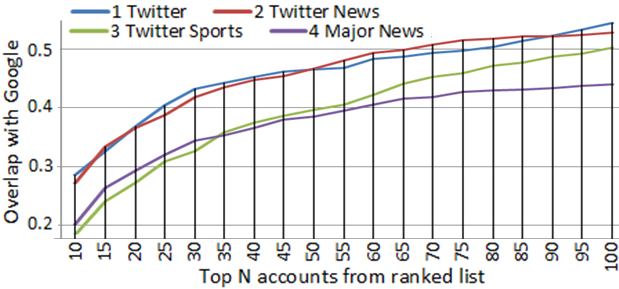
\includegraphics[width=4in]{Fig4}
\caption[Percent of Google geo-influencers confirmed by each query type]{Percent of Google geo-influencers confirmed by each query type as the ranked list grows in size. Followers of major news that were verified via geocoder follow similar influencers as returned from Google.}
\label{fig_ch3_4}
\end{figure}

In a similar fashion, Table 3.2 shows the top 30 geo-influencers using TF-IDF vs. top ten geo-influencers for each Google search type. The last row is a combination of the top ten Google geo-influencers across datasets D1-D3, also used in Fig. 3.4. Ratios in bold highlight the best aligning datasets. It could be argued that each dataset simply confirms the same initial seed that was used to establish the dataset. D4 was established, to illustrate that communities established without leveraging Google would also confirm them. Communities from D4 were established from self-reported locations of followers following major news influencers and hence did not utilize Google in any way. Despite this D4 had a high overlap for Twitter News search type (0.61, this overlap helps confirm that the proposed approach can work in a similar fashion as the one that relies on geocoding).

\begin{table}
\small
\renewcommand{\arraystretch}{1.2}
\caption{Overlap for Geo-Influencers from Google vs. Dataset}
\label{table_ch3_2}
\centering
\begin{tabular}{|c|c|c|c|c|}
\hline
\bfseries Search Type (X) & \bfseries D1 & \bfseries D2 News & \bfseries D3 Sports & \bfseries D4 News \\
\hline
Twitter&\bfseries 0.69&0.62&0.37&0.55\\
\hline
Twitter News&0.71&\bfseries 0.74&0.47&0.61\\
\hline
Twitter Sports&0.12&0.12&\bfseries 0.28&0.08\\
\hline
all&\bfseries 0.43&0.42&0.33&0.34\\
\hline
\end{tabular}
\end{table}

Next, we focus on Google geo-influencers that do not make it into ranked lists even for very large n. For instance, for n=1000 there were 67 such geo-influencers. We checked each of the 67 geo-influencers by hand. 37 out of 67 geo-influencers were found accurate, but all had fewer than 500 followers to be considered by our method. These referred to local high schools, local businesses, small local sports teams related to tennis, volleyball, and others. To incorporate these geo-influencers, we would need to change our threshold for influencer from 500 to 100 followers.

Next, examples of Google geo-influencers that were found inaccurate. @CityofToledo has never tweeted, with 105 followers, being in the fourth search result for the query `Toledo OH Twitter' (this is probably due to close overlap in keywords with @city\_of\_toledo the first search result and official city account). Some influencers have a national follower base, but are associated with a single city such as @RiddellSports associated with `Chicago, IL Twitter Sports'. Google search results fluctuate over time with about two-thirds of the 67 accounts no longer recommended after the search was repeated about a month later. Hence verification is still recommended for optimal results when establishing initial geo-influencers from which each city community is to be established.

\subsection{Communities via Location vs. Google Seed}

Dataset D4 was established using followers of major national news outlets whose self-reported location could be associated with the city of interest. The issue with self-reported locations is that less than a quarter of all users had locations that could be geocoded. Also, we found geocoding errors for example `Salem' was associated with `Salem, MA', but often the location referred to Salem which is in India. As a result, we focused on high confidence locations that specify both city and state, but such locations were challenging to find for smaller cities despite collecting on millions of users.
 
The benefit of datasets D1-D3 is that they were assembled much quicker than D4 and they covered many more cities with more users per city. For users in D1-D3, over 64 city communities, the percent of users with the non-empty self-reported location was only 28.2\%. For those users that did specify their location, on average 41.6\% contained the city name associated by our method, thus illustrating that these communities are well structured.

\subsection{City Level Evaluation}
\begin{table}
\small
\renewcommand{\arraystretch}{1.2}
\caption{Top 30 Geo-Influencers extracted from each Dataset}
\label{table_ch3_3}
\centering
\tabcolsep=0.09cm
\begin{tabular}{|c|c|c|c|}
\hline
\bfseries D1&\bfseries D2 News&\bfseries D3 Sports&\bfseries D4 News\\
\hline
\bfseries marty\_walsh&boston25&\bfseries cityofboston&visitbostoncity\\
\hline
\bfseries cityofboston&\bfseries 7news&hiddenboston&\bfseries cityofboston\\
\hline
\bfseries bostondotcom&\bfseries wcvb&\bfseries wcvb&\bfseries bostondotcom\\
\hline
bostontweet&\bfseries bostondotcom&\bfseries marty\_walsh&\bfseries marty\_walsh\\
\hline
mbta&\bfseries bostonpolice&eatboston&bostontweet\\
\hline
onlyinbos&onlyinbos&\bfseries bostondotcom&mbta\\
\hline
\bfseries 7news&massstatepolice&bostontweet&bostonmagazine\\
\hline
\bfseries bostonpolice&bostonglobe&mbta&\bfseries bostonfire\\
\hline
bostonmagazine&mbta&bostonmagazine&\bfseries 7news\\
\hline
massgovernor&\bfseries cityofboston&boston25&\bfseries bostonpolice\\
\hline
\bfseries wcvb&\bfseries marty\_walsh&massstatepolice&mayortommenino\\
\hline
hiddenboston&massgovernor&massdot&massdot\\
\hline
boston25&bostonmagazine&\bfseries 7news&eatboston\\
\hline
bostonglobe&bostontweet&\bfseries bostonfire&bplboston\\
\hline
massstatepolice&\bfseries wbz&massgov&\bfseries wcvb\\
\hline
bostinno&985thesportshub&theimproper&bostonglobe\\
\hline
bostonpwd&\bfseries nhlbruins&\bfseries bostonpolice&massgovernor\\
\hline
\bfseries nhlbruins&scottzolak&bosbizjournal&massgov\\
\hline
stoolpresidente&jerry\_remy&\bfseries wbz&boston25\\
\hline
edelman11&stoolpresidente&mbta\_alerts&massstatepolice\\
\hline
\bfseries wbz&wilfork75&massema&bostonparksdept\\
\hline
theimproper&hiddenboston&mbtatransitpd&bostinno\\
\hline
\bfseries bostonfire&justamasshole&eaterboston&theimproper\\
\hline
\bfseries redsox&lowellsunnews&massgovernor&hiddenboston\\
\hline
\bfseries celtics&\bfseries celtics&harveywcvb&\bfseries wbz\\
\hline
bos311&edelman11&universalhub&visitma\\
\hline
universalhub&bostinno&mayortommenino&universalhub\\
\hline
bostonbtd&theimproper&bostinno&onlyinbos\\
\hline
jerry\_remy&toucherandrich&985thesportshub&bostoncalendar\\
\hline
\bfseries bostonherald&nesn&fredtoucher&bostonschools\\
\hline
\end{tabular}
\end{table}

Evaluation in [\ref{appendix:2.26}] listed ground truth for Boston MA via these 20 geo-influencers: (i) News = wcvb, bostondotcom, cbsboston, 7news, bostonherald, (ii) Sports = redsox, celtics, nhlbruins, thebostonpride, bostoncannons, (iii) Gov = marty\_walsh, cityofboston, bostonpolice, bostonfire, masddot, and (iv) University = bu\_tweets, harvard, mit, berkleecollege, northeastern (influencer cbsboston renamed to wbz). The top five for the best performing ranked list from [\ref{appendix:2.26}] contained: Patriots, BostonGlobe, OnlyInBOS, RedSox, and NHLBruins (so in their approach the last two matched the ground truth). For our approach, table 3.3 shows the top 30 geo-influencers (those in bold match the ground truth).

Our approach carries as many as four matches in the top five and as many as twelve matches in the top thirty geo-influencers. This compares favorably to the results reported in [\ref{appendix:2.26}]: two matches in the top five and eleven matches in the top thirty influencers. None of our ranked lists incorporate high-level influencers such as @YouTube. Furthermore, our approach allows targeted city collection which results in an overall network being orders of magnitude smaller. As was shown in Fig. 3.2 there are at most 100,000 users collected per city. 

A number of geo-influencers overlap across the four datasets. This again reinforces that similar results can be achieved via differing city communities as long as those communities are local to the city. What differentiates communities is that the ranking will be slightly tilted towards the query. For example, Table 3.4 shows geo-influencers, and the position in the ranked list of 1000, that contain the keyword `Celtics' (a popular basketball team associated with Boston). As expected, D3 produces the most sports related influencers (because query also contained `sports').

\begin{table}
\small
\renewcommand{\arraystretch}{1.2}
\caption{From each Dataset Top Geo-Influencers containing keyword Celtics}
\label{table_ch4_4}
\centering
\tabcolsep=0.13cm
\begin{tabular}{|c|c|c|c|}
\hline
\bfseries D1&\bfseries D2 News&\bfseries D3 Sports&\bfseries D4 News\\
\hline
celtics: 25&celtics: 25&bdcceltics: 149&celticsblog: 304\\
\hline
celticslife: 525&celticslife: 115&nbcsceltics: 199&nbcsceltics: 386\\
\hline
&&celtics: 226&celticslife: 424\\
\hline
&&r\_bostonceltics: 261&bdcceltics: 483\\
\hline
&&celticsviews: 293&celtics: 975\\
\hline
&&celticsfanclub: 596&\\
\hline
\end{tabular}
\end{table}

\section{Geo-Influencer Collection Runtime}

Typically it is assumed that the social graph has already been collected and then different algorithms use its structure and various features in an attempt to identify the most important nodes. The algorithms are evaluated based on accuracy and runtime. We noticed that the algorithm runtime is negligible compared to the data collection time i.e. it is not uncommon for a researcher to have spent a year collecting the dataset, a dataset that cannot be fully shared with others (only unique ids can be shared and crawling on ids can take about as long as starting a new collection from scratch), and the dataset may not work all that well for a scenario that targets a certain demographic.

Up to 1\% of all Twitter message traffic can be collected using the unfiltered stream of tweets (from our experiments around 4 million tweets a day). This may seem like a lot of data, but for a specific use-case such as the 2014 annexation of Crimea by Russia, there might not be that many messages from the area of interest. The method proposed in this chapter is useful for identifying influencers and corresponding user communities from a particular geographic area. As an illustration, we show the expected collection times for three methods:
\begin{itemize}
\item  M1: using the union of followers from multiple geo-influencers
\item M2: using followers of a well-known influencer (national or global like)
\item M3: using message traffic
\end{itemize}

For influencers, the self-reported locations of the followers are analyzed. For message traffic, the self-reported locations of the users that generated the message are analyzed. For this illustration, we are interested in forming communities for cities: Syracuse and Buffalo of USA. The users whose self-reported location matches one of the cities are recorded. Each self-report location is turned to lowercase and it is checked whether the city name is present within it.

The geo-influencers associated with a city are found via automated Google search. All of the Twitter influencers identified in the top 100 URLs by Google are utilized. %Here are the geo-influencers associated with:

\iffalse
\begin{itemize}
\item Buffalo (28 total): DAErieCountyNY, NWSBUFFALO, BfloBizFirst, SPECNewsBuffalo, WBFO, BPDAlerts, RedandBlack716, BFLO\_CC, Buffalo\_Schools, SURJBuffalo, markpoloncarz, USACE\_Buffalo, BuffaloSewer, BuffaloBills, MobBuffalo, BuffaloSabres, wnymedia, IIBuff, news4buffalo, BuffaloNiagara, ECDOH, WGRZ, TheBuffaloNews, MayorByronBrown, buffalo\_ny, BuffaloEats, FBNY\_WNY, WKBW
\item Syracuse (28 total): VisitSyracuse, SPECNewsCNY, Cusememes, LO\_Syracuse, SyracuseAirport, dailyorange, CNYCentral, syrbasketball, SyracusePolice, NYSFair, CuseWBB, chrsbakr, AndrewDonovan, SyracuseOn247, Cuse\_Tennis, SyracuseU, Stephen\_Bailey1, Cuse\_MBB, NewsChannel9, BenWalsh44, OnondagaCounty, Cuse, CuseFootball, AdrienneSmithTV, SyracuseUNews, syracusedotcom, syracuseITC, Syracuse1848
\end{itemize}
\fi

All of the followers for these geo-influencers were collected for each city; for Buffalo\footnote{Followers collected over Buffalo geo-influencers (28 total): DAErieCountyNY, NWSBUFFALO, BfloBizFirst, SPECNewsBuffalo, WBFO, BPDAlerts, RedandBlack716, BFLO\_CC, Buffalo\_Schools, SURJBuffalo, markpoloncarz, USACE\_Buffalo, BuffaloSewer, BuffaloBills, MobBuffalo, BuffaloSabres, wnymedia, IIBuff, news4buffalo, BuffaloNiagara, ECDOH, WGRZ, TheBuffaloNews, MayorByronBrown, buffalo\_ny, BuffaloEats, FBNY\_WNY, WKBW}, a total of 2767322 were processed vs. 1165345 for Syracuse\footnote{Followers collected over Syracuse geo-influencers (28 total): VisitSyracuse, SPECNewsCNY, Cusememes, LO\_Syracuse, SyracuseAirport, dailyorange, CNYCentral, syrbasketball, SyracusePolice, NYSFair, CuseWBB, chrsbakr, AndrewDonovan, SyracuseOn247, Cuse\_Tennis, SyracuseU, Stephen\_Bailey1, Cuse\_MBB, NewsChannel9, BenWalsh44, OnondagaCounty, Cuse, CuseFootball, AdrienneSmithTV, SyracuseUNews, syracusedotcom, syracuseITC, Syracuse1848} (some followers repeat across geo-influencers, number of unique followers were 1774172 vs. 566815, respectively). The collection time was 29.3 hours for Buffalo and 13.16 hours for Syracuse. Fig. \ref{fig_collectionRun} shows the number of unique followers that contain the city name in their self-reported location per 25000 followers for the two communities. The number of new followers with Syracuse in their self-reported location plateaus at around 20K. While the followers that contain Buffalo in their self-reported location continue to rise to 55K.

\begin{figure}[!t]
\centering
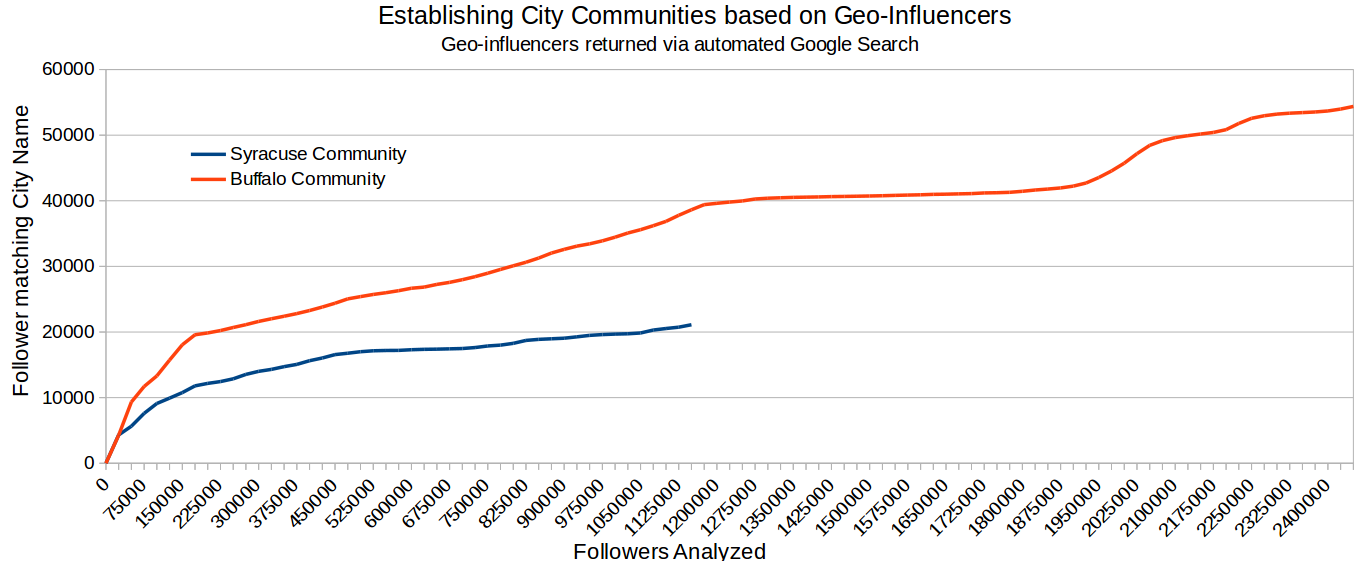
\includegraphics[width=5.6in]{Paper3Figures/FigCollectionRuntime.png}
\caption[Geo-Influencer Collection Runtime]{There is a large ratio of followers extracted with self-reported location matching the city of interest. Theoretically to process 25K in followers should take approximately 10 minutes. In this way in a relatively short time, in under 24 hours, a community of users that is representative of the city can be extracted. There is higher confidence in these users because they are known to follow a geo-influencer associated with the city as well as having the city in their self-reported location.}
\label{fig_collectionRun}
\end{figure}

Using influencer's followers it takes around 110 seconds to process 5000 followers\footnote{https://developer.twitter.com/en/docs/twitter-api/v1/rate-limits:\\GET followers/ids returns 5000 follower ids per minute, GET users/lookup can be used to process 900*100 ids per 15-minute interval or 100 followers per second. 60 seconds to collect 5000 followers ids plus 50 seconds to process ids gives 110 seconds.}. So theoretically, 3.92 million followers can be collected and processed daily. There are other factors impacting collection such as how quickly one can perform preprocessing and writes to a database which is why our collection times are a little different.

For method M2, using global/national like influencer, @NPR is used with 7.054M followers collected. This influencer was chosen because it is popular in the USA (a more global influencer like @CNN will perform worse as it will capture a smaller percentage of users for the cities in the USA). For message traffic a total of 10 million messages were collected (around 4 million messages daily). Table 3.5 shows how many users were extracted using each method divided by the total amount of time needed to perform the collection (time in hours). There is a much higher ratio of users for the city of interest from a collection that is focused on geo-influencers using method M1.

\begin{table}
\small
\renewcommand{\arraystretch}{1.2}
\caption{Average Number of Users (per hour) Matching City of Interest}
\label{table_abbr}
\centering
\begin{tabular}{|c|c|c|}
\hline
\bfseries users using method/collection time & \bfseries Syracuse & \bfseries Buffalo\\
\hline
method M1 based on geo-influencers & 21240/13.16=1614 & 56774/29.3=1938\\
\hline
method M2 based on global influencer & 1872/64.3=29 & 3994/64.3=62\\
\hline
method M3 based on message traffic & 283/57.36=5	 & 1048/57.36=18\\
\hline
\end{tabular}
\end{table}

Method M1 results in 21240 users for Syracuse and 56774 users for Buffalo. In comparison using message traffic to generate the same communities would require 21240/5/24=177 days and 56774/18/24=131 days respectively. For Syracuse, method M1 is 1614/5 = 322x and 1614/29 = 56x faster than method M2 and M3. For Buffalo, method M1 is 1938/18 = 107x and 1938/62 = 31x faster than method M2 and M3.

In a separate large collection of users based on followers of verified influencers (tracked by Twitter’s @verified) we collected 373 million profiles. This collection took over a year to complete. Across 373 million users, 42448 and 92276 contained Syracuse and Buffalo in their self-reported locations, respectively. This shows that the proposed M1 method can quickly identify roughly half of all Twitter users. The additional benefit in method M1 is that there is higher confidence in these users because they are known to follow a geo-influencer associated with the city as well as having the city in their self-reported location. 

Having identified the users that are representative of the demographic area, up to 3200 messages per user can be collected in a relatively quick amount of time\footnote{GET statuses/user\_timeline allows 900 requests per minute with each request providing up to 3200 Tweets (there is an additional limit to at most 100,000 requests per 24 hours)}. This will provide a larger set of relevant data than using the alternative methods we discussed. For example for Syracuse the 21240 users can be used to collect 15,206,890 messages and for Buffalo the 56774 users can be used to collect 54,913,648 messages. This is much more messages than can be collected in a day using the method M3 and these messages will be relevant to the geographic area of interest. The message creation times can be used to filter to the period of the incident that is wished to be analyzed. The messages can then be used with Natural Language Processing (NLP) to characterize and summarize the situation.

\section{Conclusions}

We have presented a novel method that utilizes geo-influencers for establishing city-level communities and then to identify additional geo-influencers, in a process that can repeat several times. Geo-influencers are at the city-level such as related to the city's mayor, local news, local police, and others. The initial set of geo-influencers is established via automatic Google queries. The followers of these influencers make up the resulting city-level communities; they have an interest in the city and for this reason, continue to follow updates related to the city posted by these geo-influencers. Our method does not require a geocoder to identify users that are local to a city.

We have confirmed that the majority of geo-influencers that Google finds relevant are confirmed via city-level communities built using a geocoder as well as through manual inspection. Communities, made up of users that reside in the city, allowed us to rank  thousands of influencers based on how influential they are in a given city. By targeting specific cities our approach can outperform comparable approaches while having an overall network and collection requirements that are orders of magnitude smaller. 
\graphicspath{{Paper4Figures/}}
\chapter{Evaluating City-Level Communities using Location Data}\label{chap4}

\setlength{\abovedisplayskip}{-10pt} \setlength{\abovedisplayshortskip}{-10pt}

\section{Introduction}
Chapter 3 proposed a method for identifying city-level communities and associated geo-influencers. The method works via: (i) automated Google search queries to get an initial set of city-level geo-influencers, (ii) the followers of these geo-influencers used for forming city-level communities, (iii) the follow connections from communities used for identifying additional geo-influencers. TF-IDF model, where the terms are influencers, generates a ranked list of local influencers for each city-level community. The method was tested using 64 cities of the USA. We have confirmed that there is an overlap between influencers that Google finds relevant and the ones identified via city-level communities built using a geocoder. In this chapter, we perform a more comprehensive evaluation that checks whether the central location from influencer's followers matches the city the influencer is associated with.

From related research, there are numerous approaches for generating a ranked list of location-aware influencers, but evaluation of these is typically performed by human annotators and is thus limited to small datasets. In this research, we fuse information from associations made by Google, links from the Twitter social network, and attributes from user profile information for automatically generating labels. This allows us to perform an evaluation that covers thousands of location-aware influencers across 763 cities within the USA.

The evaluation can be automated by checking if the city (associated via Google or TF-IDF ranking) of the geo-influencer matches the central location (via location features) from influencer's followers. The features proposed can be used to characterize known influencers in a type of repository that captures the geographic area they serve. 
%Maintaining such a repository would allow other researchers to leverage, as a starting point, those influencers within the geographic location of interest vs. having to perform time-intensive collection from scratch. 

Different ways for assigning a central location are illustrated on (i) Members of Congress for whom the label is the state that the congressman is known to serve and (ii) influencers associated with a city via Google search. The initial set of influencers extracted using Google are evaluated using (i) query (certain queries such as those that contain a city matching a person name are found to be more ambiguous), (ii) number of associated followers (a large enough sample of followers is needed to calculate the central location), and (iii) based on URL position (URLs Google recommends first may have higher confidence). 

Important findings of this research are that for cities in the USA: (i) 94.33\% of initial influencers returned by Google had their central location match the city being queried, (ii) city-level community that is based on the intersection of followers of multiple city-level geo-influencers is better aligned to the city, and (iii) a classifier for differentiating city-level geo-influencers in the USA vs. national and foreign influencers is possible without a geocoder dedicated to other languages. The approach described in this chapter should be applied to verify that the geo-influencers and the resulting city-level communities for the USA from chapter 3 are accurate.

\section{Related Research}
Location-Aware Influence Maximization (LAIM) aims to rank influencers based on the underlying geographic population [\ref{appendix:3.1}, \ref{appendix:3.2}]. %A few examples of city influencers include mayor, city's police, local news, local businesses, and local sports [\ref{appendix:3.3}, \ref{appendix:2.26}]. 
The content posted by these influencers can be analyzed for understanding preferences of the underlying population which can aid in personalized recommendations and targeted advertisement [\ref{appendix:3.5}]. The followers of influencers can be used for forming communities and understanding how they differ in overall depression [\ref{appendix:3.6}], crime [\ref{appendix:3.7}], happiness [\ref{appendix:3.8}], and other factors.

%Locations on Twitter come from user's profile, user coordinates recorded while posting a message, and location mentioned within message contents [\ref{appendix:1.1}]. %The residential address associated with a user typically comes from the self-reported textual profile location or aggregated from coordinates in user's messages. Messages with geo are limited to 1-3\% of the overall Twitter stream and may bias results towards a specific group such as wealthier individuals who travel more [\ref{appendix:1.12}]. Self-declared textual location is available for up to 45\% of users, but it needs to be accurately geocoded to latitude and longitude coordinates [\ref{appendix:3.11}]. Users without location information may be assigned to the median of their friends' locations [\ref{appendix:1.11}]. 
The current state of the art is to geocode available self-reported locations and infer the rest from friends' locations [\ref{appendix:3.13}]. Most researches choose to focus on US and English based tweets with user location aggregated at the city, county, and state levels [\ref{appendix:3.14}]. Language and time zone features are important for differentiating foreign country users [\ref{appendix:1.7}, \ref{appendix:3.15}]. 

Identifying location-aware influencers typically involves (i) collecting network, (ii) reducing the network to nodes matching the geographic location of interest, and (iii) extracting most important nodes via graph-based measures. %Due to Twitter's size, the complete social network link structure is not possible to extract. As a result a popular solution is to approximate the link structure from message traffic; if user A mentions user B form a link between A and B [\ref{appendix:2.26}]. 
Challenge of this approach is that it involves a large collection, sometimes involving billions of messages, that covers a geographical area much larger than is of interest. The method also misses passive users and overexposes itself to actively talking bots [\ref{appendix:3.17}]. %We chose an alternative approach, which iteratively refines the network via a targeted collection [\ref{appendix:3.3}].% that results in a larger and larger network.

The geographical area of interest is typically specified via a region bounded by some radius R [\ref{appendix:2.2}, \ref{appendix:2.26}]. The users whose home location falls within this radius are then part of the community. Once a community that is representative of the geographical area is established traditional measures such as closeness centrality, and more recently variations on the PageRank algorithm, are used to extract the most important influencers [\ref{appendix:2.1}]. %In [\ref{appendix:2.26}] a modified PageRank is used for identifying influencers within three regions, each with a radius of 100 km.
 
%Previous chapter illustrated an approach in which Google is used to identify an initial set of influencers associated with a city location, followers of influencers form communities, and communities used for identifying additional influencers via a modified TF-IDF measure [\ref{appendix:3.3}]. The benefit of the method is that (i) collection is orders of magnitude smaller than a comparable bottom-up approach, (ii) it incorporates direct follow links vs. approximations from message traffic, and (iii) it results in a superior list of influencers. With this approach some issues remain --- (i) the initial set of influencers identified via Google search are assumed to be correct and (ii) the evaluation data is limited to human annotation covering only a couple of cities with just dozens of accounts.

The outputs of competing influencer ranking algorithms can be compared via measures such as Spearman's correlation, Kendall's Tau, and Rank Biased Overlap (RBO) [\ref{appendix:3.21}]. The evaluation of whether an influencer is actually within the geographical area of interest is often neglected. Most often the influencers are assumed to be within the geographical area of interest based on their self-reported location or some other heuristic. 

Diffusion model is used for estimating how the influence propagates through the network using Independent Cascade, Linear Threshold, Triggering, or Time Aware models [\ref{appendix:3.1}]. Simulations helpful for understanding the overlapping effect between followers [\ref{appendix:3.22}]. Models help evaluate the best set of influencers to trigger a large cascade of further adoptions of a new behavior based on a contagion process [\ref{appendix:3.23}, \ref{appendix:3.24}]. These simulation models may contain mistakes if the influencer is not from the geographical area of interest. 

The evaluation of whether an influencer is actually within the geographical area of interest is often limited to manual human efforts. For example, ground truth may consist of influencers that are discovered by human annotators and the algorithm is evaluated based on the percent of ground truth influencers identified [\ref{appendix:2.26}, \ref{appendix:3.3}]. Such evaluations contain human bias and are limited to at most dozens of influencers across a handful of locations.

\section{Assign Central Location (ACL)}

This section describes the approach for automatically assigning a central location to each influencer. Our focus is on high confidence self-reported locations that contain both the city and state abbreviation [\ref{appendix:1.9}]. Let set $C$ represent 763 US cities as possible values for the central location\footnote{Cities are from US Census Bureau, are representative of all states plus DC, and have a population of over fifty thousand (some exceptions such as Burlington largest city in VT)} and $F(u)$ represent set of followers associated with influencer $u$. $D(F(u), c)$ gives the ratio of self-reported locations from followers of influencer $u$ that map to city $c$:

\begin{equation}
\label{eqn_DFu}
D(F(u), c) = \frac{
\text{followers  mapping  to  city  }c}{\sum_{k=1}^{763}\text{followers mapping to city } c_k}
\end{equation}

A lowercase city-state string represents each city $c$ (without whitespace or punctuation), example `newyorkny'. Each follower's self-reported location is turned to lowercase with punctuation and whitespace stripped out. The preprocessed location is utilized if it matches one of the cities in set $C$. Examples of self-reported locations that map to city `newyorkny': `NewYorkNY', `New York, NY :)', `New York,NY'. D(F($u$), $c$) values form a distribution over all cities. As an example top three values for influencer @ChicagoTribune correspond to: `chicagoil': 0.553, `washingtondc': 0.026, and `newyorkny': 0.019. The central city $c$ location for influencer $u$ is given by:

\begin{equation}
C1(u) = c^* \text{ where } D(F(u), c^*) = \max_{c \in C}\{D(F(u), c)\}
\end{equation}

\begin{eqnarray}
C2(u) & = & c^* \text{ where } D(F(u), c^*) \\ \nonumber
& = & \min_{c \in C}\{\sum_{k=1}^{763} \ V(c_k, c)*D(F(u), c_k)\}
\end{eqnarray}

\begin{equation}
C3(u) = c^* \text{ minimizes } V(c^*, {\sum_{k=1}^{763} \ L(c_k) * D(F(u), c_k)})
\end{equation}

\noindent where $V(c_1, c_2)$ is the Vincentry's distance [\ref{appendix:1.17}] between coordinates associated with city $c_1$ and $c_k$; $L(c_k)$ gives the latitude and longitude associated with city $c_k$.

$C1(u)$ gives the city $c$ that captures the largest ratio of influencer $u$'s followers. $C2(u)$ gives the city $c$ with the smallest average measure (distance between city and neighbor times frequency associated with neighbor) across all city neighbors. $C3(u)$ is the city $c$ whose coordinates are closest to the average latitude and longitude.

Let $L(u)$ specifies latitude, longitude coordinates at the center of the geographic area that the influencer $u$ is supposed to serve. In future sections, such a label can come from the city that Google associates with an influencer, state associated with a member of Congress, or a city using TF-IDF measure. The error distance (ED) is the Vincenty's distance from the coordinates in label $L(u)$ to computed central location $C(u)$ (where $C(u)$ can be $C1(u)$, $C2(u)$, or $C3(u)$):

\begin{equation}
\label{eqn_ED}
ED(u) = distance(L(u), C(u))
\end{equation}

Across a set of influencers $U$ we can calculate corpus level metrics (1) Mean ED, (2) Median ED, and (3) ED@X; percent of influencers confirmed by followers within X miles of central location; precisely defined below. Median ED is usually less sensitive than Mean ED for wildly inaccurate predictions. For ED@X, X = 0 corresponds to exact city matches whereas X = 100 considers city matches within 100 miles\footnote{X=100 is a popular distance for categorizing mismatch between the user's self-reported location and location inferred from messages [\ref{appendix:1.1}]}. 

\begin{equation}
MeanED = \frac{1}{|U|}\sum_{u \in U}\ ED(u)
\end{equation}

\begin{equation}
MedianED = \underset{u \in U}{\mathrm{median}} \{ED(u)\}
\end{equation}

\begin{equation}
ED@X = \frac{|\{u \in U|ED(u)\leq X\}|}{|U|}
\end{equation}

\section{Verification using Members of Congress}

Influencers consisting of 463 members of Congress were used to test the ACL process. At most 500K followers were sampled per influencer. In the dataset so obtained our goal was to check whether the central location computed from Congressman's followers matches the home state that the Congressman is known to serve. For example, if a Congressman is known to represent the state of Nebraska will his followers be concentrated around the same state. The central location for each influencer comes from the ACL process using (i) city distribution and assigning state from the associated city centroid or (ii) directly computing state centroid from state distribution (by aggregating 763 cities into 50 states + DC). Table \ref{table_4_1} shows performance using ED@0 and Mean ED.

\begin{table}
\small
\caption[Percent of Congressmen whose followers confirm home state]{Percent of Congressmen whose followers confirm home state. For each central location calculation (ED@0, Mean ED) are shown.}
\label{table_4_1}
\begin{center}
\begin{tabular}{|c|c|c|c|}
\hline
\bfseries Distribution & \bfseries C1 & \bfseries C2 & \bfseries C3\\
\hline
city&20.3\%, 789.82&\bfseries 27.65\%, 483.02&4.54\%, 596.51\\
\hline
state&\bfseries 53.35\%, 389.38&33.69\%, 452.35&6.05\%, 595.74\\
\hline
city (DC off)&\bfseries 93.3\%, 72.43&61.99\%, 227.72&9.72\%, 563.32\\
\hline
state (DC off)&\bfseries 90.06\%, 188.43&66.31\%, 227.5&6.91\%, 558.23\\
\hline
\end{tabular}
\end{center}
\end{table}

The first two rows show performance that is penalized due to the majority of members being associated with DC. For example, the C1 column in the first row had 368 out of 463 members (79.5\%) associated with DC, but the other 93 out of 95 members (97.9\%) were accurately associated with the Congressman's home state. Similarly, C1 column in the second row had 203 out of 463 members (43.3\%) associated with DC with the other 246 out of 260 members (94.6\%) being accurate. DC is a reasonable point of influence for members of Congress, but we experimented with whether the home state can be retrieved if DC is not an option.

The last two rows show performance if Washington DC is removed from the frequency distribution. The best results were using C1 with city distribution where the home state was matched for 433 out of 463 members. In-depth analysis of 30 Congressmen that did not match their home state showed that either they had a large national following (such as Speaker Ryan, Senator Sanders, and Senator Warren) or were mixed with a neighboring state (for example @senatormenendez, @billpascrell, @frankpallone, @repchrissmith, @replobiondo, @replancenj7, @usreprodney, @reptommacarthur, and @repbonnie represent the state of NJ but most of the followers associated with the state of NY).

This section confirms our hypothesis that location-aware influencers can be identified by the location that captures the biggest percent of the influencer's followers. We observed that C1 performs the best using city distribution. It is important to consider C2 since it compares the city to every other city within the distribution. When C2 matches C1, it means that locations outside of C1 are either clustered around it or do not carry enough weight to shift it. For this dataset, there was a significant discrepancy between C1 and C2 because the Congressman's influence was often divided between DC and Congressman's home state. C3's poor performance highlights that a simple mean of coordinates is not well suited for this problem (C3 was tested on other datasets with similarly poor results and as a result is not mentioned in future sections). 

\section{Features}


Geocoded location, time zone, and language are often described as the most important features for differentiating between users [\ref{appendix:1.7}, \ref{appendix:3.15}]. Geocoded location and language were utilized (timezone not used as it became a private field in 2018). In all 20 features were proposed as shown in Table \ref{table_4_2}. 

Features have discriminatory characteristics for identifying city vs. global influencers, as evident from values associated with @ChicagoTribune (a city influencer) and @CNN (a global influencer) which will be applied in a classifier in Section 4.9. As described in section 4.3 the influencer's followers' self-reported locations were used for generating a frequency distribution over 763 cities. 
This distribution was used for calculating C1 and C2 which serve as F1 and F2 features. 

\begin{table}
\small
\caption{Proposed Features}
\label{table_4_2}
\begin{center}
\tabcolsep=0.1cm
\begin{tabular}{|c|c|c|}
\hline
\bfseries F & \bfseries Description & \bfseries CNN vs ChicagoTribune\\
\hline
F1,&Centroid based on most frequent city (C1), &(losangelesca, stlouismo)\\
F2&Centroid based on mean coordinate (C2),& vs. (chicagoil, chicagoil)\\
\hline
F3&Vincenty's distance between (C1, C2)&1589.4 mi vs. 0 mi\\
\hline
F4&Number of followers that the influencer has&41275970 vs. 1069351\\
\hline
F5&Number of followers collected&991992 vs. 1060039\\
\hline
F6&Followers from F5 with non-empty location&451897 vs. 414695\\
\hline
F7&Followers from F6 mapping to one of 763 cities&43717 vs. 144580\\
\hline
F8&Percent of followers with non-empty &9.7\% vs. 34.9\%\\
&locations used in distribution: F7/F6&\\
\hline
F9, &C1 and C2 radius: average Vincenty &1440.8, 895.6 mi vs. \\
F10&distance from centroid to all other city&314.3, 314.3 mi\\
&sensors within distribution&\\
\hline
F11, &Ratio of followers captured by city &5.8\%, 0.6\% vs. \\
F12&centroid C1 and C2, respectively.&55.3\%, 55.3\%\\
\hline
F13, &Follower sample ratio mapping to centroid:&0.56\%, 0.058\% vs. \\
F14&F8*F11, F8*F12 for C1, C2.&19.3\%, 19.3\%\\
\hline
F15, &Ratio of followers captured by city/Ratio &1.8, 2.5 vs. \\
F16&of population captured by city where city is&25.5, 25.5\\
&associated with C1 and C2, respectively&\\
\hline
F17&P-value from Kolmogorov-Smirnov test &0.562 vs. 0.789\\
\hline
F18&ratio captured by English language&81.6\% vs. 90.7\%\\
\hline
F19&most frequent non-English language&Spanish vs. Spanish\\
\hline
F20&ratio captured by F19&4.5\% vs. 3.5\%\\
\hline
\end{tabular}
\end{center}
\end{table}


City distribution, user profile information, and centroids used for calculating features F3-F14 as shown in the table. Distribution of the population was obtained by dividing the population of a city by the population across all 763 cities (using US Census populations). 763 city distribution and population distribution used for calculating features F15-F17. Finally, the preferred follower's profile language used to generate a language distribution over all influencer's followers for features F18-F20. 

\section{Approach}

\begin{figure}[htbp]
\centerline{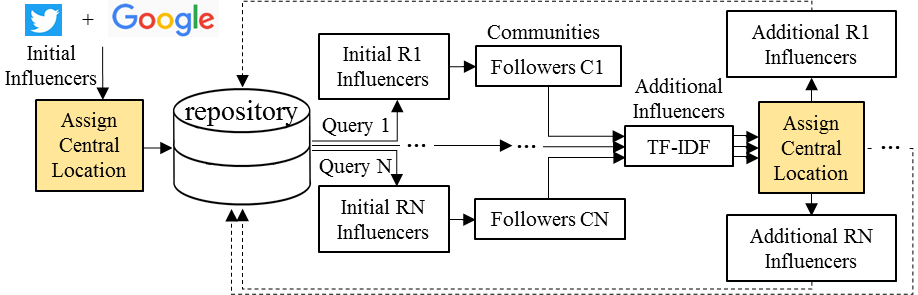
\includegraphics[width=5.4in]{fig1.png}}
\caption{Establishing and continuously updating a repository of influencers.}
\label{fig_ch4_1}
\end{figure}

Our proposed solution for building and continuously updating a repository of geo-influencers is illustrated in Fig.  \ref{fig_ch4_1}. The process extends the approach from previous chapter via the Repository and ACL process (highlighted in yellow). The required inputs are the geographic regions of interest over which influencers will be collected. A city-level location is the smallest geographic area considered since this is a popular choice among Twitter users [\ref{appendix:3.11}]. 

Larger geographical areas can be formed from cities along recognized political boundaries; cities make up fifty states, states combined into nine divisions, and divisions combined into four regions of US. Examples of system input would then be Syracuse NY vs. Buffalo NY (city), NY vs. PA (state), Mountain vs. Pacific (divisions), and Northeast vs. Midwest (regions). This section describes experiments with city and state as regions. R1 to RN geographic regions with N\textgreater1 are expected so as to be able to apply the TF-IDF measure. The main processes from Fig. \ref{fig_ch4_1} are described below:

\begin{itemize}
\item Initial Influencers: Twitter influencers from automatic Google searches related to cities making up the geographic regions.

\item Assign Central Location (ACL): the central location assigned to each influencer based on the distribution exhibited by the influencer's followers, see section 4.3. 

\item Repository: stores centroids from ACL and additional features such as percent of followers captured by the centroid, average radius, and others, see section 4.5. Repository also stores whether influencer is local or global to country of interest using classifier from Section 4.9.

\item Query: repository queried for local influencers whose C1 centroid matches the geographic region of interest. Each query can contain additional inputs such as the minimum percent of followers associated with the region. 

\item Communities and Additional Influencers: Followers of influencers from regions R1 to RN form communities C1 to CN, respectively. Influencers that these communities follow are ranked via TF-IDF. Top influencers from TF-IDF go through the ACL process and stored in the repository for future reference. 
\end{itemize}

Additional influencers refine communities associated with each geographic region and the whole process shown in Fig. \ref{fig_ch4_1} can repeat. %How the ACL process can be used to improve initial influencers coming from Google and additional influencers stemming from TF-IDF is described next. The classifier for filtering out global users described in section 4.9.

\section{Analyzing Geo-Influencers Recommended by Google}

%Initial influencers stem from automatic Google searches. %For each query, the URLs of interest are those that have the domain: `twitter.com/'. If after domain there are no backslashes, the text is used as screenname with `?lang=en' stripped out. 
%As an example, Table 4.3 shows screennames extracted from top five URLs associated with query `Syracuse, NY Twitter'. %Each extracted Twitter screenname is verified to exist on Twitter. 


\begin{table}
\small
\caption{Top Ranked URLs via Google Search for `Syracuse, NY Twitter'}
\label{table_4_3}
\begin{center}
\begin{tabular}{|c|c|c|}
\hline
\bfseries Hit & \bfseries URL & \bfseries Influencer\\
\hline
0&https://twitter.com/syracuse1848?lang=en&syracuse1848\\
\hline
1&https://twitter.com/syracuseu?lang=en&syracuseu\\
\hline
2&https://twitter.com/hashtag/syracuse?lang=en&\\
\hline
3&https://twitter.com/syracuseunews?lang=en&syracuseunews\\
\hline
4&https://twitter.com/syracusedotcom&syracusedotcom\\
\hline
\end{tabular}
\end{center}
\end{table}

Initial influencers stem from automatic Google searches. As an example, Table \ref{table_4_3} shows screennames extracted from top five URLs associated with query `Syracuse, NY Twitter'. The order of returned URLs is recorded. It was expected that the influencers extracted from first web hits will have a higher correlation to the city queried. Fig. \ref{fig_ch4_2} shows the number of influencers extracted per URL using the top 100 URLs. Queries performed across 763 city state pairs where the number of influencers per city ranged from 1 to 33. Over these cities, there were a total of 14092 influencers, 13050 remained after removing influencers associated with multiple city queries or whose followers had no location information.

\begin{figure}[htbp]
\centerline{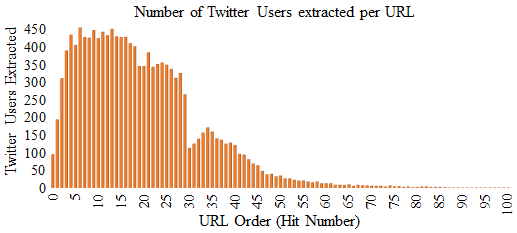
\includegraphics[width=5in]{fig2.png}}
\caption{Number of Twitter Users extracted via Google using top 100 URLs}
\label{fig_ch4_2}
\end{figure}

Next, a maximum of one million followers was collected for each influencer. Influencer's followers' self-reported locations were used to generate a distribution and compute centroids as described in Section 4.3. Error distance (\ref{eqn_ED}) computed between coordinates associated with the city queried vs. the central location coordinates from influencer's followers. Across all influencers ED@0 was 73.58\% for C1 and 70.11\% for C2. The subsections below examine the performance based on the query type, the follower sample size, and URL order.

\subsection{Performance based on Query Type}

Mean ED, Median ED, ED@0, and ED@100 were calculated across the influencers associated with each city query. Table \ref{table_4_4} shows the average and standard deviation for C1 and C2 centroids across queries. It is time consuming to analyze thousands of influencers via manual validation, but with the error measures proposed, we can quickly focus in on those queries that are problematic for Google. 

\begin{table}
\small
\caption{Average Performance across Google's Queries}
\label{table_4_4}
\begin{center}
\begin{tabular}{|c|c|c|}
\hline
\bfseries Error Measure & \bfseries C1 & \bfseries C2\\
\hline
Mean ED&53.89 +/- 164.63&63.17 +/- 150.64\\
\hline
Median ED&19.74 +/- 160.63&16.81 +/- 133.23\\
\hline
ED@0&0.69 +/- 0.32&0.66 +/- 0.29\\
\hline
ED@100&0.95 +/- 0.12&0.92 +/- 0.13\\
\hline
\end{tabular}
\end{center}
\end{table}

Out of 763 queries, only fourteen queries had ED@100 under 50\%. Thus most of Google's city-influencer associations are confirmed by the central location from influencer's followers. The problematic queries are described below.

One type of mistake stems from matching influencer not on location but based on screenname, description, or user specified name. Example of cities with human names are Lawrence MA (out of 8 influencers, city from query matched 0\% of self-reported locations, but matched 100\% of names example Jennifer Lawrence) and Anderson IN (out of 27 influencers, city from query matched 7\% of self-reported locations, but matched 96\% of names example Anderson Cooper). Contrast this to Trenton NJ where out of 27 influencers, the city from query matched 78\% of self-reported locations but matched only 52\% of names. 

Another mistake is related to state abbreviations that can be interpreted as a preposition (`OR' and `IN'). Nine out of fourteen queries faced this challenge: Gary IN, Albany OR, Anderson IN, Lafayette IN, Salem OR, Springfield OR, Gresham OR, Hillsboro OR, and Medford OR. Spelling out the state name might help these queries, i.e. Oregon instead of OR. The state name should not be spelled out for all queries because Google has more data for more common queries. For example, in the previous chapter we saw that typing out `New York, New York' causes Google's search to favor results associated with a casino in Nevada of the same name. This is again observed in that for `New York, New York Twitter' @NYNYVegas was the second URL recommended, i.e., spelling out the state name might also bring unintended results.

Finally, there were city names that are not unique to a single state. For example, there are 34 states with Springfield cities. Table \ref{table_4_5} shows specific instances where the wrong influencer was matched to query Albany OR and associated true location.

\begin{table}
\small
\caption{Google Mistakes for Query `Albany, OR Twitter'}
\label{table_4_5}
\begin{center}
\tabcolsep=0.15cm
\begin{tabular}{|c|c|}
\hline
\bfseries Albany OR Associated Influencers & \bfseries True Loc\\
\hline
albanyairport, albanysym, dutchmenpgcbl, reinventalbany &Albany, NY\\
\hline
naschoolupdates, newalbanyohio&Albany, OH\\
\hline
ahshuskies, ahuskiebaseball&Albany, MN\\
\hline
albanyassociate, albanymusicuk, thealbanyse8&UK\\
\hline
\end{tabular}
\end{center}
\end{table}

\subsection{Performance based on the follower sample size}

As described in Section 4.3 the central location is computed from influencer's followers' self-reported location distribution. For a small number of followers, there might not be enough locations to generate a proper distribution and associated centroid.

Fig. \ref{fig_ch4_3} (top) shows ED@0 error for C1 and C2 centroid as influencers with an increasing number of followers are considered. The figure illustrates that at least 500 followers are needed to get a large enough sample for computing the centroid. Because most of the influencers are associated with city level locations they, in general, cater to a smaller audience: 20\% had 500 and 54\% had 2000 followers or less.

\subsection{Performance based on Query Result Order}

First web hits have a much higher click-through rate. As a result, it was tested whether the influencers that are in the top results (low hit number) would have a higher accuracy in being associated with city query. 

Fig. \ref{fig_ch4_3} (bottom) shows ED@0 error for C1 and C2 on influencers grouped by hit number 0 to 29. Top 30 web hits were chosen because each had a good sample of Twitter influencers ranging from 387 to 490. The figure shows that the results remain about the same for influencers that appear in top vs. later web results. A possible explanation is that for ambiguous queries Google will have poor results across the board. 

\begin{figure*}[htp]
\centering
   \subfloat[Influencers grouped by number of followers]{\label{fig_ch4_3a}
      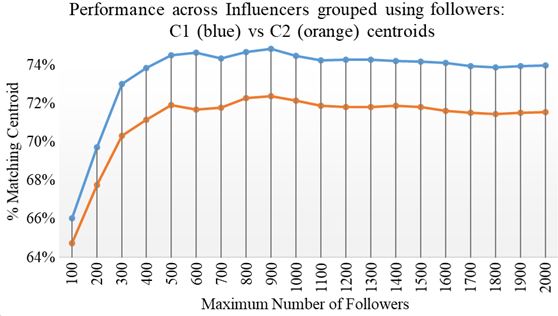
\includegraphics[width=.65\textwidth]{fig3}}
\\
   %\hspace*{\fill}   % maximize separation between the subfigures
   \subfloat[Influencers grouped by URL position from Google search]{\label{fig_ch4_3b}
      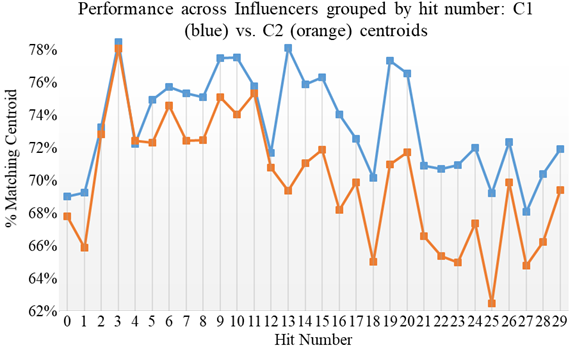
\includegraphics[width=.65\textwidth]{fig4}}
   \caption[Performance based on Follower sample size and Query order]{\textbf{Top} -- Performance based on Follower sample size. 500 or more followers provide a good sample for centroid calculation. \textbf{Bottom} -- Results from top 30 URLs illustrate that influencers in top web search results have similar performance as influencers in later web results.} \label{fig_ch4_3}
\end{figure*}

\iffalse
\begin{figure}[htbp]
\centerline{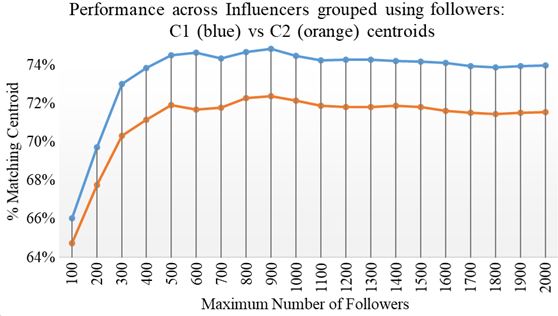
\includegraphics[width=4in]{fig3.png}}
\caption[Performance based on Follower sample size and Query order]{Performance based on Follower sample size. 500 or more followers provide a good sample for centroid calculation.}
\label{fig_ch4_3}
\end{figure}

\begin{figure}[htbp]
\centerline{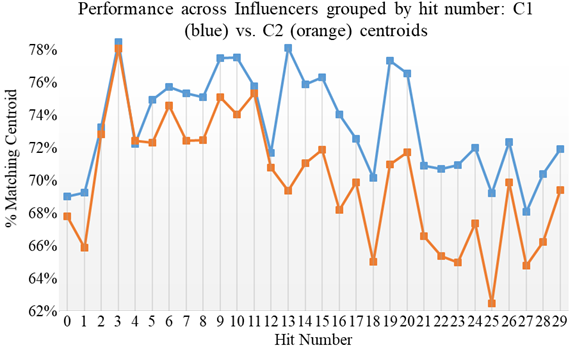
\includegraphics[width=4in]{fig4.png}}
\caption[Results based on order of top URLs]{Results from top 30 URLs illustrate that influencers in top web search results have similar performance as influencers in later web results.}
\label{fig_ch4_4}
\end{figure}
\fi

\iffalse
\section{Improving Influencers from TF-IDF}

As was shown in Fig. \ref{fig_ch4_1} the initial influencers from Google are used to form communities and discover additional influencers via TF-IDF. The dataset for this task consists of the top one-hundred influencers across 80 cities where each city was at least thirty miles away from the others and each city had at least ten Google associated influencers. Across these cities 94.33\% of initial influencers from Google had their C1 centroid match the city being queried. 7245 out of 8000 influencers remain after removing those overlapping multiple cities. A maximum of one million followers was collected for each influencer. This section examines performance based on the city and explores optimal city communities.

\subsection{Performance based on City Location}

Table \ref{table_4_6} shows cities with the least number of influencers matching the associated C1 centroid (ordered by ED@100). Salem OR and Medford OR contribute the most errors with much lower error rates for other cities. These results are unsurprising since these correspond to ambiguous Google queries discussed in Section 4.7 (errors in initial influencers from Google lead to communities that are not representative of the underlying geographical area). 

\begin{table}
\small
\caption{Ten worst performing cities using C1 centroid}
\label{table_4_6}
\begin{center}
\begin{tabular}{|c|c|c|c|c|}
\hline
\bfseries City Query & \bfseries MeanED & \bfseries MedianED & \bfseries ED@0 & \bfseries ED@100\\
\hline
Salem OR&997.34&793.38&0&0\\
\hline
Medford OR&679.98&0&0.59&0.59\\
\hline
Shreveport LA&140.03&0&0.66&0.67\\
\hline
Albany GA&102.42&0&0.76&0.77\\
\hline
Duluth MN&41.3&0&0.8&0.8\\
\hline
Dothan AL&70.51&0&0.67&0.83\\
\hline
Bismarck ND&63.5&0&0.84&0.84\\
\hline
Albany NY&116.27&0&0.85&0.86\\
\hline
Augusta GA&151.28&0&0.8&0.86\\
\hline
Salinas CA&152.98&0&0.69&0.87\\
\hline
\end{tabular}
\end{center}
\end{table}

Conversely, the top city communities had 100\% of influencers match C1 centroid (ED@0 = 0): Knoxville TN, Buffalo NY, Wichita KS, Springfield MO, Louisville KY, Syracuse NY, Boston MA, Charlotte NC, Pittsburgh PA, and Denver CO. For each of these cities, for each influencer, the city associated by Google matched the C1 centroid from influencer's followers. This again illustrates that the city communities need to be established using influencers that are confirmed by the ACL process.
\fi

\subsection{Forming Optimal Communities}

The higher the concentration of followers associated with a geographic city the better they are for establishing a city community. As an example, Table \ref{table_4_7} (top) shows five influencers recommended by Google for Syracuse, NY (each confirmed by their respective C1 centroid). Out of these @syracusedotcom has the highest concentration of followers associated with the city (70.1\%) and is thus the best for establishing the associated city community. Table \ref{table_4_7} (bottom) shows the percent of followers from Syracuse NY that follow a pair of influencers. Despite @cuse{\_}mbb having only 21.5\% of its followers from Syracuse, the table shows it can be used to improve percentages associated with followers extracted from other influencers. In this way, if a researcher wanted to focus on users from Syracuse that are interested in basketball and news, then followers of @cuse{\_}mbb and @syracusedotcom could be chosen to establish the city community with 73\% of followers mapping to Syracuse. 

\begin{table}
\small
\caption{Percent Followers mapping to City for Single vs. Pair of Geo-Influencers}
\label{table_4_7}
\begin{center}
\begin{tabular}{|c|c|c|c|c|c|}
\multicolumn{3}{c}{\bfseries Percent Followers of a single Geo-Influencers mapping to City}\\
\hline
\bfseries Influencer & \bfseries Number Followers & \bfseries \%C1\\
\hline
syracusedotcom&87334&70.13\\
\hline
sucampus&10238&53.23\\
\hline
gosyracuseu&2495&45.65\\
\hline
cuse&138595&41.63\\
\hline
cuse{\_}mbb&261805&21.49\\
\hline
\multicolumn{3}{c}{}\\
\multicolumn{3}{c}{\bfseries Mutual Followers of Two Geo-Influencers better aligned to city}\\
\hline
\bfseries Influencer Pair & \bfseries Mutual Followers & \bfseries \%C1\\
\hline
syracusedotcom + @cuse{\_}mbb&2784&73\\
\hline
sucampus + @cuse{\_}mbb&415&55\\
\hline
gosyracuseu + @cuse{\_}mbb&396&67.5\\
\hline
cuse + @cuse{\_}mbb&3250&48.7\\
\hline
\end{tabular}
\end{center}
\end{table}

A user that follows two geo-influencers has a higher chance of being from the city than the one that follows a single geo-influencer. We analyzed the percent gain over all possible pairs of influencers, where both influencers were associated by Google with the same city and confirmed by C1 centroid from the ACL process. There were 15951 pairs that produced 500 or more mutual followers across 492 cities. On average the pair had an 11.1\% gain over a single influencer. 3275 pairs had $90-98$\% percent of followers matching city of interest across 137 cities. Focusing on these pairs would lead to better city communities. It is not recommended to use three or more influencers because the overlap in followers may be too small.% (for example @cuse{\_}mbb and @syracusedotcom both have over 87K followers, but only 2.7K overlap).

\section{Classifier for City-Level Geo-Influencers}

In this section, we generate a classifier for differentiating US city-level geo-influencers vs. influencers that are from foreign countries or have more global influence. Our approach illustrates that it is possible to differentiate the two types by only geocoding the locations associated with the USA. 

Our dataset contained a total of 8740 influencers: 350 global influencers vs. 8390 US city geo-influencers. 8390 geo-influencers are obtained from Google and TF-IDF ranking. The city that the geo-influencer is associated with is verified by C1 centroid from the ACL process, the associated city name is also within the influencer's self-reported location, and each influencer had at least 500 followers (to ensure a large enough sample size as discussed in Section 4.7.2). 350 global influencers obtained via manual Twitter searches: 250 influencers are popular worldwide such as webmd, spacex, twittersports; 100 influencers came from foreign countries such as (screenname: country): ttcnotices: Canada, dailysabah: Turkey, vesti{\_}news: Russia, live{\_}hindustan: India, greateranglia: UK, and others.

Numeric features F3-F18 from Table \ref{table_4_2} were normalized to between 0 and 1 range. Nearest Neighbor (k=20), Gaussian Naïve Bayes, Decision Tree, Random Forest, and Support Vector Machines (SVM) with a linear and radial kernel were tried as classifiers with 3 fold cross validation\footnote{Scikit-Learn package utilized for implementation: https://scikit-learn.org/}. Unbalanced classes were handled by providing weights to SVM and random forest classifiers; global influencers were weighted 0.999 vs. 0.001 for city influencers (i.e. an incorrectly classified global influencer penalized classifier 1000 to 1 to ensure that all global influencers are accurately classified). We also tried to balance out the dataset by random over-sampling of the minority class. SVM and Nearest Neighbor were the only classifiers which classified all global influencers accurately. Fig. \ref{fig_ch4_5} shows average accuracy for these classifiers using an increasing number of features (drop in accuracy is due to the USA geo-influencers being classified as global/foreign) . Features ranked through Recursive Feature Elimination (RFE) with linear SVM.

\begin{figure}[htbp]
\centerline{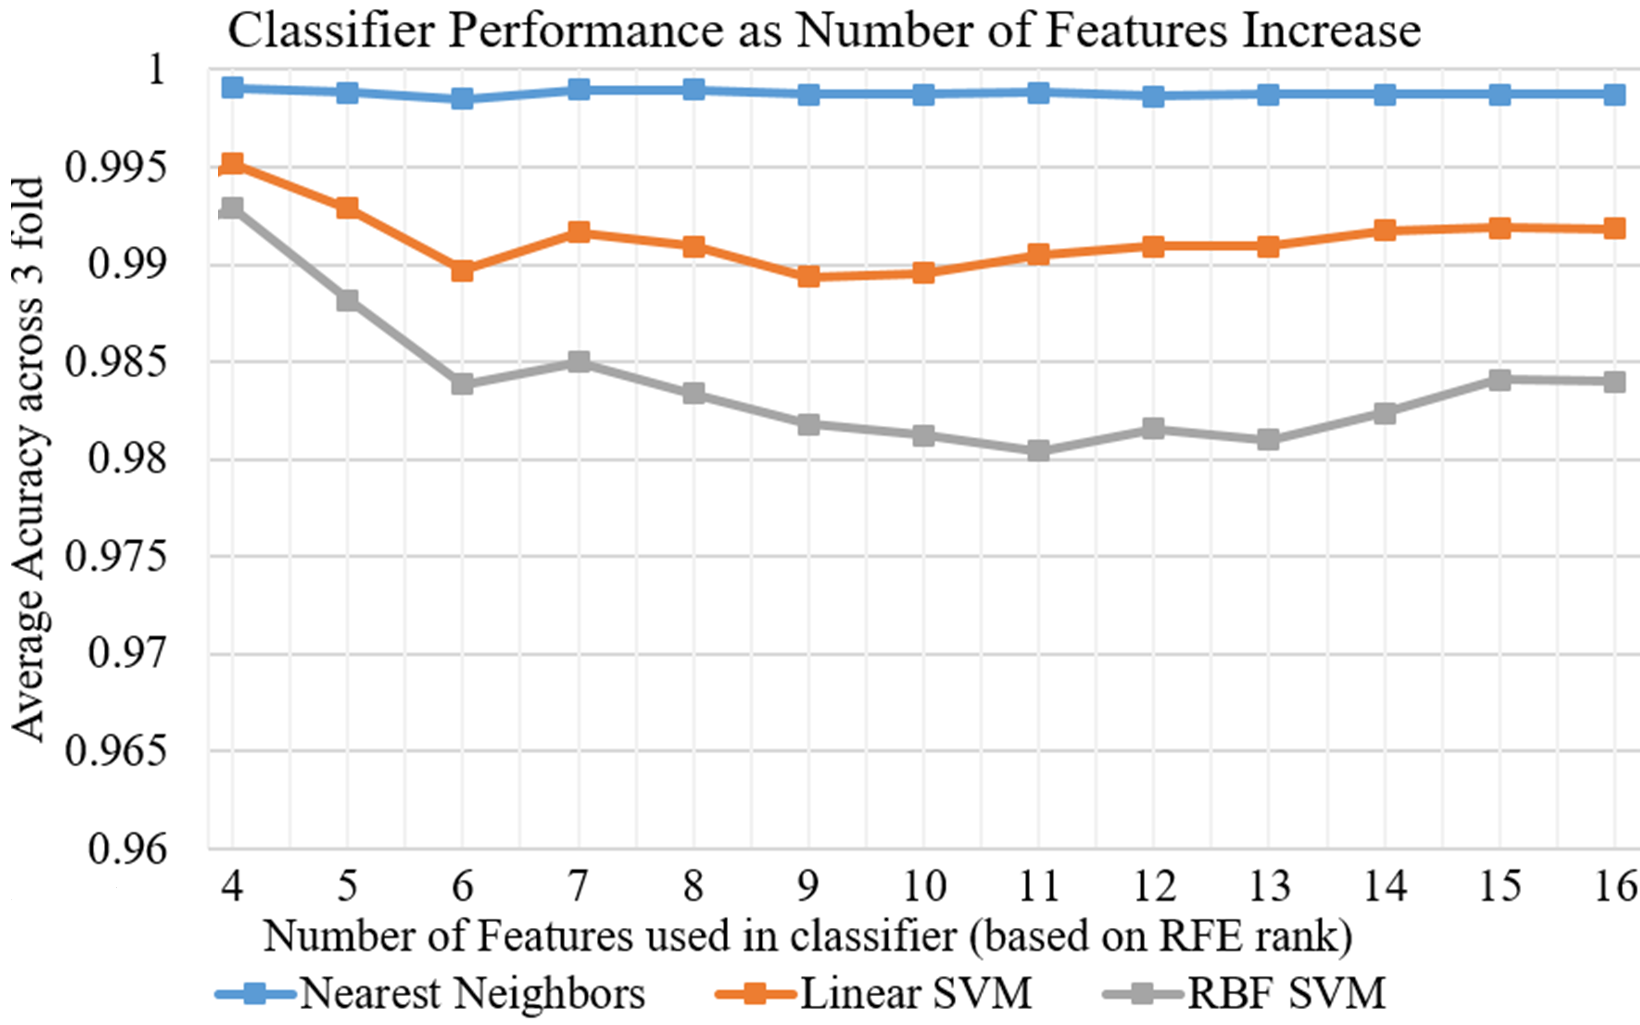
\includegraphics[width=5in]{fig5.png}}
\caption[USA vs. Foreign Country Classifier]{USA vs. Foreign Country classifier. Overall performance across three classifier peaks using top four ranked features.}
\label{fig_ch4_5}
\end{figure}

All three classifiers have peak performance when using the top four ranked features: F8 (percent followers mapping to US distribution), F13 (ratio of followers from sample mapping to C1 centroid), F7 (number of followers to US distribution), and F3 (distance between C1 and C2). Classifier performance using these four features illustrates that it is possible to differentiate US city vs. global influencers without having to geocode locations outside of the USA.

The results are intuitive in that influencers associated with a city $c$ in a country $x$ should (i) have a higher overall concentration of followers going to this country $x$ (necessary for filtering out influencers associated with foreign countries) and (ii) should exhibit an above average concentration of followers associated with the specific city $c$ (necessary for filtering out global influencers that may have a high concentration of followers in country x but whose influence spreads over many cities).

These are important results to consider because geocoding locations all around the world is difficult. For a specific country of interest, our recommendation is to focus on well-known cities within this country for forming a frequency distribution as was described in section 4.3. City influencers can then be extracted using a classifier and by focusing on those influencers verified by the C1 centroid. As the repository continues to grow in size the classifiers are expected to continue improving.

\section{Conclusions}
Our research proposed an automated evaluation for a targeted collection of influencers and corresponding city-level communities. The approach, described in this chapter, should be applied to verify that the geo-influencers and the resulting city-level communities for the USA from chapter 3 are accurate. 

The evaluation showed that Google does occasionally make mistakes for queries involving ambiguous city names (those that appear along with multiple states or that match popular human concepts). Our evaluation process allowed us to quickly identify these errors without having to review thousands of influencers manually. Queries with fewer than 50\% of influencers within 100 miles of the expected centroid (ED@100) were manually verified to be challenging for Google. The performance was about the same for influencers in top vs. later web results, i.e. web hit number does not play a significant role in how well influencer is associated with city query. Finally, it was shown that at least 500 followers are needed to have a large enough sample from which to compute the central location.

The method allowed to automate an evaluation covering thousands of influencers. Larger geographical areas were specified by aggregating multiple cities for a state-level evaluation. It was also illustrated how multiple influencers with a geographically local audience could be used to form city communities better aligned to the location of interest. Finally, a classifier was proposed for differentiating the USA vs. global and non-USA influencers; this classifier is possible without a geocoder dedicated to other languages. 

The methods described here are useful for generating and maintaining a repository of city-level influencers for the USA or other English-speaking countries (this is because the evaluation is still reliant on a gecoder that can process English-based locations). In the next chapter, we describe an approach that works worldwide by categorizing influencers using time-based features.

\iffalse
\subsection{Summary}

This section showed that Google does occasionally make mistakes for queries involving ambiguous city names (those that appear along with multiple states or that match popular human concepts). Our evaluation process allowed us to quickly identify these errors without having to review thousands of influencers manually. Queries with fewer than 50\% of influencers within 100 miles of the expected centroid (ED@100) were manually verified to be challenging for Google. The performance was about the same for influencers in top vs. later web results, i.e. web hit number does not play a significant role in how well influencer is associated with city query. Finally, it was shown that at least 500 followers are needed to have a large enough sample from which to compute the central location.
 
In general, if the query is unambiguous Google will do an excellent job in associating location-aware influencers with the city level location they serve, but Google cannot be always assumed correct. We improve the approach from reference [\ref{appendix:3.3}] by removing each influencer $u$ whose associated location is not confirmed by C1($u$) (2).
\fi
\graphicspath{{Figures/}}
\chapter{Inferring Degree of Localization and Popularity of Twitter Topics and Persons using Temporal Features}\label{chap5}

\setlength{\abovedisplayskip}{-20pt} \setlength{\abovedisplayshortskip}{-15pt}

\section{Introduction}

%Identifying authoritative users (experts) or influencers on social networks is an important topic of research\footnote{We use the term influencer and expert interchangeably when referring to an authoritative user}. Local expert finding is important for many applications such as answering local information needs. The area of influence and expertise may be localized within a small geographical area for some influencers, and be much broader for others. 

 %The problem with local expert finding in social networks and on Twitter, in particular, is the lack of geo-information. Less than 1\% of message traffic contains geo-information, and available information about a user's location is limited to a self-reported textual field that may not be filled in. 
 
 Previous chapters have focused on improving geocoding and leveraging Google search for associating influencer with a city. In this chapter, we illustrate an alternative approach for how the creation times can be used to infer geo-information. 
 
 On Twitter, every user and every message has a creation timestamp. For a group of users or a group of messages, the creation times can be used %for understanding
 to help determine whether the group is concentrated in a single time zone or is spread out more globally. The Coordinated Universal Time (UTC) offset\footnote{UTC is the time standard used globally, defined by the International Telecommunication Union Recommendation (ITU-R TF.460-6); it is a refinement of previous time standards such as Greenwich Mean Time. For instance, the UTC offset is -5 for the time zone that includes the northeastern USA.} 
 can be identified for a group that is from a specific time zone. For a global group (such as the followers of a global influencer), the daily changes in followers can be inferred and used for studying the influencer's evolving popularity.
 
 The time-based features discussed have applications related to (i) local expert finding in social networks, (ii) inferring when followers joined an influencer, and (iii) understanding popular trending topics from message traffic relevant to a specific geographic area. The methods in this paper maintain user's privacy because the location inference is at the timezone level. 
 
When performing Twitter data collection need to consider Twitterbots, a software program that sends out automated posts on Twitter [\ref{appendix:2.27}]. There are malicious and benign bots. Malicious bots threaten the security of other users [\ref{appendix:bookCh2.1}] by posting malicious URLs along with hot trending topics [\ref{appendix:bookCh2.2}]. Such accounts are actively being blocked by Twitter. Examples of benign bots are job postings, weather, news, and traffic updates. Such bots do not violate the rules of Twitter and are allowed to operate. The issue is that the bots can generate a lot of message traffic compared to real users. For example, Tasse et al. [\ref{appendix:1.13}] find that job-posting bots constitute a growing portion of the public geotags. For analysis over message traffic, to reduce the impact of bots, it is recommended to focus on a single, most recent, message per user. For analysis over influencer’s followers, it is recommended to consider each follower's tweet frequency (number of messages posted by follower divided by the number of days elapsed since account creation). Our analysis is focused on influencers that have been verified by Twitter to be legitimate but in general followers-friends ratio, tweet frequency, number of times added to favorites, and other features such as screen name length are used for identifying real influencers [\ref{appendix:bookCh2.3}].

The rest of the chapter is structured as follows. Section \ref{sec2} reviews prior research related to local expert finding. Section \ref{sec3} shows how group creation times can be used in a time distribution and how this distribution can be used for predicting the UTC offset. Section \ref{sec4} analyzes the 
temporal distribution of message traffic.
Section \ref{sec5} analyzes the variations in the number of followers and illustrates how those can be used for understanding daily followers gained. This is useful for link inference and understanding evolving popularity of global influencers. Section \ref{sec6} describes a classifier for the discrimination of local vs. global influencers. Finally, Section \ref{sec7} presents our conclusions and future research directions.

\section{Related Research} \label{sec2}

The problem of finding authoritative users is known as expert finding; this is a well-studied problem with research going back over a decade, and has gained popularity within the information retrieval community since it was included in the TREC enterprise track [\ref{appendix:bookCh2}]. A recent survey by Husain et al. [\ref{appendix:bookCh3}] reports that a majority of the expert finding systems were used in: (i) the academic domain (research collaborations), (ii) enterprise (experts for offering formal help related to development), (iii) medicine (medical experts), (iv) online knowledge sharing communities, (v) online forums, and (vi) social media (finding experts from various social networks like Twitter and Facebook).

Expert finding methods assume that individuals' published documents are relevant to their expertise with different degrees of a match, and they focus on modeling the associations between these documents and candidate experts.

%Our research deals with social networks. 
Lappas et al. [\ref{appendix:bookCh4}] give an early survey on expert finding in social networks, which typically involves (i) using text content posted by expert candidates and (ii) using the expert candidates' online social connections. Two best-known algorithms that exploit link structure to find authorities are based on PageRank [\ref{appendix:bookCh5}] and  Hyperlink-Induced Topic Search (HITS) [\ref{appendix:bookCh6}]. 

Weng et al. [\ref{appendix:2.24}] proposed TwitterRank which employs the Latent Dirichlet Allocation (LDA) model to detect the topics of individuals based on their tweets. Then, for each topic, it builds a weighted graph based on the topical similarity between two users %and their follower graphs 
and then employs a PageRank algorithm to find topic-specific influential users. 

Romero et al. [\ref{appendix:bookCh8}] designed an algorithm similar to HITS named Influence Passivity algorithm to quantify the influence of users in a Twitter network. This algorithm utilizes both the structural properties of the network as well as the diffusion behavior among users. Pal et al. [\ref{appendix:bookCh9}] proposed an attribute-based approach for identifying experts and potential experts in community question answering. Fifteen features were extracted from the Twitter graph and tweets posted by the users, to estimate their levels of expertise on various topics. 
Clustering (based on the Gaussian mixture model) was used to determine experts,  maximizing the likelihood of the data given a number of Gaussian components.

Ghosh et al. [\ref{appendix:bookCh10}] proposed a system called Cognos, which represents each user by the metadata of Twitter lists that contain the user, then ranks users based on %employs a similarity measure to compute 
the similarity score between each user and a topical query.
%, which is used to rank users for search. 
Cognos tends to choose users that are contained in many lists and whose metadata contains the query. The authors show that their system can identify top users for a particular topic better than graph based approaches. 

%In literature there is differentiation between topical and location-aware experts. 
Separately, research efforts have addressed the task of finding local experts %differ from general topic experts in that they have 
with specialized knowledge focused around a particular location. Local experts are important for many applications such as answering local information needs [\ref{appendix:bookCh11}]. 

Li et al. [\ref{appendix:bookCh15}] proposed applying points of interest (POI) as a possible categorization of expertise related to a particular geographic location. Example `Chinese Restaurants' in Los Angeles is a POI topic. High-ranking candidates should be able to answer questions about the locations or the category of locations in the topic. The time user reported being at a POI is seen as an important feature in that frequent visits result in greater familiarity with the location in question [\ref{appendix:bookCh16}]. 

Niu  et  al.  [\ref{appendix:bookCh17}]  introduced  a  learning-based  method  to find  local  experts  on  Twitter.  They  defined  multiple  classes  of features that could impact a user's local expertise, such as tweet content  features  (e.g.  the  TF-IDF  score  of  a topic  keyword  in  the candidate's tweets) and local authority features  (e.g. the  distance between the candidate and the query location). Authors found it best to  retain only the first check-in during a repeated activity (a user posting multiple times about a newly served dish during the same meal is an example of the same venue during which the user remains in an unchanged location and activity). 

A recent review by Yochum et al. [\ref{appendix:bookChNew3}] analyzes systems that recommend items (such as venues, places, travel routes, activities, friends, or social media) to users while considering geographical preferences. They analyzed 178 journal papers in this area from 2001 to 2018. They found that Foursquare, Gowalla, Brightkite are popular social media sites since these are Location-based Social Networks (LBSNs). LBSN websites are where users share their locations by checking-in so there is no need to geocode, geoparse or geotag. Twitter used in about 4.5\% of publications vs. 46.6\% over these three LBSN sites. Twitter is typically used for getting the popularity of points of interest or locations by extracting from messages with coordinates: (i) construct an ordered sequence of relevant text; (ii) map to the popular points of interest using latitude and longitude; and (iii) generate time sequences of point of interest visits. 

Several research papers rely on geotagged tweets or text-based Location Indicative Words (LIW). Singh et. al. [\ref{appendix:bookChNew7}] focused on tweets with GPS coordinates that contained the words ‘flood’, ‘water’, and ‘Baarh’ for flood event detection. Luceri et. al. [\ref{appendix:bookChNew4}] propose a deep learning architecture that aims to infer the geo-tag of a generic user’s tweet by leveraging the geo-tags shared by other users on Twitter. This work is similar to inferring a user’s location based on friends’ self-reported locations [\ref{appendix:1.11}], but instead of using self-reported locations, it focuses on those friends that have generated a message with precise coordinates. To preserve privacy, the authors recommend either to stop producing messages with geo-tags or to purposely alter the geoinformation so that it is outside of the user’s actual location. Paule et. al. [\ref{appendix:bookChNew8}] perform geotagging of tweets using weighted majority voting of geotagged tweets whose content is most similar. This increases available geotagged tweets with improved performance demonstrated in New York and Chicago. In papers that attempt to identify topical experts typically the GPS coordinates and place mentions associated with messages are utilized. Inkpen et al. [\ref{appendix:bookCh23}] develop a city, province, and country classifier for monitoring places mentioned in Twitter messages.

The issue with focusing only on tweets with GPS coordinates or POI information is that they make up a small portion of the Twitter API stream [\ref{appendix:1.1}, \ref{appendix:1.8}]. Geocoding the message's author self-reported location is complicated. Jurgens et al. [\ref{appendix:1.8}] reported that using popular gazetteer solutions GeoNames, DBPedia, GeoLite, and Google's geocoder were able to each geocode under 4\% of users using self-reported location [\ref{appendix:1.8}]. %For users whose location cannot be extracted from their message or profile information, the median location of the user's friends may be used [\ref{appendix:3.13}]. 

%Wei et al. [\ref{appendix:2.26}] attempt to identify local influencers across three US cities using several modified PageRank based algorithms. Their network was built using social activity based interactions retweet, reply, and mention present in over five billion tweets (message contents not analyzed). The influencer's self-reported location was used for filtering out those influencers that are not from the area such as \emph{@YouTube}. However, it was also shown that limiting users within x miles of the location of interest would filter out other important users, that had a strong local connection spanning beyond 100 km.

Multiple surveys have been written related to Twitter user geolocation [\ref{appendix:1.1}, \ref{appendix:1.8}]. Jurgens et al. [\ref{appendix:1.8}] reimplemented some of the state-of-the-art models, tested and trained them using their own constructed dataset to ensure fairness of comparison, and found significant performance issues. Mourad et al. [\ref{appendix:bookCh13}] proposed a guide for a standardized evaluation of Twitter user geolocation. Analysis of fifteen models and two baselines illustrated that the choice of effectiveness metric can lead to diverging conclusions. Due to the high levels of noise and the data collection restrictions imposed by the Twitter API the user geolocation remains an unsolved research area. 

Other features useful for identifying locations are the time zone and UTC offset [\ref{appendix:6b.14}, \ref{appendix:6b.15}]. Zannettou, et al. [\ref{appendix:6b.16}] used time zone information to understand the  audience targeted
by tweets from Russian-linked accounts. But due to privacy reasons, Twitter has made these fields inaccessible in 2018. 
%Recently, Panasyuk et al. [\ref{appendix:1}] 

%Related to time, 
\newcommand{\datetime}{time information }
Twitter does not keep track of any time information other than identifying when a user or a message was created. Data for link creation times between users and their followers are not stored, although it can be extracted by performing multiple scans of the Twitter network. For example, Kwak et al. [\ref{appendix:5.16}] collected daily snapshots of the online relationships of 1.2 million Korean-speaking users for 51 days as well as all of their tweets to estimate popularity dynamics.

This research proposes new time-based features based on user and message creation times. Creation times over influencer's followers are used for predicting the time zone's UTC offset and associated geographic area that the followers belong to. When applied over message traffic, the approach can differentiate top trending topics and persons in different geographical regions. The degree of localization (``localness") is %a difficult concept for which there is still not a consensus definition 
an important concept, with ongoing work in formalizing the notion [\ref{appendix:3.15}]. Our time-based features are successfully applied in a classifier for predicting local vs. global influencers. The resulting classifier can be applied as a post-processing step for verifying that the local expert is indeed local. The new time-based features are not just limited to inferring location, but can also be used for inferring link creation times for studying the evolution of influencer's popularity.

\section{UTC Offset Prediction based on Account Creation} \label{sec3}

This section describes how the time zone's UTC offset is predicted from a set of creation times. The creation times can come from a set of users or a set of messages. Subsection \ref{subsec-UTCdata} describes the dataset; the creation times come from a group of users whose self-reported location is in common and where the location's UTC is known. Subsection \ref{subsec-UTC} describes %the approach for
how a time distribution is formed and how it is used to predict the UTC offset. Subsection \ref{parameterDeter} describes experiments %that was used
to find the optimal parameter values used in the proposed approach.

%In Section \ref{subsec-UTC}, we present the process used for generating UTC information.  
%Section \ref{subsec-illustration} illustrates how message traffic distributions are identified and used in our analysis. \textbf{This sentence belongs to Section 4 (unless you decide to put both in the same Section 3. You may want to use sub-sub-section format)}

\subsection{UTC Offset Dataset} \label{subsec-UTCdata}

Over 373 million user profiles were analyzed and user groups were chosen based on self-reported location in common. All self-reported locations were turned to lowercase with punctuation and spacing stripped out. Of particular interest are those self-reported locations that match (i) (City, Province) or (ii) (City, Country Name) in English from GeoNames. The city, country pairs are checked to be unique in that there are no other cities within the country with the same city name. The population of all cities considered in is over five thousand. Major well-known city names are included (without the country name) provided the city is unique and has a population of over 1 million. Each self-reported location had to be used by at least 250 unique users to ensure a large enough sample size. %\textbf{to ensure a large enough sample size for generating the normalized time histogram. Too early to talk about normalized time histogram.} 
 
 %\textbf{Table 1 below provides some good examples but useless otherwise. Do we use this information anywhere in the following?} \textbf{london and losangeles used in Fig 1)
 
The resulting dataset, % so constructed,
denoted $D_{UTC}$, consists of 12,271 groups. Table \ref{table_0} shows the five most popular locations, the number of users making up each group that use the location, and the UTC offset associated with the location, denoted as $UTC^L$, using equation (\ref{eq00}).

\begin{equation}
UTC^L(loc) = \frac{1}{3}UTC(tmz(loc))+\frac{2}{3}DST(tmz(loc))\label{eq00}
\end{equation}

%In equation (\ref{eq00}), 
GeoNames is used to get the location's time zone\footnote{download.geonames.org/export/dump/timeZones.txt} via function \textit{tmz}. UTC and DST functions are used to obtain the UTC offset %observed %at time zone 
during standard and daylight saving time, respectively; these are equal in time zones where daylight saving is not observed.
%UTC and DST produce equal offset). 
Daylight saving time is typically observed for eight months of the year and is thus given a larger weight.



In our dataset, $UTC^L$ takes 42 possible values ranging from -9.9 to 13.53. Therefore, the corresponding UTC offset interval for our dataset is [-10, 14) (UTC offset -12 and -11 exist, but belong to sparsely populated islands and therefore not of interest).  Table \ref{table_0} describes the attributes of the five largest user groups in the dataset.

\begin{table}[htbp]
\small
\caption{Five biggest user groups in UTC Offset Dataset}
\label{table_0}
\centering
\begin{tabular}{|c|c|c|c|}
\hline
\bfseries Location & \bfseries Group Size & \bfseries UTC\textsuperscript{L} & \bfseries Country \\
\hline
london & 2065562 & 0.667 & GBR \\
\hline
losangelesca & 1768898 & -7.333 & USA \\
\hline
newyorkny & 1425330 & -4.333 & USA \\
\hline
chicagoil & 1173340 & -5.333 & USA \\
\hline
parisfrance & 1026459 & 1.667 & FRA \\
\hline
%{atlantaga & 783997 & -4.62 & USA \\
%{\hline
%{houstontx & 744874 & -5.61 & USA \\
%{\hline
%{newyorkusa & 739374 & -4.62 & USA \\
%{\hline
%{sanfranciscoca & 702652 & -7.59 & USA \\
%{\hline
%{bostonma & 666833 & -4.62 & USA \\
%{\hline
\end{tabular}
\end{table}

\subsection{Sleep Cycle and UTC offset Determination} \label{subsec-UTC} %High Level Approach}

The following procedure is used to identify the UTC offset in the geographic area from which the creation times originate. Given a set of creation times:

\begin{enumerate}
\item Creation times to Time Distribution:
\begin{enumerate}
    \item 
The hour from each creation time is used to generate a histogram, with 24 bins corresponding to 24 hours. 
\item 
Time distribution refers to a normalized histogram; $f(t)$ used to denote the relative frequency of creation times within $t^{th}$ hour. 
\end{enumerate}
\item Preprocessing:
\begin{enumerate}
    \item 
The 24-hour time distribution is duplicated to generate a 48-hour distribution.
\item The distribution is smoothed by computing the moving average of $n=5$ consecutive points.%, for different values of $n$.
\end{enumerate}
\item Sleep cycle identification:
\begin{enumerate}
    \item 
If there are four intersection points (between $f(t)$ and the $p=33$ percentile),
per 48 hours, the sleep cycle is identified as a single continuous segment between  
%\item The start and end of the sleep cycle are 
two consecutive intersection points where the first has a negative and the second a positive slope. %, respectively.
\item A quadratic %polynomial 
function is fitted over sleep cycle: $f(t) = c_0 + c_1\times t + c_2 \times t^2$. %If it is a U-shaped parabola than the minimum of the parabola is recorded. This
If $c_2 > 0$, its minimum is considered to be the group's \textit{Potential Sleep Time (PST)}, subtracting 24 if needed, so that PST $\in [ 0, 24)$. 
\end{enumerate}
\item UTC offset computation:
\begin{enumerate}
    \item 
Given a PST $\geq$ 14 the               transformation PST-24 is applied to transform  PST from [0, 24) range to the UTC range [-10, +14).
\item 
Linear regression on known data is used to express the UTC offset as a linear function of PST, using Equation (\ref{eq001}) at the end of this section based on Fig. \ref{fig_3}.
%$UTC^P = -1*PST + 4$; using equation (\ref{eq001})
\end{enumerate}
\end{enumerate}

\begin{figure*}[htp]
   \subfloat[self-reported location `london']{\label{fig_1a}
      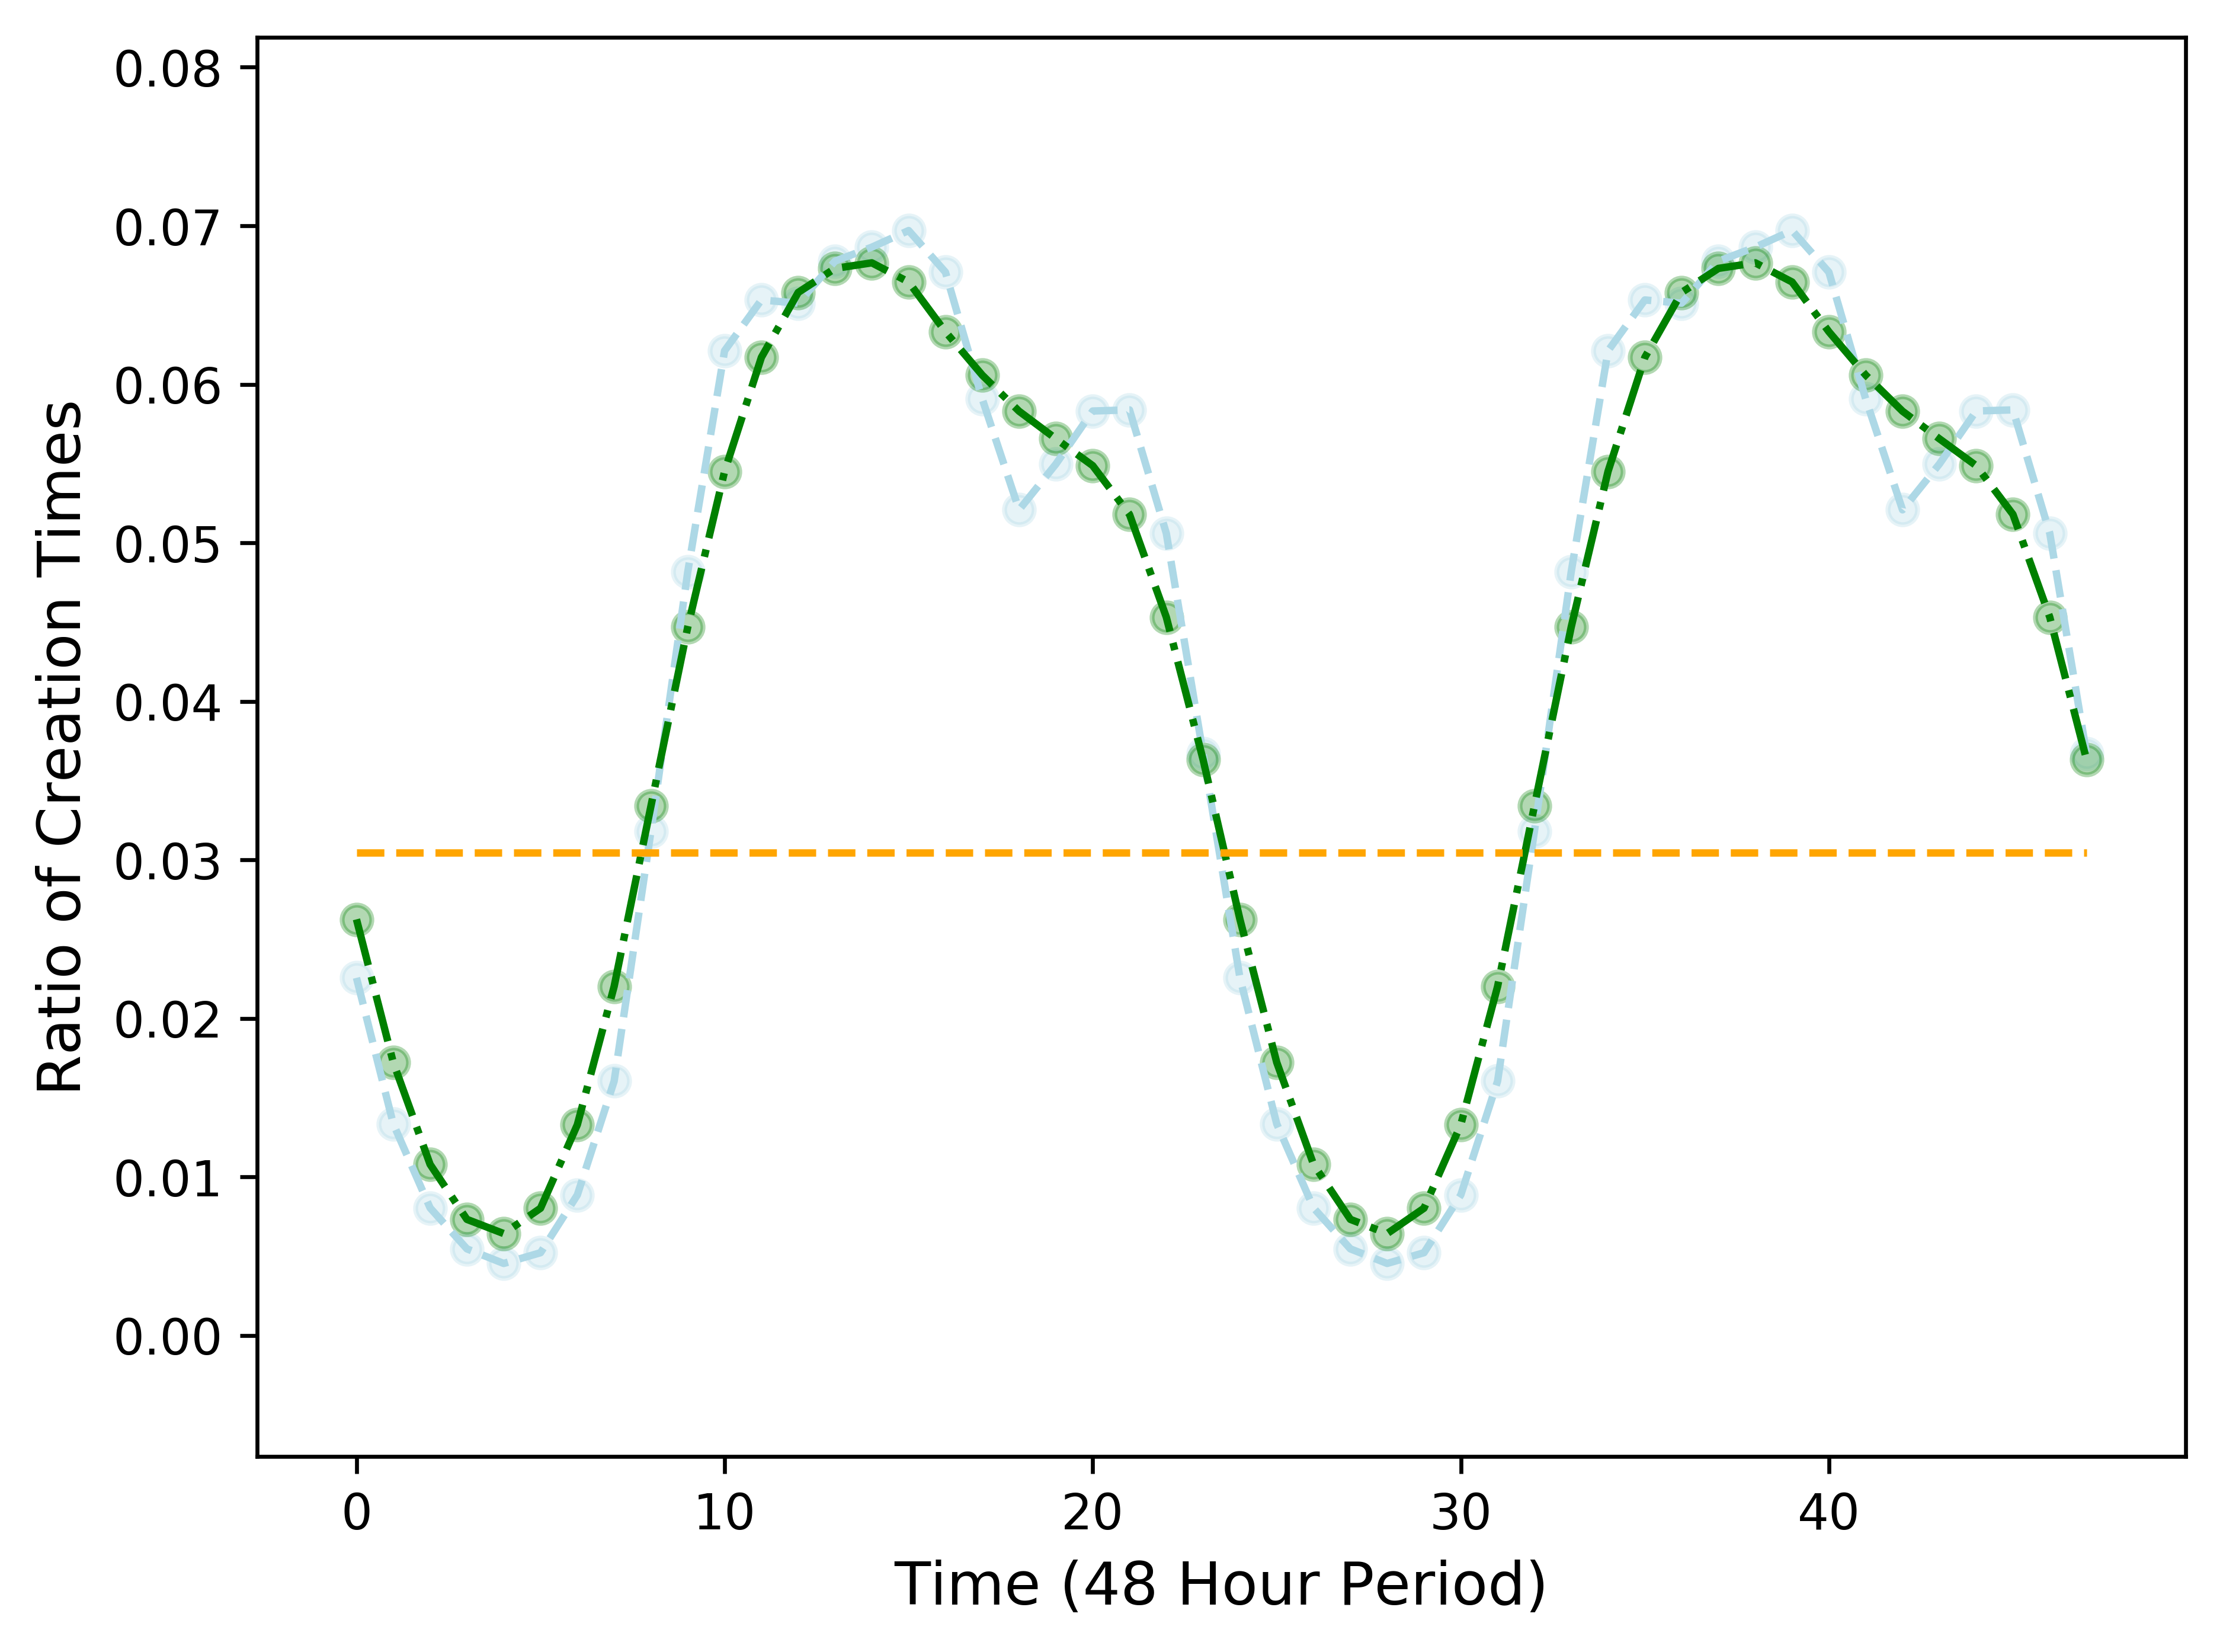
\includegraphics[width=.48\textwidth]{Figures/london.png}}
   \hspace*{\fill}   % maximize separation between the subfigures
   \subfloat[self-reported location `losangelesca']{\label{fig_1b}
      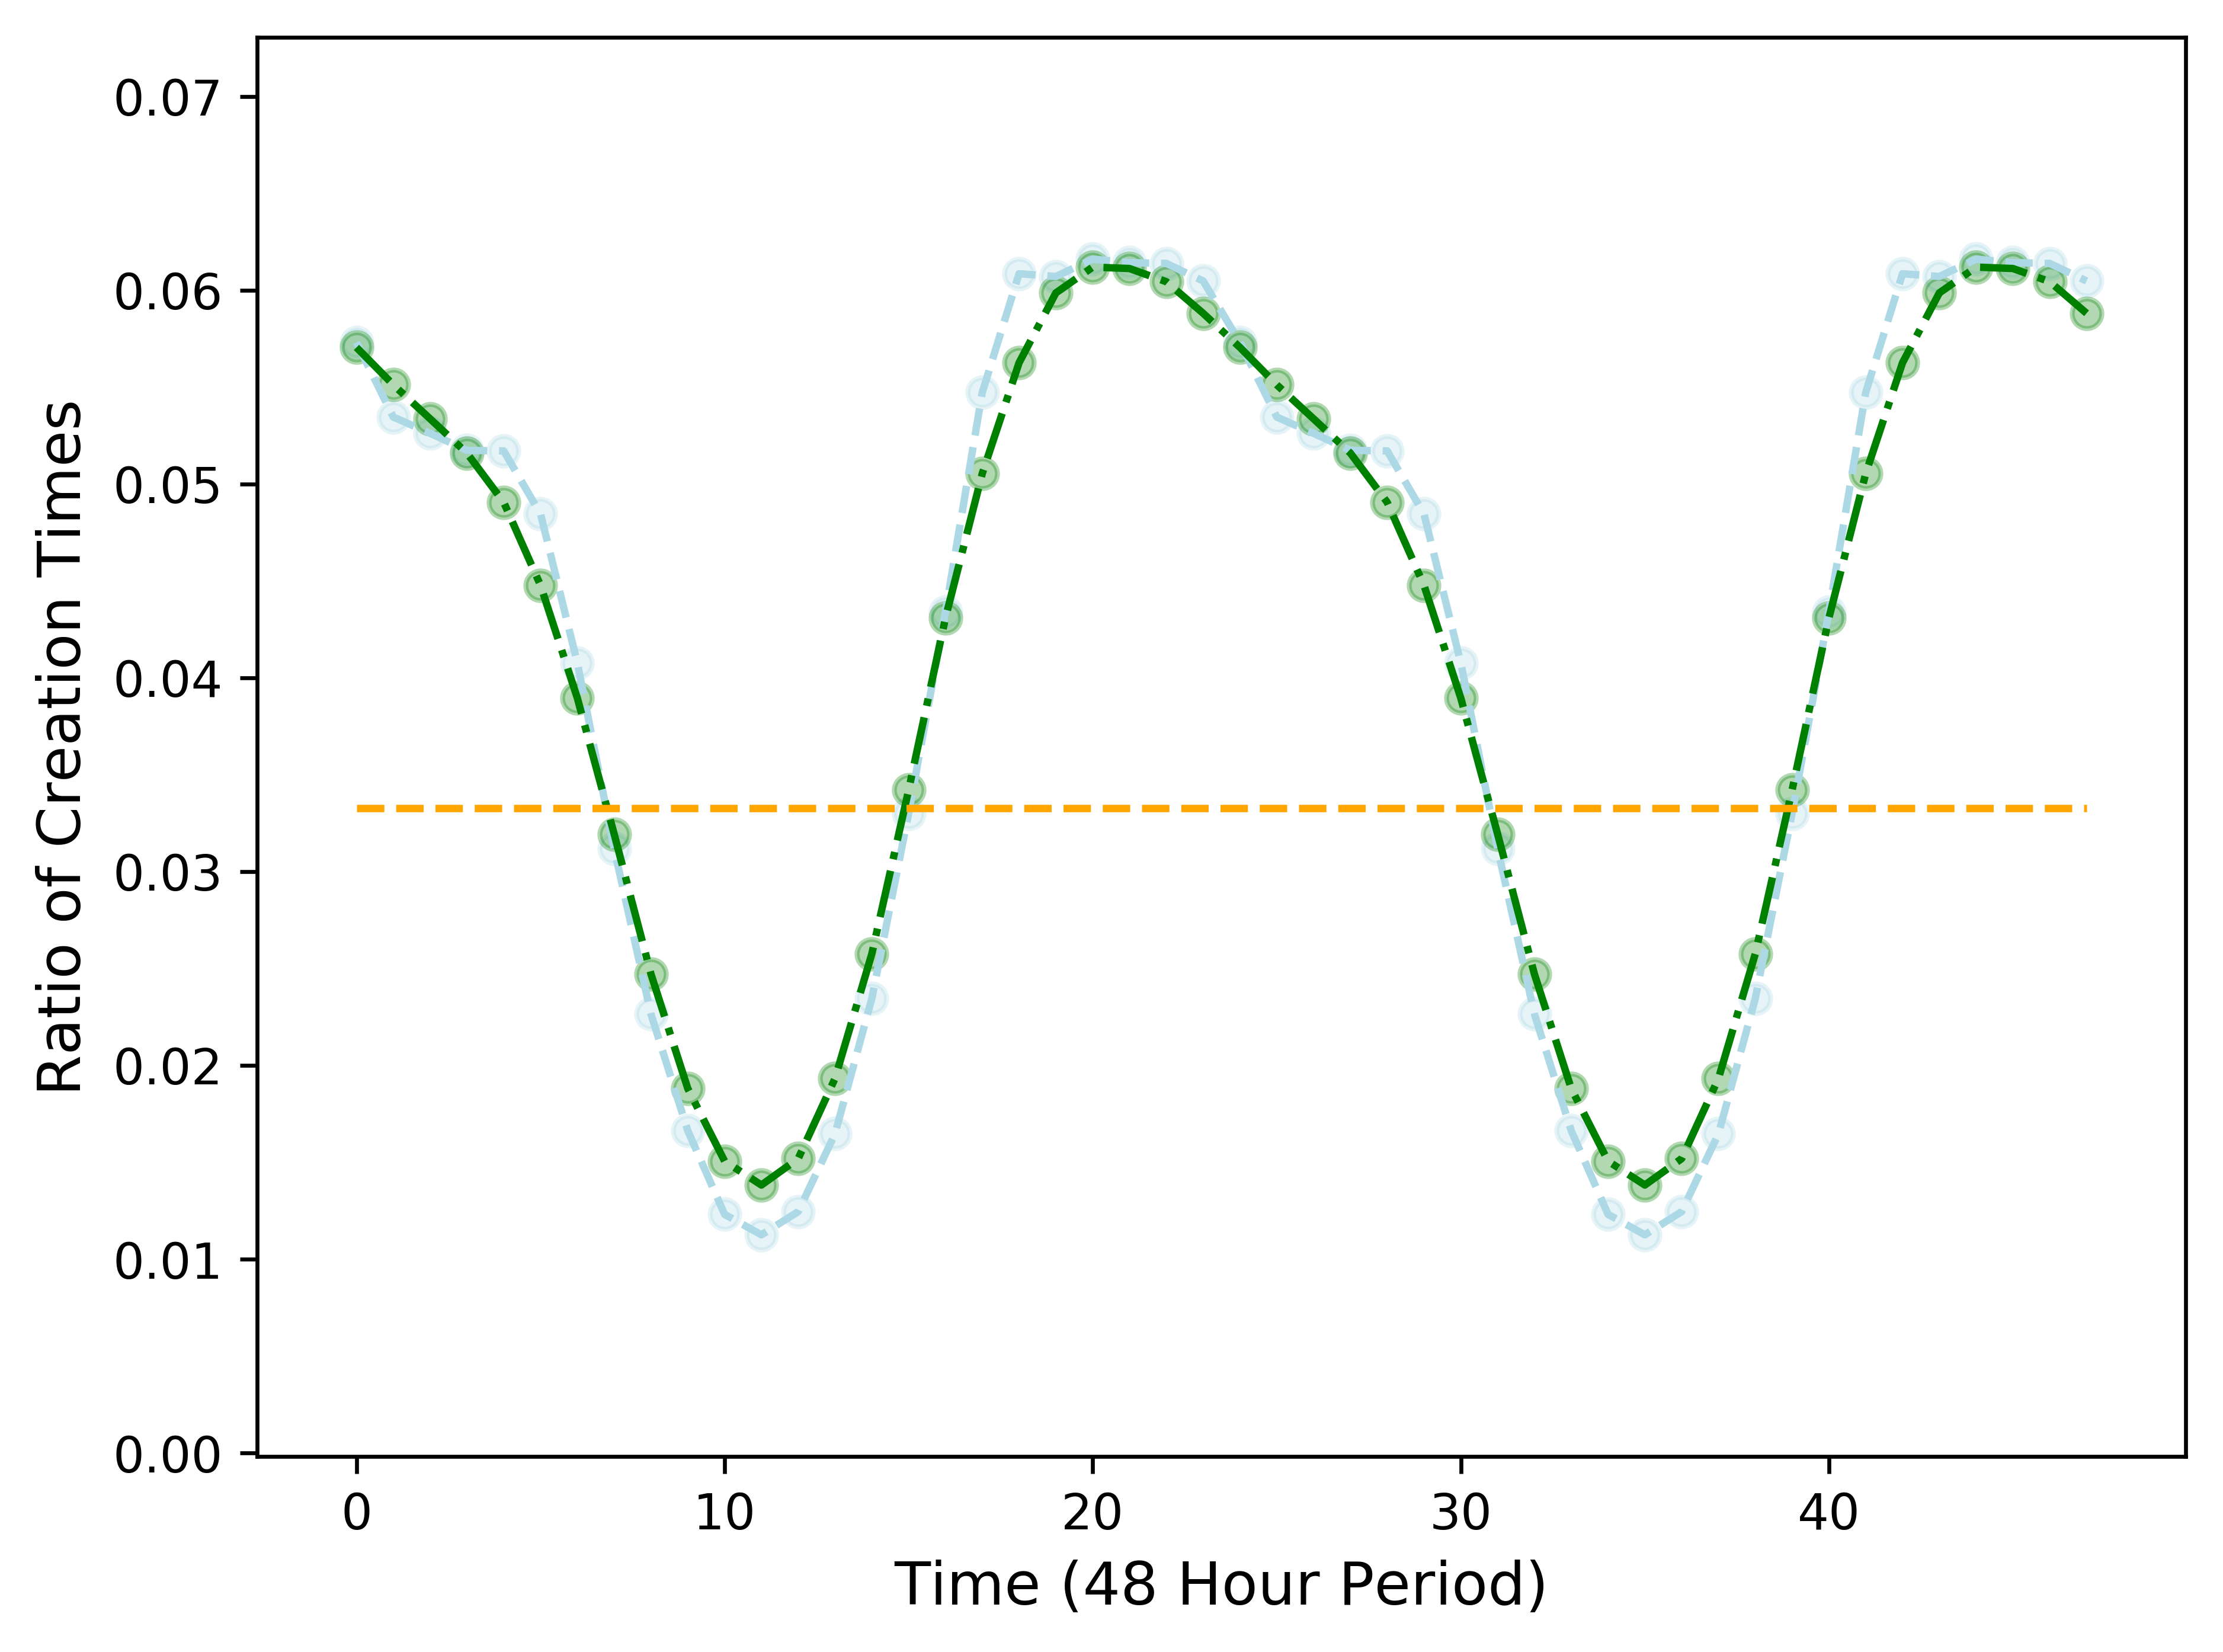
\includegraphics[width=.48\textwidth]{Figures/losangelesca.png}}
   \caption[Example Time Distributions]{Normalized 48-hour histograms using creation times of users from (a) `london' and (b) `losangelesca' are shown. The blue curve shows the original time distribution, and the green curve represents the moving average (with $n=5$). The orange line corresponds to the threshold below which the potential sleep cycle is identified from the green curve. The mins between the two charts are 7-9 hours apart matching expectation in that the time difference between the two locations is 8 hours.} \label{fig_1}
\end{figure*}

As an illustration, Fig. \ref{fig_1} shows the $f(t)$ formed from creation times corresponding to users associated with %that use 
locations (a) `london' and (b) `losangelesca'. %The $f(t)$ may be uneven, see blue lines in Fig. \ref{fig_1}, 
The data (%shown with 
blue lines) is noisy, and to achieve smoothness we compute moving averages (with $n=5$ consecutive points), % moving average which are 
depicted by green lines.% in the figure. % and clearly they are much smoother. 
The orange line corresponds to the threshold below which the potential sleep cycle is identified from the green curve.

%User group or message traffic that is originating from a specific time zone will result in a time distribution that has a U-shaped parabola. The U-shaped parabola 
It is assumed that the regions around the minima (in the smoothed curve) correspond to 
a nocturnal period when many residents of the region sleep, and hence are not active on social media.
%corresponds to the night time in the specific time zone and for this reason there is less activity. 
This region, expected to be an 8-hour period (a third of the 24-hour cycle) % is expected to be devoted to sleep. The sleep portion of the 24-hour cycle can be 
is identified using the threshold %of  $f(t)$ %is below the percentile
$p=33\%$ in Fig. \ref{fig_1}). 
%The sleep cycle %for bottom chart
%occurs between %the first and second intersection points of this threshold.
%and for top it is between the second and third intersection points. 
The portion of the smoothed curve below the threshold can be approximated by a quadratic function. Minimum of the quadratic used to predict the UTC offset; confidence in which increases with the coefficient of determination $R^2$ and the magnitude of the power coefficient $c_2$ ($c_2$ close to zero associated with a flat like sleep cycle with not as clear a minimum).
% function %and if it is a U-shaped parabola to make a UTC prediction. 
We record (i) the predicted UTC offset, (ii) the power coefficient $c_2$,  and (iii) the coefficient of determination $R^2$.

The next subsection addresses the selection of  parameters for the moving average $n$ and the percentile $p$ threshold,
and describes the linear regression leading to the computation of UTC.
%work the best and how the e
%Equation (\ref{eq001}).

\subsection{Parameter Determination} \label{parameterDeter} 

Instead of using the entire $|G|$ creation times of the group, we use a method akin to bootstrapping %(see Efron and Tibshirani~
[\ref{appendix:bookCh28}]). Random samples of size $M$ are drawn from $G$, $N$ times, and for each sample, the PST is calculated. 
Over $N$ trials, the average PST is denoted $\mu_G({PST})$, 
and $\sigma_G({PST})$ denotes the standard deviation. %of PSTs over $N$ samples is calculated; denoted by  and
 %, respectively. 

These estimates depend on the 
 choices of the sample size $M$, the number of samples $N$, the size of moving average window $n$, and the sleep cycle threshold percentile $p$. %below which relative frequency $f(t)$ is considered to belong to sleep cycle %are crucial in determining appropriate 
%can affect the estimated value of $\mu_G({PST})$. 
%In order to find the most appropriate values of these parameters, w
We performed multiple experiments, with values of $M=[100, 250, 500, 1000]$, $N=100$, $n = [1, 2, ..., 7, 8]$ and $p = [20, 25, 30, 33, 35, 40, 45]$. %A straight line fit
Linear regression was performed for PST vs. $UTC^L$ using least squares estimation, %in the same way 
as shown in Fig. \ref{fig_3}. To measure the performance of selected values of the parameters \emph{Recall, Precision,} and \emph{F1} measures were calculated: 

$${Recall} = \frac{\mbox{\# of user groups where PST-estimate calculated}}{ \mbox{the number of user groups}},$$

$${Precision} = \frac{\mbox{\# of correct UTC predictions}}{\mbox {\# of UTC predictions}},$$

$$F1=\frac{2 \times {Precision}\times {Recall}} {{Precision + Recall}}.$$ 
%Initially, predictions that were more than $t_1=0.5$ away from $UTC^L$ were marked as incorrect. The $\mu_G({PST})$ and $\sigma_G({PST})$, for all correct predictions were evaluated as 0.3318 and 0.0794, respectively. This provides a threshold $t_2= 0.3318 + 2 \times 0.0794 = 0.4906$ beyond which the group standard deviation is considered too large. Such a group is considered too noisy to generate an accurate PST and, therefore, associated prediction is not considered valid. Out of 12,271 locations 1149 (9.36\%) were identified as noisy. When we evaluated the PSTs for these noisy groups 65.36\% produced a PST that is indeed more than $t_1=0.5$ away from its $UTC^L$.
%Note: in conference paper we discussed how threshold t_3 was formed (this threshold was applied because we did not have a global vs. local classifier in place). t_3 is not needed for current publication and just adds confusion

\begin{figure*}[htp]
   \subfloat[F1 for $n$ and $p$]{\label{fig_2a}
      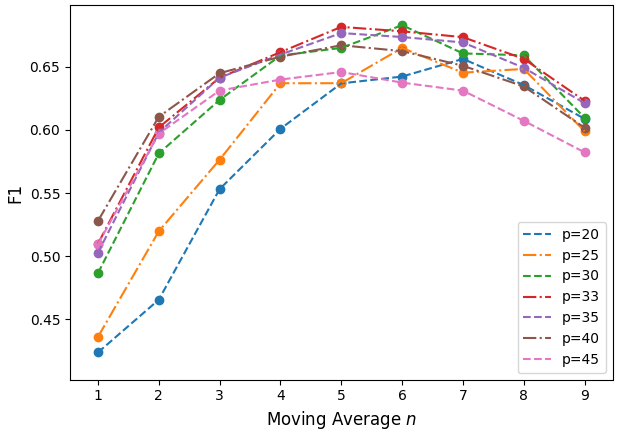
\includegraphics[width=.48\textwidth]{Figures/Fig33.png}}
   \hspace*{\fill}   % maximize separation between the subfigures
   \subfloat[Precision for $p$ and $M$]{\label{fig_2b}
      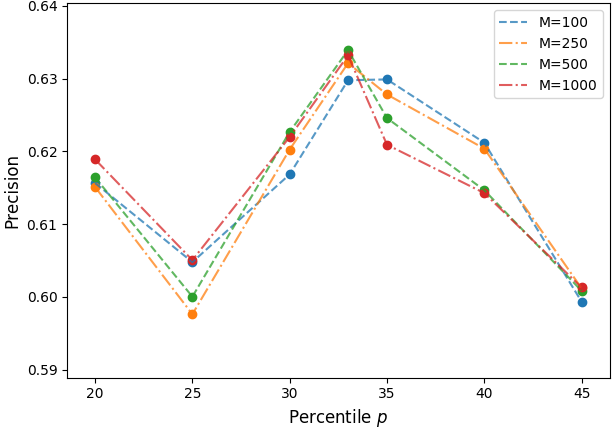
\includegraphics[width=.48\textwidth]{Figures/Fig44.png}}
\\
  \subfloat[Precision for $n$ and $M$]{\label{fig_2c}
      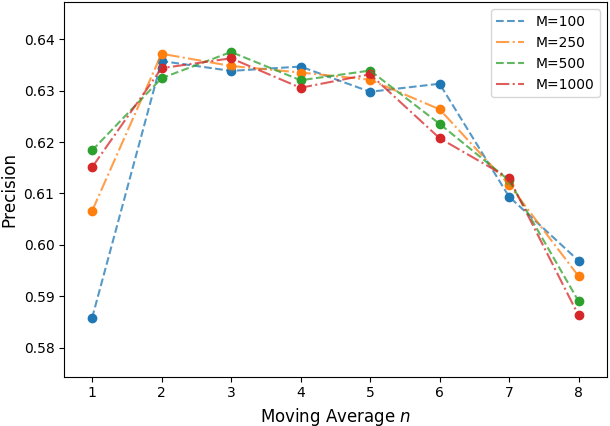
\includegraphics[width=.48\textwidth]{Figures/Fig55.png}}
  \hspace*{\fill}   % maximize separation between the subfigures
  \subfloat[Precision for group size $x$ and $M$]{\label{fig_2d}
      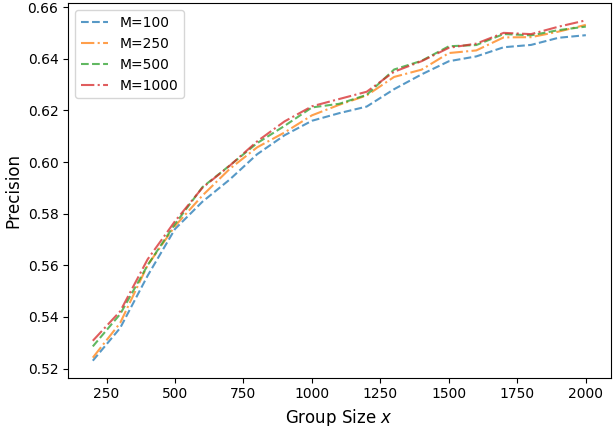
\includegraphics[width=.48\textwidth]{Figures/Replacement.png}}
   \caption[Identifying Best Parameters for Time Distribution]{Variation of ability to predict $UTC^L$ ($t_1=0.5$) with parameter values: (a) F1 vs. moving average window width $n$, for different values of percentile $p$, fixing $M=250$; (b) Precision vs. percentile $p$, for  different sample sizes $M$, fixing $n=5$ which yielded the best F1 score; (c) Precision vs. $n$ for different values of $M$, fixing $p=33$ which yielded the best F1 score; and (d) Precision vs. group size $x$
for different values of $M$, using sampling with replacement, and fixing  $p=33$ and $n=5$.} \label{fig_2}
\end{figure*}

Predictions that were more than $t_1=0.5$ away from $UTC^L$ were marked as incorrect. The following observations emerge from Fig. \ref{fig_2}:

\begin{itemize}
    \item 
Fig. \ref{fig_2}(a) shows F1 for different values of $p$ and $n$ for $M = 250$ and $t_1=0.5$ over all groups in the UTC offset dataset. It can be seen that the best performance with F1 = 68.14\% is achieved using $p=33$ and $n=5$.  
\item
Fig. \ref{fig_2}(b) confirms that $p=33$ is the best performing using precision for four different values of $M$. This value of $p$ is also an intuitive choice because, as mentioned earlier, about a third of the 24-hour period is expected to be devoted to sleep. Smaller percentile ($p<30$) reduces the associated sleeping cycle and it is harder to fit a parabola and to get a good UTC offset prediction. On the other hand, if $p$ is too high ($p\geq40$) then points that are outside of the sleeping cycle will be incorporated causing the performance to suffer. 
\item
%The effect of $n$ is to smooth out the curve, 
Fig. \ref{fig_2}(c) shows that $n \in [2,5]$  exhibit high precision for all values of $M$. From this figure, we conclude that any choice of $n\in [2,5]$ is reasonable to smooth out irregularities, preserve high precision, but is not too high to delete the sleep cycle from the time distribution. However, considering both, the precision and F1,  we conclude that $n=5$ is the best choice. 
\item
When using sample size $M$ the group size needed to be at least $M$ because we have used sampling without replacement. Sampling with replacement allows to better understand whether improvement comes from a bigger sample size or a bigger group size. 
Fig. \ref{fig_2}(d) shows performance for sampling with replacement across different $M$ values as the group size increases (using $n=5$ and $p=33$). We conclude that 
performance is not affected by $M$,  although performance improves with group size.
\end{itemize}

\begin{figure}[!t]
\centering
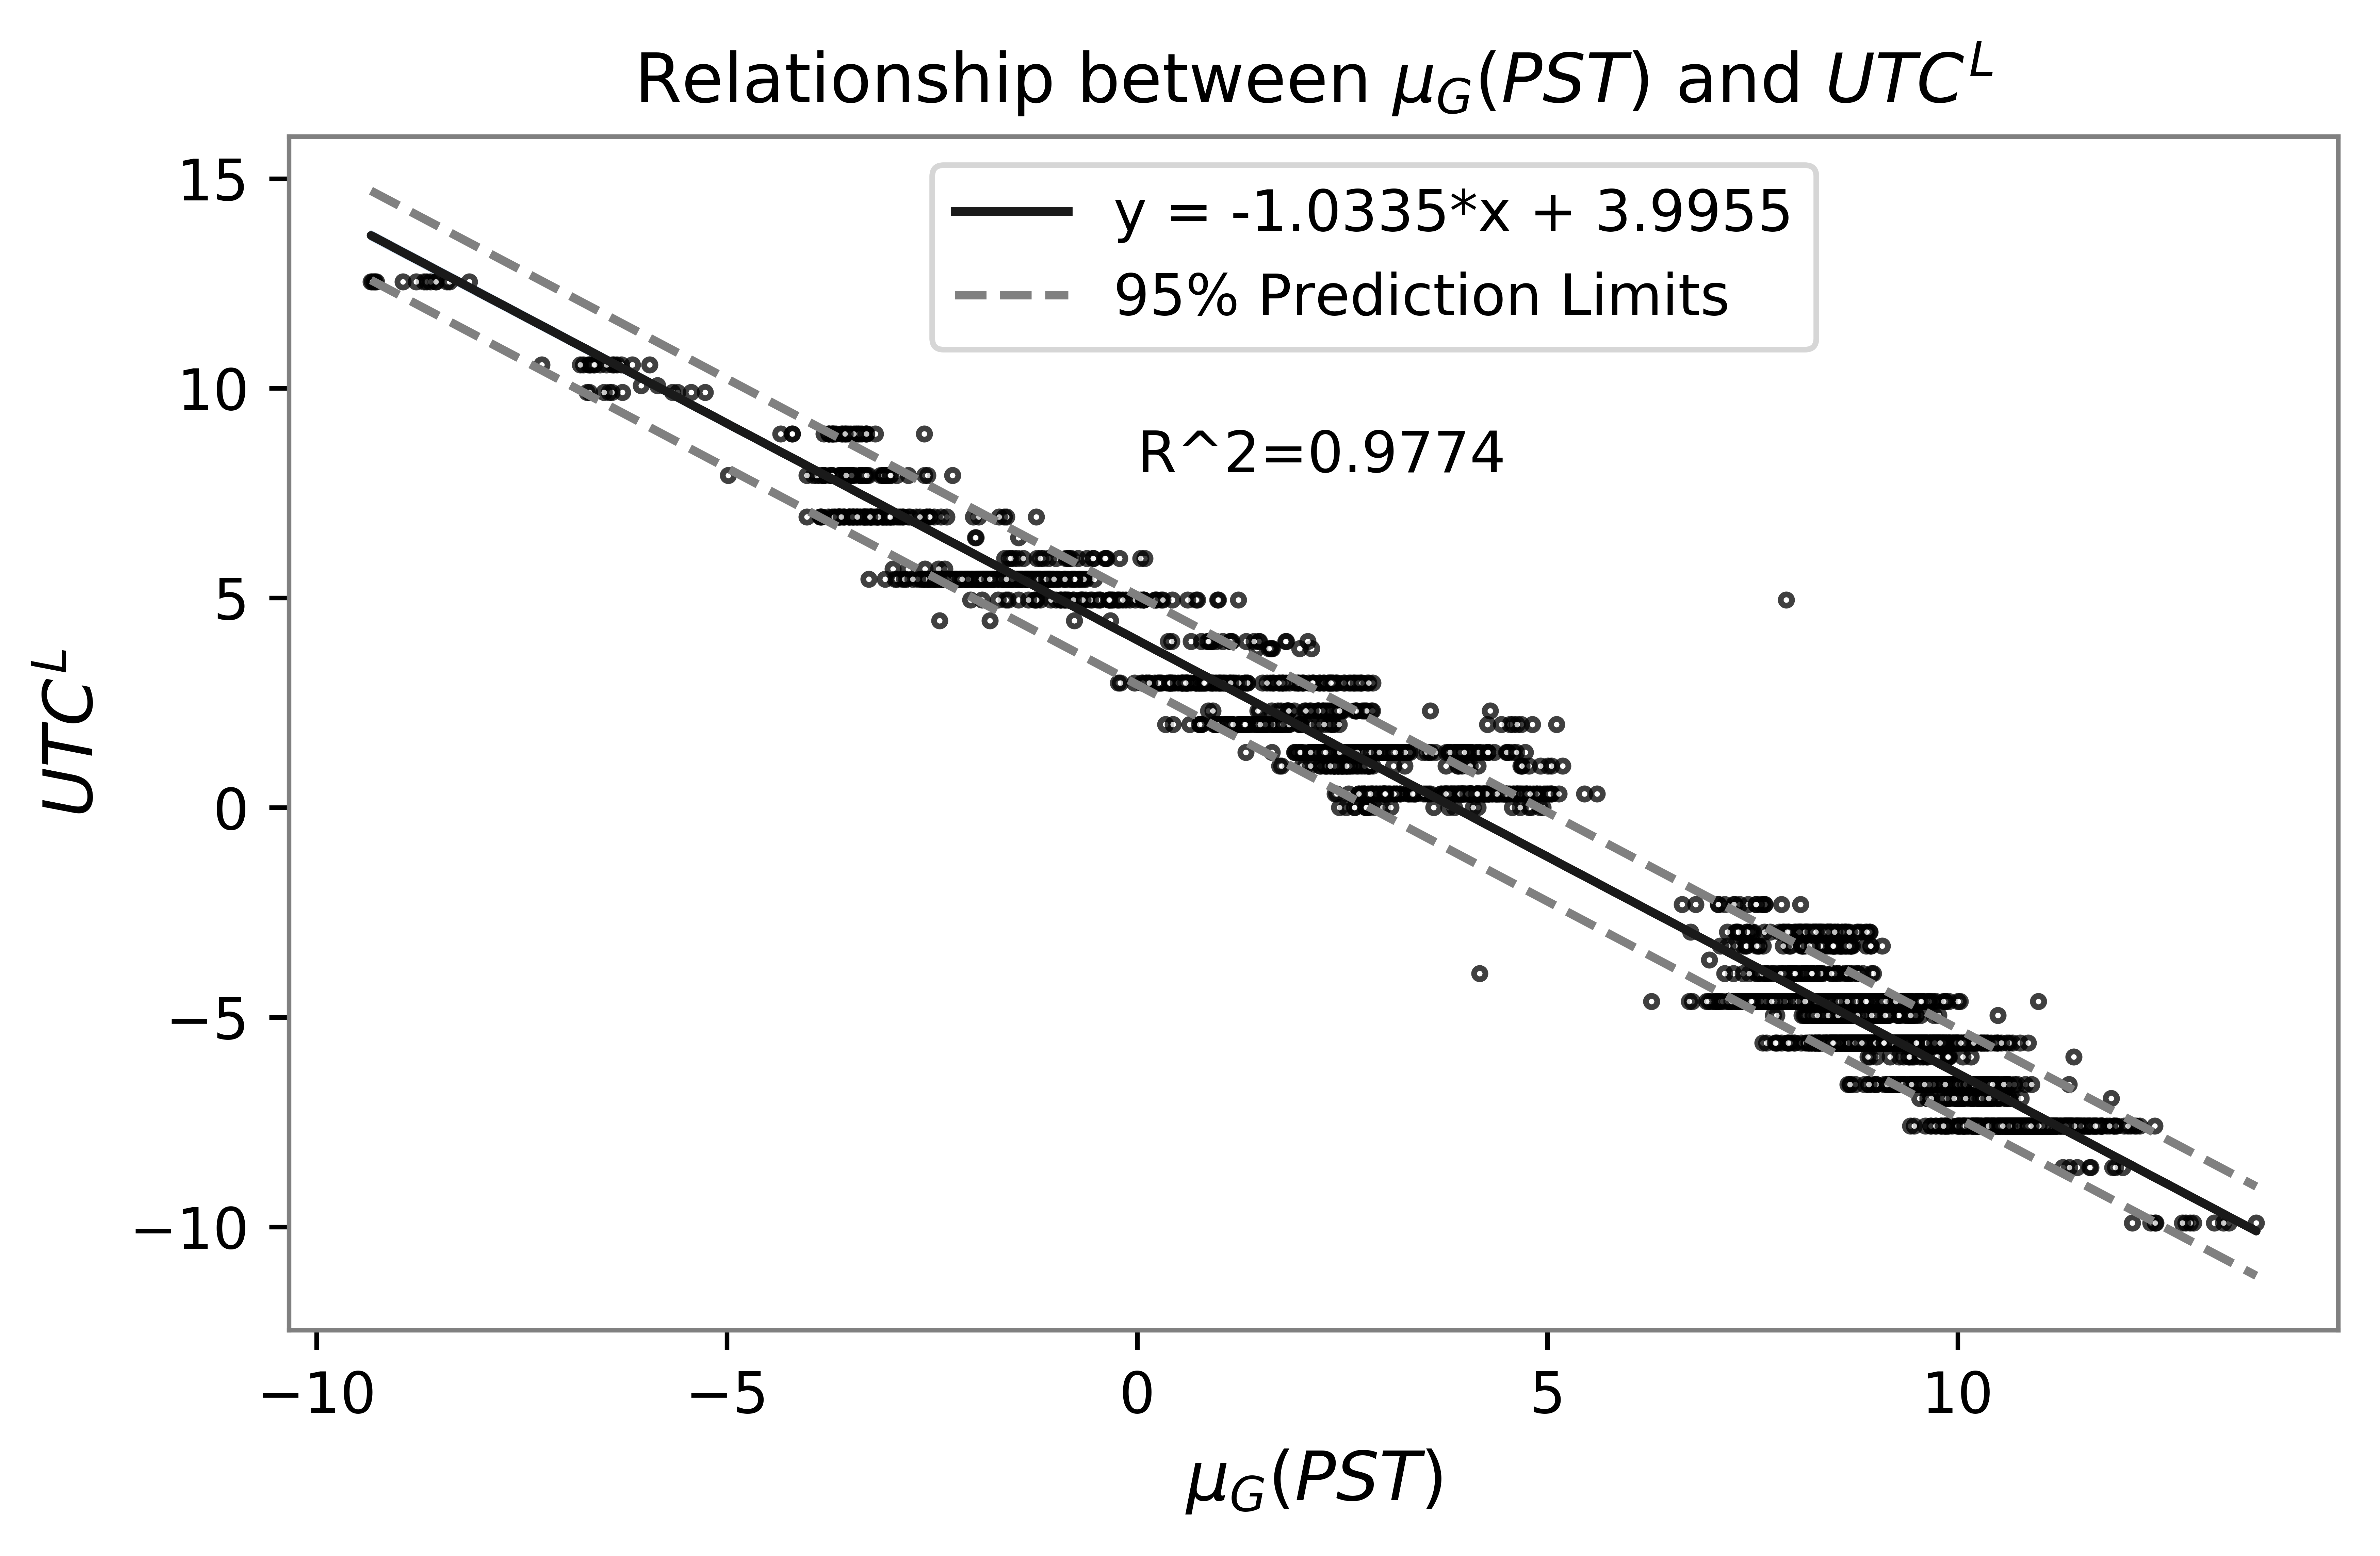
\includegraphics[width=5in]{Figures/filename.png}
\caption[Linear regression between UTC and min of time distribution]{Result of linear regression performed on data points with known geolocation, plotting $UTC^L$ against
$\mu_G({PST})$, with $M=250$, $n=5$, $p=33$, and group size exceeding 1000.}
\label{fig_3}
\end{figure} 

The plot in Fig. \ref{fig_3} uses $M=250$, $n=5$, $p=33$, and group size equal to at least 1000. Using these parameters the relationship between predicted PST %%%%%% WAS UTC, PLEASE CONFIRM ******* (yes should have said PST)
and actual UTC is shown. A linear relationship can clearly be observed, using $UTC^P = -1.0335\times PST + 3.9955$
 with overall $R^2=0.9774$;
 this is approximated as follows:
% equation (\ref{eq001}):

\begin{equation}
UTC^P = -1.0 \times PST + 4.0
\label{eq001}
\end{equation}

\section{Temporal Analysis of Message Traffic data} \label{sec4}
\label{subsec-illustration}

In this section, we illustrate that time-based features can be used for associating persons and topics with a geographic area. The time-based approach is confirmed using message traffic with coordinates.

%The most data on Twitter can be obtained via the streaming API which gives researchers access to an unfiltered stream of tweets. Once message traffic is collected the user that generates the message and the user mentioned in message is used for inferring the social graph. The graph is used for identifying authorities and closely knit communities. Authorities and communities may be related to a certain geographic area, topic, and/or sentiment towards a topic. Messages with coordinates and place mentions or self-reported locations of the users in the graph can be used to filter to those users that are near a specific geographic area. In this section we illustrate that time-based features can be used for high-level geocoding.

Our focus is on understanding the  spatiotemporal aspects of the
 Twitter social graph, 
 connecting senders of messages and users mentioned in the messages. 
We explore the geographical distribution of senders of 
 messages who mention an individual, 
 thereby evaluating the extent to which an influencer (mentioned in the messages) has global influence.
This is often accomplished by analyzing 
 message traffic data, since the full follower-followee
graph cannot be directly collected due to limitations imposed by the free Twitter API.
%Such a social network can be used to extract many useful properties, such as close knit communities and influencers.
%individuals, etc. 
Messages with coordinates and place mentions or self-reported locations of the users can be used to filter out users that are near a specific geographic area; in this manner, influential individuals and communities belonging to a certain geographic area can be identified.  
%Via streaming API Twitter provides unfiltered access   to an  stream of tweets. From the message traffic data a social graph can be generated using the relation between users that generate the message and users that are mentioned in the message. Such a social network can be used to extract many useful properties, such as identify close knit communities, influential individuals, etc. Messages with coordinates and place mentions or self-reported locations of the users can be used to filter out users that are near a specific geographic area and in this manner influential individuals and communities belonging to a certain geographic area, topic, and/or sentiment towards a topic can be identified.  In this section we illustrate that time-based features can be used for high-level geocoding.

\subsection{Message Traffic Dataset}
We collected five days of message traffic data in the first week of December 2020 for a total of 18.67 million messages. This dataset is denoted as $D_{mess}$. Preprocessing consisted of turning each message to lowercase and tokenizing using NLTK library's TweetTokenizer. For each message, the hour was extracted from its creation time. Each token was associated with a set of hours from the set of messages in which the token appears. Tokens that were at least three characters in length and appeared in over 500 messages were retained, resulting in a total of 23,747 tokens.

\begin{table}[htbp]
\small
\caption{Token labels using messages with geolocation tags}
\label{table_M1}
\centering
\begin{tabular}{|c|c|c|c|c|c|}
\hline
\bfseries Token & \bfseries Label & \bfseries NA\_SA & \bfseries AF\_EUR & \bfseries AS\_OC & \bfseries Total\\
\hline
@realdonaldtrump & NA\_SA & 537 & 47 & 19 & 603\\
\hline
@joebiden & NA\_SA & 142 & 14 & 6 & 162\\
\hline
\#oath4ssr & AS\_OC & 18 & 2 & 30 & 50\\
\hline
@narendramodi & AS\_OC & 1 & 0 & 47 & 48\\
\hline
\#gfvip & AF\_EUR & 0 & 35 & 0 & 35\\
\hline
@pmoindia & AS\_OC & 0 & 1 & 33 & 34\\
\hline
@thehill & NA\_SA & 25 & 2 & 0 & 27\\
\hline
@jairbolsonaro & NA\_SA & 27 & 0 & 0 & 27\\
\hline
@nytimes & NA\_SA & 21 & 3 & 3 & 27\\
\hline
@llinwood & NA\_SA & 24 & 1 & 1 & 26\\
\hline
\end{tabular}
\end{table}

\iffalse
\begin{table}[htbp]
\small
\caption{Token labels using messages with geolocation tags}
\label{table_M1}
\centering
\begin{tabular}{|c|c|c|c|c|c|c|}
\hline
\bfseries Token & \bfseries Label & \bfseries NA\_SA & \bfseries AF\_EUR & \bfseries AS\_OC & \bfseries Total & \bfseries Label Ratio\\
\hline
@realdonaldtrump & NA\_SA & 537 & 47 & 19 & 603 & 0.89\\
\hline
@joebiden & NA\_SA & 142 & 14 & 6 & 162 & 0.88\\
\hline
\#oath4ssr & AS\_OC & 18 & 2 & 30 & 50 & 0.6\\
\hline
@narendramodi & AS\_OC & 1 & 0 & 47 & 48 & 0.98\\
\hline
\#gfvip & AF\_EUR & 0 & 35 & 0 & 35 & 1\\
\hline
@pmoindia & AS\_OC & 0 & 1 & 33 & 34 & 0.97\\
\hline
@thehill & NA\_SA & 25 & 2 & 0 & 27 & 0.93\\
\hline
@jairbolsonaro & NA\_SA & 27 & 0 & 0 & 27 & 1\\
\hline
@nytimes & NA\_SA & 21 & 3 & 3 & 27 & 0.78\\
\hline
@llinwood & NA\_SA & 24 & 1 & 1 & 26 & 0.92\\
\hline
\end{tabular}
\end{table}
\fi

Messages that contain location coordinates %then we know where it originated from. 
%This allows us to build the
provide ground truth against which we can evaluate UTC-based predictions. 
Such messages comprised only 0.71\% of all messages in our dataset, consistent with other literature suggesting that the number is less than 1\% [\ref{appendix:1.8}]. 
In our dataset, there were 6,632 messages with point coordinates and 126,765 messages with a place coordinate (bounding box).  


Among 23747 tokens, as many as 20252 were contained in at least one message with coordinates. 
For each token, we record the number of messages that came from the Americas (longitude $\leq$ -25), Europe/Africa (-25 $<$ longitude $\leq$ 65), and Asia/Oceania (longitude $>$ 65). 
For coordinates specified using a bounding box, both the longitude components had to be associated with the same region. A token was assigned a label based on the region which captured the biggest ratio of messages. 
Among the 20252 tokens with coordinate information, we found that 11955 were associated with the Americas, 4991 with
 Europe/Africa, and 3306 with Asia/Oceania. 
 Table \ref{table_M1} shows examples of ground truth generated in this fashion that contain topic or person mentions (NA\_SA = Americas, AF\_EUR = Europe/Africa, and AS\_OC = Asia/Oceania). The number of messages with coordinates are shown for each region and token. The region that captures the most messages is chosen as the label. For example, for @realdonaldtrump the NA\_SA is the label since 537 messages are from it vs. only 47 and 19 for the other regions.

%For each such token its corresponding frequency was calculated. 
%\subsection{Predict Top Trending Tokens by Region using UTC}\label{ms-prediction}
%We went through all the messages where a specific token appears in order to record the hours and use those to generate a time distribution. Those tokens for which a U-shaped parabola could be fitted were recorded along with the associated (i) the predicted UTC offset, (ii) the coefficient $c_2$ and (iii) the coefficient of determination $R^2$.
%The bigger the $R^2$ the more confidence we have in the fitted polynomial. However, a small $c_2$ represents lack of U-shape. 
%\subsection{Identifying Tokens Region}  \label{ms-prediction} Temporal distribution of a specific token can be obtained using the times of associated messages. As in the previous section, we applied the algorithm to identify whether or not U-shaped parabola could be fitted to this distribution and obtained the associated (i) the predicted UTC offset, (ii) the coefficient of the quadratic term, $c_2$ and (iii) the coefficient of determination $R^2$. As before large value of $R^2$ implies more confidence in the fitted polynomial and small $c_2$ represents lack of U-shapeliness. 
\subsection{Predicting Region of Token}  \label{ms-prediction}

We extracted the  hours (from the creation time) associated with all messages in which each token appears. The set of hours  was used to obtain a time distribution and corresponding: (i) predicted UTC offset, (ii) coefficient of the quadratic term, $c_2$, and (iii) coefficient of determination $R^2$ (using the approach in Section 3.2). As before, a large value of $R^2$ implies  greater confidence in the fitted polynomial, and a large $c_2$ indicates  greater localization of influence.

\begin{figure*}[htp]
   \subfloat[Americas]{\label{fig_M1a}
      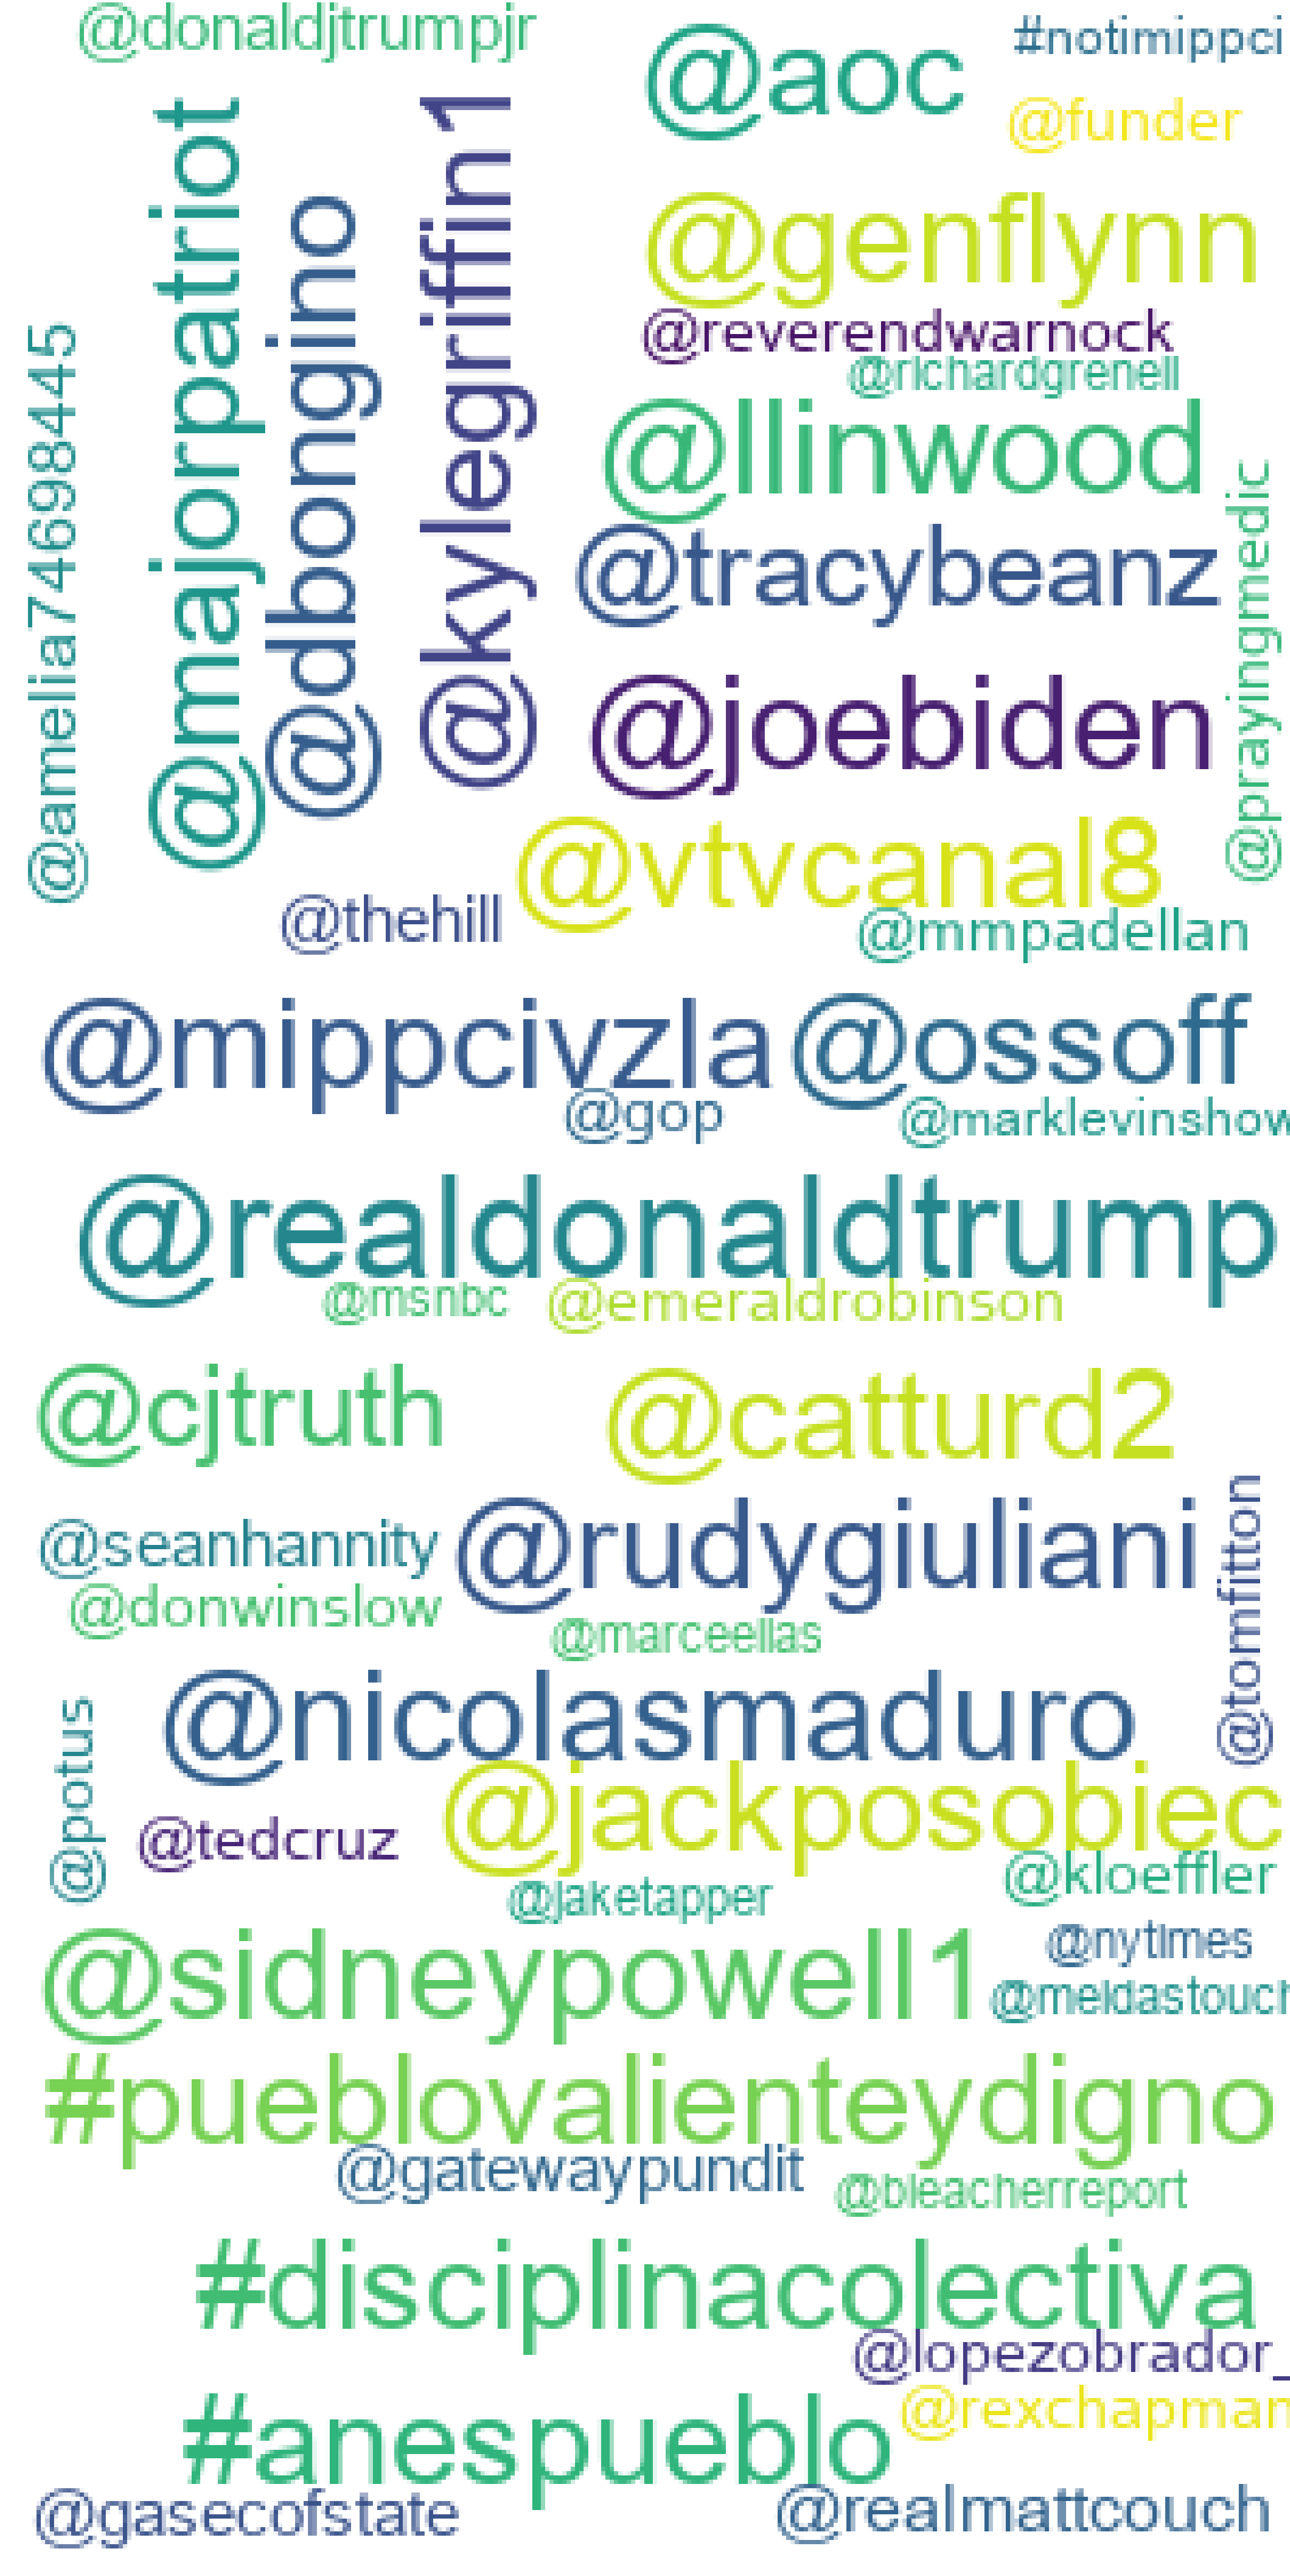
\includegraphics[width=.27\textwidth]{Figures/w1Americas.png}}
   \hspace*{\fill}   % maximize separation between the subfigures
   \subfloat[Europe/Africa]{\label{fig_M1b}
      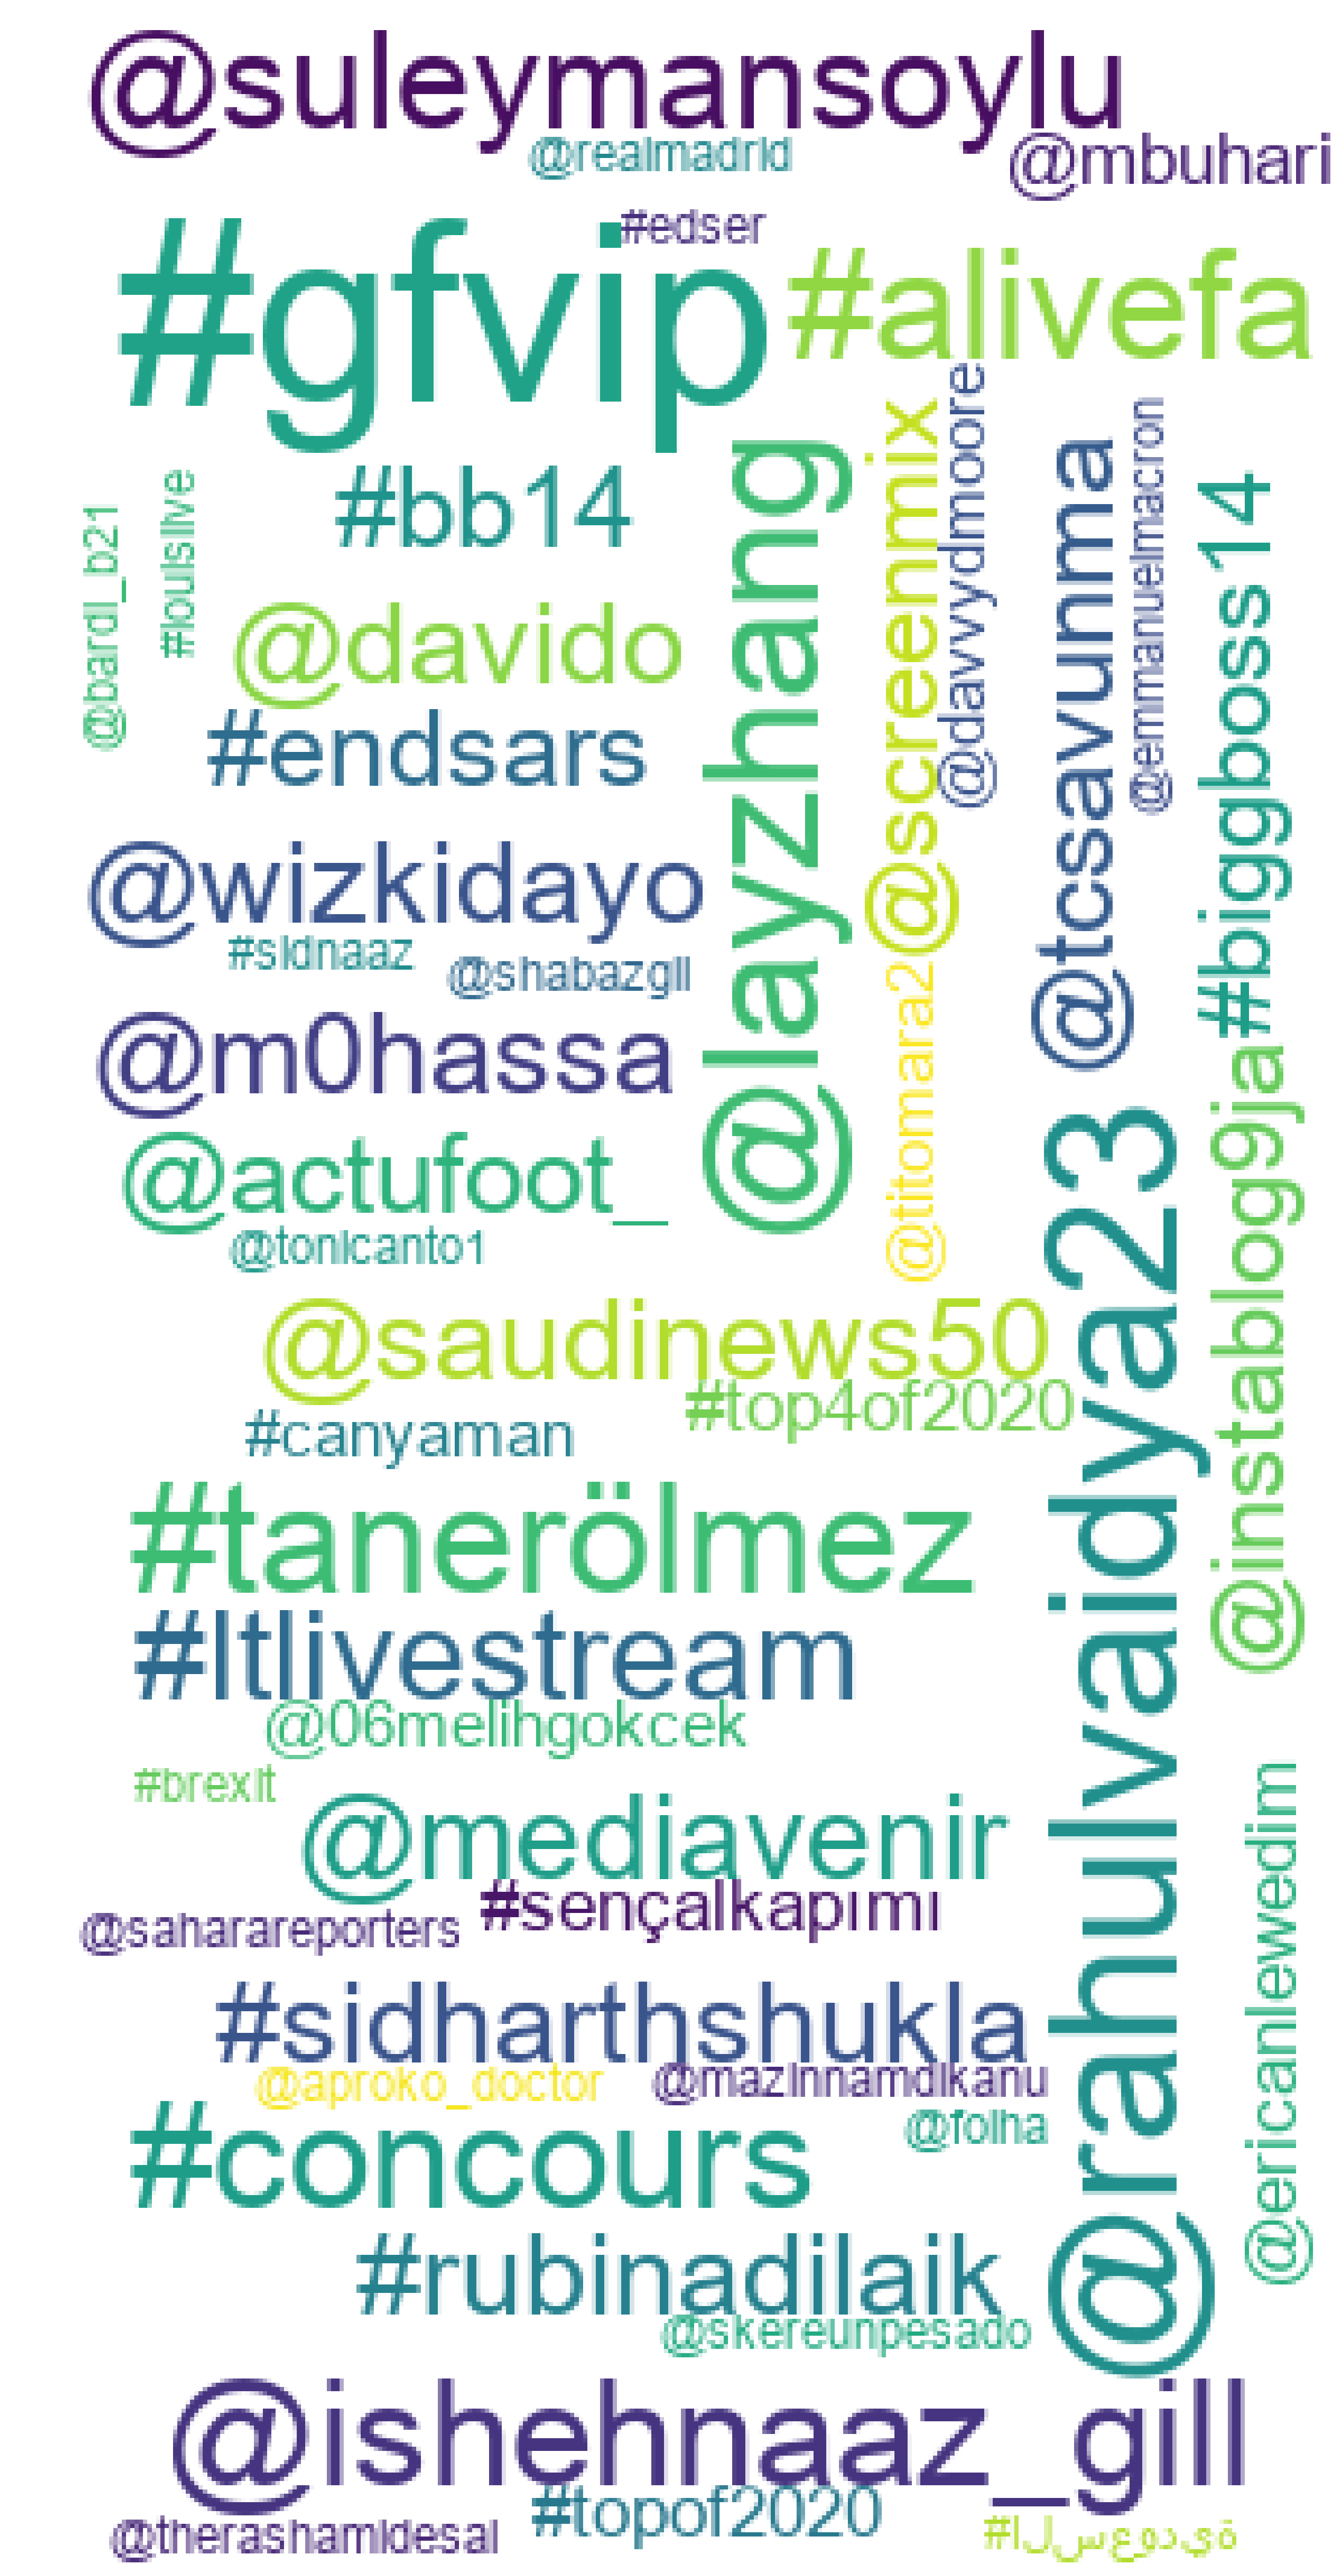
\includegraphics[width=.29\textwidth]{Figures/w3Europe_Africa.png}}
  \hspace*{\fill}   % maximize separation between the subfigures
  \subfloat[Asia/Oceania]{\label{fig_M1c}
      
\includegraphics[width=.29\textwidth]{Figures/Asia_Australia.png}}
   \caption[Predicted Region for Top Trending Keywords]{Top trending tokens (topics and persons) for the (a) North and South America, (b) Europe and Africa, and (c) Asia and Oceania. These were identified using UTC prediction from time curve over message creation times containing the token.} \label{fig_M1}
\end{figure*}

%\subsubsection{Stop Words and U-shape determination}
The NLTK library contains a list of stop-words, such as `the' and `has', which are used worldwide. Their temporal distributions are flat and associated $c_2$ is close to zero.  For example, we found that for stop-words the largest $c_2$ was smaller than $0.001$. To further refine our dataset, we considered $c_2 \geq 0.001$. The result was that not only stop-words but other global topics and persons such as \emph{\#covid19} and \emph{@YouTube} were removed. 

Out of 23747 tokens in the dataset, 16744 contained a sleep cycle that could be used to predict a UTC offset. Based on predicted UTC offset the token was assigned one of three regions: (i) North and South America ($UTC\leq -2$), (ii) Europe and Africa ($-2 < UTC \leq 4$), and (iii) Asia and Oceania ($UTC > 4$). The number of tokens associated with each region was (i) 9618, (ii) 3012, and (iii) 4114 respectively. Of the UTC predictions, 15087 had $R^2\geq0.85$ of which 8487 had $c_2\geq 0.001$. Among these 8487 higher confidence predictions 4135, 1416, and 2936 belonged to each region, respectively. 

As an illustration, Fig. \ref{fig_M1} shows the top fifty words in a word cloud for each geographic region,   focusing on higher confidence tokens that start with $\#$ or $@$ %since these have special meaning on Twitter,
(designating topics or persons).

\subsection{Evaluation}\label{ms-evaluation}
For each token, one of the three regions using UTC prediction is compared with the ground truth, and the accuracy of prediction
%The number of times UTC prediction is accurate 
%(correct vs. total predictions)
is recorded as the ratio of correct versus total predictions, for each region. 

Table \ref{table_M2} shows the results for the three regions. 
The first column shows the type of restrictions placed on a token, % which is 
based on (i) $R^2$ of the polynomial over corresponding sleep cycle, (ii) power coefficient $c_2$ from polynomial, (iii) number of minimum messages, $x$, used to build ground truth, and (iv) whether a collection is limited to persons/topics (@/\#). The accuracy of predictions for each region is shown in columns 3-5 (the respective number of predictions per region is shown in the second column).

%Using UTC predictions tokens are classified to one of the three regions, checked against ground truth region, and number of times UTC prediction is accurate is recorded. Ratio of correct versus total predictions provides the accuracy. Table \ref{table_M2} shows results for the three regions. The first column shows the type of restrictions placed on tokens. The prediction accuracy for each region is shown in columns 3-5 (the respective number of predictions per region is shown under second column). The final column provides overall accuracy. No restriction results show that if a sleep cycle is found and a UTC prediction is made it generally has a good accuracy, but that can be further improved as shown in other rows.

\begin{table}[htbp]
\small
\caption{Performance over Message Traffic}
\label{table_M2}
\centering
\begin{tabular}{|l|l|c|c|c|c|}
\hline
\bfseries Restriction & \bfseries Predictions & \bfseries NA\_SA & \bfseries AF\_EUR & \bfseries AS\_OC\\
\hline
None & 9271, 2825, 2602 & 94.56 & 76.14 & 87.78\\
\hline
$R^2\geq0.85$ & 8611, 2426, 2360 & 95.4 & 80.3 & 89.58\\
\hline
$R^2\geq0.85$, $c_2\geq0.001$ & 4008, 1327, 1976 & 98.6 & 89.9 & 95.29\\
\hline
$R^2\geq0.85$, $c_2\geq0.001$, $x\geq5$ & 3304, 810, 967 & 99.21 & 91.98 & 98.24\\
\hline
$R^2\geq0.85$, $c_2\geq0.001$, $x\geq10$ & 2270, 380, 533 & 99.69 & 94.47 & 98.69\\
\hline
$R^2\geq0.85$, $c_2\geq0.001$, @/\# & 261, 61, 137 & 98.08 & 81.97 & 97.08\\
\hline
\end{tabular}
\end{table}

\iffalse
\begin{table}[htbp]
\small
\caption{Performance over Message Traffic}
\label{table_M2}
\centering
\begin{tabular}{|l|l|c|c|c|c|}
\hline
\bfseries Restriction & \bfseries Predictions & \bfseries NA\_SA & \bfseries AF\_EUR & \bfseries AS\_OC & \bfseries Overall\\
\hline
None & 9271, 2825, 2602 & 94.56 & 76.14 & 87.78 & 89.82\\
\hline
$R^2\geq0.85$ & 8611, 2426, 2360 & 95.4 & 80.3 & 89.58 & 91.64\\
\hline
$R^2\geq0.85$, $c_2\geq0.001$ & 4008, 1327, 1976 & 98.6 & 89.9 & 95.29 & 96.13\\
\hline
$R^2\geq0.85$, $c_2\geq0.001$, $x\geq5$ & 3304, 810, 967 & 99.21 & 91.98 & 98.24 & 97.87\\
\hline
$R^2\geq0.85$, $c_2\geq0.001$, $x\geq10$ & 2270, 380, 533 & 99.69 & 94.47 & 98.69 & 98.9\\
\hline
$R^2\geq0.85$, $c_2\geq0.001$, @/\# & 261, 61, 137 & 98.08 & 81.97 & 97.08 & 95.64\\
\hline
%$R^2\geq0.85$, $c2\geq0.001$, $x\geq5$, @/\# & 128, 24, 50 & 100 & 79.17 & 100 & 97.52\\
%\hline
%$R^2\geq0.85$, $c2\geq0.001$, $x\geq10$, @/\# & 51, 8, 22 & 100 & 87.5 & 100 & 98.77\\
%\hline
\end{tabular}
\end{table}
\fi

Table \ref{table_M2} illustrates that the approach using temporal  distribution is successful. 
The first row, with no restriction, illustrates that if a sleep cycle is found and a UTC prediction is made it generally has good accuracy. The accuracy is  high, particularly for those tokens which have ground truth assembled from more messages (larger $x$) and %which are based of
with high confidence UTC predictions (high $R^2$ and $c_2$). 

About 13\% of the tokens that were labeled using UTC did not have any message traffic with coordinates. A bigger collection could be explored, but there is reason to think that some tokens % %concepts  ??????
just won't get a geo-tag assigned. Fewer than 1\% of messages contained geo-tags, and 38\% of the tokens had fewer than $5$ geo-tagged data points; a prediction based on such a small sample is not made with high confidence. On the other hand, time is available for all messages and each token appeared in at least 500 messages giving us greater confidence in the corresponding time distribution.  This illustrates the usefulness of our approach.

Another alternative would be to utilize the self-reported locations of the users that wrote the messages, but %as already discussed
this would require a complex geocoding solution that can handle the different ways persons refer to locations in various %natural 
languages. Using time distributions  is hence %the best
 a better solution for quickly understanding important keywords in message traffic as they pertain to a geographic region of interest.

\subsection{Comparison against Baseline based on Google Trends}

In a recent paper, Zola et. al. [\ref{appendix:bookChNew5}] attempt to estimate worldwide Twitter user locations without relying on geolocation target labels (no geotagged tweets or user location profiles and no access to geographic dictionaries). Their dataset consisted of 744,830 tweets written by 3,298 users from 54 countries. The location of each user was manually verified. Their approach focuses on nouns (like sites, events, people), which are expected to have a spatial context that is helpful for user location estimation. Each noun was associated with a geographic region based on Google Trends (Google Trends identifies nouns that are trending in various cities). For each user, clustering is used to identify the most probable centroid from coordinates associated with each city. Because no geoinformation is used, the problem is more complex; their approach correctly predicts the ground truth locations of 15\%, 23\%, 39\%, 58\%, 70\%, 82\% of the users for tolerance distances of 250, 500, 1000, 2000, 4000, and 10000 km. Our method also does not utilize any geoinformation, relying only on creation times as the feature, and hence it was appropriate to compare our approach against the one based on Google Trends.

In [\ref{appendix:bookChNew5}] the authors utilize the following approach:
\begin{enumerate}
\item Part of Speech Tagging used to identify a set of nouns for each user.
\item Pytrends Python module is used to associate a noun with a list of cities. Google gives each city a weight, from 0 to 100, based on how popular the noun was (based on how many search queries, originating from that city, contained that noun). Cities with scores of zero are given scores of one so that a non-zero value is present for each city. 
\item Google geocoder Python module (used to get lat, long of each city)
\item Scikit-learn Python library (used to get the centroid) the best method is based on K-means and Density-Based Spatial Clustering of Applications with Noise (DBSCAN) 
\item Centroid is compared to the known location of a user. Median, Mean, and ACC@x (is a user within x kilometers of predicted centroid) are recorded across all users.
\end{enumerate}

We attempt to apply Google Trends to our dataset. In our method we also utilize Pytrends. Pytrend is an unofficial library supporting Google Trends. In function interest\_by\_region() in file pytrends/request.py we change the code so that the Pandas data frame is returned immediately after collecting JSON response from Google. We find that Google, at the `City’ resolution, does return coordinates for each city, it is just that Pytrends did not accurately capture this information. In this way, it is not necessary to geocode each city name with steps (2) and (3) combined (this reduces the potential for introducing errors due to additional geocoding).

There are other differences in that we are focused on all tokens (not just nouns) and we already have three predefined regions that the world is broken up into (so the accuracy will be judged based on how well a region is predicted as was done in previous section). Google Trends ranking is used to predict a region for a token using:
\begin{enumerate}
\item  For each token, we record the set of cities A that came from the Americas (longitude $\leq$ -25), set of cities B that came from Europe/Africa (-25 $<$ longitude $\leq$ 65), and set of cities C that came from Asia/Oceania (longitude $>$ 65).
\item  For each set of cities in A, B, C the cumulative score across the cities in each set are recorded. The cumulative score is based on the ranking returned by Google Trends (Google gives each city a weight based on how popular the token was in the city, weight is from 0 to 100).
\item  A token is assigned to a region that captured the biggest cumulative score.
\end{enumerate}

Because our problem involves large geographic regions it is also appropriate to utilize the `Country’ resolution vs. only `City’. Each country is given the average latitude and longitude of its cities.%\footnote{https://github.com/apanasyu/GoogleTrends}. 

When using Google Trends by region, it can be used to focus on trends that were formed over a predefined time in the past. These are the predefined time ranges: past 1 hour, 4 hours, day, 7 days, 90 days, 12 months, 5 years, all (2004-present) (Google Trends does not allow one to enter a custom date range i.e. it has to be one of these values).  Table \ref{table_5new_1} shows that the trends will result in very different country rankings depending on the time range utilized. The set of country codes in the top three results across the three time frames in Table \ref{table_5new_1} are: KE = Kenya, CA = Canada, US = United States, NO = Norway, IE = Ireland, and CN = China. We choose to focus on 1-year time frame since this is the default option.

\begin{table}
\small
\caption[Top Country Ranking for keyword @realdonaldtrump using Google Trends]{Different time ranges result in very different top 10 country ranking, for keyword @realdonaldtrump, using Google Trends.}
\label{table_5new_1}
\begin{center}
\begin{tabular}{|c|c|c|c|c|}
\hline
\bfseries 1 month & \bfseries 3 month & \bfseries 1 year & \bfseries 5 year & \bfseries all\\
\hline
(KE, 100)&(CA, 100)&(US, 100)&(US, 100)&(US, 100)\\
\hline
(CA, 17)&(NO, 100)&(CA, 84)&(CA, 84)&(CA, 72)\\
\hline
(US, 9)&(IE, 93)&(CN, 35)&(CN, 35)&(IE, 31)\\
\hline
(GB, 4)&(US, 59)&(IE, 34)&(IE, 34	)&(SH, 31)\\
\hline
(AF, 0)&(NL, 54)&(NZ, 30)&(NZ, 30)&(NZ, 29)\\
\hline
(AL, 0)&(DE, 22)&(SH, 30)&(SH, 30)&(PR, 23)\\
\hline
(DZ, 0)&(GB, 21)&(AU, 21)&(AU, 21)&(AU, 21)\\
\hline
(AS, 0)&(PL, 17)&(GB, 17)&(GB, 17)&(KE, 19)\\
\hline
(AD, 0)&(IN, 4)&(NO, 16)&(NO, 16)&(CR, 16)\\
\hline
(AO, 0)&(AF, 0)&(KE, 14)&(KE, 14)&(SG, 16)\\
\hline
\end{tabular}
\end{center}
\end{table}

The number of requests to Google Trends is limited. For example, Python Pytrends library states that 60 seconds of sleep between requests is recommended in avoiding the limit (we have verified that the limit is around 1440 requests, which greatly reduces the amount of data that can be collected daily). In our evaluation, we have focused on 3183 tokens that had $R^2\geq0.85$, $c_2\geq0.001$, $x\geq10$ and 459 tokens that are limited to persons/topics (@/\#) (the results for these presented in the previous subsection in second to last and last row, respectively, of Table \ref{table_M2}).

Table \ref{table_5new_2} and Table \ref{table_5new_3} show the results for the three regions at city and country levels for the 459 tokens and 3183 tokens respectively. The first column shows the type of restrictions placed on Google Trends. Restrictions considered were (i) using only the location with the highest ranking, (ii) using the top three locations, (iii) using locations with a weight $\geq$ 50, and (iv) using all locations. The last row shows the results using our approach based on message creation times. The second column shows the number of predictions made for each region. The precision of predictions for each region is shown in columns 3-5. The final column is the total number of predictions. 

\begin{table}[htbp]
\small
\caption{Performance over 459 Twitter Persons and Topics (@/\#)}
\label{table_5new_2}
\centering
\begin{tabular}{|l|l|c|c|c|c|c|}
\hline
\bfseries Restriction & \bfseries Predictions & \bfseries NA\_SA & \bfseries AF\_EUR & \bfseries AS\_OC & \bfseries Total\\
\hline
City using top 1& 1, 3, 5&100&100&100&9\\
\hline
City using top 3& 1, 3, 5&100&100&100&9\\
\hline
City using weight $\geq$ 50& 1, 3, 5&100&100&100&9\\
\hline
City all	& 1, 3, 5&100&100&100&9\\
\hline
Country using top 1&161, 28, 52&95.03&92.86&100&241\\
\hline
Country using top 3&161, 28, 52&95.65&92.86&100&241\\
\hline
Country using weight $\geq$ 50&161, 28, 52&95.03&92.86&100&241\\
\hline
Country all&161, 28, 52&95.03&92.86&100&241\\
\hline
Our Approach using Time & 261, 61, 137 & 98.08 & 81.97 & 97.08&459\\
\hline
\end{tabular}
\end{table}

Table \ref{table_5new_2} shows that, out of 459 tokens, City Google Trends only produced 9 results while Country Google Trends produced 241 rankings. These tokens contained symbols @ and \# which on Twitter have special meaning, but these are not as common when using the Google search engine. As a result, Google does not have enough information for trend analysis for these tokens. 

\begin{table}[htbp]
\small
\caption{Performance over 3183 popular tokens with at least 10 coordinates}
\label{table_5new_3}
\centering
\begin{tabular}{|l|l|c|c|c|c|c|}
\hline
\bfseries Restriction & \bfseries Predictions & \bfseries NA\_SA & \bfseries AF\_EUR & \bfseries AS\_OC & \bfseries Total\\
\hline
City using top 1&2188, 360, 491&78.29&84.72&83.1&3039\\
\hline
City using top 3&2188, 360, 491&80.94&87.5&84.73&3039\\
\hline
City using weight $\geq$ 50&2188, 360, 491&84.32&90.83&84.11&3039\\
\hline
City all &2188, 360, 491&90.81&94.17&89&3039\\
\hline
Country using top 1&2267, 365, 525&64.49&76.16&88.76&3157\\
\hline	
Country using top 3&2267, 365, 525&55.32&75.07&88.38&3157\\
\hline
Country using weight $\geq$ 50&2267, 365, 525&59.51&78.9&87.62&3157\\
\hline	
Country all&2267, 365, 525&56.64&94.79&80.76&3157\\
\hline
Our Approach using Time & 2270, 380, 533 & 99.69 & 94.47 & 98.69 & 3183\\
\hline
\end{tabular}
\end{table}

Table \ref{table_5new_3} is more informative since the 3183 tokens consist of more common keywords and that tend to be associated with a geographic area. Google Trends has information on most of these with 3039 at the city resolution and 3157 at the country resolution. At the city resolution, it is seen that as more cities are considered the precision is gradually going up i.e. performance using just the top city is the worst. On the contrary, the performance using Country Google Trends has better overall performance when using only the top Country. This could be because there are a lot of separate countries in Europe and Africa continent and as a result, this region tends to be heavily favored when using all countries. When looking at precision across all regions our proposed time-based method performs the best with 98.9\% overall precision vs. the best results via Google Trends at 69.88\% at the country resolution and 90.92\% at the city resolution.

\textbf{Other caveats:}

One might need to adjust Google Trends based on population. For example, when resolution is at the country level the keyword `pizza' is given a weight of 100 for the USA and 99 for Canada. If adjusting for population and number of Twitter users present in the USA vs. Canada, it seems that the USA should be weighted more. Also, the regions are based on the popularity of search areas where Google is used, but Google and Twitter do not have the same popularity around the world. Google trends seem to be case insensitive i.e. `day’ and `DAY’ both return the same results.

Country Google Trends always returns a ranking for 250 countries (with most countries given a weight equal to zero). When the resolution is at the city level Google will return only the top $x$ cities. For the 3183 tokens the average was $x=68.78$ +/- one standard deviation of 26.07 (so statistics are not provided for all cities in the world).

City Google Trends associates tokens with city locations with city names and coordinates available. We recorded all unique city names and coordinates, associated by City Google Trends, over 3183 tokens, into set AllCity (5229 cities recorded). Next, each city name from set AllCity was fed to Google Trends and the top city result and its coordinates were recorded. Distance in miles was computed between the coordinates of a city query vs. the top city via Google Trends. As an illustration, Table \ref{table_5new_4} shows example city tokens and the top city association and the distance between the two.

\begin{table}[htbp]
\small
\caption{Example Google Trends top City vs. Known City Query}
\label{table_5new_4}
\centering
\begin{tabular}{|l|l|c|}
\hline
\bfseries Query City (coordinates) & \bfseries Top Trends City (coordinates) & \bfseries Distance\\
\hline
Barcelona (41.385064, 2.173404)& Barcelona (41.3850639, 2.1734035) & 0\\
\hline
Houston (29.760427, -95.369803)&Bellaire (29.7057858, -95.4588299) & 6.5426\\
\hline
Chicago (41.878114, -87.629798)&Norridge (41.9633641, -87.827284) &11.7575\\
\hline
New York (40.712784, -74.005941)&Albany (42.6525793, -73.7562317) &134.4946\\
\hline
Rochester (41.064765, -86.215833)&Rochester (44.0121221, -92.4801989) &378.8369\\
\hline
\end{tabular}
\end{table}

Across 5229 city queries, 440/5229 = 8.4\%  produced no results. Out of 4789 queries with results, the average distance between city query and city via Google Trends was 362.03 miles +/- 1334.97. ACC@100 was at 87.57\% illustrating that the majority of cities get matched up to a city within 100 miles. However, it is important to highlight that Google Trends is not the same as geocoding i.e. Chicago using geocoder would not get matched up to Norridge, it is just that there were many queries containing Chicago from that location. Similarly, a query such as `Moscow' will not get associated with Moscow Russia because users there will most likely utilize the Cyrillic alphabet. Cities that are popular travel destinations will also be affected.

In summary, Google Trends is an interesting dataset that could be complementary to the time features proposed. The time features were illustrated to perform better for the proposed task, but Google Trends does have interesting properties. The limitations of Google Trends are related to (i) unavailability of data for certain tokens such as popular Twitter topics/persons, (ii) Google Trends is restricted to about 1400 queries per 24-hour period, and (iii) it is not possible to customize the date range over which trends are formed.

\section{Evolving Popularity: Inferring Daily Changes in Number of Followers} \label{sec5}

It is important to understand how an individual's influence changes with time; this can help predict future influence as well. To predict the future one must first understand the past. In the context of Twitter, the corresponding problem involves estimating the rate at which an influencer has gained their existing followers over a given time period. In this section, we propose a novel algorithm to address this problem, using the creation times of an influencer's followers.

To find the number of followers an influencer has gained on a daily basis (i.e., within a span of 24 hours) during a period of $d$ days, one would need $d+1$ daily collections.
Since this is a time-expensive proposition and because Twitter API doesn't allow one to go back in time,   we propose an alternative method for approximating daily gains for  an influencer, and compare it with an approach based on Meeder, et al. [\ref{appendix:5.15}].

\subsection{Dataset: Stable, Global, Growing Influencers}

Each Twitter user's profile contains the number of followers that the user currently has. By collecting user's profile multiple times we can get a sense for how the number of followers is changing. Let $\psi(i, t)$ represent the number of followers of influencer $i$ at time $t$. Let $\psi(i, t_0, t_1)=\psi(i, t_1)-\psi(i, t_0)$ represents the number of new followers $i$ gains during the  time  interval $[t_0, t_1]$; the number of followers stated in influencer's profile at $t_1$ minus the number of followers stated in influencer's profile at $t_0$. 

Twitter keeps track of popular influencers via \emph{@verified}. There are over 300K verified influencers as of this writing. Our focus is on global stable verified influencers that continue to gain followers; to this end, we collected data on influencers that met the following criteria. The influencer:
\begin{enumerate}
    \item having greater than a million existing followers, i.e., $\psi(i,t)>10^6$;
    \item gaining at least a thousand followers within 24 hours,i.e., $\psi(i, t_0, t_1)\geq10^3$ where $t_0$ and $t_1$ are 24 hours apart; 
    \item the gain in the number of followers is less than 1\% of the overall existing follower base, i.e., $\psi(i, t_0, t_1)\leq(0.01 \times \psi(i,t_0))$; 
\end{enumerate}

We ensured that the above criteria were met over three $\psi(i, t_0, t_1)$ collections performed in December 2020. Let $U_0$ contain all verified Twitter influencers. For each influencer $i$ in $U_0$ we computed $\psi(i, t_0=d_0, t_1=d_1)$ where $d_0$ and $d_1$ are 24-hours apart. Influencers that met the three criteria from above form the set $U_1$. For each influencer $i$ in set $U_1$ we ensured that the three criteria were again met using $\psi(i, t_0=d_2, t_1=d_3)$ where $d_2$ and $d_3$ are 24-hours apart to obtain set $U_2$. The process is repeated again using $\psi(i, t_0=d_4, t_1=d_5)$ yielding the final set $U_3$ consisting of 600 influencers.

\subsubsection{Data collected for each Influencer}
The data collected is used to illustrate that $\psi(i, t_0, t_1)$'s,  where $t_0$ and $t_1$ are 24 hours apart,  can be predicted using the creation times. Using an instance of the Twitter API we collected the first 50K followers for each influencer $i \in U_3$.
Twitter API instance is used to record the profile metadata and store them to $allProfile = \{allprofile(t, i): i \in U_3, t \mbox{ refers to the time of collection}\}$. Profile collection is repeated every 5 minutes with the list of collection times given by $PC$.

Another Twitter API instance collects followers. The follower collection, unlike profile metadata, cannot be performed quickly across all influencers. The time when influencer $i$'s followers are collected is recorded as $\mbox{Followers}_t(i)$.

Once the followers for all influencers are collected: given an influencer $i$, $PC$ is used to find a the closest time to $\mbox{Followers}_t(i)$ (which we refer to as $t_1$) and to $\mbox{Followers}_t(i) - \mbox{24 hours}$ (which we refer to as $t_0$). Recall $\psi(i, t_0, t_1)=\psi(i, t_1)-\psi(i, t_0)$, in this case  $\psi(i, t_0, t_1)$=$allProfile(t_1, i)$-$allProfile(t_0, i)$. 

In this way, we have $\psi(i, t_0, t_1)$ over the same period that the followers were collected for all users in $U_3$. In the rest of the chapter, we refer to $\psi(i, t_0, t_1)$ over all users in $U_3$ as the actual 24 hour follower gain, $a_{24}$. 

The followers and the $a_{24}$ over all users in $U_3$ make up our dataset that is denoted as $D_{600}$. Table \ref{table_3N} shows ten influencers from our dataset ordered by the highest $a_{24}$.

\begin{table}[htbp]
\small
\caption{Follower gain for selected influencers over 24 hours}
\label{table_3N}
\centering
\begin{tabular}{|c|c|c|c|c|}
\hline
\bfseries Influencer & \bfseries Follower at t\textsubscript{0} & \bfseries Follower at t\textsubscript{1} & \bfseries a24=Gain\\
\hline
joebiden & 22009684 & 22057780 & 48096\\
\hline
bts\_twt & 31718727 & 31766383 & 47656\\
\hline
bts\_bighit & 26238967 & 26280220 & 41253\\
\hline
arianagrande & 80458070 & 80494729 & 36659\\
\hline
elonmusk & 41178206 & 41208685 & 30479\\
\hline
bighitent & 18527632 & 18553608 & 25976\\
\hline
kamalaharris & 13553348 & 13577323 & 23975\\
\hline
narendramodi & 64532998 & 64556393 & 23395\\
\hline
iamcardib & 15913538 & 15935631 & 22093\\
\hline
nasa & 42743031 & 42763315 & 20284\\
\hline
\end{tabular}
\end{table}

\subsection{An Algorithm to Estimate Follower Gain % over 24 hours
}

%Twitter API can be used to obtain the list of an
%influencer's followers. % are returned by as a list. 
Meeder et al. [\ref{appendix:5.15}] observed that the followers of an influencer are returned by Twitter in a list that is %ordered by recency, beginning with the most recent.
in the order of following time i.e. most recent follower first.
%the most recent follower 
%i.e., given a list [$f_0$, $f_1$, $f_2$] follower $f_0$ is the most recent. 
%Followers $f_0$ and $f_1$ must have followed influencer after $f_2$ had created his/her account.
%%%%%%I'VE MADE CHANGES UPTO HERE SO FAR, 1125PM TUESDAY----CKM******************

Dataset $D_{600}$ for each influencer contains 50K followers. For a specific influencer,  let $\mathcal{L} = [l_0, l_1, l_2, \ldots, l_{49999}]$ be the list of creation times of its followers. We select the first $24 \times n$ values from this list for generating 24 rows of size  $n$ each, denoted as $L_1, L_2, \ldots, L_{24}$. Each $L_i$ is used to generate a time distribution of the creation times. For example, in Fig. \ref{fig_3N}, we have plotted 24 such distributions, using $n = 600$ for the influencer \emph{@CNN}. In this figure, for each distribution, the hour during which the frequency peaks is highlighted in red. We observe that each distribution has a peak and the peak shifts by an hour. Fig. \ref{fig_3N} is drawn for \emph{@CNN} but a similar behavior is observed for most global influencers. In the following, we describe the novel algorithm to estimate an influencer's  daily follower gains. 

\begin{figure}[!ht]
\centering
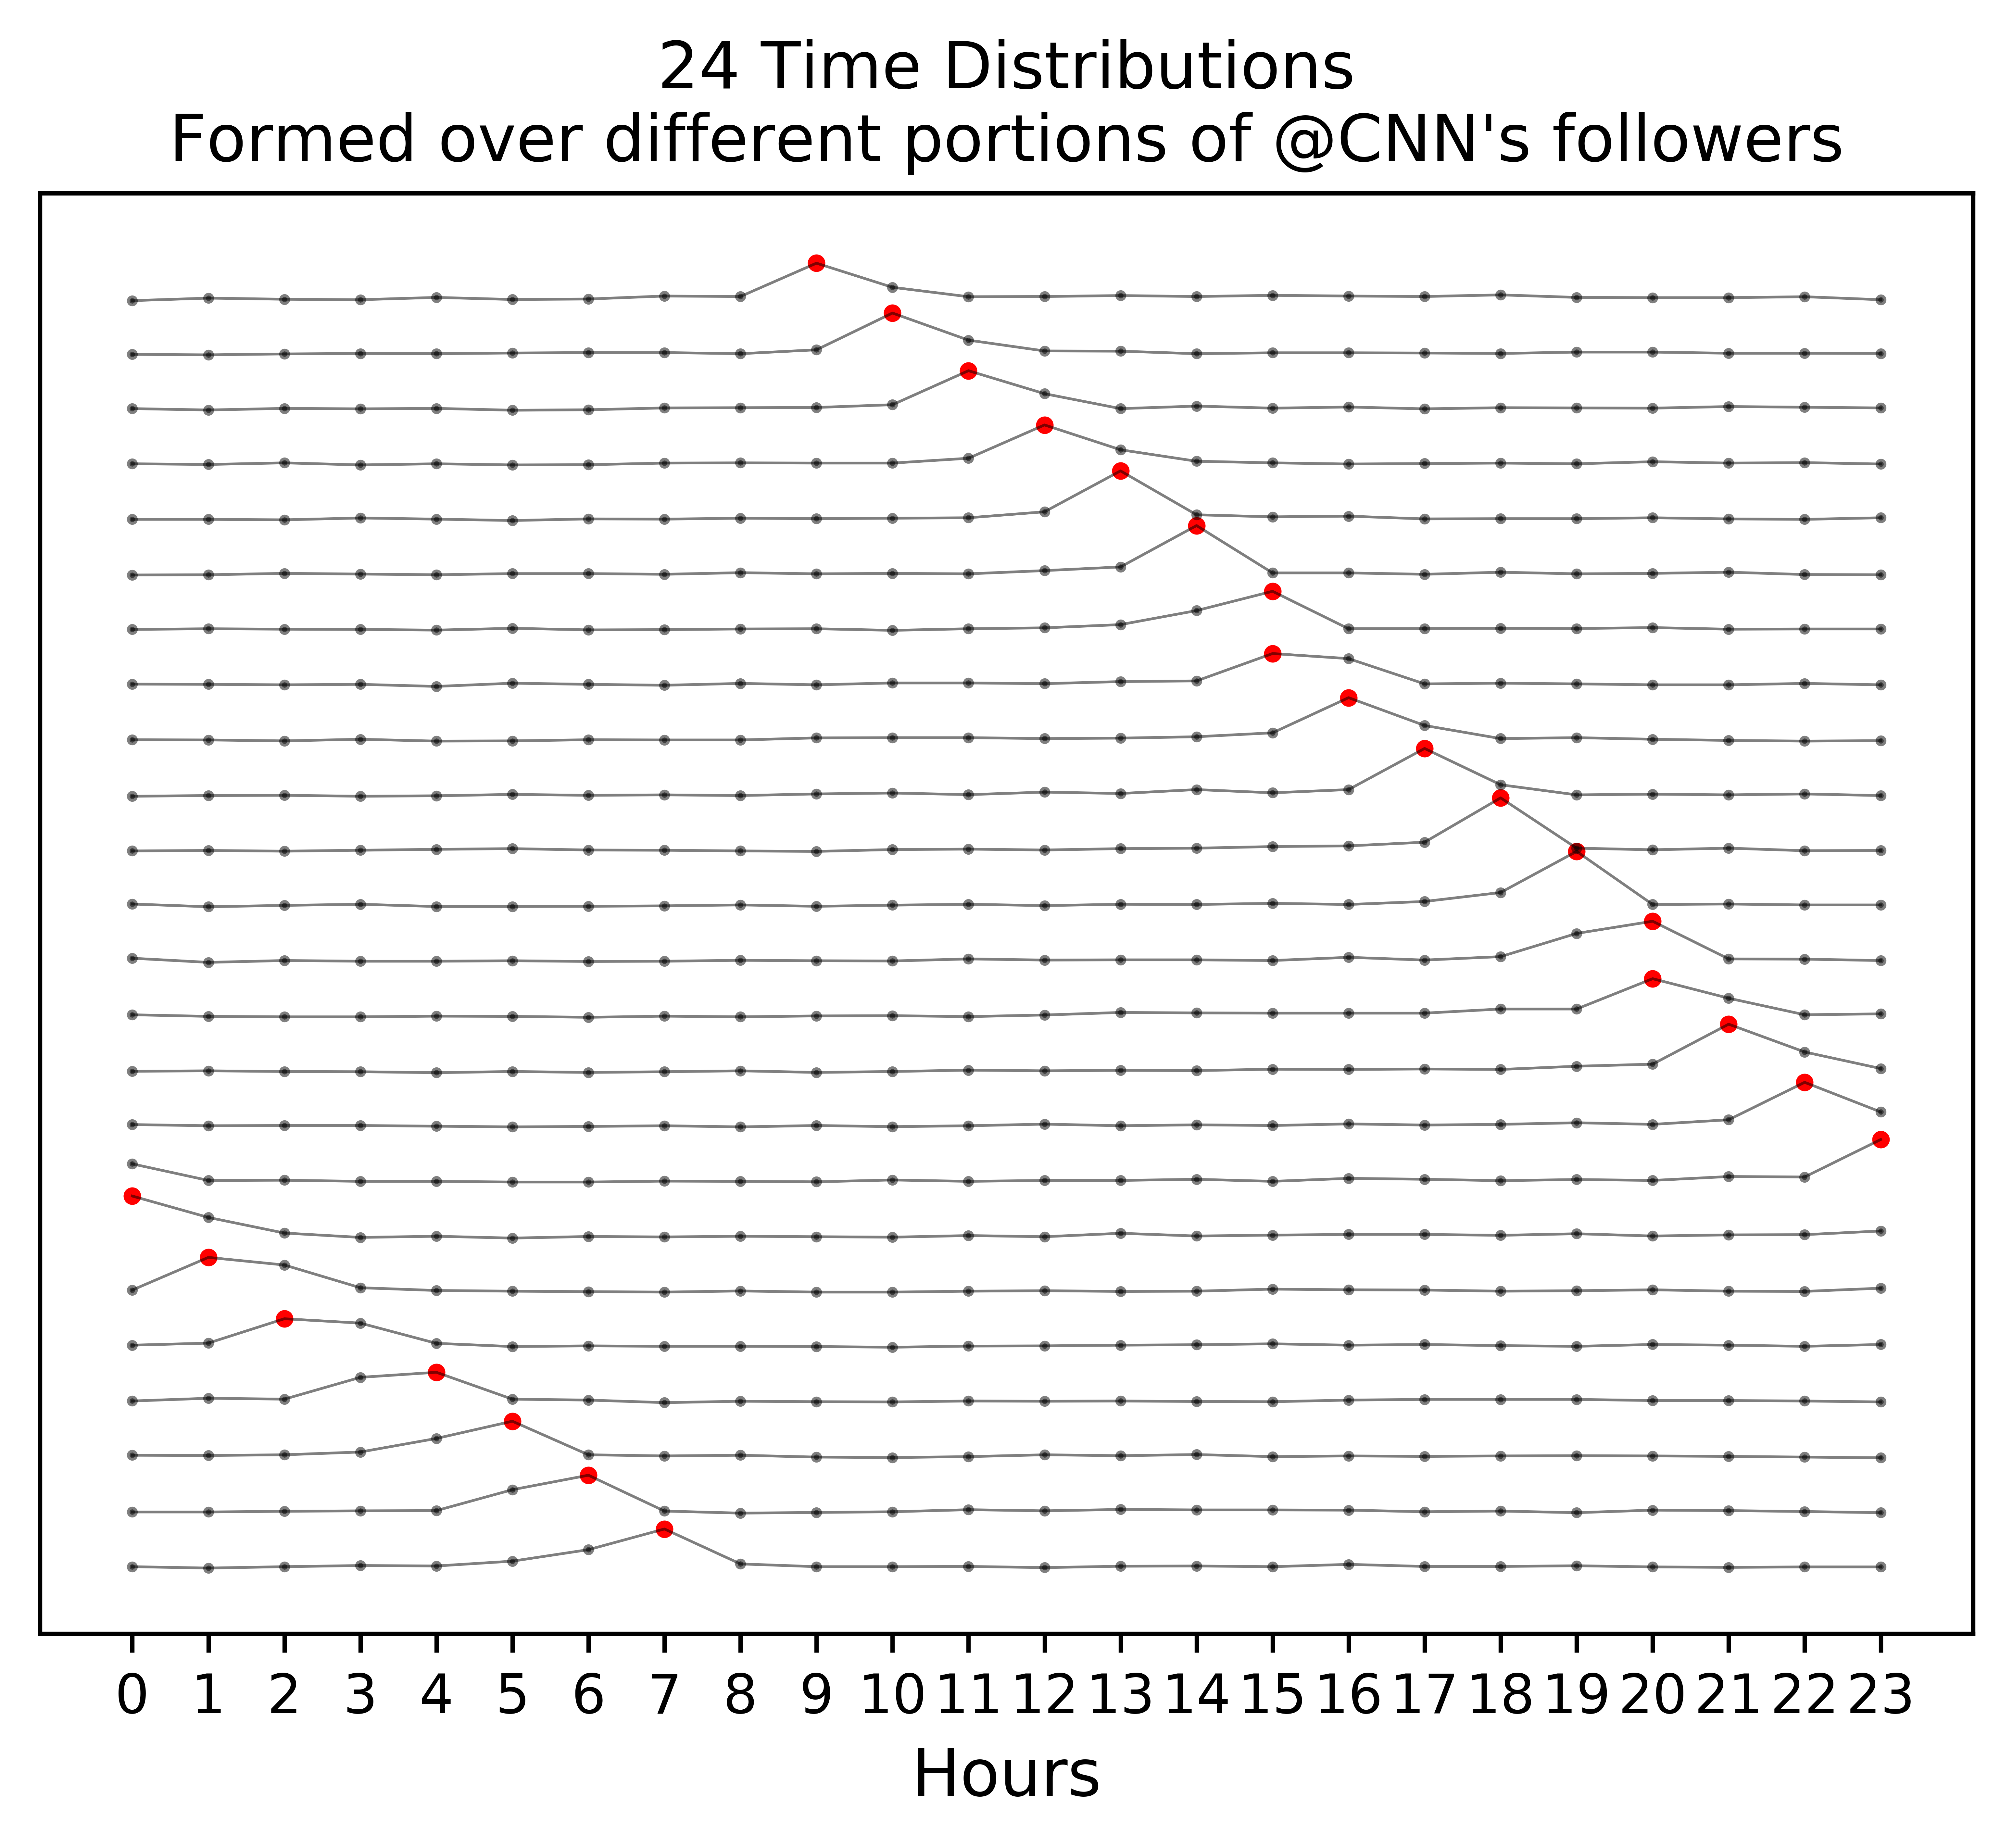
\includegraphics[width=5in]{Figures/Stackedcnn600.png}
\caption[Peak Analysis over Followers of @CNN]{24 time distributions where each time distribution formed from $n = 600$ followers of \emph{@CNN} for a total of $24 \times 600=14400$ followers. Distributions are plotted one above the other ($L_1, L_2, \ldots, L_{24}$). For each distribution the hour during which it peaks is highlighted in red. %Note the cyclical pattern observed by these peaks that in sequence cover all 24 hours.
}
\label{fig_3N}
\end{figure}

\subsubsection{Representing Cyclical Nature of Time}

\begin{figure}[!t]
\centering
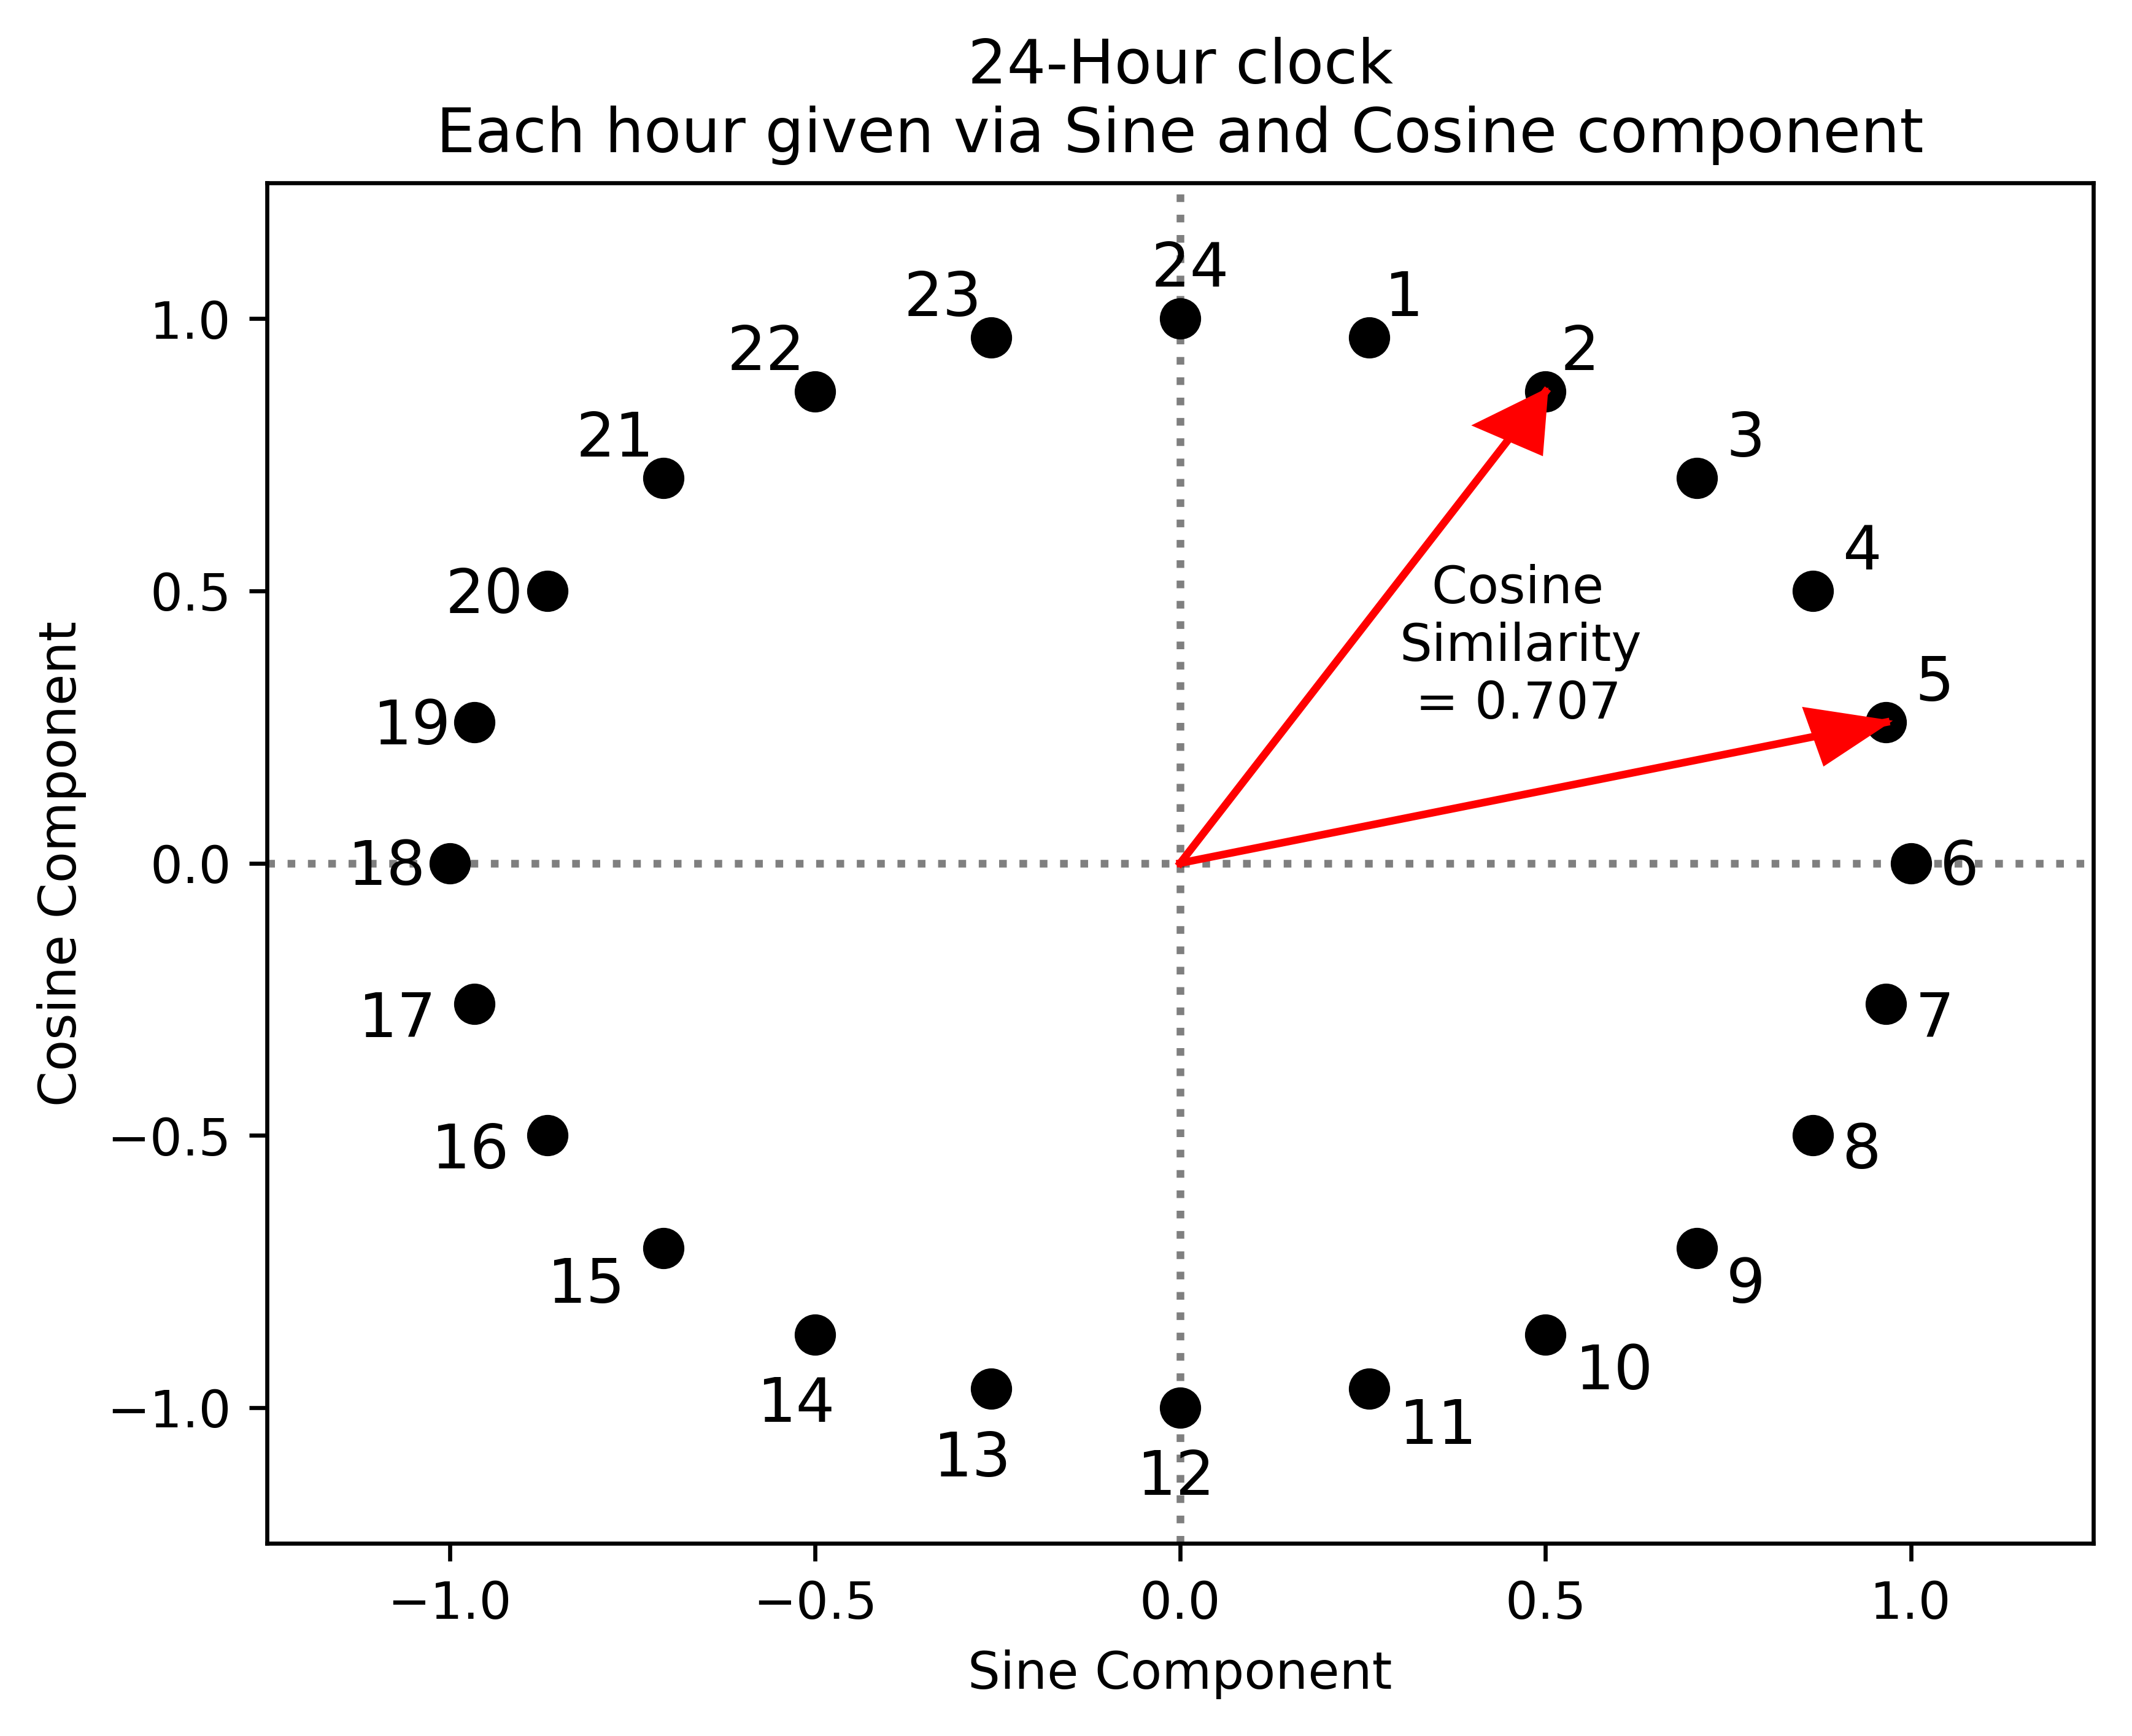
\includegraphics[width=.45\textwidth]{Figures/24HourClock.png}\hfill
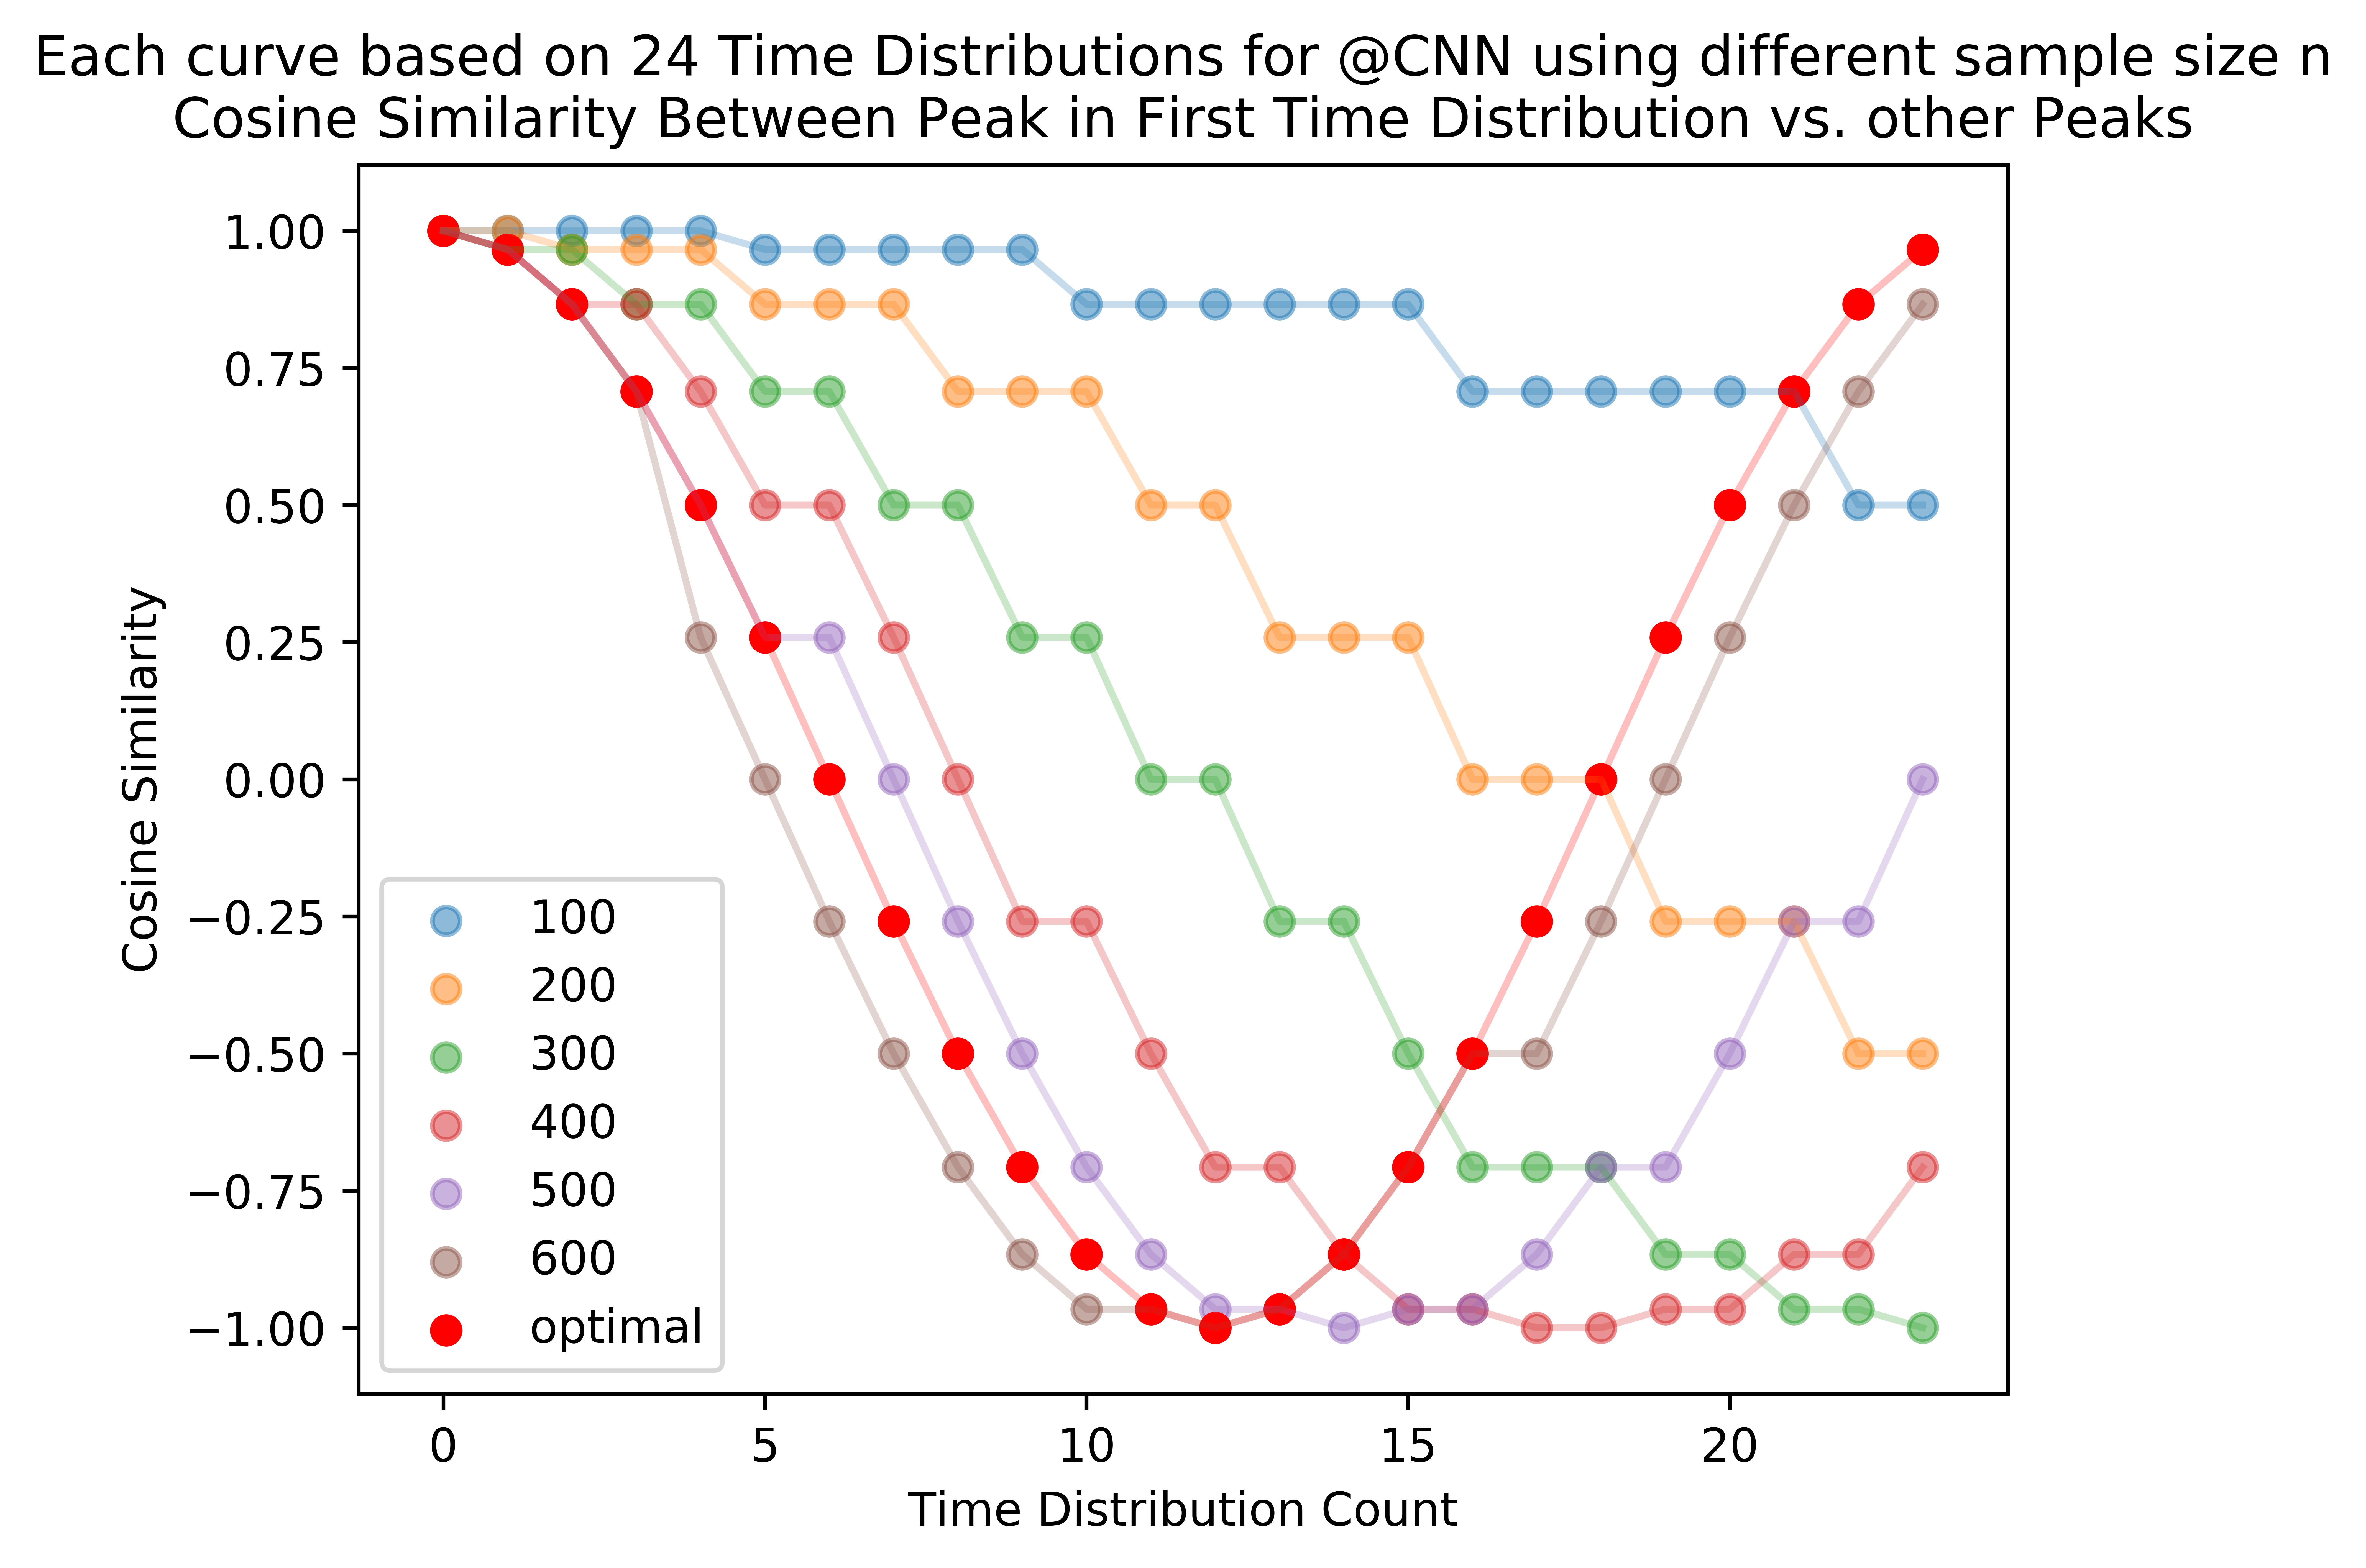
\includegraphics[width=.55\textwidth]{Figures/CosineDistance.png}
\caption[Cosine Similarity using 24-hour Clock]{\textbf{Left} --  24-hour clock; illustrates the computation of the cosine similarity between two hours. \textbf{Right} -- Each curve is computed using cosine similarity between the peak time in the first time distribution vs. itself and peak times over remaining 23 time distributions for various $n$ as described in the text (all graphs for \emph{@CNN}). The red curve is optimal in that the peaks are in the order of the hours on the clock. 
}
\label{fig_5N}
\end{figure}

In the 24-hour clock, shown in Fig. \ref{fig_5N}, each hour can be represented using sine and cosine values of the angle the hour-hand makes with the vertical straight line from the center to the 24\textsuperscript{th} hour. The angle for an hour $h$ in degrees is given as $\textstyle\frac{360 \times h}{24}$. For example,  the angle for 2 O'clock is $\textstyle\frac{360\times2}{24} = 30^o$  and 2 O'clock is represented as $(\sin 30^o, \cos 30^o)$ = (0.5, 0.866). Similarly 5 O'clock is expressed as $(\sin 75^o, \cos 75^o)$ = (0.965, 0.258). The cosine similarity between (0.5, 0.866) and (0.965, 0.258) is 0.707. If we plot the cosine similarities of (sine, cosine) representation of a specific hour A, with  (sine, cosine) representations of hours A, (A+1), (A+2), $\ldots,$ we obtain a smooth cosine curve (see red plot on the right of Fig. \ref{fig_5N}). The vector of the above cosine similarities is denoted as $V_1$ and is called the optimal vector.

Now consider the peak hour in each distribution of \emph{@CNN} in Fig. \ref{fig_3N}. If we compute and plot the vector $V_2$ of cosine similarities between (sine, cosine) representations of these hours with the representation of hour 7 (where the peak occurs in the first distribution), we obtain the brown curve in Fig. \ref{fig_5N}. Likewise, vectors of cosine similarities resulting from sample sizes given by $n$ = 100, 200, 300, 400, and 500 are shown. The similarity between $V_1$ and $V_2$ can be computed using $\rho$, the Pearson Correlation Coefficient. 

We are interested in the size of $n$ that results in temporal distributions that peak exactly one hour apart for all 24 hours (or as close to it as possible). For example, in Fig. \ref{fig_5N}, the curve associated with $n=600$ is closest to the ideal red curve. The key idea is to try different values of $n$ and calculate the associated $V_2$ vectors. The vector $V^*_2$ with the highest correlation against $V_1$ and associated  $n^*$ are obtained. The number of followers gained over 24 hours is predicted as $p_{24} = 24 \times n^*$. A formal description of the algorithm is provided below.
 


\subsubsection{The Algorithm} \label{algo-gain} Input to the algorithm is the list, $\mathcal{L}$, of an influencer's followers  and the precomputed optimal vector $V_1$.  Next,  $n$ is chosen from a minimum of 10 to a maximum of $\lfloor\frac{|L_1|}{24}\rfloor$. For each $n$, 24 time distributions are generated and from each, the hour during which the time distribution peaks is recorded. $V_2$ is generated using cosine similarity between the %first peak hour vs. the sequence of other peak hours.
peak hour in first time distribution vs. peaks across all 24 time distributions.
$V_1$ and $V_2$ are compared using the Pearson Correlation Coefficient $\rho$. The sample size $n^*$ that resulted in the highest correlation coefficient is returned. The predicted 24 hour followers turn over, $p_{24}$, is given as $ 24 \times n^*$.

{\fontfamily{pcr}\selectfont
\begin{tabbing}
\textbf{Al}\=\textbf{go}\=\textbf{ri}\=\textbf{th}\=\textbf{m 1}\=: \textit{infer24HF(L1)}:\\
\> \textbf{Input}: List L1 of follower creation times; \\
\> \textbf{Output}: Predicted 24 Hour Follower Gain, associated\\
\> Pearson Correlation, and number of unique peaks;\\
\> bestN, maxP, maxH = 0, 0, 0;\\
\> V1 = vector of cosine similarities between\\
\> \> \> hour 0 and hours [0, 1, 2, ..., 23];\\
\> for n in [10, 15, ..., |L1|/24]:\\ 
\> \> Split first 24*n elements of L1 into 24 bins of size n;\\
\> \> Record the hour with most elements for each of 24 bins;\\ 
\> \> V2 = vector of cosine similarities between\\
\> \> \> \> hour in bin 1 and hours in each bin;\\
\> \> P = Pearson Correlation between V1 and V2;\\
\> \> if P $>$ maxP:\\
\> \> \> bestN = n;\\
\> \> \> maxP = P;\\
\> \> \> maxH = number of unique peaks across bins;\\
\> Return bestN*24, maxP, maxH; \\ 
end 
\end{tabbing}
}

\subsection{Evaluation}

For each influencer in $D_{600}$, we compute $p_{24}$ and compare it to known follower gain $a_{24}$, using the comparison measure \textit{diff($p_{24}$, $a_{24}$)} = max($p_{24}/a_{24}, a_{24}/p_{24}$)-1.

Fig. \ref{fig_6N} shows the scatter plot of $p_{24}$ versus $a_{24}$ for all influencers in $D_{600}$. The scatter plot is color-coded: green dots represent  influencers with \textit{diff}$\le 0.25$, and red dots represent large differences with \textit{diff}$>1.0$. The Pearson correlation coefficient between  $p_{24}$  and $a_{24}$ vectors is $\rho =0.967$, a high value that shows that the proposed  method makes  accurate predictions. %For example, for  \emph{@CNN} $n^* = 625$ and the  predicted gain is  $ (n*24 = 15000)$;  whereas the actual gain  is 15617.

\begin{figure}[!t]
\centering
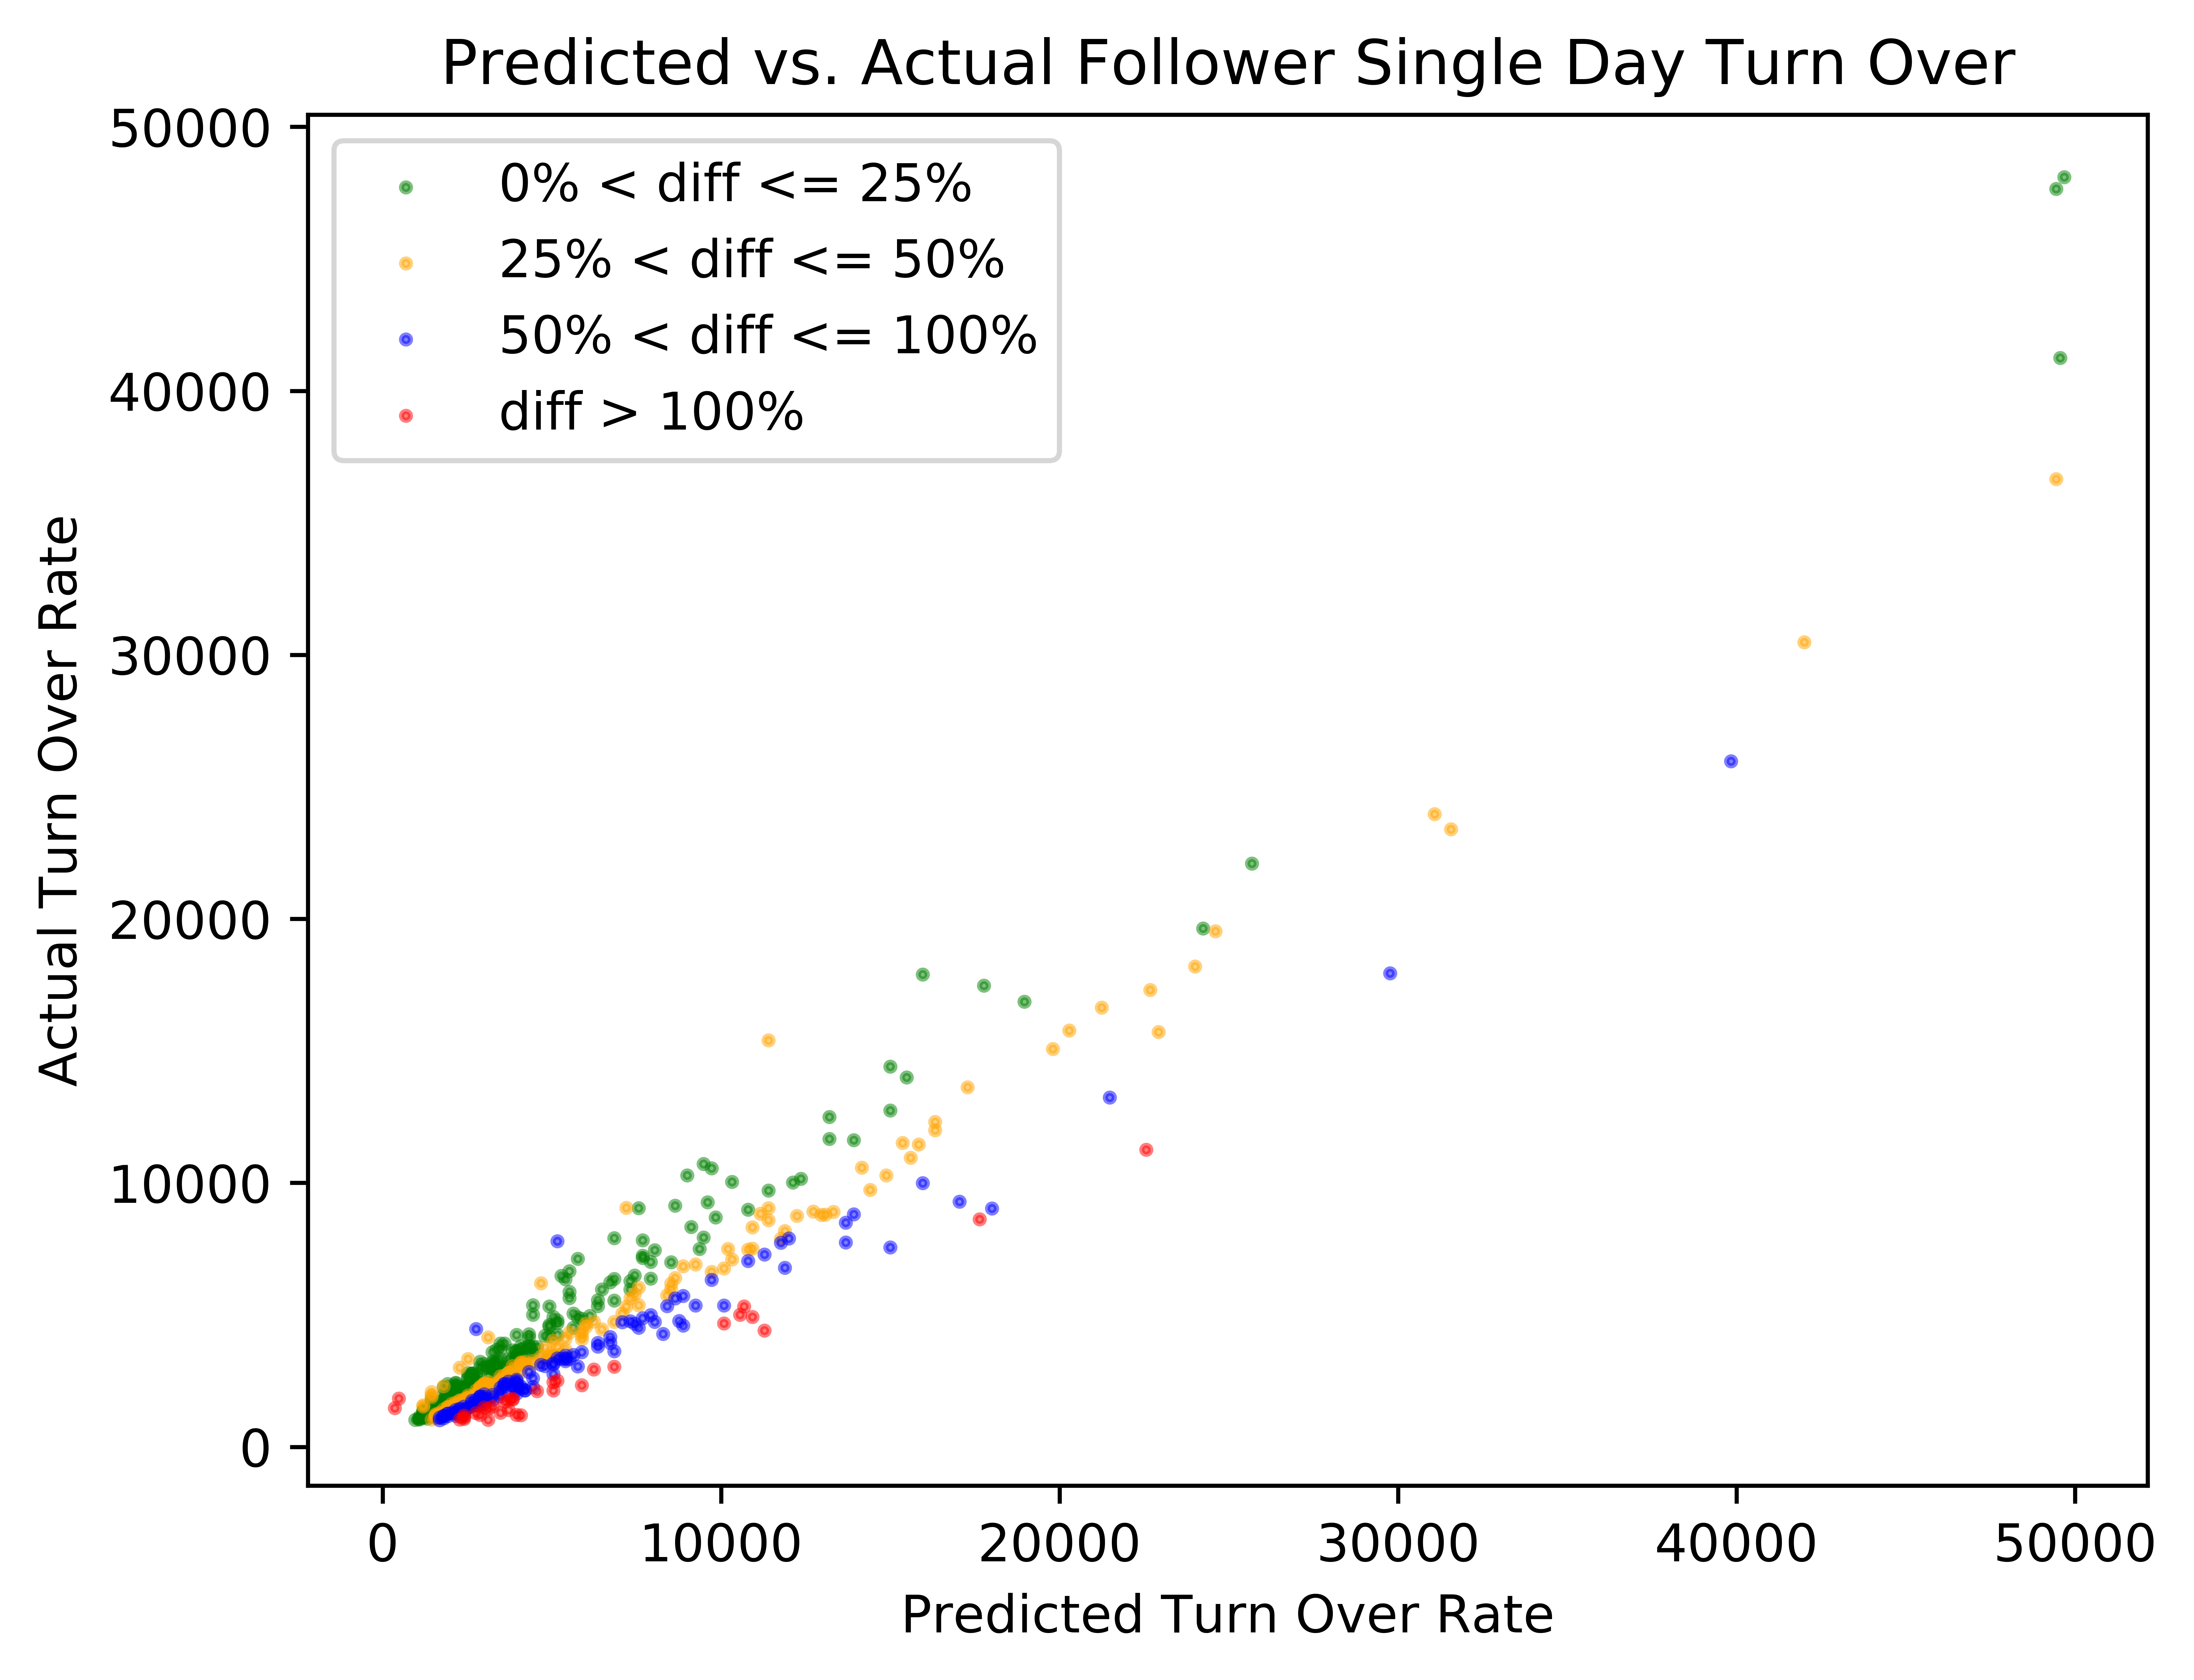
\includegraphics[width=4.5in]{Figures/percturnRate.png}
 \caption[Scatter plot of Inferred vs. Actual daily follower gain]{Scatter plot of Inferred vs. Actual number of followers gained by 600 influencers over a 24-hour time period (Pearson correlation coefficient = 0.967);  238 points (green) differ by  $<25$\%, 195 points (orange) differ by $<50$\%, 126 points (blue) differ by  $<100$\%, and 41 points (red) differ by $\geq100\%$.}
\label{fig_6N}
\end{figure}

We compare our algorithm against two baselines. Meeder et al. [\ref{appendix:5.15}] provide a method for estimating when a user had followed the influencer. Given a list of followers' creation times $L_1$ for influencer $i$, the follow time for a follower at index $j$ is approximated by max($L_1[j:]$) (max gives the most recent creation time at indices greater than or equal to $j$). For our problem we are interested in the number of followers gained over 24 hours so that the datetime max($L_1[j:]$) is as close to the datetime that is 24 hours before the follower collection took place (given by $\mbox{Followers}_t(i)$ minus 24 hours). Effectively we are trying to utilize the method proposed by Meeder to estimate the index $j$ that would satisfy this requirement. The method should work for those influencers that are likely to be followed by brand new users immediately after their account creation. 

%We implemented two baselines based on the method proposed by Meeder et al. [\ref{appendix:5.15}]. 
$\mbox{Followers}_t(i)$ gives time $t$ for influencer $i$'s followers collection.  %Let $\mathcal{L}_M$ be the list such that 
Let $\mathcal{L}_M[j] =$
$(t-\mbox{ creation time of the }   j^{th}  \mbox{ follower of the influencer}$, for $j = 0, 1,  \ldots)$. 
%The first prediction of the influencer's follower gain is obtained as follows:

\subsubsection{Baseline 1:} Traverse the list, $\mathcal{L}_M$, in reverse order and find the first index $j$, such that $\mathcal{L}_M[j] \leq \mbox{ 24 hours}$. If such a $j$ exists, then return $j+1$, denoted as $p_{24}^{(B1)}$; else return $|\mathcal{L}_M|$. 

\subsubsection{Baseline 2:} For each $j$, such that $\mathcal{L}_M[j] \geq \mbox{ 24 hours}$ calculate $\frac{\mathcal{L}_M[j]}{j+1}$; Find the minimum ratio, which will approximate the average number of seconds that elapse per new follower; Return $p_{24}^{(B2)} =$ $\frac{86400}{ratio}$ (since there are 86400  seconds in 24 hours).

As before, we can calculate the correlation coefficient between the vectors of $p_{24}^{(B1)}$ and $a_{24}$ and between $p_{24}^{(B2)}$ and $a_{24}$ over all influencers. In addition, median error and MSE can be computed, where diff(predictions, $a_{24}$) is the error that is to be minimized. Table \ref{table_24HEval} shows how our approach  compares against baseline predictions based on these measures. 
%It can be seen that a
Correlation values of all three approaches are high, with slightly better values obtained by our approach.
In terms of median error and MSE,
 our approach performs much better than the baselines.
%perform well , but our method performs slightly better in all three measures. 
%Given this performance we also recommend utilizing the second baseline as an additional check against our method. 
\begin{table}[htbp]
\small
\caption{Performance of three algorithms to predict influencers' gains}
\label{table_24HEval}
\centering
\begin{tabular}{|c|c|c|c|}
\hline
\bfseries Approach & \bfseries Correlation & \bfseries Median Error & \bfseries MSE\\
\hline
Baseline 1 ($p_{24}^{(B1)}$)  & 0.962 & 0.620 & 0.665\\
\hline
Baseline 2 ($p_{24}^{(B2)}$)   & 0.964 & 0.541 & 0.510\\
\hline
Our  & 0.967 & 0.298 & 0.252\\
\hline
\end{tabular}
\end{table}

%\subsection{Rationale for improved performance} %Why the Algorithm works
\subsection{Rationale for Proposed Algorithm and its Limitations} %Why the Algorithm works
If we consider a group of users that %have performed an action
acted during a specific hour $h$ (such as posting a message or following another), then we are likely to observe a maximum near that same hour in their creation time distribution. This behavior has been confirmed, as discussed below, by analyzing time distribution for users grouped using the time that they have posted a message.

We utilize the dataset  $D_{mess}$. We take all messages that contain a specific token. For example, for token `@youtube' there were 13704 messages. Next, we separate the messages (containing that token) by the hour of message creation time. In this way, 24 groups of users are formed where each user group is known to have been active during a specific hour (the hour during which the message was generated). For each user group, we construct the creation time distribution. 

Fig. \ref{fig_Explanation}(a) shows a heat map for the 24 time distributions generated for token `@youtube'. Notice that a global concept `@youtube' will have a pattern down the diagonal like an Identity Matrix (`@youtube' considered global because $c_2<0.001$); the same analysis was performed using stopwords such as `the' and `you' and they also observe this pattern. The pattern is due to a unimodal distribution that peaks near the same hour as the hour during which the users were most active in generating the messages. Intuitively if a person had the time for creating their Twitter account in the morning then this person is likely to be active on the Twitter platform during the same morning hours in the future (there is thus a correlation between the creation times and activity times).

\begin{figure*}[htp]
   \subfloat[Messages with `@youtube']{\label{fig_Explanationa}
      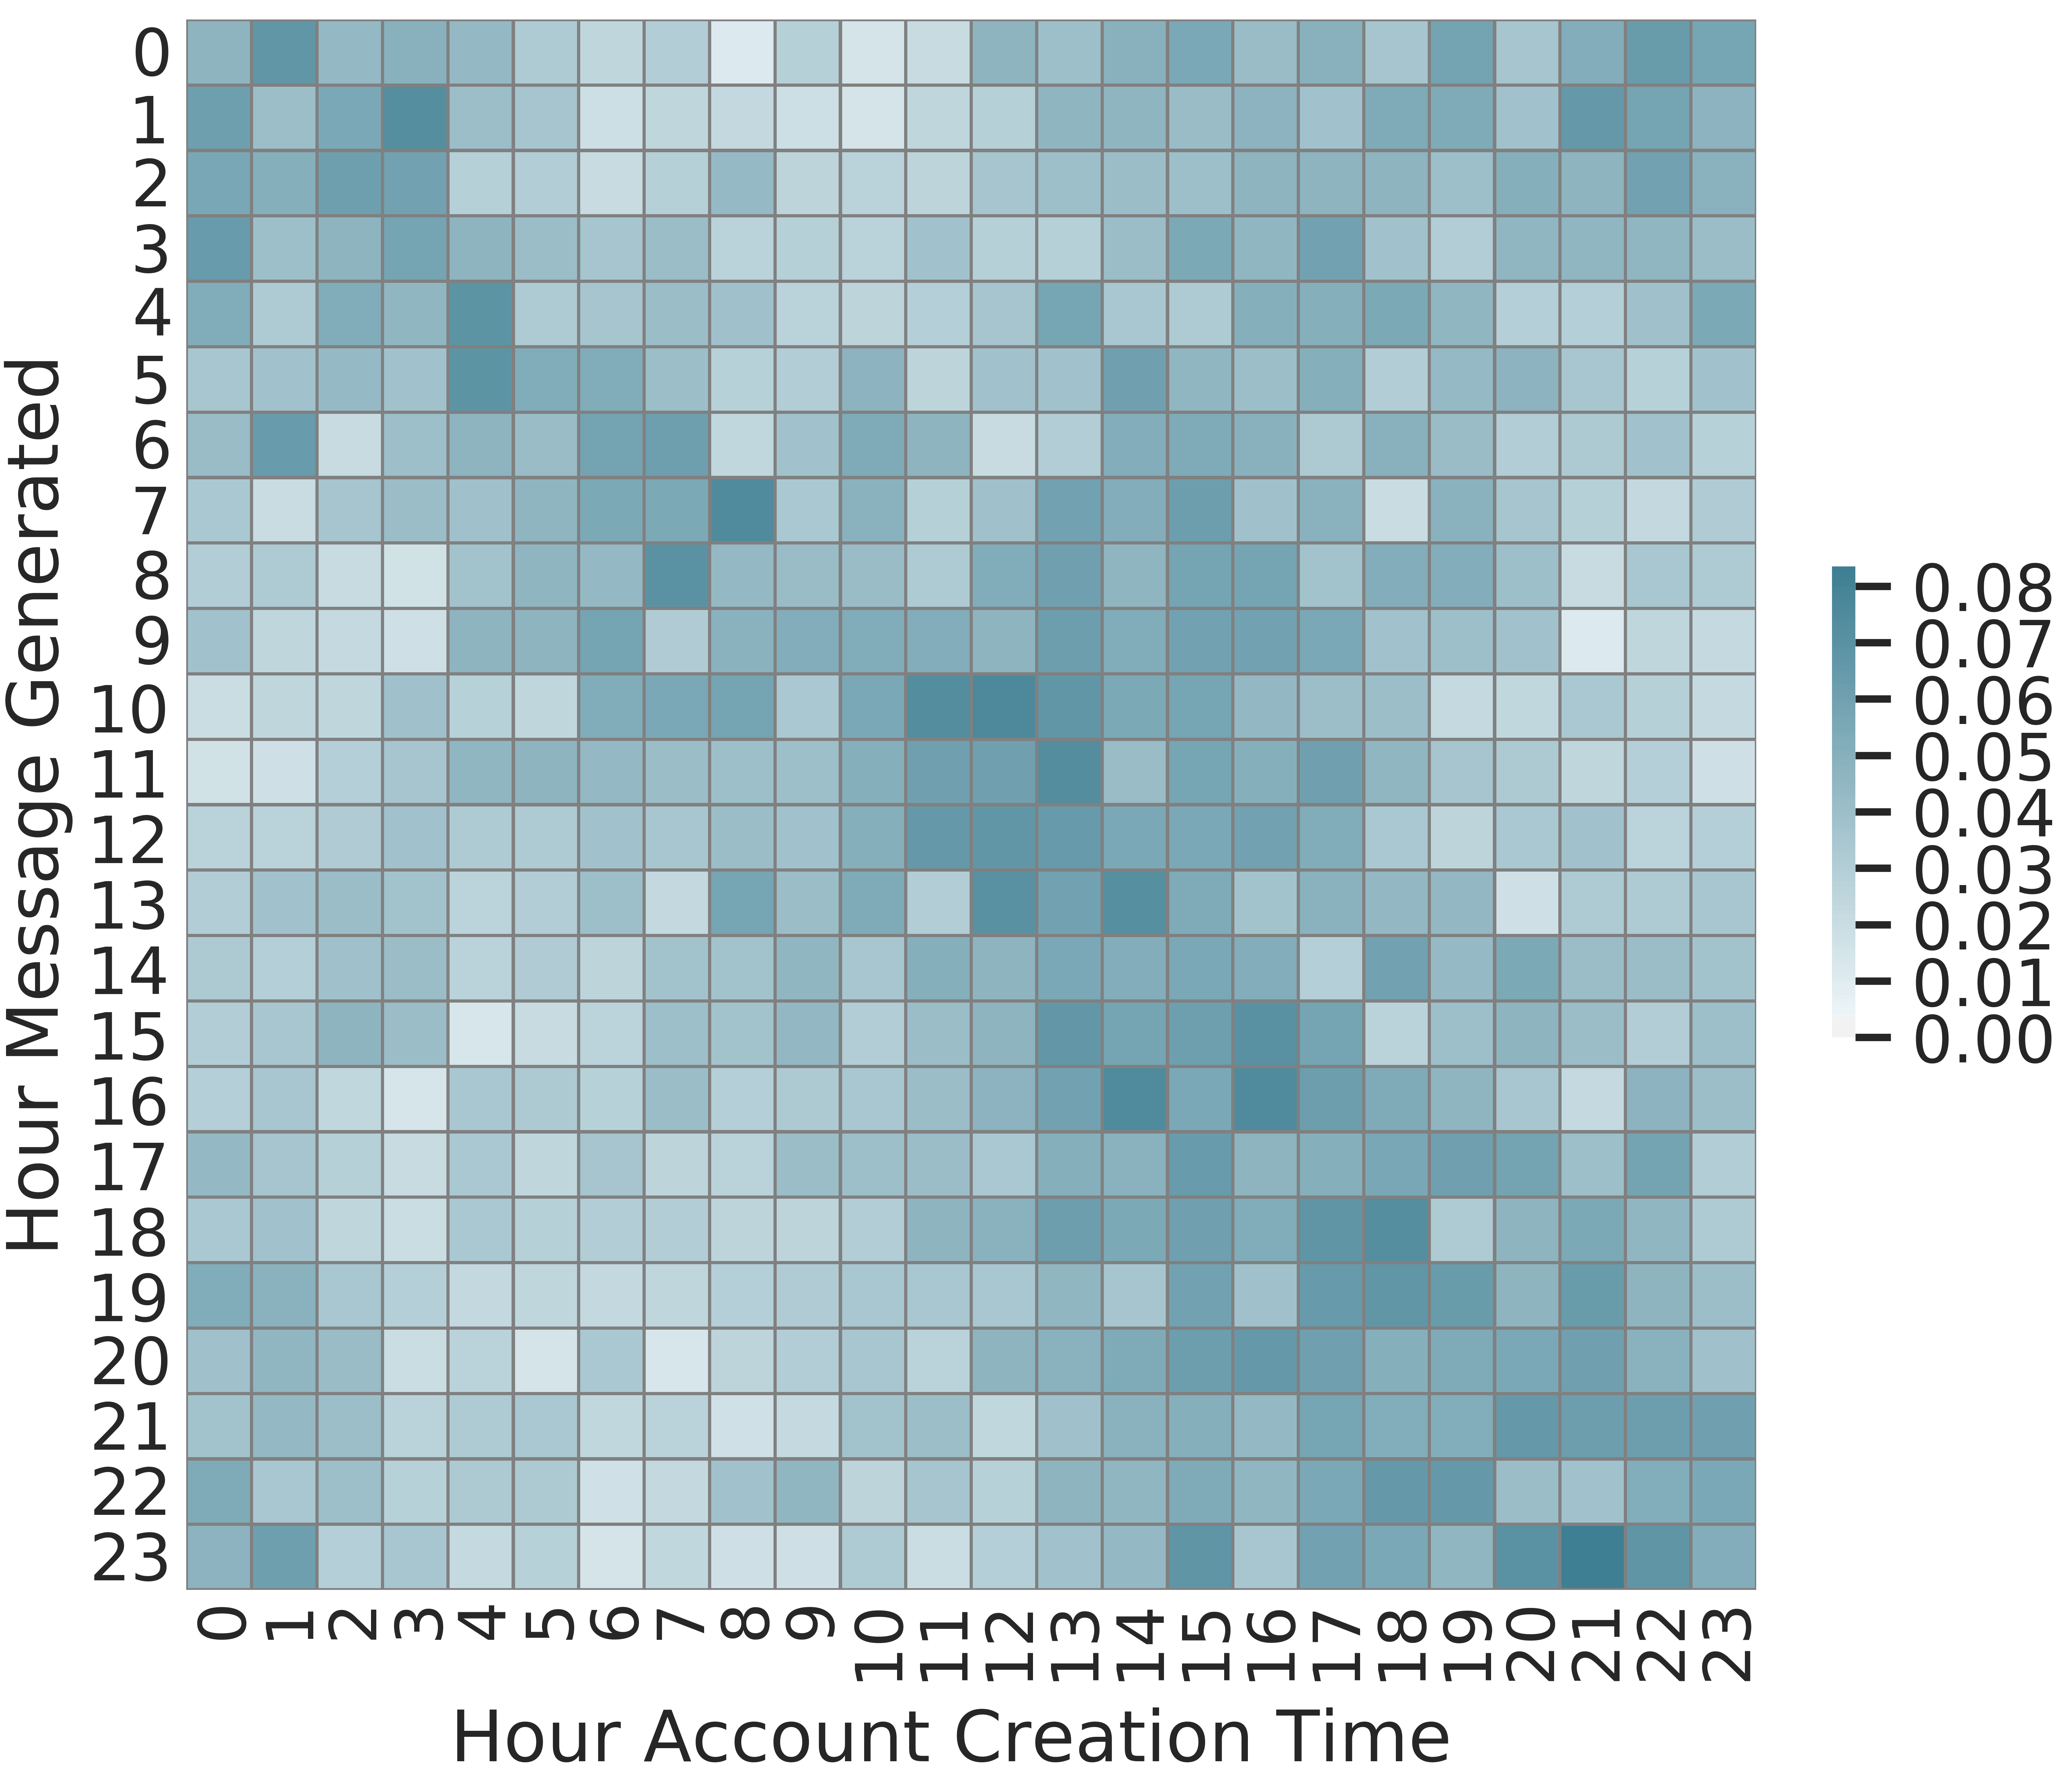
\includegraphics[width=.52\textwidth]{Figures/StackedDist@youtubeHeatmap2.png}}
   %\hspace*{\fill}   % maximize separation between the subfigures
   \subfloat[Messages with `trump']{\label{fig_Explanationb}
      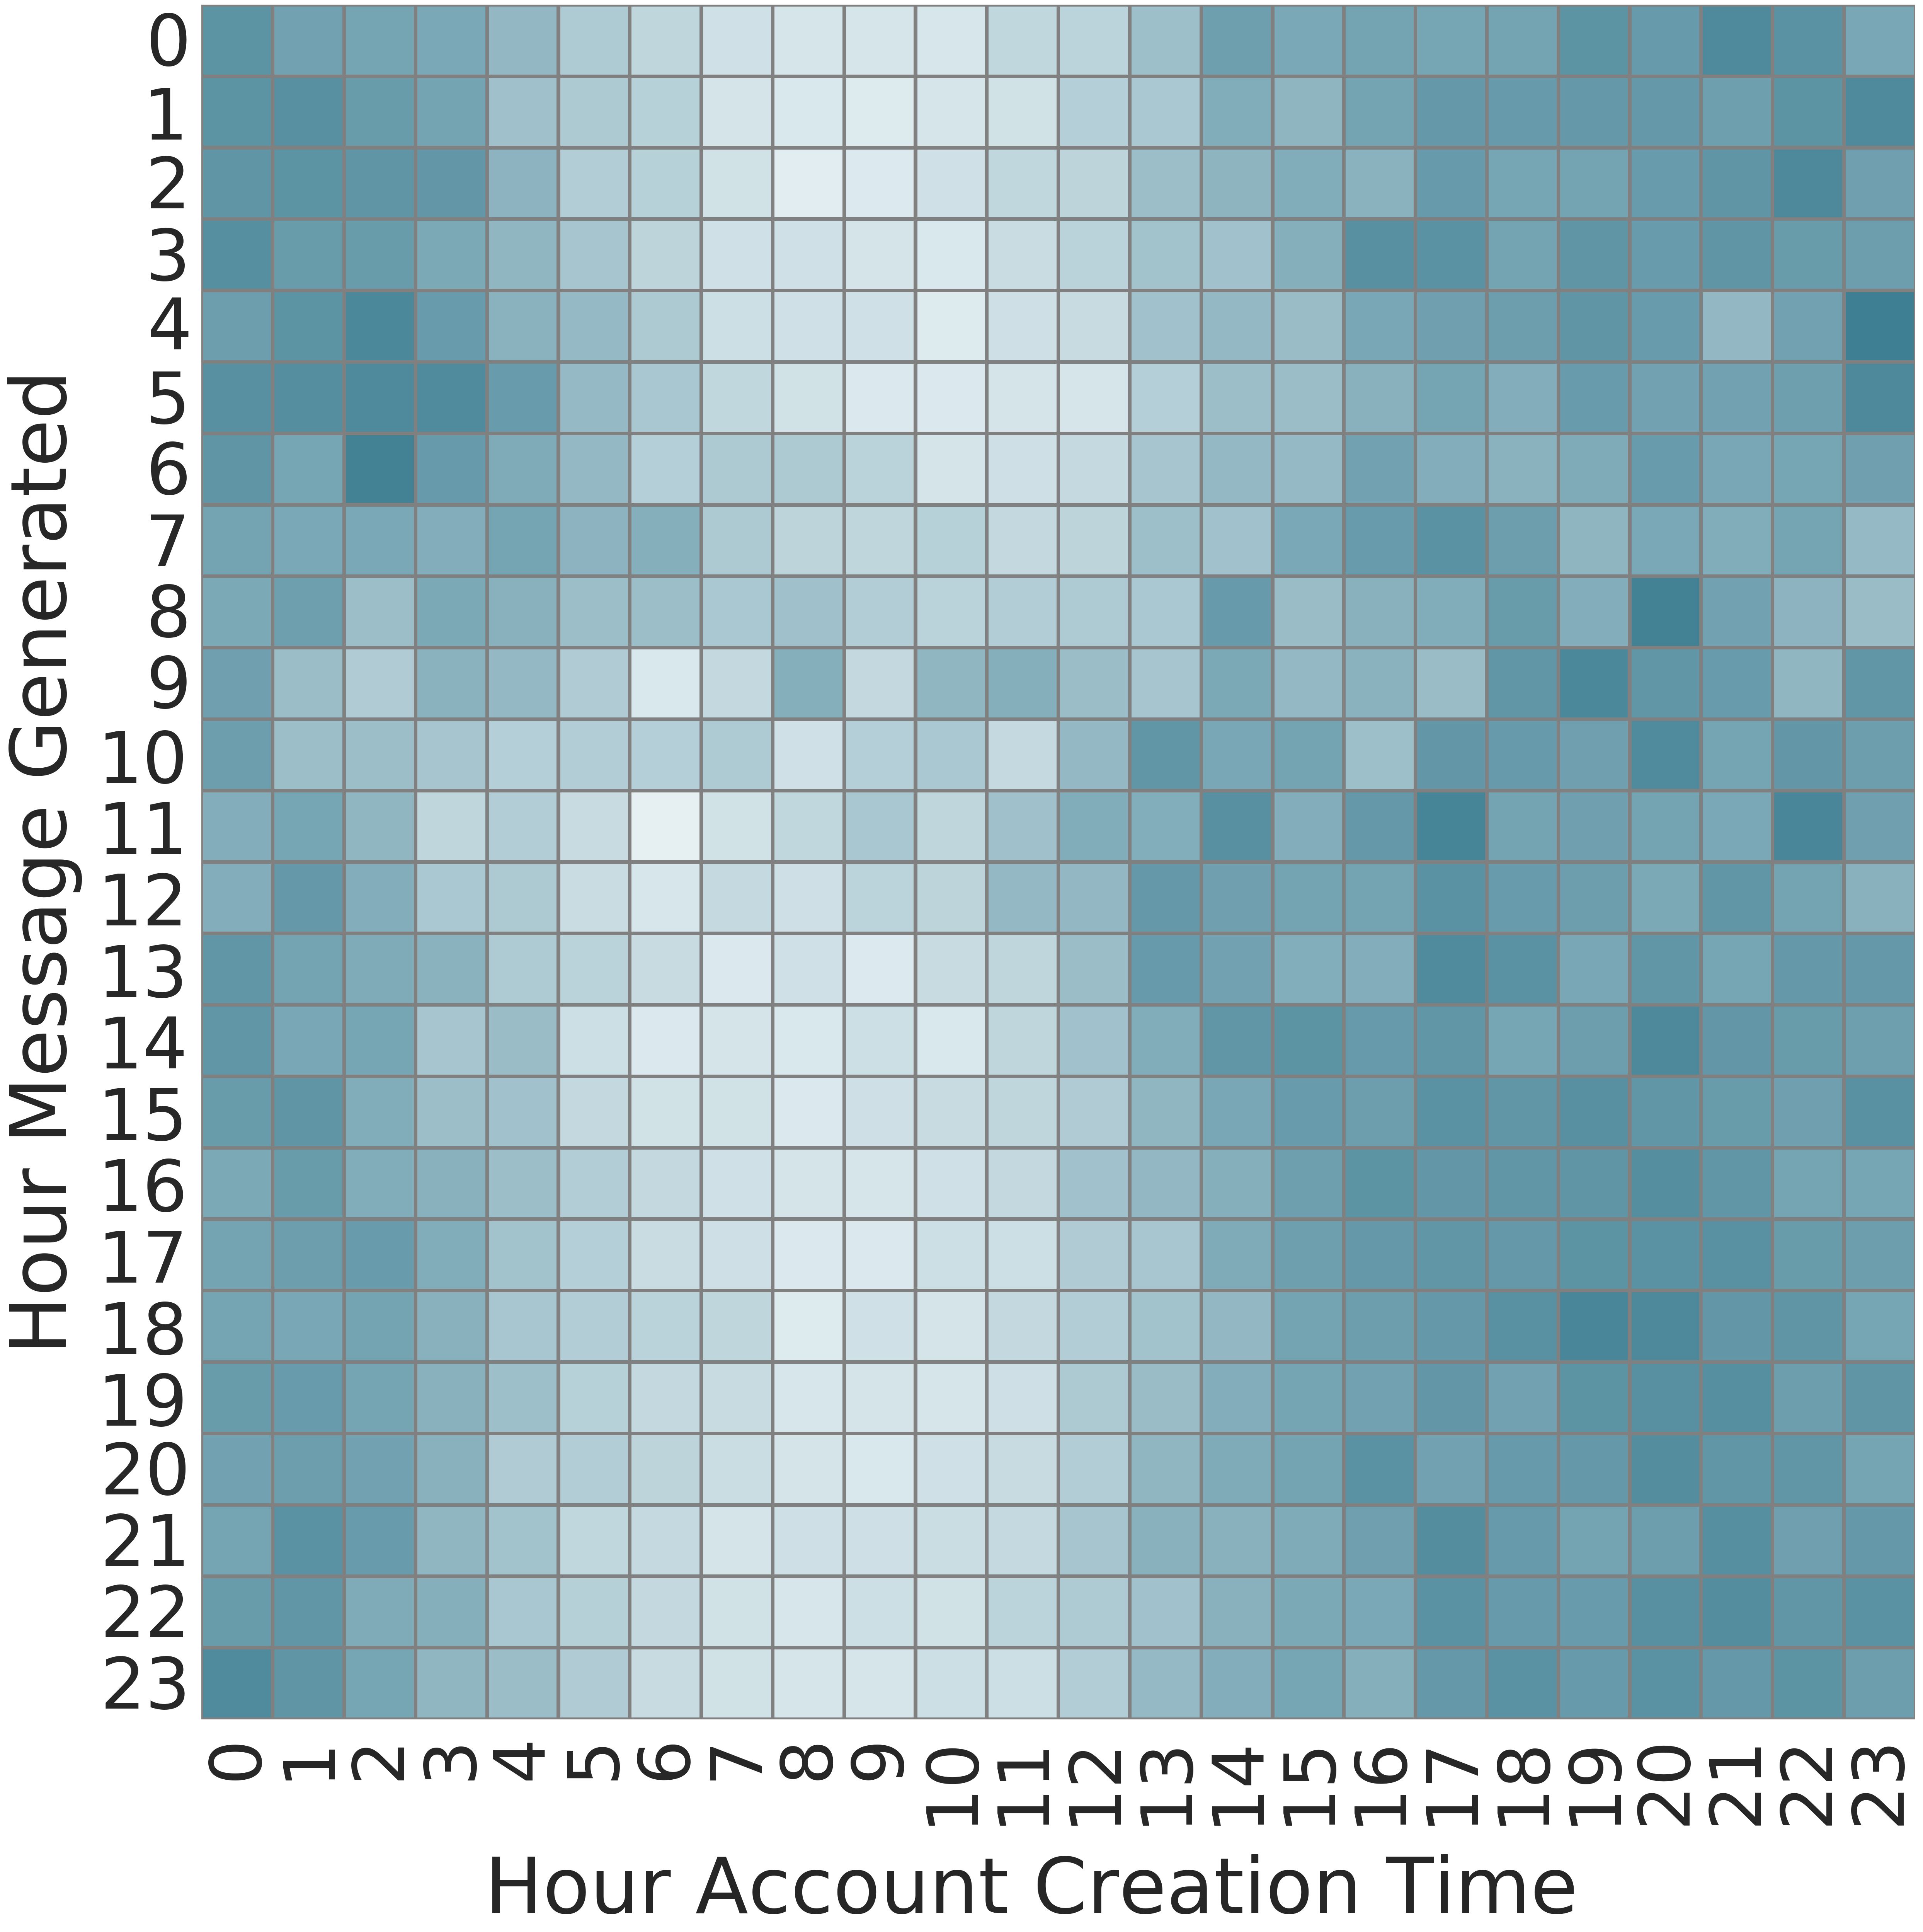
\includegraphics[width=.45\textwidth]{Figures/StackedDisttrumpHeatmap2.png}}
   \caption[Peak Analysis over Message Traffic]{Heat maps showing 24 time-distributions from users’ creation times where users are binned by the hour that they generated messages containing tokens: (a) `@youtube' 
   (global) and (b) `trump' (local). For a global token like `@youtube' we see that if a user was active in posting a message during hour $h$, then the user was likely to have created their account near the same hour $h$. For token `trump' a sleep cycle is observed (period of inactivity hours 5-11).} \label{fig_Explanation}
\end{figure*}

The distinction between global and local influencers is illustrated by comparing Fig. \ref{fig_Explanation}(a) vs. Fig. \ref{fig_Explanation}(b). Fig. \ref{fig_Explanation}(b) focuses on a more localized token 'trump' that clearly has a period of inactivity, a sleep cycle, during hours 5-11 (token has $c_2 > 0.001$ and during the collection period it was heavily discussed in the Americas). 

The concepts observed over message analysis apply to studying the influencer's followers. We do not know when a user followed an influencer, but because the followers are in sequence of follow time this indicates which followers must have followed earlier on. Algorithm 1 attempts to find a batch of followers of size $n$ that results in a unimodal distribution, which indicates that the followers are likely to have followed the influencer during the same hour as their account creation. When 24 batches, of size $n$, each peak during a different hour in sequence, it gives confidence that the follower gain around the 24-hour time period has been accurately identified (as has been illustrated in Fig. \ref{fig_3N} for followers of \emph{@CNN} and like the Identity Matrix in Fig. \ref{fig_Explanation}(a)).

Algorithm 1, for this reason, is well suited for global influencers that are gaining followers around the clock. In contrast, the heat maps for localized influencers show no strong peaks during some hours of the day. The approach, presented above, also cannot be relied upon for influencers that are gaining no more than 50 followers a day, because the average hourly batch will be too small to generate a meaningful time distribution. 

There will be periods during which an influencer gains no followers and even loses followers. We can reason only about followers that the influencer currently has, i.e., we cannot know which followers an influencer might have had in the past. If the influencer has lost many original followers, then the signal in the data will be obscured by considerable noise; $\rho$ will be small since the peaks will not cover all hours, and the order might not be perfect. Hence we have chosen to focus on influencers that have a large stable following and that are continuing to increase their follower base. It is preferable to pay close attention to $\rho$ and to stop making inferences after $\rho$ goes below some threshold. It is also recommended to compare the modified baseline based on Meeder et al. [\ref{appendix:5.15}] as an additional check against our method.

\subsection{Studying the Evolution of Popularity}

To study an influencer's evolution of popularity we need to find  how many followers the influencer has gained over multiple days. In an earlier subsection, we have shown that we can estimate an influencer's follower gain over past 24 hours. 
The same technique can be repeatedly applied to study the gains  over a longer time span. 

To understand the evolution of an influencer's popularity, we first find its followers' creation time list, $L_t$, obtained at time $t$. Unlike the list in the previous section that contained only 50K followers, this list consists of all available followers of the influencer. 

Say we have an influencer with 10 million followers. We could send the whole list to Algorithm 1, but it is not reasonable for the influencer to have gained 10 million followers in 1 day, and so to reduce computation we send a smaller more reasonable list. The feature $wSize$ sets the threshold for the maximum number of followers to send to Algorithm 1 (this threshold can be increased or decreased based on influencer's popularity).
 
 Using the first $wSize$ followers between indices [0, $wSize -1$] of $L_t$, Algorithm 1 calculates the number of followers gained %over one day (
 between $t$ and $t-1$, denoted as $p_{24}^t$. The next $wSize$ followers between indices: [$p_{24}^{t}$, $wSize + p_{24}^{t}-1$] will calculate $p_{24}^{t-1}$ (gain between $t-1$ and $t-2$). The next $wSize$ followers between indices: [$p_{24}^{t}+p_{24}^{t-1}$, $wSize + p_{24}^t+p_{24}^{t-1} -1$] will calculate $p_{24}^{t-2}$ (gain between $t-2$ and $t-3$). The daily gains returned as list: [$p_{24}^t$, $p_{24}^{t-1}$, $p_{24}^{t-2}$, ....] successively going backward in time.
 
 Using this approach with $wSize=50000$, Table \ref{table_5N} illustrates the number of followers gained in the last 10 days by two examples of qualitatively different kinds of influencers: \emph{@MrBeastYT} and \emph{@NPR}. The table also contains the associated correlation values (suggesting the degree of confidence), and the maximum number of unique hours captured by the peaks for each calculation from Algorithm 1. We observe that \emph{@MrBeastYT} consistently adds more followers %(per single period or cycle in chart) 
 than \emph{@NPR}. \emph{@MrBeastYT} also has higher unique hours and higher correlation, suggesting greater confidence in these predictions. This is reasonable since a more popular influencer will have more hourly followers, and consequently, the time distribution will be formed using more data points.
 
\begin{table}[htbp]
\small
\caption[Inferring Daily Follower Gains over 10 days]{Comparison of numbers of followers gained 
($p\textsubscript{24}\textsuperscript{t-d}$)
over each of 10 days by two influencers, along with correlation values maxP and the number of hours maxH spanned by the followers in each 24-hour period}
\label{table_5N}
\centering
\begin{tabular}{|c|c|c|c|c|c|c|}
\multicolumn{1}{c}{}  & \multicolumn{3}{c}{\bfseries \emph{@MrBeastYT}} & \multicolumn{3}{c}{\bfseries \emph{@NPR}}\\
\hline
\bfseries period t-d & \bfseries p\textsubscript{24}\textsuperscript{t-d} & \bfseries maxP & \bfseries maxH & \bfseries \bfseries p\textsubscript{24}\textsuperscript{t-d} & \bfseries maxP & \bfseries maxH\\
\hline
t-1 & 12480 & 0.989 & 20 & 1680 & 0.759 & 18\\
\hline
t-2 & 12120 & 0.993 & 21 & 1560 & 0.944 & 18\\
\hline
t-3 & 14400 & 0.98 & 22 & 1440 & 0.678 & 20\\
\hline
t-4 & 9480 & 0.98 & 22 & 1800 & 0.847 & 16\\
\hline
t-5 & 10800 & 0.989 & 23 & 1440 & 0.91 & 20\\
\hline
t-6 & 12960 & 0.934 & 20 & 1320 & 0.944 & 17\\
\hline
t-7 & 10800 & 0.981 & 21 & 1560 & 0.834 & 19\\
\hline
t-8 & 11520 & 0.978 & 22 & 1680 & 0.972 & 20\\
\hline
t-9 & 11520 & 0.979 & 21 & 1440 & 0.948 & 21\\
\hline
t-10 & 10440 & 0.984 & 22 & 1560 & 0.967 & 21\\
\hline
\end{tabular}
\end{table}

\begin{figure}[!htb]
\centering
\includegraphics[width=5.9in]{Figures/BeastVsNPR.png}
 \caption[Visualizing Daily Follower Gains]{Daily follower gains from the proposed method are shown as black tick lines on top for \emph{@NPR} and on the bottom for \emph{@MrBeastYT}. The cosine similarity curve, as described in text, has a periodicity that predictions from the proposed method can capture. We can thus visually verify that the proposed method is making meaningful predictions going backwards in time beyond a single day.}
\label{fig_7N}
\end{figure}

%Alternatively, 
The evolution of popularity for these two influencers can be visualized %, as 
using Fig. \ref{fig_7N}, % Figure is 
generated by repeatedly taking $n=200$ followers at a time. The $x$ value corresponds to the index of the last follower in the sample $[n, 2n, 3n,\ldots]$. Time distribution is formed over followers using indices $[x-n:x]$ and the hour during which time distribution peaks is recorded. The cosine similarity between the first peak hour vs. the sequence of all peak hours is recorded. 

The cosine similarity curve has a periodicity (it starts at 1 goes to -1 and then back to 1). The predicted $p_{24}^{t-d}$ from Table \ref{table_5N} %appear 
are shown using black tick lines at the top of the chart for \emph{@NPR} and the bottom for \emph{@MrBeastYT}. For example for \emph{@MrBeastYT} the black tick lines appear at [$p_{24}^{t}=12480$, $p_{24}^{t}+p_{24}^{t-1}=24600$, $p_{24}^{t}+p_{24}^{t-1}+p_{24}^{t-2} = 39000$, $\ldots$]. Visually we can see that the black ticks correspond to the periodicity of the curve for each influencer. In this way, another way to think about our method is in being able to capture the lengths of the periods in Fig. \ref{fig_7N}, which happen to correspond to the past number of daily followers gained. 

\section{Global vs. Local Influencer Classifier} \label{sec6}

In this section, we consider the problem of classifying local versus global influencers. For this, we generate a labeled dataset with 680 local and global influencers. The features are based on sleep cycle analysis (from Section 3.2) and peak analysis (from section 5.2). The resulting classifier illustrates that the features proposed in this chapter are well suited for the task.

\subsection{Dataset}

The method from [\ref{appendix:bookCh29}] is used to generate a list of global and local influencers. Automated Google search queries are utilized to get top Twitter influencers associated with the 100 most populous US cities. The followers of the top influencers are used to generate communities representative of each city. A modified TF-IDF algorithm is used to rank influencers based on whether they have a strong connection to a single city community (local) vs. multiple communities (global). Each influencer was verified manually by reading the influencer's description and other profile meta-data. In this manner, 680 influencers  were identified out of which 558 were local and 122 were global. 

\subsection{Features}

Given a new influencer, we  collect  the list $L_t$, of up to 50K followers. Next, Algorithm 1 is applied over $L_t$ to generate features: $p24$, $maxP$, and $maxH$ ($F_0$ to $F_{2}$  listed below). In the following, the temporal distribution, resulting from the first $p24$ followers in $L_t$ is denoted as $p24Dist$. 
\begin{enumerate}
\item $F_0=p_{24}$; if $p_{24} < 500$, $p_{24} = 500$.
\item $F_1=maxP$:  the associated $\rho$.
\item $F_2=maxH$; the maximum number of unique hours with peaks.
\item A quadratic is fitted over sleep cycle in $p24Dist$ (as described in section 3.2):

\begin{eqnarray*}
F_3 = \left\{
\begin{array}{ll}
c_2 & \mbox{if sleep cycle exists and quadratic is parabolic}\\
0 & \mbox{otherwise.}
\end{array}
\right.
\end{eqnarray*}
\item  $F_4=std(p24Dist)$, the standard deviation associated with $p24Dist$.
%\item $F_5$ to $F_{14}$ are top 10 Fourier Coefficients associated with $p24Dist$. \footnote{Complex Fourier transform was used with the SciPy mathematical Python library. The real coefficients corresponding to the cosine terms recorded.}
\item $F_5$= the fifth Fourier Coefficient (we tried the top 10 Fourier Coefficients\footnote{Complex Fourier transform was used with the SciPy mathematical Python library. The real coefficients corresponding to the cosine terms recorded.} associated with $p24Dist$, but the final classifier did not find others significant. A time distribution with a quadratic will need to be represented using higher order Fourier Coefficients, $F_5>0$. Conversely, a simple linear function can be represented using fewer coefficients so that $F_5==0$.
\end{enumerate}
 
\subsection{ Results -- Local versus Global Classification}
We use four families of classifiers:
\begin{enumerate}
\item Support Vector Machine (SVM) with the dot, radial, and polynomial kernels, 
\item Na\"ive Bayes, 
\item  Decision Tree; using information gain with max depth = 5, and 
\item Random Forest; the number  of trees $\leq 10$, each tree uses information gain with max depth = 5.
\end{enumerate}

Cross-validation with $K=5$ was employed. Accuracy is averaged over  5 iterations. Decision Tree gave the best results with an average accuracy of $(96.91\pm 1.08)$\%, followed by the Random Forest $(96.18 \pm 0.86)$\%, and Na\"ive Bayes $(96.18 \pm 1.27)$\%; SVM performed  poorly for all three kernels. The Decision Tree Classifier is shown in Fig. \ref{fig_decTree}.

\begin{figure}[!t]
\centering
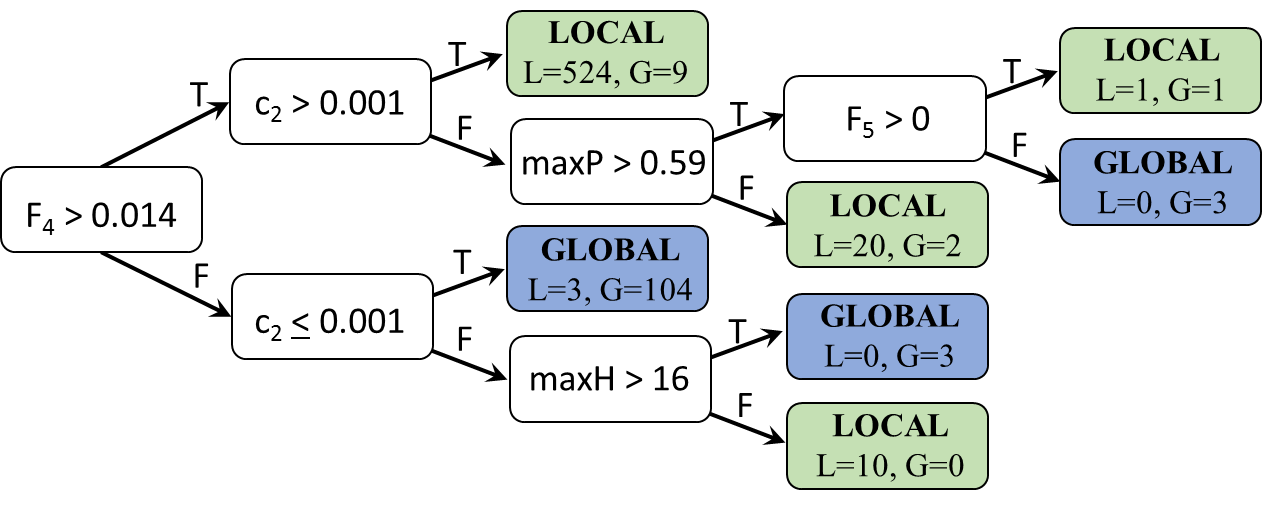
\includegraphics[width=5.9in]{Figures/DecisionTree.png}
 \caption[Global vs. Local Classifier]{Decision Tree Classifier for differentiating local vs. global influencers based on the features from account creation times of their followers. The number of local (L) and global (G) influencers predicted using each branch shown for each leaf node.}
\label{fig_decTree}
\end{figure}

\iffalse
The Decision Tree Classifier is shown below; after each branch the number of local (L) and global (G) influencers that end up as leaf nodes are shown:
{\fontfamily{pcr}\selectfont
\begin{tabbing}
in\=fluencer\_type\_decision\_tree($F_1$, $F_2$, $F_3$, $F_4$, $F_5$):\\
\> $F_4$ $(std(p24Dist))$ $> 0.014$: \\
\> |-- $F_3$ $(c_2)$ $> 0.001$: Local (L = 524, G = 9)\\
\> |-- $F_3$ $(c_2)$ $\leq 0.001$: \\
\> |-- |-- $F_1$ $(maxP)$ $> 0.590$: \\
\> |-- |-- |-- $F_5 > 0$: Local (L = 1, G = 1) \\
\> |-- |-- |-- $F_5 \leq 0$: Global (L = 0, G = 3) \\
\> |-- |-- $F_1$ $(maxP)$ $\leq 0.590$:  Local (L = 20, G = 2) \\
\> $F_4$ $(std(p24Dist))$ $\leq 0.014$: \\
\> |-- $F_3$ $(c_2)$ $> 0.001$:  \\
\> |-- |-- $F_2$ $(maxH)$ $> 16$: Global (L = 0, G = 3) \\
\> |-- |-- $F_2$ $(maxH)$ $\leq 16$: Local (L = 10, G = 0) \\
\> |-- $F_3$ $(c_2)$ $\leq 0.001$: Global (L = 3, G = 104) \\
end \\
\end{tabbing}
}
\fi

We used information gain to rank the features.  Top four features and their associated weights are:(i) $F_1$: 1, (ii) $F_4$: 0.983, (iii) $F_2$: 0.972, (iv) $F_3$: 0.956 (the weight for $F_5$: 0.058 so it is not as significant).

 As we have seen in the previous section, a sample of followers from a global influencer can lead to a time distribution that is unimodal, and for this reason, it is important to take a sample determined by Algorithm 1. Algorithm 1 searches for the optimal curve that is achieved if the peaks from time distributions are in sequence and contain all 24 hours; if the $\rho$ ($F_1$) is low and if a small number of hours ($F_2$) are covered this indicates a local influencer. 
%Based on the analysis of decision tree we note that 

If $F_4$ $(std(p24Dist))$ is low then the spatial  distribution is flat and belongs to a global influencer; which is consistent with observations made in the previous sections. The information gain identified that $F_3$ ($c_2$) less than 0.001 should be the cutoff for a global influencer (this exact value was also confirmed from analysis of stop words using message traffic in Section \ref{sec4}). Finally, if the time distribution is represented using only low order Fourier coefficients so that $F_5=0$ this means this is more of a flat line simple time distribution associated with a global influencer. %($FC_1$ had higher initial information gain, but after other features considered decision tree utilized $FC_4$).

This classifier is intuitive and over the whole dataset achieves 665/680 = 97.79\% accuracy. The followers of influencers that the classifier predicts as local %such as \emph{@BBCRussian} 
can be used for predicting UTC offset related to local expert finding in social networks. While the followers of global influencers %such as \emph{@BBC\_Travel} 
can be used for inferring daily follower gains and analyzing how their popularity has evolved.

\section{Conclusions} \label{sec7}

In this chapter, we have illustrated an approach for how creation times can be used in time series analysis. The creation times can stem from a group of messages or account creation times. It was illustrated that the distribution of creation times that stem from a single time zone %will form a time curve with a U-shaped valley. The U-shape 
will be approximately %paraboloidal
parabolic, with a minimum during the night time for that %corresponds to the time that the 
time zone. % experiences night. 
%By fitting a second degree polynomial the U-shape 
Regression with a quadratic function can be used to predict the UTC offset associated with the time zone. 
By examining message traffic, this information was utilized to identify trending keywords over %any
multiple geographic %area
areas of interest. 
In addition, by analyzing the set of followers of any influencer, we showed that this information can be utilized to determine how strongly localized is the range of influence
of an influencer. % is localized.
%to area of interest. 
This is useful for Location-Aware Influence Maximization (LAIM) and local expert finding in social networks. 

%By taking x followers at a time it was 
We also illustrated that a follower sample exists such that the peaks from multiple time curves occur in sequence. 
Analysis of variations of %the peaks %By plotting the peaks 
the wave pattern in the distribution of peaks
provides information %for studying
regarding the periodicity with which followers were gained. This is useful for understanding how an influencer's popularity has evolved over time, as well as for inferring link creation times.%, i.e.,   when a set of followers mentioned the influencer.

Finally, the proposed time-based features were utilized for creating a local vs. global type classifier. The classifier is important because the UTC offset prediction should be applied for local influencers whereas the analysis for how influencer's popularity evolved %over time 
works for global influencers.

\graphicspath{{Paper5Figures/}}
\chapter{Application 1: Multilingual Geocoder based on labels using Time and Language Features}\label{chap:ch6}

\section{Introduction}
As has been shown in Chapter 2, it is inherently difficult to build a universal geocoding solution that can handle various languages and their associated alphabets, popular slang, and purposely ambiguous phrases on Twitter. In a step towards a universal geocoding solution, Chapter 5 showed that time-based features could be used for identifying whether the user group is from a particular timezone. A timezone spans a large geographic area, but the language features can constrain the set of possible countries. In this chapter, the proposed approach is illustrated by categorizing 320K Twitter influencers. High confidence influencer predictions are used as training data for an improved geocoder. This geocoder automatically learns popular ways that Twitter users refer to locations within the country and can handle foreign alphabets.

\section{Influencers-Dataset}

In this dataset, user groups are binned by the influencer they follow. The influencers for the dataset were chosen from the special Twitter \emph{@verified}. It tracks all influencers that have passed an internal Twitter check (after Twitter performs a special check the influencer is identified via a special blue badge). In this dataset, collected in the spring of 2019, there are 320,166 influencers. Due to Twitter API limits, for each influencer only a single API call was made which returned at most 5000 followers.

The ground truth consists of the country associated with the self-reported location reported by the influencer. It is checked whether this country can be used as a label, based on whether this country matches (i) the most frequent country from self-reported locations of followers and (ii) whether it is contained within the set of countries that would be predicted using followers' time and language features. It is shown that time and language features can be used to improve the precision of the country labels. The country label and the associated influencer's followers' self-reported locations are used for training and illustrating a multilingual geocoder. 

\section{Incorporating Language} 
We utilize language to further improve the performance of the time-based classifier proposed in section 5.3. Given a time distribution associated with a user group we can compute $UTC^P$ (equation (5.2)). Let $U_1$ equal the set of countries whose cities have a time zone that observes UTC offset in the range $[UTC^P-t_1 , UTC^P + t_1]$, where $t_1$ is a preselected threshold.  For example,  the set of countries [TLS, PLW, JPN, MNP, FSM, GUM, IDN, AUS, PRK, RUS, KOR, PNG], correspond to UTC range $\in$ [8, 10].

Our next step is to incorporate language information to constrain the set of possible countries for the selected UTC offset range. Initially, the CIA World Factbook was utilized for this purpose. But for some countries, the languages from CIA World Factbook did not align with the languages used on Twitter. For example, English is the most popular language in India for communication, but it does not make it into popularly spoken languages (instead Hindi, Bengali, and others are listed).

We utilized language preferences, a user-selected option, which is available for more than 99\% of collected users on Twitter. In our dataset, there are 76 unique language codes associated with 143 countries, each language was used by at least 100 users, collected over 373 million user profiles. 

Given a user group, the users' language preferences are used to generate a language distribution, i.e., we calculate:

\[ g_G(\ell) = \frac{\text{\# of users of language } \ell \text{ in } G}{|G|}\]
for all 76 languages. The language distribution for all countries was also calculated, i.e.,

\[ h_c(\ell) = \frac{\text{\# of users of language } \ell \text{ in country } c}{\text{\# of all users in country } c}\]
for all 143 countries.

Using cosine similarity  $g_G(\ell)$ is compared with  $h_c(\ell)$ for all 143 countries. Let $U_2$ be the set of countries whose language distributions have a similarity score greater than threshold $t_2$. Finally, let $U_3 = U_1 \cap U_2$ that is, $U_3$ equals the set of countries common to both sets $U_1$ and $U_2$.

Table \ref{table_4app} shows how the language distributions helps narrow down the list of possible countries for different thresholds $t_2$. Recall that for each user group in the UTC offset dataset its location and therefore its country is known. For each user, if this country is in set $U_i$ then the prediction is marked correct, incorrect otherwise. In Table \ref{table_4app} the first three columns are the median number of countries associated with $U_1$, $U_2$, and $U_3$. 

\begin{table}[htbp]
\small
\caption[Constrain set of possible countries via language]{Language helps constrain the set of possible countries from UTC while improving precision for higher cosine similarity, $t_2$}
\label{table_4app}
\centering
\begin{tabular}{|c|c|c|c|c|c|}
\hline
\bfseries U\textsubscript{1} & \bfseries U\textsubscript{2} & \bfseries U\textsubscript{3} & \bfseries P & \bfseries R & \bfseries t\textsubscript{2} \\
\hline
19 & 143 & 17 & 89.02 & 100.00 & 0.05 \\
\hline
19 & 140 & 17 & 89.14 & 99.87 & 0.15 \\
\hline
19 & 127 & 12 & 89.54 & 99.42 & 0.25 \\
\hline
19 & 115 & 8 & 89.75 & 99.18 & 0.35 \\
\hline
19 & 108 & 7 & 90.07 & 98.80 & 0.45 \\
\hline
19 & 102 & 7 & 90.23 & 98.58 & 0.55 \\
\hline
19 & 99 & 6 & 90.32 & 98.38 & 0.65 \\
\hline
19 & 91 & 6 & 90.27 & 98.23 & 0.75 \\
\hline
19 & 83 & 5 & 90.26 & 97.84 & 0.85 \\
\hline
19 & 70 & 4 & 90.34 & 96.01 & 0.95 \\
\hline
\end{tabular}
\end{table}

It can be seen that our final prediction, identified by the set $U_3$, has good accuracy and a much smaller set of possible countries then initial $U_1$. From table, values from 0.85 to 0.95 work well for $t_2$.

\section{Illustration over Influencers-Dataset}
The prediction methods, discussed in previous sections, are shown in a pipeline in Fig. \ref{fig_6app}. As an application, the pipeline is applied over Influencers-Dataset. The goal is to identify geo-influencers and accurately associate them with the country that most of their followers are from. We are interested in high confidence influencer predictions because these in turn can be used as training data for a multilingual geocoder that will be presented in the following section. 

\begin{figure}[h!]
\centering
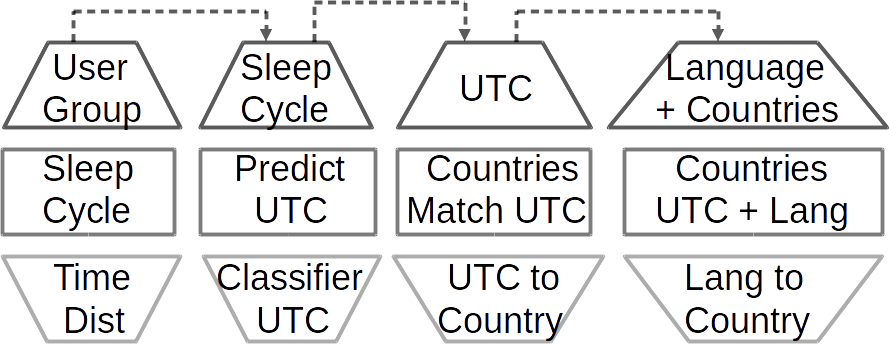
\includegraphics[width=4.5in]{FigA882}
\caption[Pipeline for predicting region of the world]{Pipeline for predicting region of the world using time and language features. The top layer shows input, the middle layer output, and the bottom layer the name of the process. Each step sends its output as input to the next step.}
\label{fig_6app}
\end{figure}

One data point is the influencer's self-reported location. Another data point is the ratio of followers' self-reported locations belonging to a particular country. The expectation is that for geo-influencers the country associated with the self-reported location will match the most frequent country from influencer's followers. Self-reported locations that match a known GeoNames entry are utilized as described in section 5.3.1.

A problem with self-reported location information from followers is that the labeled location focuses on the Latin alphabet with foreign city names appearing as they would be referred to by an English speaker (Moscow instead of Moskva in Cyrillic). Therefore, English-speaking users are incorporated more often than non-English speakers. Using the following steps we aim to test the different stages from Fig. \ref{fig_6app} to help with this imperfect baseline:

\begin{enumerate}
\item Step 1a (S1a) -- Get rid of influencers whose followers' time distribution does not exhibit a U-shaped parabola.
\item Step 1b (S1b) --  Get rid of those influencers which are classified as global.
\item Step 2 (S2\_$t_1$) -- $UTC^P$ computed and used to obtain the set of possible countries $U_1$.
\item Step 3 (S3\_$t_2$) -- Reduce  the set $U_1$ to set $U_3$ by constraining to countries that have cosine similarity above $t_2$.
\end{enumerate}

Steps S1a and S1b should reduce the dataset to focus primarily on geo-influencers whose followers are concentrated in a single time zone. Steps S2\_$t_1$ and S3\_$t_2$ help identify and correct instances where the baseline is making poor predictions that do not match using countries based on time and time+language features, respectively. If the top-ranked country from the baseline is within the set of countries it is returned as a prediction otherwise the second top country is used and so on. 

There were 100,712 influencers with a self-reported location that could be resolved using GeoNames. The country that the influencer associates themselves with is used as ground truth. For example, \emph{@BBCNews} has a self-reported location `London' which is associated with GBR using GeoNames. 
Ordering by the most frequent country from followers' self-reported locations, the top five countries and associated percent of self-reported locations are USA: 28.15\%, NGA: 10\%, IND: 6.3\%:, GBR: 5.92\%, and KEN: 4.81\%. Thus, USA is the top prediction used in baseline, but this does not match the set of possible countries from S2\_$t_1$ and so NGA is used as it is the second best prediction; NGA has the same UTC as GBR and is thus within the set of possible countries using time features. Language features from S3\_$t_2$ can further constrain the prediction to the expected result, GBR.

In the above, we have described a procedure that results in a set of possible countries making up $U_3$. We also consider a point estimate prediction where a single country with the best cosine similarity is returned for a narrow UTC range $t_1=0.25$ (this point estimate is denoted as S3\_Point in Table \ref{table_5app}).

Table \ref{table_5app} shows how the baseline is constrained using each step of the pipeline. The second column shows precision across all influencers (100,712) and the fourth column shows precision across influencers not associated with the USA (37,908).

\begin{table}[htbp]
\small
\caption{Different Stages of Pipeline Improve Baseline Precision}
\label{table_5app}
\centering
\begin{tabular}{|c|c|c|c|c|}
\hline
& \bfseries All P & \bfseries Count & \bfseries Foreign P & \bfseries Count\\
\hline
Baseline & 86.34 & 100708 & 65.71 & 37904 \\
\hline
S1a & 86.23 & 95500 & 65.61 & 36087 \\
\hline
S1b & 89.98 & 71643 & 76.97 & 28725 \\
\hline
S2\_1 & 90.23 & 70544 & 77.39 & 28018 \\
\hline
S2\_0.5 & 90.95 & 65708 & 78.98 & 25845 \\
\hline
S2\_0.25 & 92.23 & 60387 & 79.43 & 20753 \\
\hline
S2\_1+S3\_0.95 & 91.49 & 64940 & 78.15 & 23315 \\
\hline
S2\_0.5+S3\_0.95 & 92.78 & 57584 & 80.86 & 19721 \\
\hline
S2\_0.25+S3\_0.95 & 94.54 & 50978 & 80.94 & 13395 \\
\hline
S2\_0.25+S3\_Point & 97.2 & 35518 & 86.59 & 6587 \\
\hline
\end{tabular}
\end{table}

Table \ref{table_5app} illustrates that as time and language constraints are added the precision improves. Removing influencers that don't pass the sleep cycle test surprisingly doesn't help (row S1a), but getting rid of influencers with noisy PST predictions (row S1b) results in a big jump in precision.% (both measures are related to focusing on geo-influencers which are expected to have a strong follower concentration in a single geographic area). 
UTC offset information further constrains the baseline (rows S2\_$t_1$). 
%{The smaller the $t_1$ the smaller is the geographic area that needs to be matched using baseline. }
The highest precision is achieved when both UTC and language information are used. 

\section{Training Geocoder with Support for Foreign Languages}

As already noted, the issue with the baseline Geocoder was that it handles only English based locations that have a match to GeoNames. Our proposed approach is to use the high confidence influencer predictions from the previous section as training data for an improved geocoder. This geocoder will automatically learn common ways persons refer to locations in their native tongue. 

This new geocoder is based on a TF-IDF model, where the country is the document and the terms are the self-reported locations of the influencer's followers. It is possible to apply this model because if the influencer and their followers belong to the same country, then the followers' locations will capture common ways persons refer to locations within that country. TF-IDF vectors are generated using the Gensim package in Python\footnote{https://radimrehurek.com/gensim/}. 

\iffalse
From equation \eqref{eq122}, the weights of TF-IDF are based on the frequency of term $i$ in document $j$ times log inverse ratio of total documents with the term over total $D$ documents. 
\begin{equation}
TF-IDF_{i,j} = frequency_{i,j}*log_2\frac{D}{doc_{freq_i}}\label{eq122}
\end{equation}
\fi

Focusing on the top $K$ TF-IDF features per country it is possible to verify that the model is generating reasonable vectors. Fig. \ref{fig_7app} shows the top three features for several countries. These strings capture typical ways persons refer to locations within that country which can serve as useful features for geocoding type classifiers. The model also helps confirm that the countries, with which the influencer's followers were associated with, are indeed relevant.

\begin{figure}[!t]
\centering
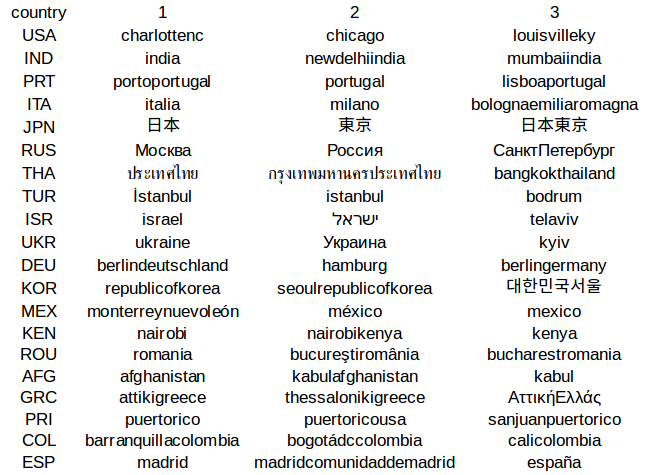
\includegraphics[width=4.7in]{FigA7}
\caption[Features from Multilingual TF-IDF Geocoder]{Top three TF-IDF location features automatically learned from country documents. The benefit of this model is that it learns popular ways of referring to the country's locations in different languages and will include common phrases, abbreviations, and so on.}
\label{fig_7app}
\end{figure}

Given a new influencer, the self-reported locations associated with the influencer's followers form a new document. A TF-IDF vector is built using self-reported location frequencies and the IDF component previously computed over the corpus of $D$ documents. Cosine similarity is then used to return the country vector that is closest to the TF-IDF vector. Because the TF-IDF vectors may be very large, we recommend utilizing Latent Semantic Analysis (LSA) to reduce dimensionality to at most 500 terms (from literature 50-500 is recommended as a standard [\ref{appendix:6b.17}]). Fig. \ref{fig_78app} highlights the overall approach. 

\begin{figure}[!t]
\centering
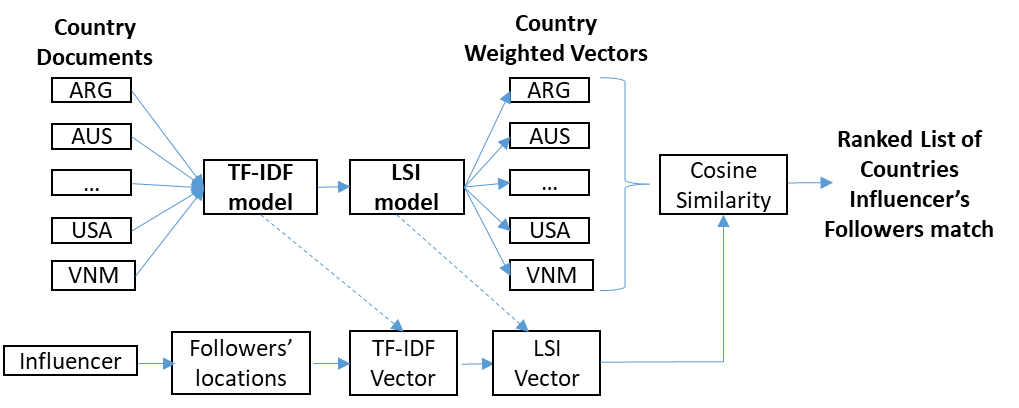
\includegraphics[width=5.7in]{FigA88}
\caption[Training TF-IDF Geocoder]{The process by which TF-IDF model is learned from geo-influencers associated with a country and used for predicting other geo-influencers.}
\label{fig_78app}
\end{figure}

In Table \ref{table_6app}, the performance of the TF-IDF model is shown against the baseline from the previous section. TF-IDF model has a higher precision than original baseline with a clear jump in precision for foreign countries. This improved geocoder can be used to generate labels across additional influencers (that could not be predicted using the original baseline). The additional labels can be verified using time and language features and the TF-IDF model can be further improved. The process can repeat until the process converges, that is, when the TF-IDF model no longer improves.

\begin{table}[htbp]
\small
\caption{TF-IDF model performance for Different Stages of Pipeline}
\label{table_6app}
\centering
\begin{tabular}{|c|c|c|c|c|}
\hline
& \bfseries All P & \bfseries Count & \bfseries Foreign P & \bfseries Count\\
\hline
Baseline & 86.34 & 100708 & 65.71 & 37904 \\
\hline
TF-IDF model & 88.44 & 100711 & 81.75 & 37907 \\
\hline
\end{tabular}
\end{table}

\section{Conclusions}
This chapter showed an application by which the geographic region can be labeled using only time and language features. The benefit of our approach is that these time and language features are universal and can be used across the whole Twittersphere. The labels have been used to train a high-level geocoder that has multilingual support. The benefits are that the common ways that Twitter users report their locations are captured by this geocoder. The drawback to our method is that it works at a high level for predicting regions of the world at the country level or larger. We envision that the features proposed will be utilized for augmenting with other features as part of information fusion.
\graphicspath{{repositoryFigures/}}
\chapter{Application 2: Repository of Influencers for Content Recommendation}\label{chap:ch7}
\section{Introduction}

As discussed in previous chapters, a repository of location-aware influencers may be of interest for content recommendation and for studying location related communities from influencer's followers. This chapter describes the repository collected as part of this research, the features, and the visualization we employ. The repository consists of over three hundred thousand verified influencers that are tracked by \emph{@verified}. For each user, the location information, time, and language features are recorded as was described in chapters 2, 5, and 6, respectively. Additionally, other demographics such as gender and race are considered. %Such a repository could be used for (i) content recommendation, (ii) to build communities around the followers of influencers that are known to serve a specific geographic location, and other applications. 

\section{Related Research}
Popular variables associated with demographics are geographical location [\ref{appendix:1.3}], age [\ref{appendix:4.2}], gender [\ref{appendix:4.3}], education [\ref{appendix:4.4}, \ref{appendix:4.5}], income [\ref{appendix:4.6}], ethnicity [\ref{appendix:4.7}], and others. Typically, due to privacy concerns, these variables are not specifically stated. However, by fusing information with other sources, it is possible to characterize a group of users with a certain level of confidence. For example from the US Census Bureau's Genealogy Project which publishes the frequency of popular surnames with their distribution per race/ethnicity, it is possible to characterize the percent of users that belong to a certain ethnic group [\ref{appendix:4.7}]. A lot of the approaches deal with English-speakers [\ref{appendix:4.8}].

Many additional variables may be inferred from online connections a user has that apply to any language. For example followers of @ESPN and @SportsCenter are more likely to be male, followers of @PlayStation are more likely to be kids, and followers of @ParentsMagazine are likely to have kids [\ref{appendix:4.9}]. Political orientation may be discovered by whether the user is connected to known political representatives [\ref{appendix:4.10}]. Timezone and language can be used for differentiating between countries. Our goal is to focus on those demographic features that can be used to characterize a large portion of the global population. Our repository focuses on self-reported location, gender, race, language, and time of the day their account was created. 

\section{Setting up the Repository}

Implementation utilized Ubuntu 16.04 as the OS, Python 3.5 as the programming language, and MongoDB 3.6.5 as the NoSQL database. %The repository is stored in folders for MongoDB and Eclipse workbench. An instance of MongoDB and Eclipse simply need to point to the folders. For example, on Ubuntu, the command: mongod --dbpath `path' would point MongoDB to a specific folder. Specific Python libraries such as pymongo for interfacing with MongoDB are installed via pip. 
ElasticSearch and Kibana were used to search and visualize data of interest.

\begin{figure}[htbp]
\centerline{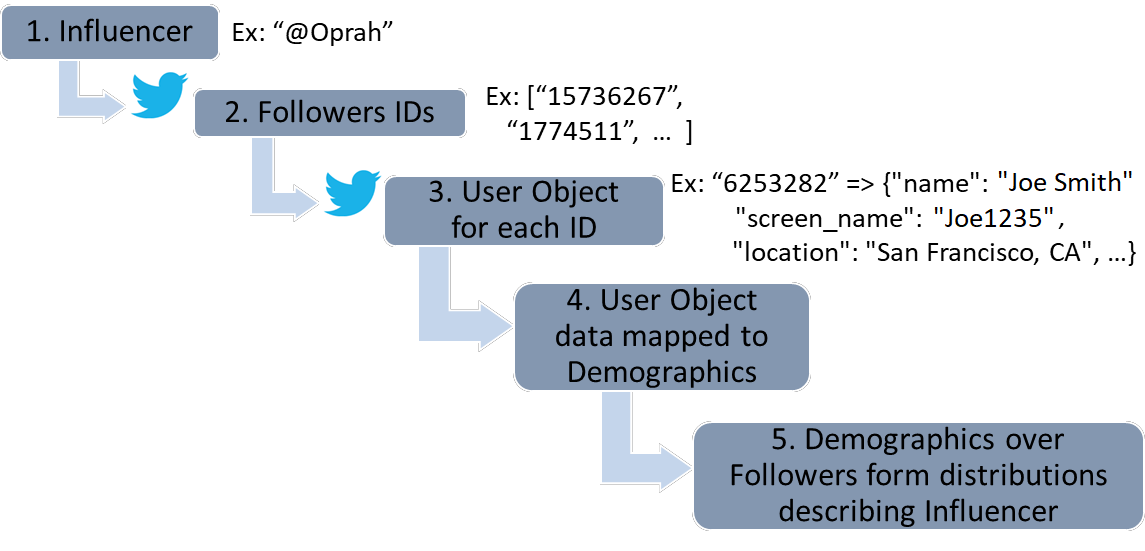
\includegraphics[width=4in]{Fig1.png}}
\caption{Collection Process.}
\label{fig_ch7_1}
\end{figure}

Fig. \ref{fig_ch7_1} illustrates the collection process for a single Twitter influencer. %The repository covers all of the Twitter influencers verified by Twitter. 
Each component from Fig. \ref{fig_ch7_1} is described below.

\begin{itemize}
\item Influencer to Follower IDs: influencers are identified from @verified. For each influencer, up to 5000 followers are collected. %We have seen that typically around 500 followers form a large enough sample to reason about influencer's demographics (for this reason and due to Twitter API limits for many influencers it is enough to collect at most 5000 followers). The connections between influencer to follower are stored in Twitter{\_}Connections database.

\item IDs to User Objects: Fig \ref{fig_ch7_2} is a Snapshot of our database. Database stores all followers and all influencers collected in tables `userInfo' and `followerInfo' respectively. Example of User Object from userInfo table shown in Fig \ref{fig_ch7_3}.

\begin{figure}[htbp]
\centerline{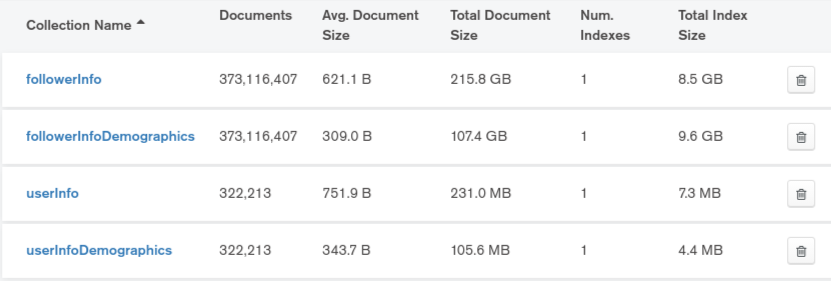
\includegraphics[width=5in]{Fig2.png}}
\caption[Database holding Twitter User Objects]{Database holding Twitter User Objects for 322 thousand influencers and 373 million followers.}
\label{fig_ch7_2}
\end{figure}

\begin{figure}[htbp]
\centerline{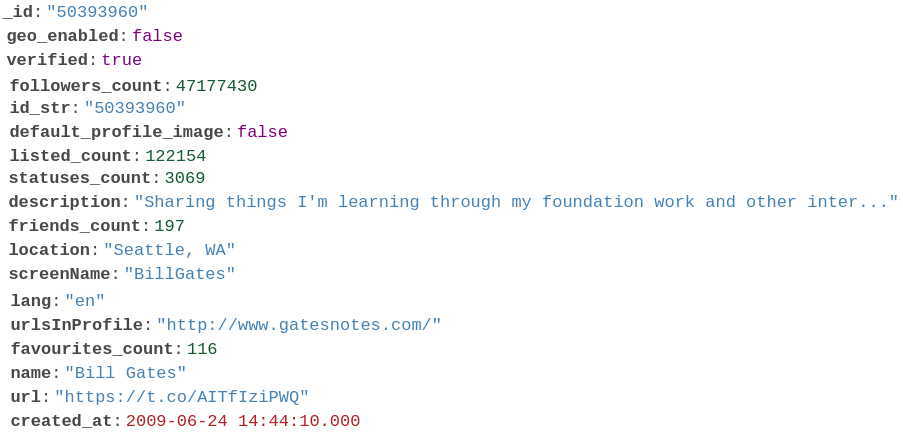
\includegraphics[width=5in]{Fig3.png}}
\caption{Example fields for Twitter User Object corresponding to @BillGates}
\label{fig_ch7_3}
\end{figure}

\item User Object to Demographics: User's textual location is matched against GeoNames city/country pairs, the self-reported name is matched against names with known gender and ethnicity. The associated demographic info, for all followers and all influencers, is stored in tables `userInfoDemographics' and `followerInfoDemographics', respectively. If gender is present it is given by `pctFemale' and `pctMale'; race given by `pctapi': Asian, `pctblack': African American, `pctwhite': Caucasian, `pcthispanic': Hispanic. %For example, for \emph{@kobebryant} the name Kobe is 96.87\% male and the last name Bryant is 58.46\% Caucasian and 35.58\% African American. The details for how these are computed are given later on.

\item Demographics to Distributions: all influencer's followers with gender, race, location, language, time information are used to form corresponding frequency distributions. These distributions can then be used to understand the influencer's influence over the ordinary population by analyzing the percent of influencer's followers within certain gender, language, and so on. %These distributions are stored in DB: `twitter{\_}demographics{\_}across{\_}followers'. 
%As an example the top ten influencers out of 3104 influencers with over 50.0\% of their followers speaking the Turkish language shown in Fig \ref{fig_ch7_4}.
\end{itemize}

\iffalse
\begin{figure}[htbp]
\centerline{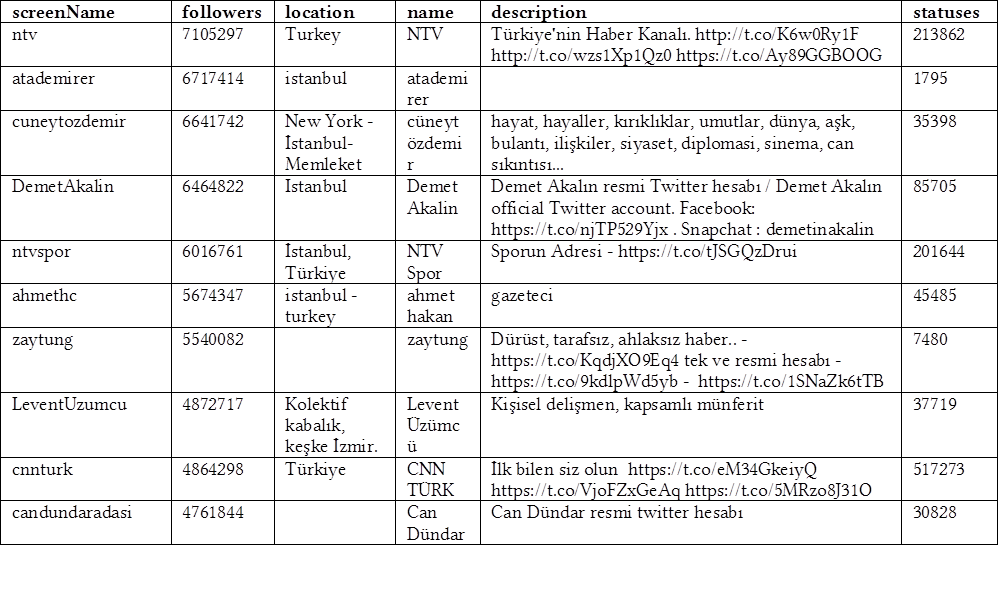
\includegraphics[width=5.4in]{Fig7.png}}
\caption[Top influencers of Turkish speakers]{Top 10 Influencers with mostly Turkish speaking audience.}
\label{fig_ch7_4}
\end{figure}
\fi

ElasticSearch is utilized for loading and exploring data that is relevant to a specific scenario. Thus while MongoDB holds all of the data, ElasticSearch is used to search for a specific demographic. The end-user can utilize the Kibana visualization to form custom queries and zoom in and out on the map. Fig. \ref{fig_ch7_5} shows the visualization dashboard over followers for influencer @CNNEE (CNN Espanol) (similarly any one of the 320K influencers can be visualized).

\begin{figure}[htbp]
\centerline{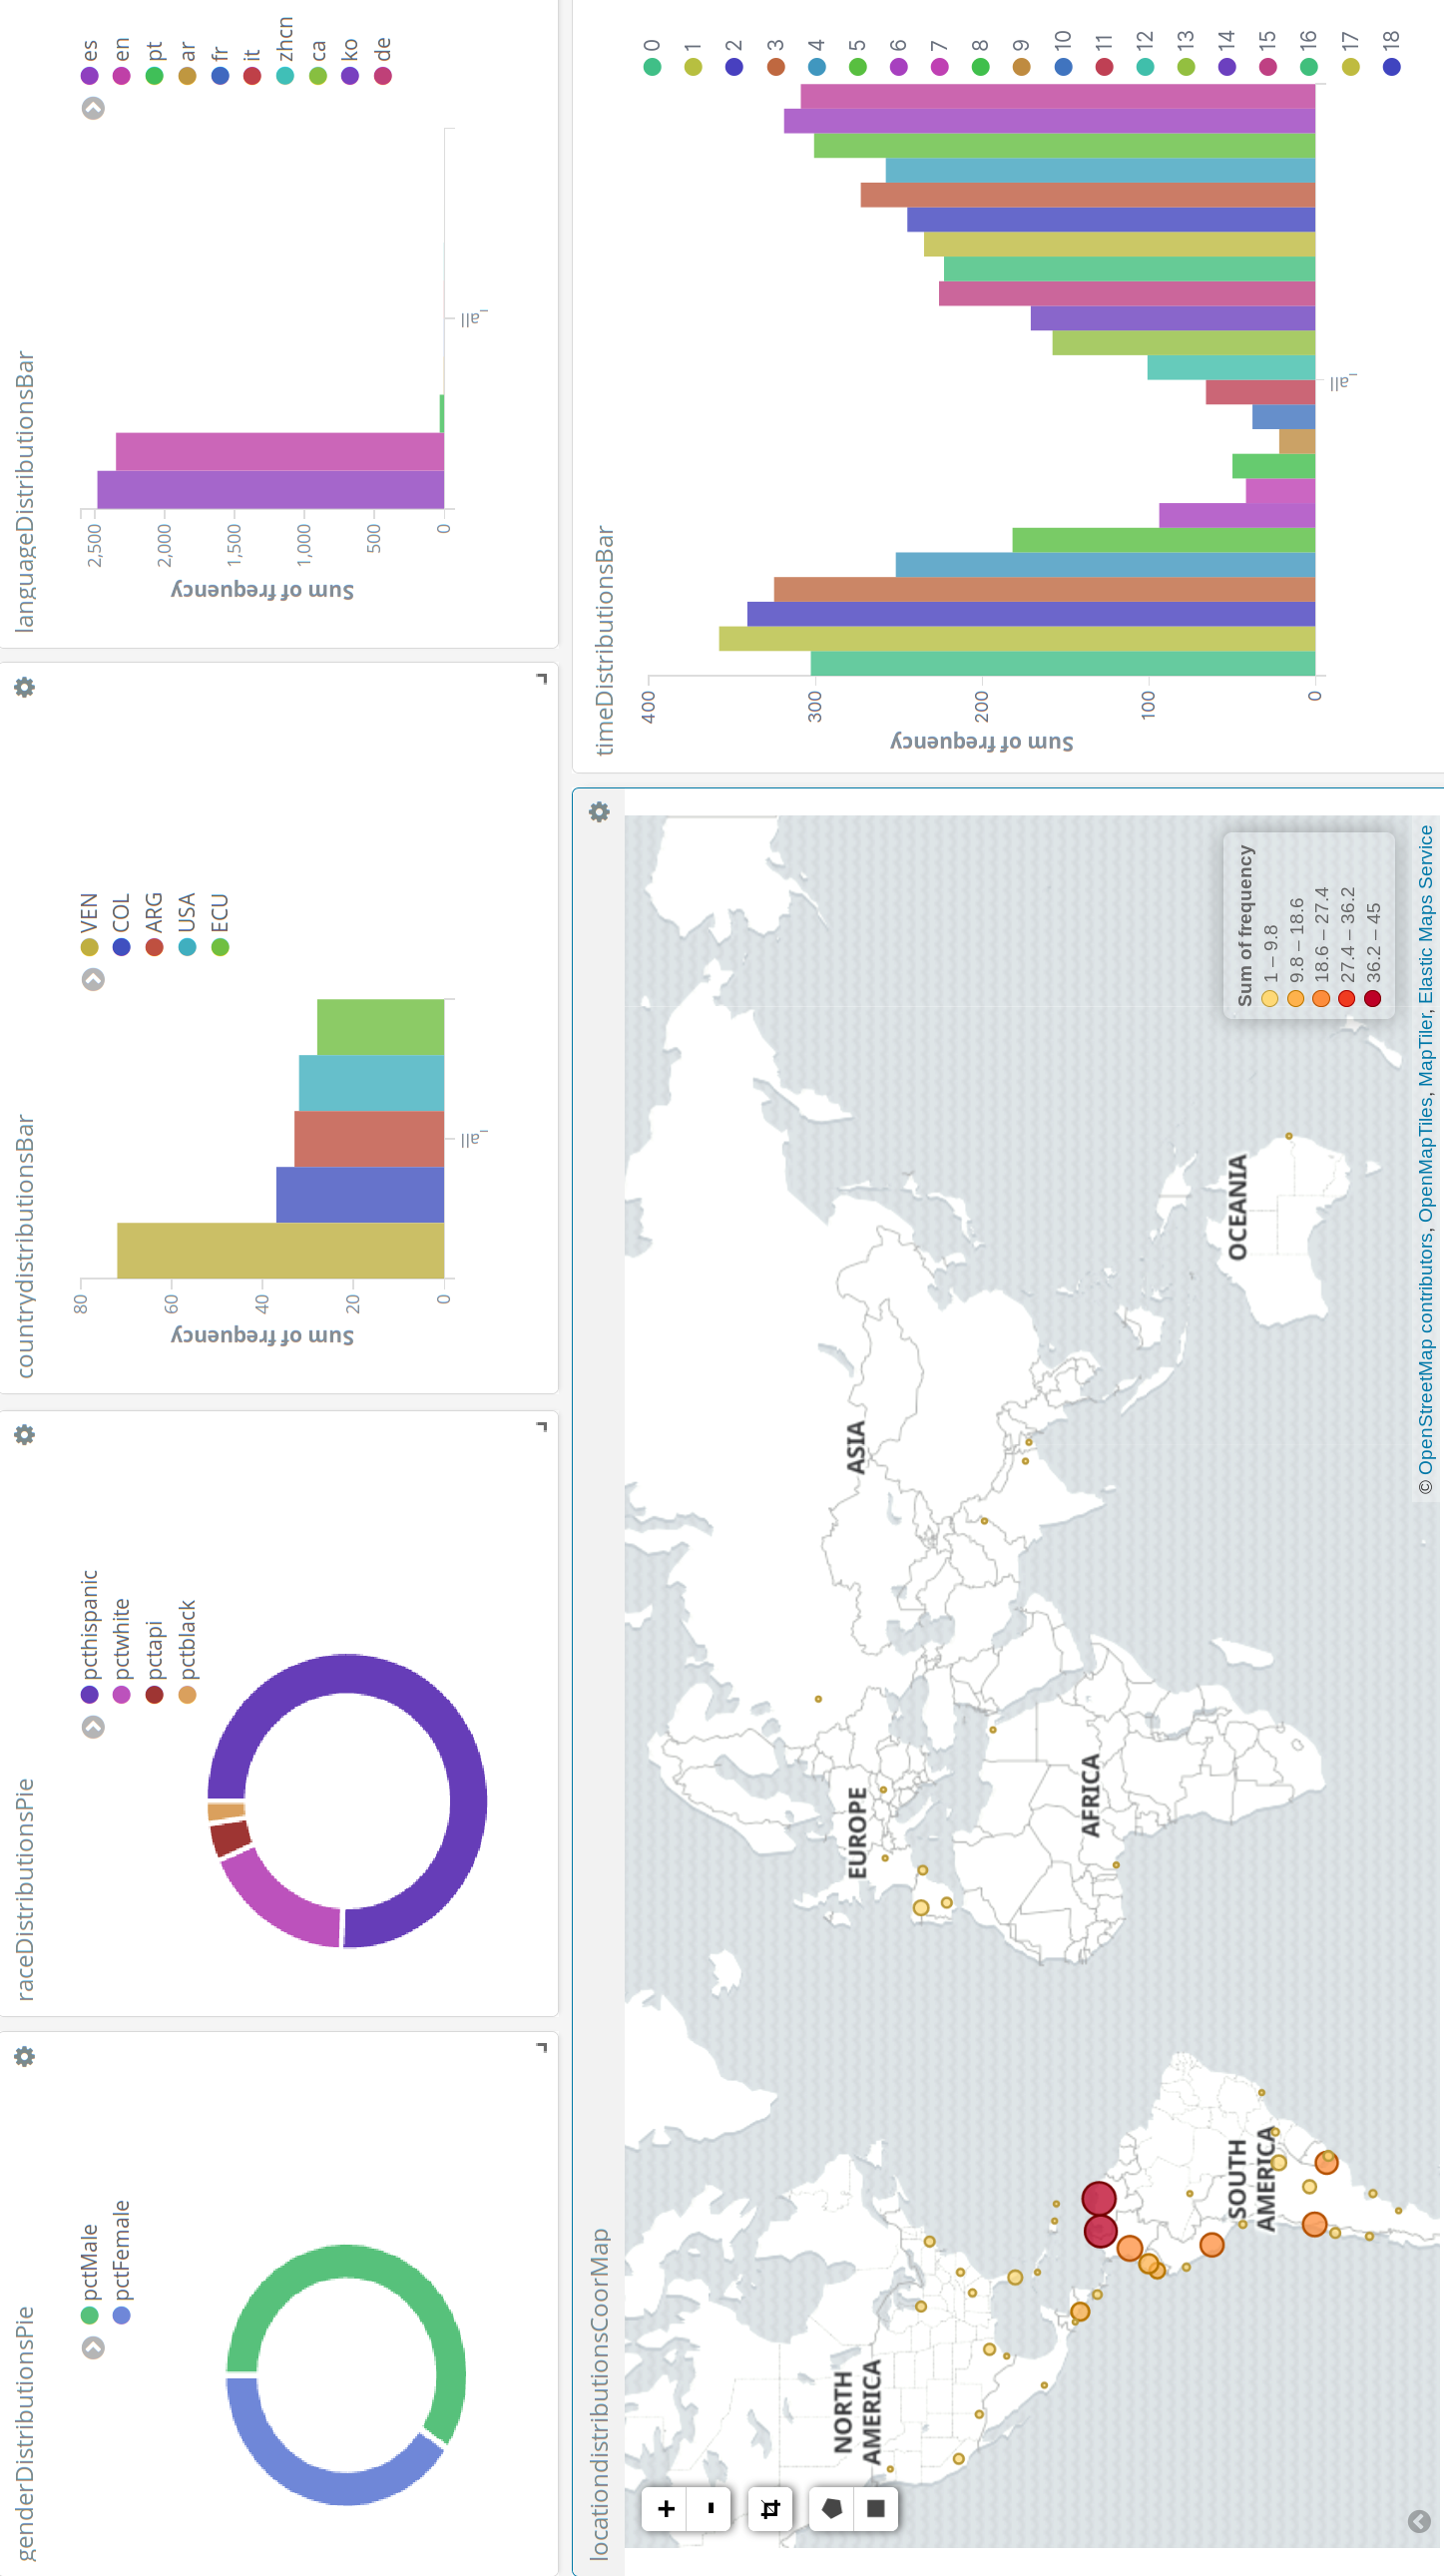
\includegraphics[width=4in]{Fig10.png}}
\caption[Visualizing influence by demographic]{Visualizing influence by demographic. Understanding the influence of @CNNEE.}
\label{fig_ch7_5}
\end{figure}

\section{Features used in Repository}
\subsection{Location}
Chapter 2 described an approach for geocoding a user's textual location. The rules of the classifier developed illustrated that it is important to consider whether a location that is matched contains both the city and state as this is less ambiguous than a city name by itself. Because Google's geocoder is limited, by the number of API calls it can freely make daily, we focused on matching locations that contain a known city/state or city/country for a high precision/low recall solution. For our task, it is better to focus on high precision locations given that verified influencers typically have thousands of followers which generally provides a large enough sample (as seen in section 4.7.2) to accurately pinpoint the influencer's city location.

%Utilizing cities from GeoNames with a population over five thousand\footnote{http://download.geonames.org/export/dump/cities5000.zip}. Country info such as iso codes, fips codes, languages, capital, are also collected from GeoNames\footnote{http://download.geonames.org/export/dump/countryInfo.txt}. 
GeoNames data is processed by (i) verifying each city entry to have a population above five thousand (806 entries were filtered out) and (ii) removing duplicate entries that refer to the same city by taking the most recent entry or one with the highest population (981 entries removed).

\begin{table}
\small
\caption{Countries with most and least cities from GeoNames}
\label{table_1_app2}
\begin{center}
\begin{tabular}{|c|c|c|c|}
\multicolumn{2}{c}{\bfseries Top 20 Country to City} &
\multicolumn{2}{c}{\bfseries Bottom 20 Country to City}\\
\hline
United States & 7113 & Saint Martin & 1 \\
\hline
India & 3189 & Sao Tome and Principe & 1 \\
\hline
Germany & 2780 & Guernsey & 1 \\
\hline
Russia & 2525 & Saint Kitts and Nevis & 1 \\
\hline
France & 1972 & Saint Barthelemy & 1 \\
\hline
Italy & 1919 & Saint Pierre and Miquelon & 1 \\
\hline
Brazil & 1854 & Jersey & 1 \\
\hline
Mexico & 1725 & Seychelles & 1 \\
\hline
United Kingdom & 1603 & Cook Islands & 1 \\
\hline
Spain & 1302 & Tonga & 1 \\
\hline
Philippines & 1160 & British Virgin Islands & 1 \\
\hline
China & 842 & Gibraltar & 1 \\
\hline
Australia & 816 & Palau & 1 \\
\hline
Romania & 755 & Grenada & 1 \\
\hline
Japan & 739 & Faroe Islands & 1 \\
\hline
Turkey & 714 & Antigua and Barbuda & 1 \\
\hline
Poland & 661 & Dominica & 1 \\
\hline
Ukraine & 641 & Barbados & 1 \\
\hline
Netherlands & 484 & Aland Islands & 1 \\
\hline
Colombia & 484 & Macao & 1 \\
\hline
\end{tabular}
\end{center}
\end{table}

For each city, the City + Country Name, Country ISO, Country FIPS, and Country ISO3 are recorded as query strings. For example, for London UK these are the possible strings: `londongbr', `londonuk', `londonunitedkingdom', `londongb'. For the United States, we also search for City + State Name or State Abbreviation; for example `uticany', `uticanewyork'. The country name is utilized for cities with a population over 100K: `syracuseunitedstates', `syracuseus', `syracuseusa' (fips and iso equal in this example). This is done for cities where there is no other city with population over 100K (example `arlingtonus' is not allowed since it can refer to Arlington TX or Arlington VA which both have a population over 100K). There are also cities such as New York City which have `City' as part of the name, but that users may choose not to spell out; we allow city name variations with following tokens removed: `municipality', `village', `city', `charter', `township', and `town'. %So for New York NY USA the possibilities are: newyorkusa, newyorkcityny (with and without `city'). Thus in our representation there are a total of ten string representations for New York NY USA: newyorkusa, newyorkcityunitedstates, newyorkcityus, newyorkcitynewyork, newyorkcityny, newyorkcityusa, newyorkny, newyorkus, newyorknewyork, and newyorkunitedstates. 

In all, there were 47119 unique cities and 156037 corresponding representations. Each follower's self-reported location is turned to lowercase with punctuation and whitespace stripped out. Follower's preprocessed location is utilized if it matches one of the 156037 corresponding representations. Table \ref{table_1_app2} shows the number of unique cities associated with each country. 

In all 225 countries are represented. For each influencer, locations over all followers are used to form a location distribution. The cities in location distribution can be aggregated to generate a country distribution. Location and country distributions are used to identify influencers serving a specific region of the world.

\subsection{Gender}
Social Security Administration (SSA) provides popular female and male names\footnote{https://www.ssa.gov/oact/babynames/names.zip}. The data contains the name, gender, and frequency. A specific name can be used as a female and a male example from file: Emma, F, 19738 and Emma, M, 14. The frequency for gender divided by total frequency gives a percentage for how likely a particular name is to be male vs. female. Given frequencies for Emma, P(Emma, F) = 99.93\% and P(Emma, M) = 0.071\% as probabilities for female and male, respectively. Some names are on the borderline: Temiloluwa 55\%, Carroll 45.5\%, and Arley 57.3\% (male probability). 

This dataset consisted of 29910 names. For each Twitter follower, the first token of the name field is utilized. The token is converted to lowercase with punctuation stripped out. If it is contained within the names dataset then it is assigned a gender probability. For each influencer, the male and female probabilities over followers are added up and divided by the number of followers with name information.

\subsection{Ethnicity}
The Census Bureau identifies the last name to race mapping. The 2010 dataset provides Surnames Occurring 100 or more times with 162254 surnames\footnote{https://www2.census.gov/topics/genealogy/2010surnames/names.zip}. We use the following four race categories: Non-Hispanic White Alone (White), Non-Hispanic Black or African American Alone (Black), Non-Hispanic Asian and Native Hawaiian and Other Pacific Islander Alone (Asian) and Hispanic or Latino origin (Hispanic) (there are two more categories, but those have too few data points, see reference [\ref{appendix:4.12}]).
%Non-Hispanic White Alone, Non-Hispanic Black or African American Alone, Non-Hispanic American Indian and Alaska Native Alone, Non-Hispanic Asian and Native Hawaiian and Other Pacific Islander Alone, Non-Hispanic Two or More Races, and Hispanic or Latino origin. Method focuses on four categories: Non-Hispanic White Alone (Pctwhite), Non-Hispanic Black or African American Alone (Pctblack), Non-Hispanic Asian and Native Hawaiian and Other Pacific Islander Alone (Pctapi) and Hispanic or Latino origin (Pcthispanic). This is inspired by reference [\ref{appendix:4.12}] where authors also focus on these four categories (other categories such as Alaskan Native have too few data points). 
For each Twitter follower, if the self-reported name contains two tokens then the second token of the name field is utilized. The token is converted to lowercase with punctuation stripped out. If it is contained within the surnames dataset then it is utilized. For each influencer, the ethnicity probabilities over followers are added up and divided by the number of followers with ethnicity information. 

\subsection{Time and Language}

\begin{table}
\small
\caption{Top 20 Languages Across the Dataset}
\label{table_2_app2}
\begin{center}
\begin{tabular}{|c|c|c|}
\hline
\bfseries language code& \bfseries follower count& \bfseries overall percent\\
\hline
en&244313028&64.7\\
\hline
es&33680216&8.92\\
\hline
ja&13899866&3.68\\
\hline
ar&11024275&2.92\\
\hline
pt&10550007&2.79\\
\hline
fr&10374538&2.75\\
\hline
tr&9024648&2.39\\
\hline
ru&7717812&2.04\\
\hline
engb&5279311&1.4\\
\hline
none&4495906&1.19\\
\hline
id&4373498&1.16\\
\hline
de&4154066&1.1\\
\hline
it&3094860&0.82\\
\hline
zhcn&2942235&0.78\\
\hline
nl&1965084&0.52\\
\hline
ko&1340514&0.35\\
\hline
vi&1154730&0.31\\
\hline
pl&959457&0.25\\
\hline
th&933313&0.25\\
\hline
sv&753957&0.2\\
\hline
zhtw&613812&0.16\\
\hline
\end{tabular}
\end{center}
\end{table}

The time distribution over influencer's followers is generated as described in Section 5.2. The language field is available for 98.81\% of users. %On Twitter users specify the language that they would want their Twitter dashboard to display in. 
Table \ref{table_2_app2} shows the top 20 languages over 373116407 users. The table shows that about 64.7\% of users prefer English, 8.92\% prefer Spanish, 3.68\%  prefer Japanese, and so on. %Only 1.19\% of users have no info for this field. 
For each influencer, the ratio of followers preferring a specific language is recorded. Influencers who target a specific country such as Spain are expected to have an above average number of Spanish speakers.

\subsection{DBPedia}

\iffalse
\begin{figure}[htbp]
\centerline{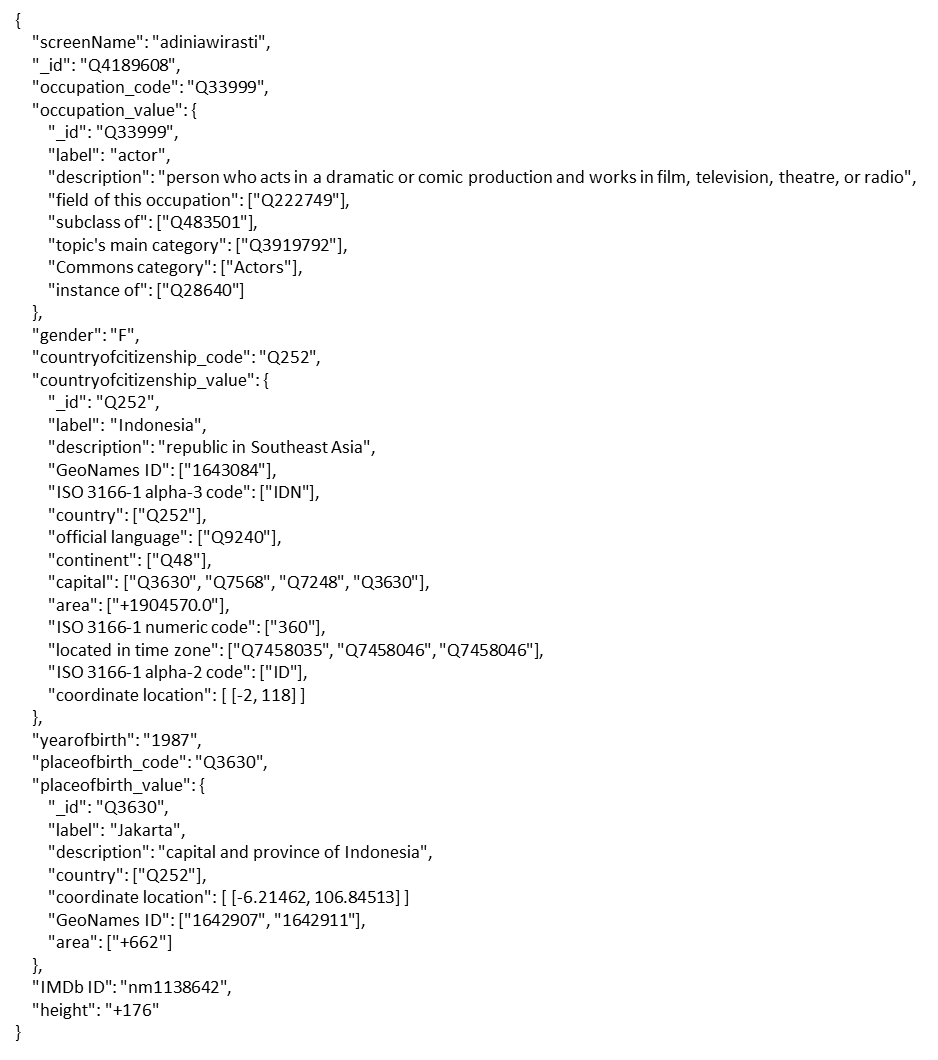
\includegraphics[width=6in]{Fig11.png}}
\caption[DBPedia Data]{Example of additional data brought via DBPedia.}
\label{fig_ch7_6}
\end{figure}
\fi

DBPedia is a large publicly available resource that is used for leveraging external data related to Twitter users. We are interested in those DBPedia pages that have a matching Twitter screenname. Sometimes this will be part of infobox data, other times this data can be predicted. Reference [\ref{appendix:4.15}] is an example of a recent paper that attempts to match DBPedia pages to Twitter screennames. For training and test data, they try the top-ranked Twitter profile (if any) returned by Twitter when queried with the DBPedia entity name. 893,446 DBPedia entities were matched to 630,767 Twitter candidates and a Deep Neural Net (DNN) used to align 169,748 of these. For evaluation, their gold standard is made of those DBpedia pages where the Twitter screenname is explicitly stated consisting of 56,133 alignments from English DBpedia entities (40,967 persons, 15,166 organizations). 

We utilize SocialLink latest Gold and latest predicted mappings that had a score of 0.75 or greater (75\% or higher confidence). Out of these influencers, 44450 appear in our dataset (12,771 from gold and 36,029 from predicted, some influencers appear in both lists).

DBPedia uses a Virtuoso RDF triple store that requires SPARQL queries. If a page exists on Wikipedia such as: `https://en.wikipedia.org/wiki/Oprah{\_}Winfrey' it is also available on DBPedia `http://dbpedia.org/page/Oprah{\_}Winfrey' (unique id being `Oprah{\_}Winfrey'). A Python client library called Wikidata\footnote{https://github.com/dahlia/wikidata} was used.

Each DBPedia page is represented by Q{\#}. Each result contains the label, description, claims, and references. The first step was to collect all claims for each DBPedia page that had a link to a Twitter influencer. The frequency of all unique claims was recorded with some of the items of interest from Table \ref{table_3_app2}. 

\begin{table}
\small
\caption{DBPedia Categories of Interest}
\label{table_3_app2}
\begin{center}
\begin{tabular}{|c|c|c|}
\hline
\bfseries DBPedia ID & \bfseries label & \bfseries Number of Values\\
\hline
P27 & country of citizenship & 224\\
\hline
P569 & date of birth & 9245\\
\hline
P172 & ethnic group & 213\\
\hline
P1412 & languages spoken, written or signed & 141\\
\hline
P21 & sex or gender & 8\\
\hline
P19 & place of birth & 9245\\
\hline
P140 & religion & 124\\
\hline
P69 & educated at & 5660\\
\hline
P735 & given name & 6222\\
\hline
P734 & family name & 10420\\
\hline
P106 & occupation & 1207\\
\hline
P641 & sport & 194\\
\hline
P54 & member of sports team & 5143\\
\hline
P136 & genre & 649\\
\hline
\end{tabular}
\end{center}
\end{table}

Each item listed points to a separate DBPedia page. For example, there are is a separate page for each country, where each page provides additional information such as the country's coordinates, population, inception date, and other information. In this way, for each influencer, we attempt to collect all categories shown in Table \ref{table_3_app2} and then for each category we collect additional information that characterizes the category. This leads to a rich set of additional data available for influencers that are popular enough to be described on Wikipedia. %Fig 5.6 shows a snapshot of brought in data showing an influencer's occupation, place of birth, and country of citizenship. All items marked with QQ{\#} refer to DBPedia pages from which more info can be extracted.

\section{Example Rankings by Demographic Group}

This section illustrates how the repository can be used for content recommendation for a certain demographic; where the demographic is based on gender, ethnicity, language, location, or a combination of these. 

For each demographic feature, our approach is to (i) for each influencer to record the percent of followers that fall into the demographic, (ii) record the average and standard deviation of the percent across all influencers, and (iii) set threshold equal to average plus one standard deviation. Table \ref{table_summaryFeatures_app2} shows the computed thresholds for demographic features related to gender and ethnicity.

\begin{table}
\small
\caption[Demographic Feature Ranges for Gender and Ethnicity]{For each Feature, the Average and Standard Deviation are computed across 320K influencers. This sets a threshold for influencers that capture above the average demographic. Number of influencers recommended for each demographic feature shown in last column.}
\label{table_summaryFeatures_app2}
\begin{center}
\begin{tabular}{|c|c|c|c|c|}
\hline
\bfseries Feature & \bfseries AVG & \bfseries STD & \bfseries T = AVG+STD & \bfseries Influencers\\
\hline
Gender Male & 61.69\% & 16.37\% & 78.06\% & 61988 \\
\hline
Gender Female & 38.34\% & 16.35\% & 54.69\% & 46935 \\
\hline
Ethnicity White & 60.39\% & 17.89\% & 78.28\% & 19179 \\
\hline
Ethnicity Black & 10.95\% & 5.09\% & 16.04\% & 26256 \\
\hline
Ethnicity Hispanic & 13.65\% & 16.26\% & 29.92\% & 33010 \\
\hline
Ethnicity Asian & 11.72\% & 15.03\% & 26.75\% & 33300 \\
\hline
\end{tabular}
\end{center}
\end{table}

\begin{table}
\small
\caption[Top Influencers with male vs. female audience]{Top 10 Most Popular Influencers for each Gender.}
\label{table_4_app2}
\begin{center}
\begin{tabular}{|c|c|c|c|}
\multicolumn{4}{c}{\bfseries Top 10 Influencers with over 78.06\% Followers being male}\\
\hline
\bfseries screenName & \bfseries followers & \bfseries name & \bfseries {\%}Male\\
\hline
narendramodi & 47235007 &Chowkidar Narendra Modi& 81.39 \\
\hline
SrBachchan & 37091473 &Amitabh Bachchan& 80.41\\
\hline
BeingSalmanKhan & 36816795 & Salman Khan & 81.18\\
\hline
SportsCenter & 35437313 & SportsCenter & 78.58\\
\hline
realmadrid & 31984155 & Real Madrid C.F. & 85.34\\
\hline
akshaykumar & 30511248 & Akshay Kumar  & 78.97\\
\hline
FCBarcelona & 29627195 & FC Barcelona & 85.0\\
\hline
imVkohli & 29436203 & Virat Kohli & 83.95\\
\hline
sachin{\_}rt & 29057313 & Sachin Tendulkar & 84.32\\
\hline
PMOIndia & 28895265 & PMO India & 83.17\\
\hline
\multicolumn{4}{c}{}\\
\multicolumn{4}{c}{\bfseries Top 10 Influencers with over 54.69\% Followers being female}\\
\hline
\bfseries screenName & \bfseries followers & \bfseries name & \bfseries{\%}Female\\
\hline
justinbieber & 105481835 & Justin Bieber & 64.03\\
\hline
TheEllenShow & 77630706 & Ellen DeGeneres &62.09\\
\hline
ArianaGrande & 62676030 & Ariana Grande & 59.2\\
\hline
KimKardashian & 60662411 &Kim Kardashian West& 57.68\\
\hline
selenagomez & 57579185 & Selena Gomez & 58.51\\
\hline
jimmyfallon & 51109039& jimmy fallon & 55.94\\
\hline
MileyCyrus & 42505219 & Miley Ray Cyrus & 58.68\\
\hline
NiallOfficial & 39292796 & Niall Horan & 62.67\\
\hline
Harry{\_}Styles & 33315825 & Harry Styles. & 79.25\\
\hline
Louis{\_}Tomlinson & 33232768 & Louis Tomlinson & 67.75\\
\hline
\end{tabular}
\end{center}
\end{table}

\iffalse
\begin{table}
\small
\caption[Top Influencers with male vs. female audience]{Top 10 Most Popular Influencers for each Gender.}
\label{table_4_app2}
\begin{center}
\begin{tabular}{|c|c|c|c|c|}
\multicolumn{5}{c}{\bfseries Top 10 Influencers with over 78.06\% Followers being male}\\
\hline
\bfseries screenName & \bfseries followers & \bfseries profile location & \bfseries name & \bfseries {\%}Male\\
\hline
narendramodi & 47235007 & India &Chowkidar Narendra Modi& 81.39 \\
\hline
SrBachchan & 37091473 & Mumbai, India &Amitabh Bachchan& 80.41\\
\hline
BeingSalmanKhan & 36816795 & MUMBAI & Salman Khan & 81.18\\
\hline
SportsCenter & 35437313 &  & SportsCenter & 78.58\\
\hline
realmadrid & 31984155 & Madrid, Spain & Real Madrid C.F. & 85.34\\
\hline
akshaykumar & 30511248 &  & Akshay Kumar  & 78.97\\
\hline
FCBarcelona & 29627195 & Barcelona & FC Barcelona & 85.0\\
\hline
imVkohli & 29436203 &  & Virat Kohli & 83.95\\
\hline
sachin{\_}rt & 29057313 &UT: 18.986431,72.823769& Sachin Tendulkar & 84.32\\
\hline
PMOIndia & 28895265 & India  & PMO India & 83.17\\
\hline
\multicolumn{5}{c}{}\\
\multicolumn{5}{c}{\bfseries Top 10 Influencers with over 54.69\% Followers being female}\\
\hline
\bfseries screenName & \bfseries followers & \bfseries profile location & \bfseries name & \bfseries{\%}Female\\
\hline
justinbieber & 105481835 &  & Justin Bieber & 64.03\\
\hline
TheEllenShow & 77630706 & California & Ellen DeGeneres &62.09\\
\hline
ArianaGrande & 62676030 & honeymoon ave & Ariana Grande & 59.2\\
\hline
KimKardashian & 60662411 &   &Kim Kardashian West& 57.68\\
\hline
selenagomez & 57579185 & Los Angeles & Selena Gomez & 58.51\\
\hline
jimmyfallon & 51109039 &New York,New York& jimmy fallon & 55.94\\
\hline
MileyCyrus & 42505219 &  & Miley Ray Cyrus & 58.68\\
\hline
NiallOfficial & 39292796 &Mullingar,Westmeath,Ireland& Niall Horan & 62.67\\
\hline
Harry{\_}Styles & 33315825 &  & Harry Styles. & 79.25\\
\hline
Louis{\_}Tomlinson & 33232768 & Doncaster & Louis Tomlinson & 67.75\\
\hline
\end{tabular}
\end{center}
\end{table}
\fi

\noindent\textbf{Gender}-- The gender was computed for 185078761 out of 373116407 (49.6\%) of users. Across all users 57.6\% were male. Across all influencers on average 61.69\% of followers were male with a standard deviation of 16.37\% (threshold = 61.69\%+16.37\% = 78.07\%). The last column shows that there were 61988 influencers whose audience is over 78.07\% male. Top ten influencers exceeding this threshold and ordered by the number of followers shown in Table \ref{table_4_app2} (top). Similarly, 46935 influencers whose audience is over 54.69\% female, with the corresponding top ten influencers shown in Table \ref{table_4_app2} (bottom). 

\noindent\textbf{Ethnicity}-- For ethnicity, 125780191 out of 373116407 (33.71\%) users had, as a second token in their name, a surname that maps to a known ethnicity. Of these 56.54\% were White, 18.21\% Hispanic, 13.98\% Asian, and 10.27\% Black. Table \ref{table_summaryFeatures_app2} shows the computed thresholds for each ethnicity across influencers' followers. Using these thresholds the top influencers for each ethnicity shown in Table \ref{table_6_app2}. %Note: Hindus are not broken out as a separate ethnicity and as a result are associated with Asians (India falls into South Asia), for this reason some influencers with Asian audience are from India.

\begin{table}
\small
\caption[Top Influencers for each Ethnicity]{Most Popular Influencers for each Ethnicity.}
\label{table_6_app2}
\begin{center}
\begin{tabular}{|c|c|c|c|}
\multicolumn{4}{c}{\bfseries Top 6 Influencers with over 78.28\% Followers being Caucasian}\\
\hline
\bfseries screenName & \bfseries followers & \bfseries name & \bfseries {\%}Caucasian\\
\hline
lorenzojova & 3819516 & Lorenzo Jovanotti & 79.13 \\
\hline
repubblica & 2857050 & la Repubblica & 78.6 \\
\hline
SPIEGELONLINE & 2529707 & SPIEGEL ONLINE & 78.76 \\
\hline
beppe{\_}grillo & 2470978 & Beppe Grillo & 79.78 \\
\hline
MarroneEmma & 2469369 & Emma Marrone & 80.44 \\
\hline
radiodeejay & 2278769 & Radio Deejay & 81.63 \\
%\hline
%officiallyjoko & 2204608 & joko winterscheidt & 82.17 \\
%\hline
%redazioneiene & 2199359 & Le Iene & 81.82 \\
%\hline
%ligabue & 2177024 & Luciano Ligabue & 81.38 \\
%\hline
%m{\_}hunziker & 2168051 & Michelle Hunziker & 79.52 \\
\hline
\multicolumn{4}{c}{}\\
\multicolumn{4}{c}{\bfseries Top 6 Influencers with over 16.04\% Followers being African American}\\
\hline
\bfseries screenName & \bfseries followers & \bfseries name & \bfseries {\%}Black\\
\hline
Oprah & 42164712 & Oprah Winfrey & 16.51 \\
\hline
KevinHart4real & 35194359 & Kevin Hart & 16.12 \\
\hline
LilTunechi & 34235040 & Lil Wayne WEEZY F & 19.82 \\
\hline
wizkhalifa & 34028999 & Wiz Khalifa & 16.51 \\
\hline
chrisbrown & 30245761 & Chris Brown & 19.24 \\
\hline
aliciakeys & 30023640 & Alicia Keys & 18.01 \\
%\hline
%andresiniesta8 & 24127051 & Andrés Iniesta & 16.52 \\
%\hline
%MesutOzil1088 & 24016907 & Mesut Özil & 18.18 \\
%\hline
%NICKIMINAJ & 20455827 & QUEEN & 17.63 \\
%\hline
%premierleague & 19432386 & Premier League & 18.75 \\
\hline
\multicolumn{4}{c}{}\\
\multicolumn{4}{c}{\bfseries Top 6 Influencers with over 29.92\% Followers being Hispanic}\\
\hline
\bfseries screenName & \bfseries followers & \bfseries name & \bfseries {\%}Hispanic\\
\hline
shakira & 51127526 & Shakira & 35.82 \\
\hline
Louis{\_}Tomlinson & 33232768 & Louis Tomlinson & 33.29 \\
\hline
realmadrid & 31984155 & Real Madrid C.F. & 31.11 \\
\hline
pitbull & 26128582 & Pitbull & 31.71 \\
\hline
ricky{\_}martin & 20383994 & Ricky Martin & 56.29 \\
\hline
AlejandroSanz & 19516691 & Alejandro Sanz & 71.78 \\
%\hline
%3gerardpique & 19243546 & Gerard Piqué & 40.37 \\
%\hline
%10Ronaldinho & 18624086 & Ronaldinho Gaúcho & 31.81 \\
%\hline
%jamesdrodriguez & 18181928 & James Rodríguez & 55.84 \\
%\hline
%DaniloGentili & 17316619 & Danilo Gentili & 32.13 \\
\hline
\multicolumn{4}{c}{}\\
\multicolumn{4}{c}{\bfseries Top 6 Influencers with over 26.75\% Followers being Asian}\\
\hline
\bfseries screenName & \bfseries followers & \bfseries name & \bfseries {\%}Asian\\
\hline
narendramodi & 47235007 & Chowkidar Narendra Modi & 78.17 \\
\hline
BillGates & 47177430 & Bill Gates & 33.24 \\
\hline
iamsrk & 38104866 & Shah Rukh Khan & 73.74 \\
\hline
SrBachchan & 37091473 &Amitabh Bachchan& 76.75 \\
\hline
BeingSalmanKhan & 36816795 & Salman Khan & 72.79 \\
\hline
akshaykumar & 30511248 & Akshay Kumar & 73.73 \\
\hline
%imVkohli & 29436203 & Virat Kohli & 75.84 \\
%\hline
%sachin{\_}rt & 29057313 & Sachin Tendulkar & 76.86 \\
%\hline
%PMOIndia & 28895265 & PMO India & 80.59 \\
%\hline
%deepikapadukone & 26090675 & Deepika Padukone & 75.99 \\
%\hline
\end{tabular}
\end{center}
\end{table}

\iffalse
\begin{table}
\scriptsize
\caption[Top Influencers of different ethnicity]{Top 10 Most Popular Influencers for each Ethnicity.}
\label{table_6_app2}
\begin{center}
\begin{tabular}{|c|c|c|c|c|}
\multicolumn{5}{c}{\bfseries Top 10 Influencers with over 78.28\% Followers being Caucasian}\\
\hline
\bfseries screenName & \bfseries followers & \bfseries profile location & \bfseries name & \bfseries {\%}Caucasian\\
\hline
lorenzojova & 3819516 &  & Lorenzo Jovanotti & 79.13 \\
\hline
repubblica & 2857050 & Rome, Italy & la Repubblica & 78.6 \\
\hline
SPIEGELONLINE & 2529707 & Hamburg, Germany & SPIEGEL ONLINE & 78.76 \\
\hline
beppe{\_}grillo & 2470978 & Genova, Italia & Beppe Grillo & 79.78 \\
\hline
MarroneEmma & 2469369 &  & Emma Marrone & 80.44 \\
\hline
radiodeejay & 2278769 & Italy & Radio Deejay & 81.63 \\
\hline
officiallyjoko & 2204608 & berlin...city & joko winterscheidt & 82.17 \\
\hline
redazioneiene & 2199359 & Milano & Le Iene & 81.82 \\
\hline
ligabue & 2177024 & Correggio (RE) & Luciano Ligabue & 81.38 \\
\hline
m{\_}hunziker & 2168051 & Italy & Michelle Hunziker & 79.52 \\
\hline
\multicolumn{5}{c}{}\\
\multicolumn{5}{c}{\bfseries Top 10 Influencers with over 16.04\% Followers being African American}\\
\hline
\bfseries screenName & \bfseries followers & \bfseries profile location & \bfseries name & \bfseries {\%}Black\\
\hline
Oprah & 42164712 &  & Oprah Winfrey & 16.51 \\
\hline
KevinHart4real & 35194359 & Philly/LA & Kevin Hart & 16.12 \\
\hline
LilTunechi & 34235040 &  & Lil Wayne WEEZY F & 19.82 \\
\hline
wizkhalifa & 34028999 & Pix Burgh & Wiz Khalifa & 16.51 \\
\hline
chrisbrown & 30245761 &  & Chris Brown & 19.24 \\
\hline
aliciakeys & 30023640 & New York City & Alicia Keys & 18.01 \\
\hline
andresiniesta8 & 24127051 & Barcelona & Andrés Iniesta & 16.52 \\
\hline
MesutOzil1088 & 24016907 & England & Mesut Özil & 18.18 \\
\hline
NICKIMINAJ & 20455827 & Q U E E N & QUEEN & 17.63 \\
\hline
premierleague & 19432386 &  & Premier League & 18.75 \\
\hline
\multicolumn{5}{c}{}\\
\multicolumn{5}{c}{\bfseries Top 10 Influencers with over 29.92\% Followers being Hispanic}\\
\hline
\bfseries screenName & \bfseries followers & \bfseries profile location & \bfseries name & \bfseries {\%}Hispanic\\
\hline
shakira & 51127526 & Barranquilla & Shakira & 35.82 \\
\hline
Louis{\_}Tomlinson & 33232768 & Doncaster & Louis Tomlinson & 33.29 \\
\hline
realmadrid & 31984155 & Madrid, Spain & Real Madrid C.F. & 31.11 \\
\hline
pitbull & 26128582 & Miami, FL & Pitbull & 31.71 \\
\hline
ricky{\_}martin & 20383994 & Puerto Rico & Ricky Martin & 56.29 \\
\hline
AlejandroSanz & 19516691 &  & Alejandro Sanz & 71.78 \\
\hline
3gerardpique & 19243546 & Barcelona & Gerard Piqué & 40.37 \\
\hline
10Ronaldinho & 18624086 & Rio de Janeiro, Brasil & Ronaldinho Gaúcho & 31.81 \\
\hline
jamesdrodriguez & 18181928 & Munich, Baviera & James Rodríguez & 55.84 \\
\hline
DaniloGentili & 17316619 & Santo André & Danilo Gentili & 32.13 \\
\hline
\multicolumn{5}{c}{}\\
\multicolumn{5}{c}{\bfseries Top 10 Influencers with over 26.75\% Followers being Asian}\\
\hline
\bfseries screenName & \bfseries followers & \bfseries profile location & \bfseries name & \bfseries {\%}Asian\\
\hline
narendramodi & 47235007 & India & Chowkidar Narendra Modi & 78.17 \\
\hline
BillGates & 47177430 & Seattle, WA & Bill Gates & 33.24 \\
\hline
iamsrk & 38104866 &  & Shah Rukh Khan & 73.74 \\
\hline
SrBachchan & 37091473 & Mumbai, India &Amitabh Bachchan& 76.75 \\
\hline
BeingSalmanKhan & 36816795 & MUMBAI & Salman Khan & 72.79 \\
\hline
akshaykumar & 30511248 &  & Akshay Kumar & 73.73 \\
\hline
imVkohli & 29436203 &  & Virat Kohli & 75.84 \\
\hline
sachin{\_}rt & 29057313 & ÜT: 18.986431,72.823769 & Sachin Tendulkar & 76.86 \\
\hline
PMOIndia & 28895265 & India  & PMO India & 80.59 \\
\hline
deepikapadukone & 26090675 &  & Deepika Padukone & 75.99 \\
\hline
\end{tabular}
\end{center}
\end{table}
\fi

\noindent\textbf{Location}-- There are over 200 countries. For each influencer, the country distribution is formed from self-reported locations of the followers that mention city and country. There are a total of 36980202 out of 373116407 (9.91\%) followers listing such well-formed locations. The known countries are used to generate a distribution that can be used to focus on specific influencers. As an example, Table \ref{table_10_app2} (top) shows the top ten influencers associated with Indonesia (in repository 1663 influencers had over 50.0\% of their followers from Indonesia).

\noindent\textbf{Language}-- Language information is available for over 98.8\% of followers and is thus a powerful feature since there is a large sample size of followers with the field. Table \ref{table_10_app2} (bottom) shows the top ten influencers whose followers are 50\% or more Spanish. The location and description fields of these influencers match Latin America, Mexico, Spain - locations with mostly Spanish speaking audiences. There were 22067 influencers with over 50.0\% of their followers preferring Spanish.

\begin{table}
\small
\caption[Top Influencers of Indonesia (top), speaking Spanish (bottom)]{Top 10 Influencers from Indonesia (top), speaking Spanish (bottom)}
\label{table_10_app2}
\begin{center}
\begin{tabular}{|c|c|c|c|}
\multicolumn{4}{c}{\bfseries Top 10 Influencers with over 50\% Followers from Indonesia}\\
\hline
\bfseries screenName & \bfseries followers & \bfseries profile location & \bfseries {\%}IND\\
\hline
agnezmo & 17649171 & Los Angeles & 91.41 \\
\hline
radityadika & 15734925 & Jakarta Selatan, DKI Jakarta& 97.6 \\
\hline
detikcom & 15102845 & Jakarta, Indonesia & 95.31 \\
\hline
LunaMaya26 & 11651186 & INDONESIA & 94.23 \\
\hline
cinema21 & 11444672 & Jakarta, Indonesia & 94.94 \\
\hline
jokowi & 11384071 & Jakarta & 93.13 \\
\hline
sherinasinna & 10781243 &  & 92.03 \\
\hline
Metro{\_}TV & 10395864 & UT:-6.186977, 106.759125 & 93.43 \\
\hline
SBYudhoyono & 10086130 &  & 95.0 \\
\hline
afgansyah{\_}reza & 9926114 & Indonesia & 94.47 \\
\hline
\multicolumn{4}{c}{}\\
\multicolumn{4}{c}{\bfseries Top 10 Influencers with over 50\% Spanish Followers}\\
\hline
\bfseries screenName & \bfseries followers & \bfseries profile location & \bfseries {\%}Spanish\\
\hline
CNNEE & 17232226 & En todas partes & 50.74 \\
\hline
TwitterLatAm & 14948461 & América Latina & 54.1 \\
\hline
juanes & 11599148 &  & 52.2 \\
\hline
PaulinaRubio & 11209842 &  & 50.29 \\
\hline
CHAYANNEMUSIC & 9290096 & Miami, Florida & 54.63 \\
\hline
SofiaVergara & 8990538 &  & 51.63 \\
\hline
muyinteresante & 8368847 & Spain & 65.47 \\
\hline
werevertumorro & 8330870 & México, DF & 58.89 \\
\hline
AristeguiOnline & 8275955 & México, DF & 60.07 \\
\hline
CarlosLoret & 8033311 & México, DF. & 56.09 \\
\hline
\end{tabular}
\end{center}
\end{table}

\iffalse
\begin{table} \renewcommand{\arraystretch}{0.99}
\scriptsize
\caption[Top Influencers of Indonesia (top), speaking Spanish (bottom)]{Top 10 Influencers from Indonesia (top), speaking Spanish (bottom)}
\label{table_10_app2}
\begin{center}
\begin{tabular}{|c|c|c|c|c|c|}
\multicolumn{5}{c}{\bfseries Top 10 Influencers with over 50\% Followers from Indonesia}\\
\hline
\bfseries screenName & \bfseries followers & \bfseries profile location & \bfseries name & \bfseries {\%}IND\\
\hline
agnezmo & 17649171 & Los Angeles & AGNEZ MO & 91.41 \\
\hline
radityadika & 15734925 & Jakarta Selatan, DKI Jakarta & raditya dika & 97.6 \\
\hline
detikcom & 15102845 & Jakarta, Indonesia & detikcom & 95.31 \\
\hline
LunaMaya26 & 11651186 & INDONESIA & luna maya & 94.23 \\
\hline
cinema21 & 11444672 & Jakarta, Indonesia & Cinema XXI & 94.94 \\
\hline
jokowi & 11384071 & Jakarta & Joko Widodo & 93.13 \\
\hline
sherinasinna & 10781243 &  & Sinna Sherina Munaf & 92.03 \\
\hline
Metro{\_}TV & 10395864 & UT:-6.186977, 106.759125 & METRO TV & 93.43 \\
\hline
SBYudhoyono & 10086130 &  & S. B. Yudhoyono & 95.0 \\
\hline
afgansyah{\_}reza & 9926114 & Indonesia & Afgan & 94.47 \\
%\hline
%\end{tabular}
%end{center}
%\end{table}

\hline
\multicolumn{5}{c}{}\\
\multicolumn{5}{c}{\bfseries Top 10 Influencers with over 50\% Spanish Followers}\\
\hline

%\begin{table}
%\scriptsize
%\caption[Top Influencers of Spanish speakers]{Top 10 Influencers with over 50\% Spanish Followers}
%\label{table_11_app2}
%\begin{center}
%\begin{tabular}{|c|c|c|c|c|c|}
%\hline
\bfseries screenName & \bfseries followers & \bfseries profile location & \bfseries name & \bfseries {\%}Spanish\\
\hline
CNNEE & 17232226 & En todas partes & CNN en Español & 50.74 \\
\hline
TwitterLatAm & 14948461 & América Latina & Twitter Latin America & 54.1 \\
\hline
juanes & 11599148 &  & JUANES & 52.2 \\
\hline
PaulinaRubio & 11209842 &  & Paulina Rubio & 50.29 \\
\hline
CHAYANNEMUSIC & 9290096 & Miami, Florida & CHAYANNE & 54.63 \\
\hline
SofiaVergara & 8990538 &  & Sofia Vergara & 51.63 \\
\hline
muyinteresante & 8368847 & Spain & MUY Interesante & 65.47 \\
\hline
werevertumorro & 8330870 & México, DF & TIMBERS GABOREVER & 58.89 \\
\hline
AristeguiOnline & 8275955 & México, DF & Aristegui Noticias & 60.07 \\
\hline
CarlosLoret & 8033311 & México, DF. & Carlos Loret de Mola & 56.09 \\
\hline
\end{tabular}
\end{center}
\end{table}
\fi


\begin{table}
\renewcommand{\arraystretch}{0.99}
\small
\caption[Verified vs. Unverified Comparison using Messages and Followers]{Verified vs. Unverified number of messages (top) vs. followers (bottom)}
\label{table_12_app2}
\begin{center}
\begin{tabular}{|l|l|l|l|l|}
\multicolumn{5}{c}{\bfseries Verified vs. Unverified Users number of messages posted}\\
\hline
%      \multicolumn{1}{c}{} &
%\multicolumn{2}{c}{\bfseries Unverified} %&
%\multicolumn{2}{c}{\bfseries Verified}\\
%\hline
\bfseries Range & \bfseries Pct & \bfseries Unverified (avg, std) & \bfseries Pct & \bfseries Verified (avg, std)\\
\hline
[0,0] & 24.627 & (0.0, 0.0) & 0.143 & (0.0, 0.0) \\
\hline
[0,10] & 52.125 & (1.88, 2.63) & 0.668 & (3.58, 3.28) \\
\hline
[10,100] & 20.663 & (36.73, 24.57) & 2.466 & (52.19, 26.43) \\
\hline
[100,1000] & 15.390 & (370.92, 243.46) & 14.997 & (500.69, 260.57) \\
\hline
[1000,10000] & 9.999 & (3412.65, 2293.9) & 47.675 & (4365.28, 2518.2) \\
\hline
[10000,100000] & 2.793 & (24997.56, 17105.79) & 31.976 & (27613.0, 18946.36) \\
\hline
[100000,1000000] & 0.094 & (165696.91, 88231.33) & 2.257 & (193657.95, 124088.35) \\
\hline
[1000000,Inf] & 0.0002 & (1481857.94, 1334891.99) & 0.0394 & (2604262.9, 4528258.8) \\
\hline
[0, Inf] & 100 & (1264.22, 8248.86) & 100 & (16381.72, 109704.1) \\
\hline
\multicolumn{5}{c}{}\\
\multicolumn{5}{c}{\bfseries Verified vs. Unverified Users number of followers}\\
\hline
%      \multicolumn{1}{c}{} &
%\multicolumn{2}{c}{\bfseries %Unverified} &
%\multicolumn{2}{c}{\bfseries Verified}\\
%\hline
\bfseries Range & \bfseries Pct & \bfseries Unverified (avg, std) & \bfseries Pct & \bfseries Verified (avg, std)\\
\hline
[0,0] & 15.815 & (0.0, 0.0) & 0.0012 & (0.0, 0.0)\\
\hline
[0,10] & 55.163 & (2.72, 2.86) & 0.0722 & (8.05, 2.67)\\
\hline
[10,100] & 29.49 & (34.9, 23.94) & 0.729 & (42.23, 27.67)\\
\hline
[100,1000] & 14.903 & (305.88, 205.6) & 7.3415 & (587.87, 250.8)\\
\hline
[1000,10000] & 1.928 & (2409.18, 1767.89) & 41.253 & (4361.78, 2504.94) \\
\hline
[10000,100000] & 0.158 & (24420.97, 17754.61) & 36.922 & (33291.61, 22652.99)\\
\hline
[100000,1000000] & 0.0105 & (218116.84, 151487.27) & 11.663 & (294429.2, 208785.86)\\
\hline
[1000000,Inf] & 0.0003 & (1862548.7, 1183416.8) & 2.057 & (3374510.0, 5580356.3)\\
\hline
[0, Inf] & 100 & (170.97, 4921.16) & 100 & (117889.54, 936335.99) \\
\hline
\end{tabular}
\end{center}
\end{table}

\section{Verified vs. Unverified User Comparison}
In this section, the differences between verified (over 322 thousand users) vs. unverified (over 373 million users) are analyzed. The average number of messages, friends, and followers that a user has are analyzed. In previous chapters, it was claimed that most Twitter users are silent consumers of information. Table \ref{table_12_app2} (top) shows the percent of users that are posting a specific rate defined by the range (min, max) for unverified vs. verified users. From Table about 1/4 (24.63\%) never posted any content, about 1/3 (33.01\%) posted less than 1 message, 1/2 (52.12\%) posted 10 or less, and so on. On average, the verified users post 16381 vs. 1264 messages for unverified users. 

In a similar fashion, the average number of followers for verified vs. unverified users is shown in Table \ref{table_12_app2} (bottom). In section 4.7.2 it was shown that at least 500 followers are needed to get a large enough sample for computing the central geographic location that the influencer serves. Using at least 500 influencers 3.581\% of verified vs. 97.077\% of unverified users are lost (thus a vast majority of verified users pass this threshold). The table shows that verified users have a lot more followers on average 117889 vs. 171 for unverified users.

\begin{figure}[htbp]
\centerline{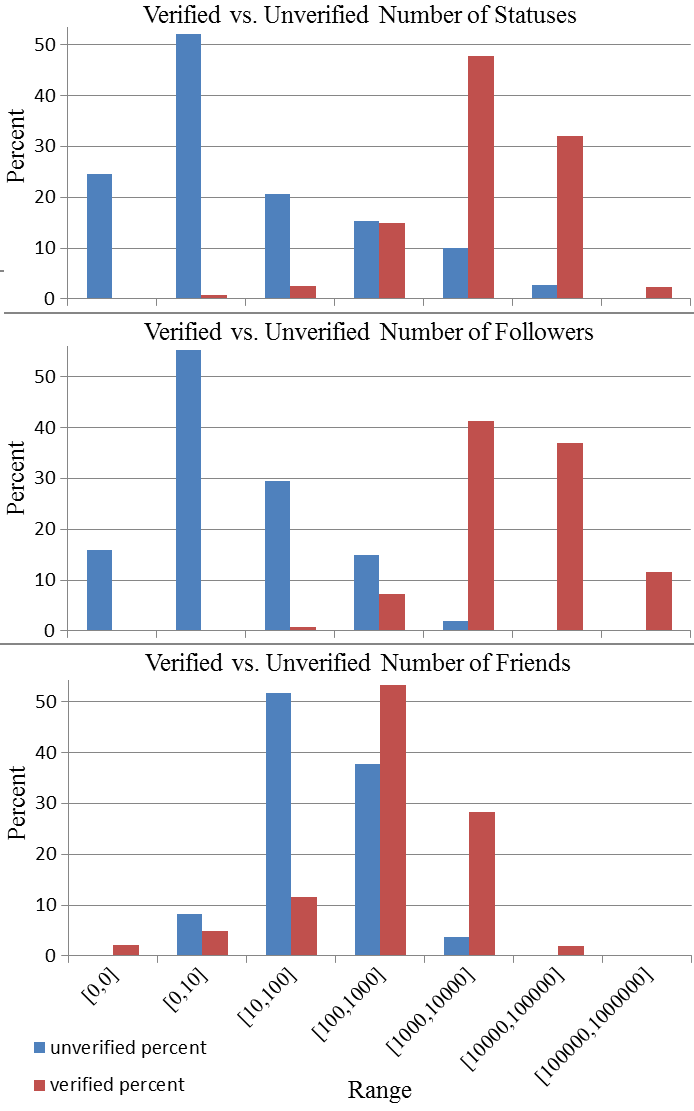
\includegraphics[width=4in]{Fig13.png}}
\caption[Verified vs. Unverified users]{Comparison of Verified vs. Unverified users using: (top) number of messages posted, (middle) total followers, and (bottom) total friends.}
\label{fig_ch7_7}
\end{figure}

Fig. \ref{fig_ch7_7} is a depiction using ranges from Table \ref{table_12_app2} differentiating verified vs. unverified over (i) the total number of messages (top chart), (ii) the total number of followers (middle chart), and (iii) the total number of friends (bottom chart). Fig. \ref{fig_ch7_7} bottom shows that a good portion of verified users is also engaged in following others (forming friend connections).

In summary, verified influencers are more likely to have more messages, more followers, and more friends. Given that most users are passive and do not generate much message traffic supports our argument for focusing on follower-followee link structure and profile metadata for mapping influence.

\section{Conclusions}
The social media site that is Twitter is a big data challenge. Twitter generates 500 million messages on a daily basis. It can be a daunting task to figure out how to collect the information that corresponds to the specific demographic of interest. This chapter presented a tool for quickly identifying influencers serving a specific demographic. This is important for content recommendation where we can identify influencers based on the composition of their audience using gender, ethnicity, language, location, or a combination of these. Also, by focusing on the followers of these influencers a community that is representative of the population of interest can be quickly established.


\chapter{Conclusions}\label{chap:Conclusion}

The main theme of our research is in understanding the geographic spread of a group; where the group can be made up of Twitter users or messages. We have explored (i) location - improving geocoding by customizing an existing geocoder as well as training a high-level geocoder with multilingual support, (ii) time - predicting whether a group is local or global and the associated UTC offset, (iii) inferring location - leverage Twitter network connections to known geo-influencers (users that cater their content to a specific geographic area). 

Google search was leveraged for identifying an initial set of geo-influencers related to a city of interest; it was shown that the geo-influencers' followers are representative of the city's users (i.e. most of the followers are physically located in the city). Location features are necessary for city-level geocoding, but time and language can also help reason about the geographic spread. Research showed that using only time-based features is enough to associate top trending topics and persons with different geographical regions. The new time-based features are not just limited to inferring location, but can also be used for inferring link creation times and for studying the evolution of influencer's popularity.

By maintaining a repository of geo-influencers it is possible to quickly leverage, as a starting point, those influencers within the geographic location of interest vs. having to discover them in a time-intensive collection from scratch (this targetted collection is 100x faster). It was also shown how the repository can be used for filtering influencers based on their audience's demographics related to location, language, gender, and ethnicity.  
This research is important because it enables multiple applications, each of which were shown in our research: (i) content recommendation, (ii) community detection, (iii) inferring the location of users based on the link structure to geo-influencers, and (iv) studying the evolution of influencer's popularity. %Main portions of the code are hosted on GitHub\footnote{https://github.com/apanasyu}.

%For understanding followers' geography, multiple approaches were explored. First using textual locations our research has illustrated how geocoding can be improved by (i) improving Google's geocoder and (ii) via a TF-IDF model that handles foreign languages and is applicable to the Twitter domain. Second through followers time and language features; where the sleep cycle identifies the most probable region of the world and language further limits the set of possible countries (we are not aware of any other research that utilizes the sleep cycle for helping predict a geographic region). Third through link structure; it was illustrated how using an initial set of influencers set A, communities can be established from influencers' followers, and using these communities additional influencers set B can be discovered. 
\begin{thebibliography}{200}
\bibitem{-1}Karami, Amir, et al. "Twitter and research: a systematic literature review through text mining." IEEE Access 8 (2020): 67698-67717.\label{appendix:0.1}
\bibitem{0}Antonakaki, Despoina, Paraskevi Fragopoulou, and Sotiris Ioannidis. "A survey of Twitter research: Data model, graph structure, sentiment analysis and attacks." Expert Systems with Applications 164 (2021): 114006.\label{appendix:0.2}

\bibitem{1}Zheng, Xin, Jialong Han, and Aixin Sun. ``A survey of location prediction on Twitter.`` IEEE Transactions on Knowledge and Data Engineering (2018).\label{appendix:1.1}
\bibitem{2}Graham, Mark, Scott A. Hale, and Devin Gaffney. ``Where in the world are you? Geolocation and language identification in Twitter.`` The Professional Geographer 66.4 (2014): 568-578.\label{appendix:1.2}
\bibitem{3}Mislove, Alan, et al. ``Understanding the Demographics of Twitter Users.`` ICWSM 11.5th (2011): 25.\label{appendix:1.3}
\bibitem{4}Stephens, Monica, and Ate Poorthuis. ``Follow thy neighbor: Connecting the social and the spatial networks on Twitter.`` Computers, Environment and Urban Systems 53 (2015): 87-95.\label{appendix:1.4}
\bibitem{5}Beauchamp, Nicholas. ``Predicting and interpolating state‐level polls using Twitter textual data.`` American Journal of Political Science 61.2 (2017): 490-503.\label{appendix:1.5}
\bibitem{6}Byrd, Kenny, et al. ``Mining Twitter data for influenza detection and surveillance.`` Proceedings of the International Workshop on Software Engineering in Healthcare Systems. ACM, 2016.\label{appendix:1.6}
\bibitem{7}Zubiaga, Arkaitz, et al. ``Towards real-time, country-level location classification of worldwide tweets.`` IEEE Transactions on Knowledge and Data Engineering 29.9 (2017): 2053-2066.\label{appendix:1.7}
\bibitem{8}Jurgens, David, et al. ``Geolocation Prediction in Twitter Using Social Networks: A Critical Analysis and Review of Current Practice.`` ICWSM 15 (2015): 188-197.\label{appendix:1.8}
\bibitem{9}Wong, Charlene A., et al. ``Twitter sentiment predicts Affordable Care Act marketplace enrollment.`` Journal of medical Internet research 17.2 (2015).\label{appendix:1.9}
\bibitem{10}Matci, Dilek Küçük, and Uğur Avdan. ``Address standardization using the natural language process for improving geocoding results.`` Computers, Environment and Urban Systems (2018).\label{appendix:1.10}
\bibitem{11}Jurgens, David. ``That's What Friends Are For: Inferring Location in Online Social Media Platforms Based on Social Relationships.`` ICWSM 13.13 (2013): 273-282.\label{appendix:1.11}
\bibitem{12}Malik, Momin M., et al. ``Population bias in geotagged tweets.`` People 1.3,759.710 (2015): 3-759.\label{appendix:1.12}
\bibitem{13}Tasse, Dan, et al. ``State of the Geotags: Motivations and Recent Changes.`` ICWSM. 2017.\label{appendix:1.13}
\bibitem{14}Prasetyo, Philips., et al. ``On analyzing geotagged tweets for location-based patterns.`` Proceedings of the 17th International Conference on Distributed Computing and Networking. ACM, 2016.\label{appendix:1.14}
\bibitem{15}Laniado, David, et al. ``The Impact of Geographic Distance on Online Social Interactions.`` Information Systems Frontiers(2017): 1-16.\label{appendix:1.15}
\bibitem{16}Singh, Sushant K. ``Evaluating two freely available geocoding tools for geographical inconsistencies and geocoding errors.`` Open Geospatial Data, Software and Standards 2.1 (2017): 11\label{appendix:1.16}
\bibitem{17}Vincenty, Thaddeus. ``Direct and inverse solutions of geodesics on the ellipsoid with application of nested equations.`` Survey review 23.176 (1975): 88-93.\label{appendix:1.17}
\bibitem{18}Miyazaki, Taro, et al. ``Twitter Geolocation using Knowledge-Based Methods.`` Proceedings of the 2018 EMNLP Workshop W-NUT: The 4th Workshop on Noisy User-generated Text. 2018.\label{appendix:1.18}

\bibitem{19}Riquelme, Fabián, and Pablo González-Cantergiani. ``Measuring user influence on Twitter: A survey.`` Information Processing \& Management 52.5 (2016): 949-975.\label{appendix:2.1}
\bibitem{20}Bouros, Panagiotis, Dimitris Sacharidis, and Nikos Bikakis. ``Regionally influential users in location-aware social networks.`` Proceedings of the 22nd ACM SIGSPATIAL International Conference on Advances in Geographic Information Systems. ACM, 2014.\label{appendix:2.2}
\bibitem{21}Li, Guoliang, et al. ``Efficient location-aware influence maximization.`` Proceedings of the 2014 ACM SIGMOD international conference on Management of data. ACM, 2014.\label{appendix:2.3}
\bibitem{22}Darmon, David, Elisa Omodei, and Joshua Garland. ``Followers are not enough: A multifaceted approach to community detection in online social networks.`` PloS one 10.8 (2015): e0134860.\label{appendix:2.4}
\bibitem{23}Java A, Song X, Finin T, Tseng B (2009) Why we twitter: an analysis of a microblogging community. In: Advances in Web Mining and Web Usage Analysis, Springer. pp. 118–138.\label{appendix:2.5}
\bibitem{24}Wang, T.-C.; Phoa, F.K.H.: A scanning method for detecting clustering pattern of both attribute and structure in social networks. Phys. A Stat. Mech. Appl. 445, 295–309 (2016)\label{appendix:2.6}
\bibitem{25}Yang, J.; McAuley, J.; Leskovec, J.: Community detection in networks with node attributes. In: IEEE 13th International Conference on Data mining (ICDM), pp. 1151–1156. IEEE (2013)\label{appendix:2.7}
\bibitem{26}Zhang, F.; Li, J.; Li, F.; Xu, M.; Xu, R.; He, X.: Community detection based on links and node features in social networks. In: He, X., Luo, S., Tao, D., Xu, C., Yang, J., Hasan, M.A. (eds.) MultiMedia Modeling. MMM 2015. Lecture Notes in Computer Science, vol. 8935. Springer, Cham (2015)\label{appendix:2.8}
\bibitem{27}Mucha, Peter J., et al. ``Community structure in time-dependent, multiscale, and multiplex networks.`` science 328.5980 (2010): 876-878.\label{appendix:2.9}
\bibitem{28}Hossain, Nabil, et al. ``Inferring fine-grained details on user activities and home location from social media: Detecting drinking-while-tweeting patterns in communities.`` arXiv preprint arXiv:1603.03181 (2016).\label{appendix:2.10}
\bibitem{29}Gurajala, Supraja, et al. ``Fake Twitter accounts: profile characteristics obtained using an activity-based pattern detection approach.`` Proceedings of the 2015 International Conference on Social Media \& Society. ACM, 2015.\label{appendix:2.11}
\bibitem{30}Bakillah, Mohamed, Ren-Yu Li, and Steve HL Liang. ``Geo-located community detection in Twitter with enhanced fast-greedy optimization of modularity: the case study of typhoon Haiyan.`` International Journal of Geographical Information Science 29.2 (2015): 258-279.\label{appendix:2.12}
\bibitem{31}Maleewong, Krissada. ``An analysis of influential users for predicting the popularity of news tweets.`` Pacific Rim International Conference on Artificial Intelligence. Springer, Cham, 2016.\label{appendix:2.13}
\bibitem{32}Xiao, Feng, Tomoya Noro, and Takehiro Tokuda. ``Finding News-Topic Oriented Influential Twitter Users Based on Topic Related Hashtag Community Detection.`` J. Web Eng. 13.5\&6 (2014): 405-429.\label{appendix:2.14}
\bibitem{33}Cha, Meeyoung, et al. ``Measuring user influence in twitter: The million follower fallacy.`` Icwsm 10.10-17 (2010): 30.\label{appendix:2.15}
\bibitem{34}Jabeur, Lamjed Ben, Lynda Tamine, and Mohand Boughanem. ``Active microbloggers: Identifying influencers, leaders and discussers in microblogging networks.`` International Symposium on String Processing and Information Retrieval. Springer, Berlin, Heidelberg, 2012.\label{appendix:2.16}
\bibitem{35}Rout, Dominic, et al. ``Where's@ wally?: a classification approach to geolocating users based on their social ties.`` Proceedings of the 24th ACM Conference on Hypertext and Social Media. ACM, 2013.\label{appendix:2.19}
\bibitem{36}Freeman, Linton C. ``Centrality in social networks conceptual clarification.`` Social networks 1.3 (1978): 215-239.\label{appendix:2.22}
\bibitem{37}Gayo-Avello, Daniel. ``Nepotistic relationships in twitter and their impact on rank prestige algorithms.`` Information Processing \& Management 49.6 (2013): 1250-1280.\label{appendix:2.23}
\bibitem{38}Weng, Jianshu, et al. ``Twitterrank: finding topic-sensitive influential twitterers.`` Proceedings of the third ACM international conference on Web search and data mining. ACM, 2010.\label{appendix:2.24}
\bibitem{39}Silva, Arlei, et al. ``ProfileRank: finding relevant content and influential users based on information diffusion.`` Proceedings of the 7th Workshop on Social Network Mining and Analysis. ACM, 2013.\label{appendix:2.25}
\bibitem{40}Wei, Hong, Jagan Sankaranarayanan, and Hanan Samet. ``Measuring Spatial Influence of Twitter Users by Interactions.`` Proceedings of the 1st ACM SIGSPATIAL Workshop on Analytics for Local Events and News. ACM, 2017.\label{appendix:2.26}
\bibitem{41}Subrahmanian, V. S., et al. ``The DARPA Twitter bot challenge.`` Computer 49.6 (2016): 38-46.\label{appendix:2.27}

\bibitem{42} Li, Yuchen, et al. ``Influence maximization on social graphs: A survey.`` IEEE Transactions on Knowledge and Data Engineering (2018).\label{appendix:3.1}
\bibitem{43} Su, Sen, et al. ``Location‐aware targeted influence maximization in social networks.`` Journal of the Association for Information Science and Technology 69.2 (2018): 229-241.\label{appendix:3.2}
\bibitem{44} Panasyuk, Aleksey, Edmund Yu, and Kishan Mehrotra. ``Augmenting Google Search in Ranking Twitter Users.`` Semantic Computing (ICSC), 2019 IEEE 13th International Conference on. IEEE, 2019.\label{appendix:3.3}
\bibitem{45} Li, Yuchen, Dongxiang Zhang, and Kian-Lee Tan. ``Real-time targeted influence maximization for online advertisements.`` Proceedings of the VLDB Endowment 8.10 (2015): 1070-1081.\label{appendix:3.5}
\bibitem{46} Seabrook, Elizabeth M., Margaret L. Kern, and Nikki S. Rickard. ``Social networking sites, depression, and anxiety: a systematic review.`` JMIR mental health 3.4 (2016).\label{appendix:3.6}
\bibitem{47} Aghababaei, Somayyeh, and Masoud Makrehchi. ``Mining social media content for crime prediction.`` 2016 IEEE/WIC/ACM International Conference on Web Intelligence (WI). IEEE, 2016.\label{appendix:3.7}
\bibitem{48} Guo, Weisi, et al. ``Understanding happiness in cities using Twitter: Jobs, children, and transport.`` 2016 IEEE International Smart Cities Conference (ISC2). IEEE, 2016.\label{appendix:3.8}
\bibitem{49} Panasyuk, Aleksey, Edmund Yu, and Kishan Mehrotra. ``Improving Geocoding for City-level Locations.`` Semantic Computing (ICSC), 2019 IEEE 13th International Conference on. IEEE, 2019.\label{appendix:3.11}
\bibitem{50} Compton, Ryan, David Jurgens, and David Allen. ``Geotagging one hundred million twitter accounts with total variation minimization.`` Big Data (Big Data), 2014 IEEE International Conference on. IEEE, 2014.\label{appendix:3.13}
\bibitem{51} Kariryaa, Ankit, et al. ``Defining and Predicting the Localness of Volunteered Geographic Information using Ground Truth Data.`` Proc. CHI. Vol. 18. 2018.\label{appendix:3.14}
\bibitem{52} Leetaru, Kalev, et al. ``Mapping the global Twitter heartbeat: The geography of Twitter.`` First Monday 18.5 (2013).\label{appendix:3.15}
\bibitem{53} Ferrara, Emilio, et al. ``The rise of social bots.`` Communications of the ACM 59.7 (2016): 96-104.\label{appendix:3.17}
\bibitem{54} Webber, William, Alistair Moffat, and Justin Zobel. ``A similarity measure for indefinite rankings.`` ACM Transactions on Information Systems (TOIS) 28.4 (2010): 20.)\label{appendix:3.21}
\bibitem{55} B. Han and A. Srinivasan, 'Your friends have more friends than you do: Identifying influential mobile users through random-walk sampling,' in  Proc. 13th MOBIHOC, 2012, pp. 5--14.\label{appendix:3.22}
\bibitem{56} Wang, Yufeng, et al. ``PPRank: economically selecting initial users for influence maximization in social networks.`` IEEE Systems Journal 11.4 (2017): 2279-2290.\label{appendix:3.23}
\bibitem{57} Li, Xiao, et al. ``Community-based seeds selection algorithm for location aware influence maximization.`` Neurocomputing 275 (2018): 1601-1613.\label{appendix:3.24}

\bibitem{58.1} Çıtlak, Oğuzhan, Murat Dörterler, and İbrahim Alper Doğru. "A survey on detecting spam accounts on Twitter network." Social Network Analysis and Mining 9.1 (2019): 1-13.\label{appendix:bookCh2.1}
\bibitem{58.2} Wu, Tingmin, et al. "Twitter spam detection: Survey of new approaches and comparative study." Computers \& Security 76 (2018): 265-284.\label{appendix:bookCh2.2}
\bibitem{58.3} Yang, Kai-Cheng, et al. "Scalable and generalizable social bot detection through data selection." Proceedings of the AAAI Conference on Artificial Intelligence. Vol. 34. No. 01. 2020.\label{appendix:bookCh2.3}

\bibitem{59} Craswell, Nick, Arjen P. De Vries, and Ian Soboroff. ``Overview of the TREC 2005 Enterprise Track.`` Trec. Vol. 5. 2005.\label{appendix:bookCh2}
\bibitem{60} Husain, Omayma, et al. ``Expert Finding Systems: A Systematic Review.`` Applied Sciences 9.20 (2019): 4250.\label{appendix:bookCh3}
\bibitem{61} T. Lappas, K. Liu, and E. Terzi. A survey of algorithms and systems for expert location in social networks. In Social Network Data Analytics. Springer, 2011.\label{appendix:bookCh4}
\bibitem{62} Page, Lawrence, et al. The PageRank citation ranking: Bringing order to the web. Stanford InfoLab, 1999.\label{appendix:bookCh5}
\bibitem{63} Kleinberg, Jon M. ``Authoritative sources in a hyperlinked environment.`` Journal of the ACM (JACM) 46.5 (1999): 604-632.\label{appendix:bookCh6}
\bibitem{64} Romero, Daniel M., et al. ``Influence and passivity in social media.`` Joint European Conference on Machine Learning and Knowledge Discovery in Databases. Springer, Berlin, Heidelberg, 2011.\label{appendix:bookCh8}
\bibitem{65} Pal, Aditya, and Scott Counts. ``Identifying topical authorities in microblogs.`` Proceedings of the fourth ACM international conference on Web search and data mining. 2011. \label{appendix:bookCh9}
\bibitem{66} Ghosh, Saptarshi, et al. ``Cognos: crowdsourcing search for topic experts in microblogs.`` Proceedings of the 35th international ACM SIGIR conference on Research and development in information retrieval. 2012.\label{appendix:bookCh10}
\bibitem{67} Cheng, Zhiyuan, et al. ``Who is the barbecue king of texas? A geo-spatial approach to finding local experts on twitter.`` Proceedings of the 37th international ACM SIGIR conference on Research {\&} development in information retrieval. 2014.\label{appendix:bookCh11}
\bibitem{68} Mourad, Ahmed, et al. ``A practical guide for the effective evaluation of twitter user geolocation.`` ACM Transactions on Social Computing 2.3 (2019): 1-23.
\label{appendix:bookCh13}
\bibitem{69} Li, Wen, Carsten Eickhoff, and Arjen P. de Vries. ``Geo-spatial domain expertise in microblogs.`` European Conference on Information Retrieval. Springer, Cham, 2014.
\label{appendix:bookCh15}
\bibitem{70} Li, Wen, Carsten Eickhoff, and Arjen P. de Vries. ``Probabilistic local expert retrieval.`` European Conference on Information Retrieval. Springer, Cham, 2016.\label{appendix:bookCh16}
\bibitem{71} Niu, Wei, Zhijiao Liu, and James Caverlee. ``On local expert discovery via geo-located crowds, queries, and candidates.`` ACM Transactions on Spatial Algorithms and Systems (TSAS) 2.4 (2016): 1-24.\label{appendix:bookCh17}

\bibitem{71.2} Yochum, Phatpicha, et al. "Linked open data in location-based recommendation system on tourism domain: A survey." IEEE Access 8 (2020): 16409-16439.\label{appendix:bookChNew3}
\bibitem{71.3} Luceri, Luca, et al. "Measurement and control of geo-location privacy on Twitter." Online social networks and media 17 (2020): 100078.\label{appendix:bookChNew4}
\bibitem{71.4} Zola, Paola, Costantino Ragno, and Paulo Cortez. "A Google Trends spatial clustering approach for a worldwide Twitter user geolocation." Information Processing \& Management 57.6 (2020): 102312.\label{appendix:bookChNew5}
\bibitem{71.5} Singh, Jyoti Prakash, et al. "Event classification and location prediction from tweets during disasters." Annals of Operations Research 283.1 (2019): 737-757.\label{appendix:bookChNew7}
\bibitem{71.6} Paule, Jorge David Gonzalez, Yeran Sun, and Yashar Moshfeghi. "On fine-grained geolocalisation of tweets and real-time traffic incident detection." Information Processing \& Management 56.3 (2019): 1119-1132.\label{appendix:bookChNew8}

\bibitem{72} Inkpen, Diana, et al. ``Location detection and disambiguation from twitter messages.`` Journal of Intelligent Information Systems 49.2 (2017): 237-253.\label{appendix:bookCh23}
\bibitem{73} Efron B., R. J. Tibshirani. ``An introduction to the bootstrap``, Chapman \& Hall;CRC 1998.\label{appendix:bookCh28}
\bibitem{74} Panasyuk, Aleksey, Kishan G. Mehrotra, and Edmund Szu-Li Yu. ``Automated Location-Aware Influencer Evaluation.`` Proceedings of the 3rd International Conference on Vision, Image and Signal Processing. 2019.\label{appendix:bookCh29}

\bibitem{75} Meeder, Brendan, et al. ``We know who you followed last summer: inferring social link creation times in twitter.`` Proceedings of the 20th international conference on World wide web. ACM, 2011.\label{appendix:5.15}
\bibitem{76} H. Kwak, H. Chun, and S. Moon. Fragile online relationship: a first look at unfollow dynamics in Twitter. In Proc. of ACM CHI’11, Vancouver, BC, Canada, 2011.\label{appendix:5.16}

\bibitem{77} Lau, Jey Han, et al. ``End-to-end network for twitter geolocation prediction and hashing.`` arXiv preprint arXiv:1710.04802 (2017).\label{appendix:6b.14}
\bibitem{78} Ebrahimi, Mohammad, et al. ``A unified neural network model for geolocating twitter users.`` Proceedings of the 22nd Conference on Computational Natural Language Learning. 2018.\label{appendix:6b.15}
\bibitem{79} Zannettou, Savvas, et al. ``Disinformation warfare: Understanding state-sponsored trolls on Twitter and their influence on the web.`` Companion proceedings of the 2019 world wide web conference. 2019.\label{appendix:6b.16}
\bibitem{80} Rehurek, Radim. ``Subspace tracking for latent semantic analysis.`` European Conference on Information Retrieval. Springer, Berlin, Heidelberg, 2011.\label{appendix:6b.17}

\bibitem{81} Nguyen, Dong, et al. ```` How old do you think I am?`` A study of language and age in Twitter.`` Seventh International AAAI Conference on Weblogs and Social Media. 2013.\label{appendix:4.2}
\bibitem{82} Burger, John D., et al. ``Discriminating gender on Twitter.`` Proceedings of the conference on empirical methods in natural language processing. Association for Computational Linguistics, 2011.\label{appendix:4.3}
\bibitem{83} Hargittai, Eszter, and Eden Litt. ``The tweet smell of celebrity success: Explaining variation in Twitter adoption among a diverse group of young adults.`` New media \& society 13.5 (2011): 824-842.\label{appendix:4.4}
\bibitem{84} Li, Linna, Michael F. Goodchild, and Bo Xu. ``Spatial, temporal, and socioeconomic patterns in the use of Twitter and Flickr.`` cartography and geographic information science 40.2 (2013): 61-77.\label{appendix:4.5}
\bibitem{85} Flekova, Lucie, Daniel Preoţiuc-Pietro, and Lyle Ungar. ``Exploring stylistic variation with age and income on twitter.`` Proceedings of the 54th Annual Meeting of the Association for Computational Linguistics (Volume 2: Short Papers). Vol. 2. 2016.\label{appendix:4.6}
\bibitem{86} Chang, Jonathan, et al. ``ePluribus: Ethnicity on Social Networks.`` ICWSM 10 (2010): 18-25.\label{appendix:4.7}
\bibitem{87} Ciot, Morgane, Morgan Sonderegger, and Derek Ruths. ``Gender inference of Twitter users in non-English contexts.`` Proceedings of the 2013 Conference on Empirical Methods in Natural Language Processing. 2013.\label{appendix:4.8}
\bibitem{88} Culotta, Aron, Nirmal Ravi Kumar, and Jennifer Cutler. ``Predicting the Demographics of Twitter Users from Website Traffic Data.`` AAAI. 2015.\label{appendix:4.9}
\bibitem{89} Golbeck, Jennifer, and Derek Hansen. ``A method for computing political preference among Twitter followers.`` Social Networks 36 (2014): 177-184.\label{appendix:4.10}
\bibitem{90} Mohammady, Ehsan, and Aron Culotta. ``Using county demographics to infer attributes of twitter users.`` Proceedings of the joint workshop on social dynamics and personal attributes in social media. 2014.\label{appendix:4.12}

\bibitem{93} Nechaev, Yaroslav, Francesco Corcoglioniti, and Claudio Giuliano. ``SocialLink: exploiting graph embeddings to link DBpedia entities to Twitter profiles.`` Progress in Artificial Intelligence 7.4 (2018): 251-272.\label{appendix:4.15}

\iffalse
\bibitem{94} Asur, Sitaram, and Bernardo A. Huberman. ``Predicting the future with social media.`` Proceedings of the 2010 IEEE/WIC/ACM International Conference on Web Intelligence and Intelligent Agent Technology-Volume 01. IEEE Computer Society, 2010.\label{appendix:4.16}

\bibitem{95} Chi, Feng, and Nathan Yang. ``Twitter adoption in Congress.`` Review of Network Economics 10, no. 1 (2010).\label{appendix:5.1}
\bibitem{96} Williams, Christine B., and Girish J. Gulati. ``Communicating with Constituents in 140 Characters or Less.`` (2010).\label{appendix:5.2}
\bibitem{97} Lassen, David S., and Adam R. Brown. ``Twitter The Electoral Connection?.`` Social Science Computer Review 29, no. 4 (2011): 419-436.\label{appendix:5.3}
\bibitem{98} Golbeck, Jennifer, Justin M. Grimes, and Anthony Rogers. ``Twitter use by the US Congress.`` Journal of the American Society for Information Science and Technology 61, no. 8 (2010): 1612-1621.\label{appendix:5.4}
\bibitem{99} Furnas, G. W., et al. ``Statistical semantics: Analysis of the potential performance of keyword information systems.`` Human factors in computer systems. Ablex Publishing Corp., 1984.\label{appendix:5.5}
\bibitem{100} Manning, C. D., Raghavan, P., \& Schutze, H. Introduction to information retrieval. Vol. 1. Cambridge: Cambridge university press, 2008.\label{appendix:5.6}
\bibitem{101} Salton, Gerard, Anita Wong, and Chung-Shu Yang. ``A vector space model for automatic indexing.`` Communications of the ACM 18.11 (1975): 613-620.\label{appendix:5.7}
\bibitem{102} Deerwester, Scott C., et al. ``Indexing by latent semantic analysis.`` JASIS 41.6 (1990): 391-407.\label{appendix:5.8}
\bibitem{103} Blei, D.M., Ng, A.Y., Jordan, M.I.: Latent Dirichlet allocation. JMLR (2003)\label{appendix:5.9}
\bibitem{104} T. Hofmann. Probabilistic latent semantic indexing. Proceedings of the Twenty-Second Annual International SIGIR Conference, 1999.\label{appendix:5.10}
\bibitem{105} Wallach, Hanna M., David M. Mimno, and Andrew McCallum. ``Rethinking LDA: Why Priors Matter.`` NIPS. Vol. 22. 2009.\label{appendix:5.11}
\bibitem{106} Zhao, Wayne Xin, et al. ``Comparing twitter and traditional media using topic models.`` Advances in Information Retrieval. Springer Berlin Heidelberg, 2011. 338-349.\label{appendix:5.13}
\bibitem{107} Baccianella, Stefano, Andrea Esuli, and Fabrizio Sebastiani. ``SentiWordNet 3.0: An Enhanced Lexical Resource for Sentiment Analysis and Opinion Mining.`` LREC. Vol. 10. 2010.\label{appendix:5.14}
\bibitem{108} Rejaie, Reza, et al. ``Sizing up online social networks.`` Network, IEEE 24.5 (2010): 32-37.\label{appendix:5.17}
\bibitem{109} Liu, Yabing, Chloe Kliman-Silver, and Alan Mislove. ``The Tweets They Are a-Changin: Evolution of Twitter Users and Behavior.`` ICWSM. Vol. 30. 2014. 5-314.\label{appendix:5.18}
\bibitem{110} Tanaka, Atsushi, Hikaru Takemura, and Keishi Tajima. ``Why you follow: a classification scheme for twitter follow links.`` Proceedings of the 25th ACM conference on Hypertext and social media. ACM, 2014.\label{appendix:5.19}
\bibitem{111} Mikolov, Tomas, et al. ``Distributed representations of words and phrases and their compositionality.`` Advances in neural information processing systems. 2013.\label{appendix:5.20}
\bibitem{112} Deriu, Jan, et al. ``SwissCheese at SemEval-2016 Task 4: Sentiment classification using an ensemble of convolutional neural networks with distant supervision.`` Proceedings of SemEval (2016): 1124-1128.\label{appendix:5.21}
\bibitem{113} Philip J. Stone, Dexter C. Dunphy, Marshall S. Smith, and Daniel M. Ogilvie. 1966. The General Inquirer: A Computer Approach to Content Analysis. MIT Press.\label{appendix:5.22}
\bibitem{114} Janyce Wiebe, Theresa Wilson, and Claire Cardie (2005). Annotating expressions of opinions and emotions in language. Language Resources and Evaluation, volume 39, issue 2-3, pp. 165-210.\label{appendix:5.23}
\bibitem{115} Hu, Minqing, and Bing Liu. ``Mining and summarizing customer reviews.`` Proceedings of the tenth ACM SIGKDD international conference on Knowledge discovery and data mining. ACM, 2004.\label{appendix:5.24}
\bibitem{116} Mohammad, Saif M., and Peter D. Turney. ``Emotions evoked by common words and phrases: Using Mechanical Turk to create an emotion lexicon.`` Proceedings of the NAACL HLT 2010 workshop on computational approaches to analysis and generation of emotion in text. Association for Computational Linguistics, 2010.\label{appendix:5.25}
\bibitem{117} Nielsen, Finn Årup. ``A new ANEW: Evaluation of a word list for sentiment analysis in microblogs.`` arXiv preprint arXiv:1103.2903 (2011).\label{appendix:5.26}
\bibitem{118} Bradley, Margaret M., and Peter J. Lang. Affective norms for English words (ANEW): Instruction manual and affective ratings. Technical report C-1, the center for research in psychophysiology, University of Florida, 1999.\label{appendix:5.27}
\fi

\iffalse
\bibitem{1} Kursuncu, Ugur, et al. ``Predictive Analysis on Twitter: Techniques and Applications.`` Emerging Research Challenges and Opportunities in Computational Social Network Analysis and Mining. Springer, Cham, 2019. 67-104.\label{appendix:6.1}
\bibitem{2} Shi, Lei, et al. ``Predicting US primary elections with Twitter.`` URL: http://snap. stanford. edu/social2012/papers/shi. pdf (2012).\label{appendix:6.2}
\bibitem{3} Heredia, Brian, Joseph D. Prusa, and Taghi M. Khoshgoftaar. ``Location-Based Twitter Sentiment Analysis for Predicting the US 2016 Presidential Election.`` The Thirty-First International Flairs Conference. 2018.\label{appendix:6.3}
\bibitem{4} Karami, Amir, London S. Bennett, and Xiaoyun He. ``Mining public opinion about economic issues: Twitter and the us presidential election.`` International Journal of Strategic Decision Sciences (IJSDS) 9.1 (2018): 18-28.\label{appendix:6.4}
\bibitem{5} Ebrahimi, Monireh, Amir Hossein Yazdavar, and Amit Sheth. ``Challenges of sentiment analysis for dynamic events.`` IEEE Intelligent Systems 32.5 (2017): 70-75.\label{appendix:6.5}
\bibitem{6} A. Sheth, H. Purohit, G. A. Smith, J. Brunn, A. Jadhav, P. Kapanipathi, C. Lu, and W. Wang, ``Twitris: A System for Collective Social Intelligence,`` Encyclopedia of Social Network Analysis and Mining, 2018.\label{appendix:6.6}
\bibitem{7} Darwish, Kareem, Walid Magdy, and Tahar Zanouda. ``Trump vs. Hillary: What went viral during the 2016 US presidential election.`` International conference on social informatics. Springer, Cham, 2017.\label{appendix:6.7}
\bibitem{8} Kennedy, Courtney, et al. ``An evaluation of the 2016 election polls in the United States.`` Public Opinion Quarterly 82.1 (2018): 1-33.\label{appendix:6.8}
\bibitem{9} L. Chen, et al., ``Extracting Diverse Sentiment Expressions with Target-Dependent Polarity from Twitter,`` Sixth International AAAI Conference on Weblogs and Social Media, 2012.\label{appendix:6.9}
\bibitem{10} Gayo-Avello, Daniel. ```` I Wanted to Predict Elections with Twitter and all I got was this Lousy Paper``--A Balanced Survey on Election Prediction using Twitter Data.`` arXiv preprint arXiv:1204.6441 (2012).\label{appendix:6.10}
\bibitem{11} Wu, Tingmin, et al. ``Twitter spam detection: Survey of new approaches and comparative study.`` Computers \& Security 76 (2018): 265-284.\label{appendix:6.11}
\bibitem{13} Zhang, Lei, Shuai Wang, and Bing Liu. ``Deep learning for sentiment analysis: A survey.`` Wiley Interdisciplinary Reviews: Data Mining and Knowledge Discovery 8.4 (2018): e1253.\label{appendix:6.13}
\bibitem{14} A. Makazhanov and D. Rafiei, ``Predicting Political Preference of Twitter Users,`` Social Network Analysis and Mining, 2014.\label{appendix:6.14}
\bibitem{15} Barberá, Pablo. ``Birds of the same feather tweet together: Bayesian ideal point estimation using Twitter data.`` Political Analysis 23.1 (2015): 76-91.\label{appendix:6.15}
\bibitem{16} R. Cohen and D. Ruths, ``Classifying Political Orientation on Twitter: It’s Not Easy!`` in ICWSM, 2013\label{appendix:6.16}
\bibitem{17} Howard, Philip N., et al. ``Junk news and bots during the US election: What were Michigan voters sharing over Twitter.`` Computational Propaganda Research Project, Oxford Internet Institute, Data Memo 2017.1 (2017).\label{appendix:6.17}
\bibitem{18} Boshmaf, Yazan, et al. ``The socialbot network: when bots socialize for fame and money.`` Proceedings of the 27th annual computer security applications conference. ACM, 2011.\label{appendix:6.18}
\bibitem{20} Ratkiewicz, J., Conover, M., Meiss, M., Gonçalves, B., Flammini, A. and Menczer, F. Detecting and tracking political abuse in social media. In Proceedings of the 5th International AAAI Conference on Weblogs and Social Media (2011). 297–304.\label{appendix:6.20}
\bibitem{22} Webb, Steve, James Caverlee, and Calton Pu. ``Social Honeypots: Making Friends With A Spammer Near You.`` CEAS. 2008.\label{appendix:6.22}
\bibitem{23} Freitas, Carlos, et al. ``Reverse engineering socialbot infiltration strategies in twitter.`` Advances in Social Networks Analysis and Mining (ASONAM), 2015 IEEE/ACM International Conference on. IEEE, 2015.\label{appendix:6.23}
\bibitem{24} Cao, Qiang, et al. ``Aiding the detection of fake accounts in large scale social online services.`` Proceedings of the 9th USENIX conference on Networked Systems Design and Implementation. USENIX Association, 2012.\label{appendix:6.24}


\bibitem{1} Bradford, Roger B. ``An empirical study of required dimensionality for large-scale latent semantic indexing applications.`` Proceedings of the 17th ACM conference on Information and knowledge management. 2008.\label{appendix:7.1}

\fi
\end{thebibliography}
\bibliographystyle{abbrv}
\input{vita.tex}

\end{document}